\documentclass[twoside]{book}

% Packages required by doxygen
\usepackage{fixltx2e}
\usepackage{calc}
\usepackage{doxygen}
\usepackage[export]{adjustbox} % also loads graphicx
\usepackage{graphicx}
\usepackage[utf8]{inputenc}
\usepackage{makeidx}
\usepackage{multicol}
\usepackage{multirow}
\PassOptionsToPackage{warn}{textcomp}
\usepackage{textcomp}
\usepackage[nointegrals]{wasysym}
\usepackage[table]{xcolor}

% Font selection
\usepackage[T1]{fontenc}
\usepackage[scaled=.90]{helvet}
\usepackage{courier}
\usepackage{amssymb}
\usepackage{sectsty}
\renewcommand{\familydefault}{\sfdefault}
\allsectionsfont{%
  \fontseries{bc}\selectfont%
  \color{darkgray}%
}
\renewcommand{\DoxyLabelFont}{%
  \fontseries{bc}\selectfont%
  \color{darkgray}%
}
\newcommand{\+}{\discretionary{\mbox{\scriptsize$\hookleftarrow$}}{}{}}

% Page & text layout
\usepackage{geometry}
\geometry{%
  a4paper,%
  top=2.5cm,%
  bottom=2.5cm,%
  left=2.5cm,%
  right=2.5cm%
}
\tolerance=750
\hfuzz=15pt
\hbadness=750
\setlength{\emergencystretch}{15pt}
\setlength{\parindent}{0cm}
\setlength{\parskip}{3ex plus 2ex minus 2ex}
\makeatletter
\renewcommand{\paragraph}{%
  \@startsection{paragraph}{4}{0ex}{-1.0ex}{1.0ex}{%
    \normalfont\normalsize\bfseries\SS@parafont%
  }%
}
\renewcommand{\subparagraph}{%
  \@startsection{subparagraph}{5}{0ex}{-1.0ex}{1.0ex}{%
    \normalfont\normalsize\bfseries\SS@subparafont%
  }%
}
\makeatother

% Headers & footers
\usepackage{fancyhdr}
\pagestyle{fancyplain}
\fancyhead[LE]{\fancyplain{}{\bfseries\thepage}}
\fancyhead[CE]{\fancyplain{}{}}
\fancyhead[RE]{\fancyplain{}{\bfseries\leftmark}}
\fancyhead[LO]{\fancyplain{}{\bfseries\rightmark}}
\fancyhead[CO]{\fancyplain{}{}}
\fancyhead[RO]{\fancyplain{}{\bfseries\thepage}}
\fancyfoot[LE]{\fancyplain{}{}}
\fancyfoot[CE]{\fancyplain{}{}}
\fancyfoot[RE]{\fancyplain{}{\bfseries\scriptsize Generated by Doxygen }}
\fancyfoot[LO]{\fancyplain{}{\bfseries\scriptsize Generated by Doxygen }}
\fancyfoot[CO]{\fancyplain{}{}}
\fancyfoot[RO]{\fancyplain{}{}}
\renewcommand{\footrulewidth}{0.4pt}
\renewcommand{\chaptermark}[1]{%
  \markboth{#1}{}%
}
\renewcommand{\sectionmark}[1]{%
  \markright{\thesection\ #1}%
}

% Indices & bibliography
\usepackage{natbib}
\usepackage[titles]{tocloft}
\setcounter{tocdepth}{3}
\setcounter{secnumdepth}{5}
\makeindex

% Hyperlinks (required, but should be loaded last)
\usepackage{ifpdf}
\ifpdf
  \usepackage[pdftex,pagebackref=true]{hyperref}
\else
  \usepackage[ps2pdf,pagebackref=true]{hyperref}
\fi
\hypersetup{%
  colorlinks=true,%
  linkcolor=blue,%
  citecolor=blue,%
  unicode%
}

% Custom commands
\newcommand{\clearemptydoublepage}{%
  \newpage{\pagestyle{empty}\cleardoublepage}%
}

\usepackage{caption}
\captionsetup{labelsep=space,justification=centering,font={bf},singlelinecheck=off,skip=4pt,position=top}

%===== C O N T E N T S =====

\begin{document}

% Titlepage & ToC
\hypersetup{pageanchor=false,
             bookmarksnumbered=true,
             pdfencoding=unicode
            }
\pagenumbering{alph}
\begin{titlepage}
\vspace*{7cm}
\begin{center}%
{\Large C\+O\+S214 Spice Girls \\[1ex]\large 0.\+1 }\\
\vspace*{1cm}
{\large Generated by Doxygen 1.8.13}\\
\end{center}
\end{titlepage}
\clearemptydoublepage
\pagenumbering{roman}
\tableofcontents
\clearemptydoublepage
\pagenumbering{arabic}
\hypersetup{pageanchor=true}

%--- Begin generated contents ---
\chapter{C\+O\+S214 Spice Girls}
\label{autotoc_md0}
\Hypertarget{autotoc_md0}
\input{autotoc_md0}
\chapter{Hierarchical Index}
\doxysection{Class Hierarchy}
This inheritance list is sorted roughly, but not completely, alphabetically\+:\begin{DoxyCompactList}
\item \contentsline{section}{Alliance}{\pageref{classAlliance}}{}
\item \contentsline{section}{Area}{\pageref{classArea}}{}
\begin{DoxyCompactList}
\item \contentsline{section}{Key\+Point}{\pageref{classKeyPoint}}{}
\item \contentsline{section}{War\+Theatre}{\pageref{classWarTheatre}}{}
\end{DoxyCompactList}
\item \contentsline{section}{Command\+Center}{\pageref{classCommandCenter}}{}
\item \contentsline{section}{Country}{\pageref{classCountry}}{}
\item \contentsline{section}{Entity}{\pageref{classEntity}}{}
\begin{DoxyCompactList}
\item \contentsline{section}{Add\+On}{\pageref{classAddOn}}{}
\begin{DoxyCompactList}
\item \contentsline{section}{Armour}{\pageref{classArmour}}{}
\item \contentsline{section}{Piercing}{\pageref{classPiercing}}{}
\end{DoxyCompactList}
\item \contentsline{section}{Personnel}{\pageref{classPersonnel}}{}
\item \contentsline{section}{Support}{\pageref{classSupport}}{}
\item \contentsline{section}{Vehicle}{\pageref{classVehicle}}{}
\end{DoxyCompactList}
\item \contentsline{section}{Factory}{\pageref{classFactory}}{}
\begin{DoxyCompactList}
\item \contentsline{section}{Personnel\+Factory}{\pageref{classPersonnelFactory}}{}
\item \contentsline{section}{Support\+Factory}{\pageref{classSupportFactory}}{}
\item \contentsline{section}{Vehicle\+Factory}{\pageref{classVehicleFactory}}{}
\end{DoxyCompactList}
\item \contentsline{section}{General}{\pageref{classGeneral}}{}
\item \contentsline{section}{Negotiator}{\pageref{classNegotiator}}{}
\item \contentsline{section}{Save\+Archive}{\pageref{classSaveArchive}}{}
\item \contentsline{section}{Strategy}{\pageref{classStrategy}}{}
\begin{DoxyCompactList}
\item \contentsline{section}{Defensive}{\pageref{classDefensive}}{}
\item \contentsline{section}{Passive}{\pageref{classPassive}}{}
\end{DoxyCompactList}
\item \contentsline{section}{Type}{\pageref{classType}}{}
\begin{DoxyCompactList}
\item \contentsline{section}{Aerial\+Type}{\pageref{classAerialType}}{}
\item \contentsline{section}{Aquatic\+Type}{\pageref{classAquaticType}}{}
\item \contentsline{section}{Terrain\+Type}{\pageref{classTerrainType}}{}
\end{DoxyCompactList}
\item \contentsline{section}{War\+Engine}{\pageref{classWarEngine}}{}
\item \contentsline{section}{War\+Engine\+Memento}{\pageref{classWarEngineMemento}}{}
\item \contentsline{section}{War\+Engine\+State}{\pageref{classWarEngineState}}{}
\item \contentsline{section}{Weather}{\pageref{classWeather}}{}
\begin{DoxyCompactList}
\item \contentsline{section}{Cloudy}{\pageref{classCloudy}}{}
\item \contentsline{section}{Rainy}{\pageref{classRainy}}{}
\item \contentsline{section}{Sunny}{\pageref{classSunny}}{}
\end{DoxyCompactList}
\end{DoxyCompactList}

\chapter{Class Index}
\doxysection{Class List}
Here are the classes, structs, unions and interfaces with brief descriptions\+:\begin{DoxyCompactList}
\item\contentsline{section}{\mbox{\hyperlink{classAddOn}{Add\+On}} }{\pageref{classAddOn}}{}
\item\contentsline{section}{\mbox{\hyperlink{classAerialType}{Aerial\+Type}} }{\pageref{classAerialType}}{}
\item\contentsline{section}{\mbox{\hyperlink{classAggressive}{Aggressive}} }{\pageref{classAggressive}}{}
\item\contentsline{section}{\mbox{\hyperlink{classAlliance}{Alliance}} }{\pageref{classAlliance}}{}
\item\contentsline{section}{\mbox{\hyperlink{classAquaticType}{Aquatic\+Type}} }{\pageref{classAquaticType}}{}
\item\contentsline{section}{\mbox{\hyperlink{classArea}{Area}} }{\pageref{classArea}}{}
\item\contentsline{section}{\mbox{\hyperlink{classArmour}{Armour}} }{\pageref{classArmour}}{}
\item\contentsline{section}{\mbox{\hyperlink{classCloudy}{Cloudy}} }{\pageref{classCloudy}}{}
\item\contentsline{section}{\mbox{\hyperlink{classCommandCenter}{Command\+Center}} }{\pageref{classCommandCenter}}{}
\item\contentsline{section}{\mbox{\hyperlink{classCountry}{Country}} }{\pageref{classCountry}}{}
\item\contentsline{section}{\mbox{\hyperlink{classDefensive}{Defensive}} }{\pageref{classDefensive}}{}
\item\contentsline{section}{\mbox{\hyperlink{classEntity}{Entity}} }{\pageref{classEntity}}{}
\item\contentsline{section}{\mbox{\hyperlink{classFactory}{Factory}} \\*\mbox{\hyperlink{classFactory}{Factory}} class }{\pageref{classFactory}}{}
\item\contentsline{section}{\mbox{\hyperlink{classGeneral}{General}} }{\pageref{classGeneral}}{}
\item\contentsline{section}{\mbox{\hyperlink{classKeyPoint}{Key\+Point}} }{\pageref{classKeyPoint}}{}
\item\contentsline{section}{\mbox{\hyperlink{classNegotiator}{Negotiator}} }{\pageref{classNegotiator}}{}
\item\contentsline{section}{\mbox{\hyperlink{classPassive}{Passive}} }{\pageref{classPassive}}{}
\item\contentsline{section}{\mbox{\hyperlink{classPersonal}{Personal}} }{\pageref{classPersonal}}{}
\item\contentsline{section}{\mbox{\hyperlink{classPersonalFactory}{Personal\+Factory}} }{\pageref{classPersonalFactory}}{}
\item\contentsline{section}{\mbox{\hyperlink{classPiercing}{Piercing}} }{\pageref{classPiercing}}{}
\item\contentsline{section}{\mbox{\hyperlink{classRainy}{Rainy}} }{\pageref{classRainy}}{}
\item\contentsline{section}{\mbox{\hyperlink{classSaveArchive}{Save\+Archive}} }{\pageref{classSaveArchive}}{}
\item\contentsline{section}{\mbox{\hyperlink{classStrategy}{Strategy}} }{\pageref{classStrategy}}{}
\item\contentsline{section}{\mbox{\hyperlink{classSunny}{Sunny}} }{\pageref{classSunny}}{}
\item\contentsline{section}{\mbox{\hyperlink{classSupport}{Support}} }{\pageref{classSupport}}{}
\item\contentsline{section}{\mbox{\hyperlink{classSupportFactory}{Support\+Factory}} }{\pageref{classSupportFactory}}{}
\item\contentsline{section}{\mbox{\hyperlink{classTerrainType}{Terrain\+Type}} }{\pageref{classTerrainType}}{}
\item\contentsline{section}{\mbox{\hyperlink{classType}{Type}} }{\pageref{classType}}{}
\item\contentsline{section}{\mbox{\hyperlink{classVehicle}{Vehicle}} }{\pageref{classVehicle}}{}
\item\contentsline{section}{\mbox{\hyperlink{classVehicleFactory}{Vehicle\+Factory}} }{\pageref{classVehicleFactory}}{}
\item\contentsline{section}{\mbox{\hyperlink{classWarEngine}{War\+Engine}} }{\pageref{classWarEngine}}{}
\item\contentsline{section}{\mbox{\hyperlink{classWarEngineMemento}{War\+Engine\+Memento}} }{\pageref{classWarEngineMemento}}{}
\item\contentsline{section}{\mbox{\hyperlink{classWarEngineState}{War\+Engine\+State}} }{\pageref{classWarEngineState}}{}
\item\contentsline{section}{\mbox{\hyperlink{classWarTheatre}{War\+Theatre}} }{\pageref{classWarTheatre}}{}
\item\contentsline{section}{\mbox{\hyperlink{classWeather}{Weather}} }{\pageref{classWeather}}{}
\end{DoxyCompactList}

\chapter{Class Documentation}
\hypertarget{classAddOn}{}\doxysection{Add\+On Class Reference}
\label{classAddOn}\index{AddOn@{AddOn}}


\mbox{\hyperlink{classAddOn}{Add\+On}} class.  




{\ttfamily \#include $<$Add\+On.\+h$>$}

Inheritance diagram for Add\+On\+:\begin{figure}[H]
\begin{center}
\leavevmode
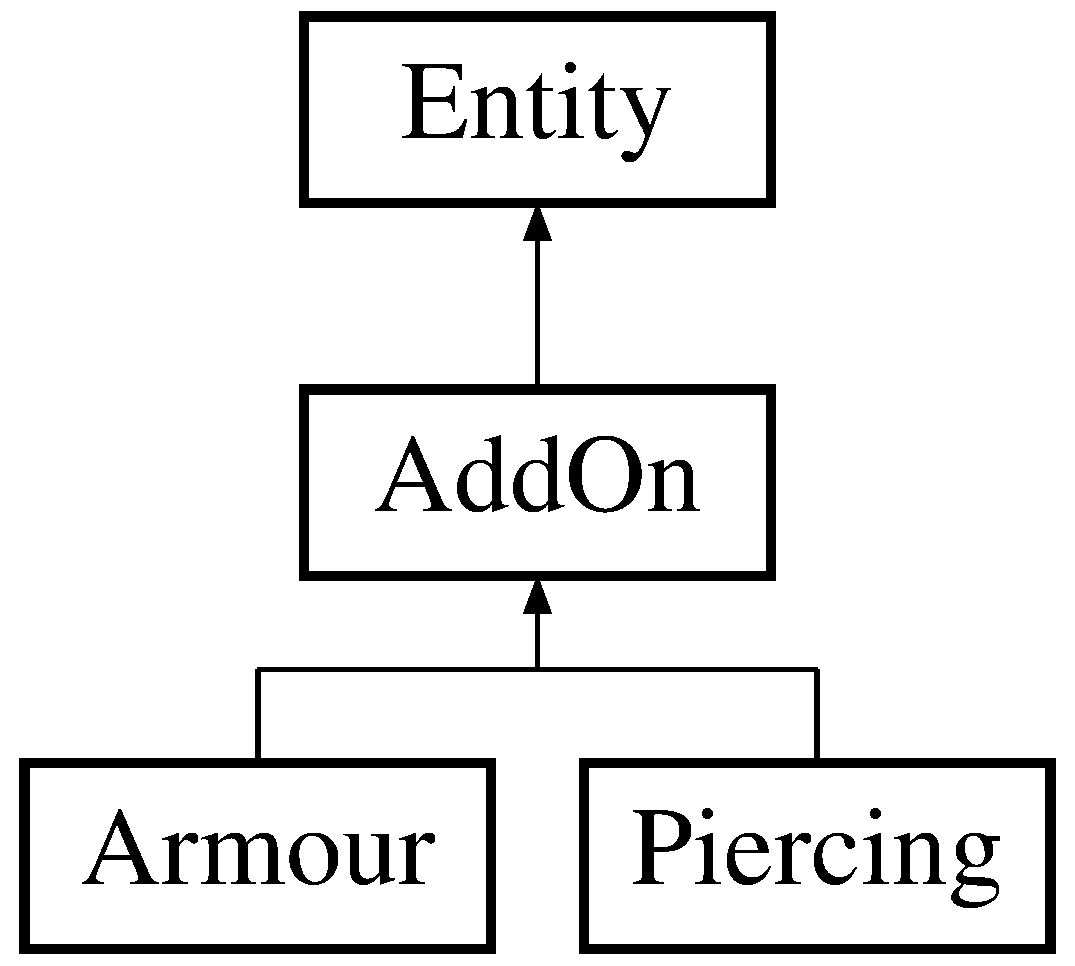
\includegraphics[height=3.000000cm]{classAddOn}
\end{center}
\end{figure}
\doxysubsection*{Public Member Functions}
\begin{DoxyCompactItemize}
\item 
\mbox{\hyperlink{classAddOn_a64f23691b6c7fc49b6584f8f761ce4d9}{Add\+On}} (int value)
\begin{DoxyCompactList}\small\item\em Instantiates an \mbox{\hyperlink{classAddOn}{Add\+On}}. \end{DoxyCompactList}\item 
void \mbox{\hyperlink{classAddOn_a19f4fe81bd1f0491764e52b48a0b3e63}{set\+Value}} (int value)
\begin{DoxyCompactList}\small\item\em Sets the \mbox{\hyperlink{classAddOn}{Add\+On}}\textquotesingle{}s value attribute. \end{DoxyCompactList}\item 
int \mbox{\hyperlink{classAddOn_a776b1f929793e8387cb0b58fc7aba2c2}{get\+Value}} ()
\begin{DoxyCompactList}\small\item\em Returns the \mbox{\hyperlink{classAddOn}{Add\+On}}\textquotesingle{}s value attribute. \end{DoxyCompactList}\item 
void \mbox{\hyperlink{classAddOn_ac9f4263e3558015fdad46adefceed197}{set\+Entity}} (\mbox{\hyperlink{classEntity}{Entity}} $\ast$entity)
\begin{DoxyCompactList}\small\item\em Sets the \mbox{\hyperlink{classAddOn}{Add\+On}}\textquotesingle{}s entity attribute. \end{DoxyCompactList}\item 
\mbox{\hyperlink{classEntity}{Entity}} $\ast$ \mbox{\hyperlink{classAddOn_aaf2f3af4104c7cb69ac67766790ce393}{get\+Entity}} ()
\begin{DoxyCompactList}\small\item\em Returns the \mbox{\hyperlink{classAddOn}{Add\+On}}\textquotesingle{}s entity attribute. \end{DoxyCompactList}\item 
\mbox{\hyperlink{classType}{Type}} $\ast$ \mbox{\hyperlink{classAddOn_a0c194386be045169d3bd923e22c75705}{get\+Type}} ()
\begin{DoxyCompactList}\small\item\em Returns entities type state. \end{DoxyCompactList}\item 
void \mbox{\hyperlink{classAddOn_a3bb07ac367f2fe96e782f84fa48bfc68}{set\+Type}} (\mbox{\hyperlink{classType}{Type}} $\ast$type)
\begin{DoxyCompactList}\small\item\em Sets the entities type state. \end{DoxyCompactList}\item 
\mbox{\hyperlink{classAlliance}{Alliance}} $\ast$ \mbox{\hyperlink{classAddOn_a226cff3c3072cdda884d6d6d8eb74773}{get\+Alliance}} ()
\begin{DoxyCompactList}\small\item\em Returns entities alliance. \end{DoxyCompactList}\item 
void \mbox{\hyperlink{classAddOn_a8ae6d54cdc26e057777f75ff5a45455b}{set\+Alliance}} (\mbox{\hyperlink{classAlliance}{Alliance}} $\ast$alliance)
\begin{DoxyCompactList}\small\item\em Sets the entities alliance. \end{DoxyCompactList}\item 
int \mbox{\hyperlink{classAddOn_a754a8bf01cdd118173ebc0818943dfe7}{get\+Health}} ()
\begin{DoxyCompactList}\small\item\em Returns entities health. \end{DoxyCompactList}\item 
void \mbox{\hyperlink{classAddOn_a24d16b33c873be77c9370ae08a3d617d}{set\+Health}} (int health)
\begin{DoxyCompactList}\small\item\em Sets the entities health. \end{DoxyCompactList}\item 
int \mbox{\hyperlink{classAddOn_a7931cff84029baa9532f6a7c971a5198}{get\+Damage}} ()
\begin{DoxyCompactList}\small\item\em Returns entities damage. \end{DoxyCompactList}\item 
void \mbox{\hyperlink{classAddOn_a37de5bfa51cbf1d65b0bdf612f12065f}{set\+Damage}} (int damage)
\begin{DoxyCompactList}\small\item\em Sets the entities damage. \end{DoxyCompactList}\item 
virtual void \mbox{\hyperlink{classAddOn_ab3aefbc00969fe613ed6d42c4f55c5a2}{take\+Damage}} (int damage)=0
\begin{DoxyCompactList}\small\item\em Reduces health from the \mbox{\hyperlink{classEntity}{Entity}} object. \end{DoxyCompactList}\item 
virtual void \mbox{\hyperlink{classAddOn_aff1f4fa0fb368bbc49838df9c9ddba9c}{deal\+Damage}} (\mbox{\hyperlink{classEntity}{Entity}} $\ast$entity)=0
\begin{DoxyCompactList}\small\item\em Inflicts damage onto another entity. \end{DoxyCompactList}\item 
virtual \mbox{\hyperlink{classAddOn}{Add\+On}} $\ast$ \mbox{\hyperlink{classAddOn_a51874d0b945e57cd2917ef6f25147277}{clone}} ()=0
\begin{DoxyCompactList}\small\item\em Clones the \mbox{\hyperlink{classAddOn}{Add\+On}}\textquotesingle{}s object and returns the the cloned object. \end{DoxyCompactList}\end{DoxyCompactItemize}
\doxysubsection*{Protected Attributes}
\begin{DoxyCompactItemize}
\item 
int \mbox{\hyperlink{classAddOn_a5c051eef3f3e8200d5a48cfc50174f91}{value}}
\item 
\mbox{\hyperlink{classEntity}{Entity}} $\ast$ \mbox{\hyperlink{classAddOn_aaa321002131799f305663626784e364e}{entity}}
\end{DoxyCompactItemize}


\doxysubsection{Detailed Description}
\mbox{\hyperlink{classAddOn}{Add\+On}} class. 

Used to add addtional functionality to \mbox{\hyperlink{classEntity}{Entity}} objects. 

Definition at line \mbox{\hyperlink{AddOn_8h_source_l00010}{10}} of file \mbox{\hyperlink{AddOn_8h_source}{Add\+On.\+h}}.



\doxysubsection{Constructor \& Destructor Documentation}
\mbox{\Hypertarget{classAddOn_a64f23691b6c7fc49b6584f8f761ce4d9}\label{classAddOn_a64f23691b6c7fc49b6584f8f761ce4d9}} 
\index{AddOn@{AddOn}!AddOn@{AddOn}}
\index{AddOn@{AddOn}!AddOn@{AddOn}}
\doxysubsubsection{\texorpdfstring{AddOn()}{AddOn()}}
{\footnotesize\ttfamily Add\+On\+::\+Add\+On (\begin{DoxyParamCaption}\item[{int}]{value }\end{DoxyParamCaption})}



Instantiates an \mbox{\hyperlink{classAddOn}{Add\+On}}. 


\begin{DoxyParams}{Parameters}
{\em value} & must be an int \\
\hline
\end{DoxyParams}


Definition at line \mbox{\hyperlink{AddOn_8cpp_source_l00004}{4}} of file \mbox{\hyperlink{AddOn_8cpp_source}{Add\+On.\+cpp}}.


\begin{DoxyCode}{0}
\DoxyCodeLine{00004                      : \mbox{\hyperlink{classEntity}{Entity}}() \{}
\DoxyCodeLine{00005     this-\/>value = value;}
\DoxyCodeLine{00006     entity = NULL;}
\DoxyCodeLine{00007 \}}

\end{DoxyCode}


\doxysubsection{Member Function Documentation}
\mbox{\Hypertarget{classAddOn_a51874d0b945e57cd2917ef6f25147277}\label{classAddOn_a51874d0b945e57cd2917ef6f25147277}} 
\index{AddOn@{AddOn}!clone@{clone}}
\index{clone@{clone}!AddOn@{AddOn}}
\doxysubsubsection{\texorpdfstring{clone()}{clone()}}
{\footnotesize\ttfamily virtual \mbox{\hyperlink{classAddOn}{Add\+On}} $\ast$ Add\+On\+::clone (\begin{DoxyParamCaption}{ }\end{DoxyParamCaption})\hspace{0.3cm}{\ttfamily [pure virtual]}}



Clones the \mbox{\hyperlink{classAddOn}{Add\+On}}\textquotesingle{}s object and returns the the cloned object. 

Post\+Conditions\+:
\begin{DoxyItemize}
\item The returns the cloned object of \mbox{\hyperlink{classAddOn}{Add\+On}} object
\end{DoxyItemize}

\begin{DoxyReturn}{Returns}
Add\+On$\ast$ the return object 
\end{DoxyReturn}


Implements \mbox{\hyperlink{classEntity_af6107392c2c813bedbc7994618b395db}{Entity}}.



Implemented in \mbox{\hyperlink{classArmour_ab200b02561ecc30c20397913a2bc9511}{Armour}}, and \mbox{\hyperlink{classPiercing_aeb41b04515f5aad4d9f153b0de332849}{Piercing}}.

\mbox{\Hypertarget{classAddOn_aff1f4fa0fb368bbc49838df9c9ddba9c}\label{classAddOn_aff1f4fa0fb368bbc49838df9c9ddba9c}} 
\index{AddOn@{AddOn}!dealDamage@{dealDamage}}
\index{dealDamage@{dealDamage}!AddOn@{AddOn}}
\doxysubsubsection{\texorpdfstring{dealDamage()}{dealDamage()}}
{\footnotesize\ttfamily virtual void Add\+On\+::deal\+Damage (\begin{DoxyParamCaption}\item[{\mbox{\hyperlink{classEntity}{Entity}} $\ast$}]{entity }\end{DoxyParamCaption})\hspace{0.3cm}{\ttfamily [pure virtual]}}



Inflicts damage onto another entity. 

Preconditions\+:
\begin{DoxyItemize}
\item entity must be an Entity$\ast$
\end{DoxyItemize}

Postconditions\+:
\begin{DoxyItemize}
\item Reduces the health of the entity
\end{DoxyItemize}


\begin{DoxyParams}{Parameters}
{\em entity} & must be an Entity$\ast$ \\
\hline
\end{DoxyParams}
\begin{DoxyReturn}{Returns}
void 
\end{DoxyReturn}


Implements \mbox{\hyperlink{classEntity_aff881f545fc88b2c328ff559a99c7fba}{Entity}}.



Implemented in \mbox{\hyperlink{classArmour_acce6c768aaebaa559ac063e9d67c53b5}{Armour}}, and \mbox{\hyperlink{classPiercing_a2dbd4a497f9abbebbbd2ceb2909f6163}{Piercing}}.

\mbox{\Hypertarget{classAddOn_a226cff3c3072cdda884d6d6d8eb74773}\label{classAddOn_a226cff3c3072cdda884d6d6d8eb74773}} 
\index{AddOn@{AddOn}!getAlliance@{getAlliance}}
\index{getAlliance@{getAlliance}!AddOn@{AddOn}}
\doxysubsubsection{\texorpdfstring{getAlliance()}{getAlliance()}}
{\footnotesize\ttfamily \mbox{\hyperlink{classAlliance}{Alliance}} $\ast$ Add\+On\+::get\+Alliance (\begin{DoxyParamCaption}{ }\end{DoxyParamCaption})\hspace{0.3cm}{\ttfamily [virtual]}}



Returns entities alliance. 

Postconditions\+:
\begin{DoxyItemize}
\item Returns the alliance
\end{DoxyItemize}

\begin{DoxyReturn}{Returns}
Type$\ast$ The alliance of the entity object 
\end{DoxyReturn}


Reimplemented from \mbox{\hyperlink{classEntity_aa101047a4bc312b697b65b4c3a39ffc5}{Entity}}.



Definition at line \mbox{\hyperlink{AddOn_8cpp_source_l00037}{37}} of file \mbox{\hyperlink{AddOn_8cpp_source}{Add\+On.\+cpp}}.


\begin{DoxyCode}{0}
\DoxyCodeLine{00037                              \{}
\DoxyCodeLine{00038     \textcolor{keywordflow}{return} entity-\/>\mbox{\hyperlink{classEntity_aa101047a4bc312b697b65b4c3a39ffc5}{getAlliance}}();}
\DoxyCodeLine{00039 \}}

\end{DoxyCode}
\mbox{\Hypertarget{classAddOn_a7931cff84029baa9532f6a7c971a5198}\label{classAddOn_a7931cff84029baa9532f6a7c971a5198}} 
\index{AddOn@{AddOn}!getDamage@{getDamage}}
\index{getDamage@{getDamage}!AddOn@{AddOn}}
\doxysubsubsection{\texorpdfstring{getDamage()}{getDamage()}}
{\footnotesize\ttfamily int Add\+On\+::get\+Damage (\begin{DoxyParamCaption}{ }\end{DoxyParamCaption})\hspace{0.3cm}{\ttfamily [virtual]}}



Returns entities damage. 

Postconditions\+:
\begin{DoxyItemize}
\item Returns the damage
\end{DoxyItemize}

\begin{DoxyReturn}{Returns}
int The damage of the entity object 
\end{DoxyReturn}


Reimplemented from \mbox{\hyperlink{classEntity_ad38d4384aa0adef43443666a33f06508}{Entity}}.



Definition at line \mbox{\hyperlink{AddOn_8cpp_source_l00053}{53}} of file \mbox{\hyperlink{AddOn_8cpp_source}{Add\+On.\+cpp}}.


\begin{DoxyCode}{0}
\DoxyCodeLine{00053                      \{}
\DoxyCodeLine{00054     \textcolor{keywordflow}{return} entity-\/>\mbox{\hyperlink{classEntity_ad38d4384aa0adef43443666a33f06508}{getDamage}}();}
\DoxyCodeLine{00055 \}}

\end{DoxyCode}
\mbox{\Hypertarget{classAddOn_aaf2f3af4104c7cb69ac67766790ce393}\label{classAddOn_aaf2f3af4104c7cb69ac67766790ce393}} 
\index{AddOn@{AddOn}!getEntity@{getEntity}}
\index{getEntity@{getEntity}!AddOn@{AddOn}}
\doxysubsubsection{\texorpdfstring{getEntity()}{getEntity()}}
{\footnotesize\ttfamily \mbox{\hyperlink{classEntity}{Entity}} $\ast$ Add\+On\+::get\+Entity (\begin{DoxyParamCaption}{ }\end{DoxyParamCaption})}



Returns the \mbox{\hyperlink{classAddOn}{Add\+On}}\textquotesingle{}s entity attribute. 

Postconditions\+:
\begin{DoxyItemize}
\item Returns the entity attribute of the \mbox{\hyperlink{classAddOn}{Add\+On}} object
\end{DoxyItemize}

\begin{DoxyReturn}{Returns}
Entity$\ast$ The entity of the \mbox{\hyperlink{classAddOn}{Add\+On}} 
\end{DoxyReturn}


Definition at line \mbox{\hyperlink{AddOn_8cpp_source_l00025}{25}} of file \mbox{\hyperlink{AddOn_8cpp_source}{Add\+On.\+cpp}}.


\begin{DoxyCode}{0}
\DoxyCodeLine{00025                          \{}
\DoxyCodeLine{00026     \textcolor{keywordflow}{return} this-\/>entity;}
\DoxyCodeLine{00027 \}}

\end{DoxyCode}
\mbox{\Hypertarget{classAddOn_a754a8bf01cdd118173ebc0818943dfe7}\label{classAddOn_a754a8bf01cdd118173ebc0818943dfe7}} 
\index{AddOn@{AddOn}!getHealth@{getHealth}}
\index{getHealth@{getHealth}!AddOn@{AddOn}}
\doxysubsubsection{\texorpdfstring{getHealth()}{getHealth()}}
{\footnotesize\ttfamily int Add\+On\+::get\+Health (\begin{DoxyParamCaption}{ }\end{DoxyParamCaption})\hspace{0.3cm}{\ttfamily [virtual]}}



Returns entities health. 

Postconditions\+:
\begin{DoxyItemize}
\item Returns the health
\end{DoxyItemize}

\begin{DoxyReturn}{Returns}
int The health of the entity object 
\end{DoxyReturn}


Reimplemented from \mbox{\hyperlink{classEntity_a2b0140ae8c77c0e3654b070ee3c7fe57}{Entity}}.



Definition at line \mbox{\hyperlink{AddOn_8cpp_source_l00045}{45}} of file \mbox{\hyperlink{AddOn_8cpp_source}{Add\+On.\+cpp}}.


\begin{DoxyCode}{0}
\DoxyCodeLine{00045                      \{}
\DoxyCodeLine{00046     \textcolor{keywordflow}{return} entity-\/>\mbox{\hyperlink{classEntity_a2b0140ae8c77c0e3654b070ee3c7fe57}{getHealth}}();}
\DoxyCodeLine{00047 \}}

\end{DoxyCode}
\mbox{\Hypertarget{classAddOn_a0c194386be045169d3bd923e22c75705}\label{classAddOn_a0c194386be045169d3bd923e22c75705}} 
\index{AddOn@{AddOn}!getType@{getType}}
\index{getType@{getType}!AddOn@{AddOn}}
\doxysubsubsection{\texorpdfstring{getType()}{getType()}}
{\footnotesize\ttfamily \mbox{\hyperlink{classType}{Type}} $\ast$ Add\+On\+::get\+Type (\begin{DoxyParamCaption}{ }\end{DoxyParamCaption})\hspace{0.3cm}{\ttfamily [virtual]}}



Returns entities type state. 

Postconditions\+:
\begin{DoxyItemize}
\item Returns the type
\end{DoxyItemize}

\begin{DoxyReturn}{Returns}
Type$\ast$ The type state of the entity object 
\end{DoxyReturn}


Reimplemented from \mbox{\hyperlink{classEntity_a3a9c9e298bfc47b726a2d9ce44dd7464}{Entity}}.



Definition at line \mbox{\hyperlink{AddOn_8cpp_source_l00029}{29}} of file \mbox{\hyperlink{AddOn_8cpp_source}{Add\+On.\+cpp}}.


\begin{DoxyCode}{0}
\DoxyCodeLine{00029                      \{}
\DoxyCodeLine{00030     \textcolor{keywordflow}{return} entity-\/>\mbox{\hyperlink{classEntity_a3a9c9e298bfc47b726a2d9ce44dd7464}{getType}}();}
\DoxyCodeLine{00031 \}}

\end{DoxyCode}
\mbox{\Hypertarget{classAddOn_a776b1f929793e8387cb0b58fc7aba2c2}\label{classAddOn_a776b1f929793e8387cb0b58fc7aba2c2}} 
\index{AddOn@{AddOn}!getValue@{getValue}}
\index{getValue@{getValue}!AddOn@{AddOn}}
\doxysubsubsection{\texorpdfstring{getValue()}{getValue()}}
{\footnotesize\ttfamily int Add\+On\+::get\+Value (\begin{DoxyParamCaption}{ }\end{DoxyParamCaption})}



Returns the \mbox{\hyperlink{classAddOn}{Add\+On}}\textquotesingle{}s value attribute. 

Postconditions\+:
\begin{DoxyItemize}
\item Returns the value attribute of the \mbox{\hyperlink{classAddOn}{Add\+On}} object
\end{DoxyItemize}

\begin{DoxyReturn}{Returns}
int The values of the \mbox{\hyperlink{classAddOn}{Add\+On}} 
\end{DoxyReturn}


Definition at line \mbox{\hyperlink{AddOn_8cpp_source_l00017}{17}} of file \mbox{\hyperlink{AddOn_8cpp_source}{Add\+On.\+cpp}}.


\begin{DoxyCode}{0}
\DoxyCodeLine{00017                     \{}
\DoxyCodeLine{00018     \textcolor{keywordflow}{return} value;}
\DoxyCodeLine{00019 \}}

\end{DoxyCode}
\mbox{\Hypertarget{classAddOn_a8ae6d54cdc26e057777f75ff5a45455b}\label{classAddOn_a8ae6d54cdc26e057777f75ff5a45455b}} 
\index{AddOn@{AddOn}!setAlliance@{setAlliance}}
\index{setAlliance@{setAlliance}!AddOn@{AddOn}}
\doxysubsubsection{\texorpdfstring{setAlliance()}{setAlliance()}}
{\footnotesize\ttfamily void Add\+On\+::set\+Alliance (\begin{DoxyParamCaption}\item[{\mbox{\hyperlink{classAlliance}{Alliance}} $\ast$}]{alliance }\end{DoxyParamCaption})\hspace{0.3cm}{\ttfamily [virtual]}}



Sets the entities alliance. 

Preconditions\+:
\begin{DoxyItemize}
\item alliance must be an Alliance$\ast$
\end{DoxyItemize}

Postconditions\+:
\begin{DoxyItemize}
\item Sets the alliance of the entity object
\end{DoxyItemize}


\begin{DoxyParams}{Parameters}
{\em alliance} & must be a Alliance$\ast$ \\
\hline
\end{DoxyParams}
\begin{DoxyReturn}{Returns}
void 
\end{DoxyReturn}


Reimplemented from \mbox{\hyperlink{classEntity_af804dcaa600e770cf0e2b4537f6fba23}{Entity}}.



Definition at line \mbox{\hyperlink{AddOn_8cpp_source_l00041}{41}} of file \mbox{\hyperlink{AddOn_8cpp_source}{Add\+On.\+cpp}}.


\begin{DoxyCode}{0}
\DoxyCodeLine{00041                                           \{}
\DoxyCodeLine{00042     entity-\/>\mbox{\hyperlink{classEntity_af804dcaa600e770cf0e2b4537f6fba23}{setAlliance}}(alliance);}
\DoxyCodeLine{00043 \}}

\end{DoxyCode}
\mbox{\Hypertarget{classAddOn_a37de5bfa51cbf1d65b0bdf612f12065f}\label{classAddOn_a37de5bfa51cbf1d65b0bdf612f12065f}} 
\index{AddOn@{AddOn}!setDamage@{setDamage}}
\index{setDamage@{setDamage}!AddOn@{AddOn}}
\doxysubsubsection{\texorpdfstring{setDamage()}{setDamage()}}
{\footnotesize\ttfamily void Add\+On\+::set\+Damage (\begin{DoxyParamCaption}\item[{int}]{damage }\end{DoxyParamCaption})\hspace{0.3cm}{\ttfamily [virtual]}}



Sets the entities damage. 

Preconditions\+:
\begin{DoxyItemize}
\item damage must be an int
\end{DoxyItemize}

Postconditions\+:
\begin{DoxyItemize}
\item Sets the damage of the entity object
\end{DoxyItemize}


\begin{DoxyParams}{Parameters}
{\em damage} & must be an int \\
\hline
\end{DoxyParams}
\begin{DoxyReturn}{Returns}
void 
\end{DoxyReturn}


Reimplemented from \mbox{\hyperlink{classEntity_aae05f62767eb7438c846300704f9579b}{Entity}}.



Definition at line \mbox{\hyperlink{AddOn_8cpp_source_l00057}{57}} of file \mbox{\hyperlink{AddOn_8cpp_source}{Add\+On.\+cpp}}.


\begin{DoxyCode}{0}
\DoxyCodeLine{00057                                 \{}
\DoxyCodeLine{00058     entity-\/>\mbox{\hyperlink{classEntity_aae05f62767eb7438c846300704f9579b}{setDamage}}(damage);}
\DoxyCodeLine{00059 \}}

\end{DoxyCode}
\mbox{\Hypertarget{classAddOn_ac9f4263e3558015fdad46adefceed197}\label{classAddOn_ac9f4263e3558015fdad46adefceed197}} 
\index{AddOn@{AddOn}!setEntity@{setEntity}}
\index{setEntity@{setEntity}!AddOn@{AddOn}}
\doxysubsubsection{\texorpdfstring{setEntity()}{setEntity()}}
{\footnotesize\ttfamily void Add\+On\+::set\+Entity (\begin{DoxyParamCaption}\item[{\mbox{\hyperlink{classEntity}{Entity}} $\ast$}]{entity }\end{DoxyParamCaption})}



Sets the \mbox{\hyperlink{classAddOn}{Add\+On}}\textquotesingle{}s entity attribute. 

Preconditions\+:
\begin{DoxyItemize}
\item entity must be an Entity$\ast$
\end{DoxyItemize}

Postconditions\+:
\begin{DoxyItemize}
\item Sets the entity attribute of the \mbox{\hyperlink{classAddOn}{Add\+On}} object to the passed in entity
\end{DoxyItemize}


\begin{DoxyParams}{Parameters}
{\em entity} & must be an Entity$\ast$ \\
\hline
\end{DoxyParams}
\begin{DoxyReturn}{Returns}
void 
\end{DoxyReturn}


Definition at line \mbox{\hyperlink{AddOn_8cpp_source_l00021}{21}} of file \mbox{\hyperlink{AddOn_8cpp_source}{Add\+On.\+cpp}}.


\begin{DoxyCode}{0}
\DoxyCodeLine{00021                                     \{}
\DoxyCodeLine{00022     this-\/>entity = entity;}
\DoxyCodeLine{00023 \}}

\end{DoxyCode}
\mbox{\Hypertarget{classAddOn_a24d16b33c873be77c9370ae08a3d617d}\label{classAddOn_a24d16b33c873be77c9370ae08a3d617d}} 
\index{AddOn@{AddOn}!setHealth@{setHealth}}
\index{setHealth@{setHealth}!AddOn@{AddOn}}
\doxysubsubsection{\texorpdfstring{setHealth()}{setHealth()}}
{\footnotesize\ttfamily void Add\+On\+::set\+Health (\begin{DoxyParamCaption}\item[{int}]{health }\end{DoxyParamCaption})\hspace{0.3cm}{\ttfamily [virtual]}}



Sets the entities health. 

Preconditions\+:
\begin{DoxyItemize}
\item health must be an int
\end{DoxyItemize}

Postconditions\+:
\begin{DoxyItemize}
\item Sets the health of the entity object
\end{DoxyItemize}


\begin{DoxyParams}{Parameters}
{\em health} & must be an int \\
\hline
\end{DoxyParams}
\begin{DoxyReturn}{Returns}
void 
\end{DoxyReturn}


Reimplemented from \mbox{\hyperlink{classEntity_a7dae281ff92be9bc98672cafe05c77ab}{Entity}}.



Definition at line \mbox{\hyperlink{AddOn_8cpp_source_l00049}{49}} of file \mbox{\hyperlink{AddOn_8cpp_source}{Add\+On.\+cpp}}.


\begin{DoxyCode}{0}
\DoxyCodeLine{00049                                 \{}
\DoxyCodeLine{00050     entity-\/>\mbox{\hyperlink{classEntity_a7dae281ff92be9bc98672cafe05c77ab}{setHealth}}(health);}
\DoxyCodeLine{00051 \}}

\end{DoxyCode}
\mbox{\Hypertarget{classAddOn_a3bb07ac367f2fe96e782f84fa48bfc68}\label{classAddOn_a3bb07ac367f2fe96e782f84fa48bfc68}} 
\index{AddOn@{AddOn}!setType@{setType}}
\index{setType@{setType}!AddOn@{AddOn}}
\doxysubsubsection{\texorpdfstring{setType()}{setType()}}
{\footnotesize\ttfamily void Add\+On\+::set\+Type (\begin{DoxyParamCaption}\item[{\mbox{\hyperlink{classType}{Type}} $\ast$}]{type }\end{DoxyParamCaption})\hspace{0.3cm}{\ttfamily [virtual]}}



Sets the entities type state. 

Preconditions\+:
\begin{DoxyItemize}
\item type must be an Type$\ast$
\end{DoxyItemize}

Postconditions\+:
\begin{DoxyItemize}
\item Sets the type state of the entity object
\end{DoxyItemize}


\begin{DoxyParams}{Parameters}
{\em type} & must be a Type$\ast$ \\
\hline
\end{DoxyParams}
\begin{DoxyReturn}{Returns}
void 
\end{DoxyReturn}


Reimplemented from \mbox{\hyperlink{classEntity_a5d04ce64c9ca214900422865e298e36c}{Entity}}.



Definition at line \mbox{\hyperlink{AddOn_8cpp_source_l00033}{33}} of file \mbox{\hyperlink{AddOn_8cpp_source}{Add\+On.\+cpp}}.


\begin{DoxyCode}{0}
\DoxyCodeLine{00033                               \{}
\DoxyCodeLine{00034     entity-\/>\mbox{\hyperlink{classEntity_a5d04ce64c9ca214900422865e298e36c}{setType}}(type);}
\DoxyCodeLine{00035 \}}

\end{DoxyCode}
\mbox{\Hypertarget{classAddOn_a19f4fe81bd1f0491764e52b48a0b3e63}\label{classAddOn_a19f4fe81bd1f0491764e52b48a0b3e63}} 
\index{AddOn@{AddOn}!setValue@{setValue}}
\index{setValue@{setValue}!AddOn@{AddOn}}
\doxysubsubsection{\texorpdfstring{setValue()}{setValue()}}
{\footnotesize\ttfamily void Add\+On\+::set\+Value (\begin{DoxyParamCaption}\item[{int}]{value }\end{DoxyParamCaption})}



Sets the \mbox{\hyperlink{classAddOn}{Add\+On}}\textquotesingle{}s value attribute. 

Preconditions\+:
\begin{DoxyItemize}
\item value must be an int
\end{DoxyItemize}

Postconditions\+:
\begin{DoxyItemize}
\item Sets the value attribute of the \mbox{\hyperlink{classAddOn}{Add\+On}} object to the passed in value
\end{DoxyItemize}


\begin{DoxyParams}{Parameters}
{\em value} & must be an int \\
\hline
\end{DoxyParams}
\begin{DoxyReturn}{Returns}
void 
\end{DoxyReturn}


Definition at line \mbox{\hyperlink{AddOn_8cpp_source_l00009}{9}} of file \mbox{\hyperlink{AddOn_8cpp_source}{Add\+On.\+cpp}}.


\begin{DoxyCode}{0}
\DoxyCodeLine{00009                               \{}
\DoxyCodeLine{00010 }
\DoxyCodeLine{00011     \textcolor{keywordflow}{if} (value <= 0)}
\DoxyCodeLine{00012         \textcolor{keywordflow}{throw} std::invalid\_argument(\textcolor{stringliteral}{"{}value must be greater than zero"{}});}
\DoxyCodeLine{00013     }
\DoxyCodeLine{00014     this-\/>value = value;}
\DoxyCodeLine{00015 \}}

\end{DoxyCode}
\mbox{\Hypertarget{classAddOn_ab3aefbc00969fe613ed6d42c4f55c5a2}\label{classAddOn_ab3aefbc00969fe613ed6d42c4f55c5a2}} 
\index{AddOn@{AddOn}!takeDamage@{takeDamage}}
\index{takeDamage@{takeDamage}!AddOn@{AddOn}}
\doxysubsubsection{\texorpdfstring{takeDamage()}{takeDamage()}}
{\footnotesize\ttfamily virtual void Add\+On\+::take\+Damage (\begin{DoxyParamCaption}\item[{int}]{damage }\end{DoxyParamCaption})\hspace{0.3cm}{\ttfamily [pure virtual]}}



Reduces health from the \mbox{\hyperlink{classEntity}{Entity}} object. 

Preconditions\+:
\begin{DoxyItemize}
\item damage must be an int
\end{DoxyItemize}

Postconditions\+:
\begin{DoxyItemize}
\item Reduces the health of the \mbox{\hyperlink{classEntity}{Entity}} object
\end{DoxyItemize}


\begin{DoxyParams}{Parameters}
{\em damage} & must be an int \\
\hline
\end{DoxyParams}
\begin{DoxyReturn}{Returns}
void 
\end{DoxyReturn}


Implements \mbox{\hyperlink{classEntity_a9cc5a2246a5580ceed0f081c18211e53}{Entity}}.



Implemented in \mbox{\hyperlink{classArmour_a7a52bd8473173c81a4ba8a6373513581}{Armour}}, and \mbox{\hyperlink{classPiercing_a103634469a43e1662bd5e07e66901667}{Piercing}}.



\doxysubsection{Member Data Documentation}
\mbox{\Hypertarget{classAddOn_aaa321002131799f305663626784e364e}\label{classAddOn_aaa321002131799f305663626784e364e}} 
\index{AddOn@{AddOn}!entity@{entity}}
\index{entity@{entity}!AddOn@{AddOn}}
\doxysubsubsection{\texorpdfstring{entity}{entity}}
{\footnotesize\ttfamily \mbox{\hyperlink{classEntity}{Entity}}$\ast$ Add\+On\+::entity\hspace{0.3cm}{\ttfamily [protected]}}



Definition at line \mbox{\hyperlink{AddOn_8h_source_l00014}{14}} of file \mbox{\hyperlink{AddOn_8h_source}{Add\+On.\+h}}.

\mbox{\Hypertarget{classAddOn_a5c051eef3f3e8200d5a48cfc50174f91}\label{classAddOn_a5c051eef3f3e8200d5a48cfc50174f91}} 
\index{AddOn@{AddOn}!value@{value}}
\index{value@{value}!AddOn@{AddOn}}
\doxysubsubsection{\texorpdfstring{value}{value}}
{\footnotesize\ttfamily int Add\+On\+::value\hspace{0.3cm}{\ttfamily [protected]}}



Definition at line \mbox{\hyperlink{AddOn_8h_source_l00013}{13}} of file \mbox{\hyperlink{AddOn_8h_source}{Add\+On.\+h}}.



The documentation for this class was generated from the following files\+:\begin{DoxyCompactItemize}
\item 
Add\+On.\+h\item 
Add\+On.\+cpp\end{DoxyCompactItemize}

\hypertarget{classAerialType}{}\doxysection{Aerial\+Type Class Reference}
\label{classAerialType}\index{AerialType@{AerialType}}


\mbox{\hyperlink{classAerialType}{Aerial\+Type}} class.  




{\ttfamily \#include $<$Aerial\+Type.\+h$>$}

Inheritance diagram for Aerial\+Type\+:\begin{figure}[H]
\begin{center}
\leavevmode
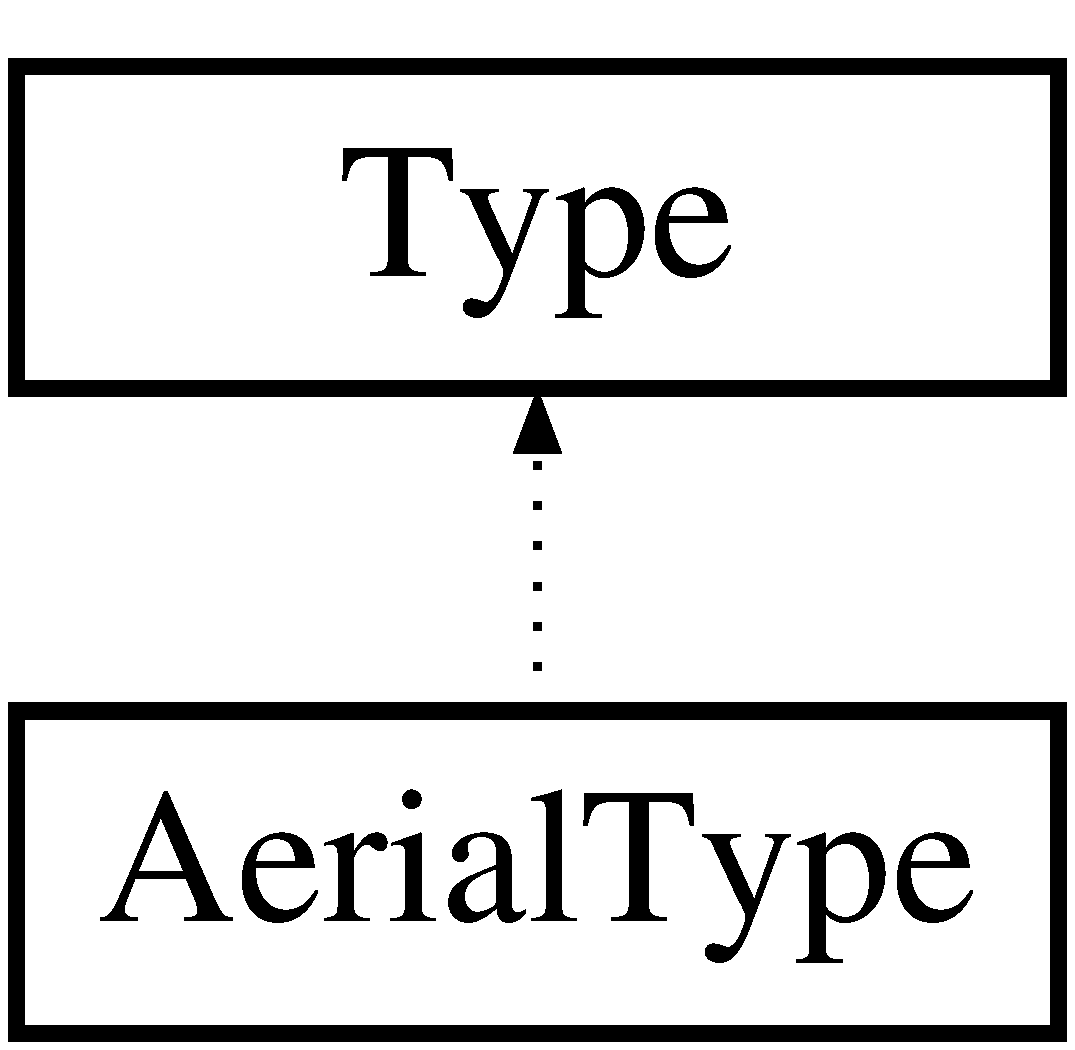
\includegraphics[height=2.000000cm]{classAerialType}
\end{center}
\end{figure}
\doxysubsection*{Public Member Functions}
\begin{DoxyCompactItemize}
\item 
\mbox{\hyperlink{classAerialType_af31f880cd2a2437544e77d38f60d1c99}{Aerial\+Type}} ()
\begin{DoxyCompactList}\small\item\em Instantiates the ariel type. \end{DoxyCompactList}\item 
<<<<<<< HEAD
string \hyperlink{classAerialType_a66dd43f2688de9a5eab9c6de0396e9cc}{get\+Type\+Desc} ()
\begin{DoxyCompactList}\small\item\em Returns ariel type description. \end{DoxyCompactList}\item 
\hyperlink{classType}{Type} $\ast$ \hyperlink{classAerialType_a8e7184b0b9e184142144df65f3da7fb1}{clone} ()
\begin{DoxyCompactList}\small\item\em returns the the cloned object of \hyperlink{classType}{Type} \end{DoxyCompactList}\end{DoxyCompactItemize}
=======
string \mbox{\hyperlink{classAerialType_a66dd43f2688de9a5eab9c6de0396e9cc}{get\+Type\+Desc}} ()
\begin{DoxyCompactList}\small\item\em Returns ariel type description. \end{DoxyCompactList}\item 
\mbox{\hyperlink{classType}{Type}} $\ast$ \mbox{\hyperlink{classAerialType_a8e7184b0b9e184142144df65f3da7fb1}{clone}} ()
\end{DoxyCompactItemize}
>>>>>>> 7be49738cebc0ced3357f2ce74f6fda2ea0b3d5e


\doxysubsection{Detailed Description}
\mbox{\hyperlink{classAerialType}{Aerial\+Type}} class. 

<<<<<<< HEAD
Used to define Entity objects as ariel type. 
=======
Used to define \mbox{\hyperlink{classEntity}{Entity}} objects as ariel type. 
>>>>>>> 7be49738cebc0ced3357f2ce74f6fda2ea0b3d5e

Definition at line \mbox{\hyperlink{AerialType_8h_source_l00011}{11}} of file \mbox{\hyperlink{AerialType_8h_source}{Aerial\+Type.\+h}}.



<<<<<<< HEAD
\subsection{Member Function Documentation}
\mbox{\Hypertarget{classAerialType_a8e7184b0b9e184142144df65f3da7fb1}\label{classAerialType_a8e7184b0b9e184142144df65f3da7fb1}} 
\index{Aerial\+Type@{Aerial\+Type}!clone@{clone}}
\index{clone@{clone}!Aerial\+Type@{Aerial\+Type}}
\subsubsection{\texorpdfstring{clone()}{clone()}}
{\footnotesize\ttfamily \hyperlink{classType}{Type} $\ast$ Aerial\+Type\+::clone (\begin{DoxyParamCaption}{ }\end{DoxyParamCaption})\hspace{0.3cm}{\ttfamily [virtual]}}



returns the the cloned object of \hyperlink{classType}{Type} 

Post\+Conditions\+:
\begin{DoxyItemize}
\item returns Type$\ast$ type
\end{DoxyItemize}

\begin{DoxyReturn}{Returns}
Type$\ast$ The cloned \hyperlink{classType}{Type} object 
\end{DoxyReturn}


Implements \hyperlink{classType_a7b79d264e2cbac9c091cdb41ffb112c9}{Type}.



Definition at line 9 of file Aerial\+Type.\+cpp.


\begin{DoxyCode}
9                         \{
10     \textcolor{keywordflow}{return} \textcolor{keyword}{new} \hyperlink{classAerialType_af31f880cd2a2437544e77d38f60d1c99}{AerialType}();
11 \}
=======
\doxysubsection{Constructor \& Destructor Documentation}
\mbox{\Hypertarget{classAerialType_af31f880cd2a2437544e77d38f60d1c99}\label{classAerialType_af31f880cd2a2437544e77d38f60d1c99}} 
\index{AerialType@{AerialType}!AerialType@{AerialType}}
\index{AerialType@{AerialType}!AerialType@{AerialType}}
\doxysubsubsection{\texorpdfstring{AerialType()}{AerialType()}}
{\footnotesize\ttfamily Aerial\+Type\+::\+Aerial\+Type (\begin{DoxyParamCaption}{ }\end{DoxyParamCaption})}



Instantiates the ariel type. 



Definition at line \mbox{\hyperlink{AerialType_8cpp_source_l00003}{3}} of file \mbox{\hyperlink{AerialType_8cpp_source}{Aerial\+Type.\+cpp}}.


\begin{DoxyCode}{0}
\DoxyCodeLine{00003 \{\}}

\end{DoxyCode}


\doxysubsection{Member Function Documentation}
\mbox{\Hypertarget{classAerialType_a8e7184b0b9e184142144df65f3da7fb1}\label{classAerialType_a8e7184b0b9e184142144df65f3da7fb1}} 
\index{AerialType@{AerialType}!clone@{clone}}
\index{clone@{clone}!AerialType@{AerialType}}
\doxysubsubsection{\texorpdfstring{clone()}{clone()}}
{\footnotesize\ttfamily \mbox{\hyperlink{classType}{Type}} $\ast$ Aerial\+Type\+::clone (\begin{DoxyParamCaption}{ }\end{DoxyParamCaption})\hspace{0.3cm}{\ttfamily [virtual]}}



Implements \mbox{\hyperlink{classType}{Type}}.



Definition at line \mbox{\hyperlink{AerialType_8cpp_source_l00009}{9}} of file \mbox{\hyperlink{AerialType_8cpp_source}{Aerial\+Type.\+cpp}}.


\begin{DoxyCode}{0}
\DoxyCodeLine{00009                         \{}
\DoxyCodeLine{00010     \textcolor{keywordflow}{return} \textcolor{keyword}{new} \mbox{\hyperlink{classAerialType_af31f880cd2a2437544e77d38f60d1c99}{AerialType}}();}
\DoxyCodeLine{00011 \}}

>>>>>>> 7be49738cebc0ced3357f2ce74f6fda2ea0b3d5e
\end{DoxyCode}
\mbox{\Hypertarget{classAerialType_a66dd43f2688de9a5eab9c6de0396e9cc}\label{classAerialType_a66dd43f2688de9a5eab9c6de0396e9cc}} 
\index{AerialType@{AerialType}!getTypeDesc@{getTypeDesc}}
\index{getTypeDesc@{getTypeDesc}!AerialType@{AerialType}}
\doxysubsubsection{\texorpdfstring{getTypeDesc()}{getTypeDesc()}}
{\footnotesize\ttfamily string Aerial\+Type\+::get\+Type\+Desc (\begin{DoxyParamCaption}{ }\end{DoxyParamCaption})\hspace{0.3cm}{\ttfamily [virtual]}}



Returns ariel type description. 

Postconditions\+:
\begin{DoxyItemize}
\item Returns the ariel type
\end{DoxyItemize}

\begin{DoxyReturn}{Returns}
string The ariel type string 
\end{DoxyReturn}


<<<<<<< HEAD
Implements \hyperlink{classType_a5c453300dc060252c30534110bd2f78c}{Type}.
=======
Implements \mbox{\hyperlink{classType}{Type}}.
>>>>>>> 7be49738cebc0ced3357f2ce74f6fda2ea0b3d5e



Definition at line \mbox{\hyperlink{AerialType_8cpp_source_l00005}{5}} of file \mbox{\hyperlink{AerialType_8cpp_source}{Aerial\+Type.\+cpp}}.


\begin{DoxyCode}{0}
\DoxyCodeLine{00005                                \{}
\DoxyCodeLine{00006     \textcolor{keywordflow}{return} \textcolor{stringliteral}{"{}Aerial"{}};}
\DoxyCodeLine{00007 \}}

\end{DoxyCode}


The documentation for this class was generated from the following files\+:\begin{DoxyCompactItemize}
\item 
Aerial\+Type.\+h\item 
Aerial\+Type.\+cpp\end{DoxyCompactItemize}

\hypertarget{classAggressive}{}\section{Aggressive Class Reference}
\label{classAggressive}\index{Aggressive@{Aggressive}}
Inheritance diagram for Aggressive\+:\begin{figure}[H]
\begin{center}
\leavevmode
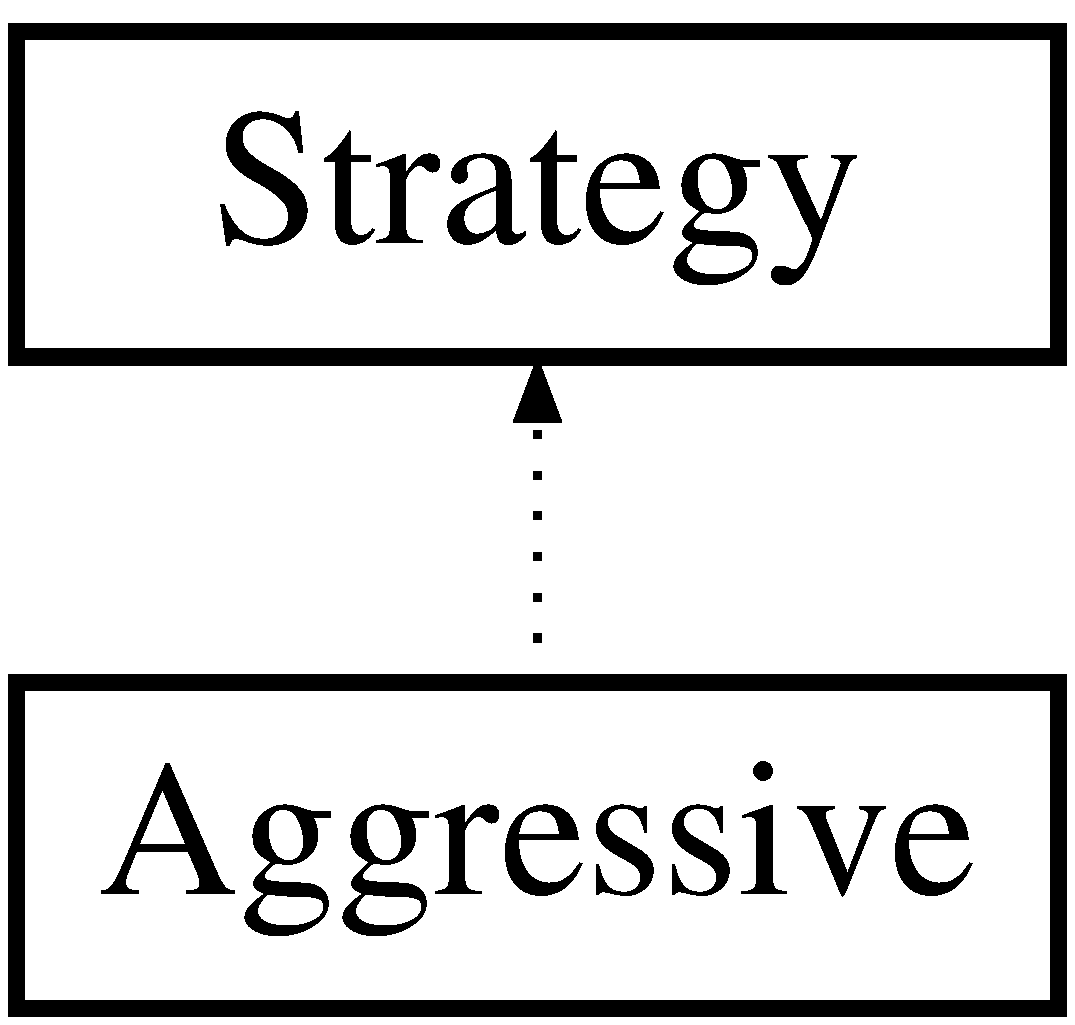
\includegraphics[height=2.000000cm]{classAggressive}
\end{center}
\end{figure}
\subsection*{Public Member Functions}
\begin{DoxyCompactItemize}
\item 
\mbox{\Hypertarget{classAggressive_a0b46e6b9a78e6fc8634e0f2a331987a2}\label{classAggressive_a0b46e6b9a78e6fc8634e0f2a331987a2}} 
\hyperlink{classAggressive_a0b46e6b9a78e6fc8634e0f2a331987a2}{Aggressive} ()
\begin{DoxyCompactList}\small\item\em Construct a new \hyperlink{classAggressive}{Aggressive} object. \end{DoxyCompactList}\item 
\hyperlink{classAggressive_a41f26c922a9794bdf223407201ab4bdd}{$\sim$\+Aggressive} () void \hyperlink{classStrategy_ada170bd47bc6f11ac02d7df2b366387b}{perform\+Strat}(\hyperlink{classKeyPoint}{Key\+Point} $\ast$key\+Point)
\begin{DoxyCompactList}\small\item\em Destroy the \hyperlink{classAggressive}{Aggressive} object. \end{DoxyCompactList}\end{DoxyCompactItemize}
\subsection*{Additional Inherited Members}


\subsection{Detailed Description}


Definition at line 6 of file Aggressive.\+h.



\subsection{Constructor \& Destructor Documentation}
\mbox{\Hypertarget{classAggressive_a41f26c922a9794bdf223407201ab4bdd}\label{classAggressive_a41f26c922a9794bdf223407201ab4bdd}} 
\index{Aggressive@{Aggressive}!````~Aggressive@{$\sim$\+Aggressive}}
\index{````~Aggressive@{$\sim$\+Aggressive}!Aggressive@{Aggressive}}
\subsubsection{\texorpdfstring{$\sim$\+Aggressive()}{~Aggressive()}}
{\footnotesize\ttfamily Aggressive\+::$\sim$\+Aggressive (\begin{DoxyParamCaption}{ }\end{DoxyParamCaption})}



Destroy the \hyperlink{classAggressive}{Aggressive} object. 

\begin{DoxyAuthor}{Author}
Antwi-\/\+Antwi This function will perform an Aggresive strategy 
\end{DoxyAuthor}

\begin{DoxyParams}{Parameters}
{\em key\+Point} & an \hyperlink{classAggressive}{Aggressive} strategy will then be performed at this specific keypoint \\
\hline
\end{DoxyParams}
\begin{DoxyReturn}{Returns}
void The function will return a void 
\end{DoxyReturn}


The documentation for this class was generated from the following files\+:\begin{DoxyCompactItemize}
\item 
Aggressive.\+h\item 
Aggressive.\+cpp\end{DoxyCompactItemize}

\hypertarget{classAlliance}{}\doxysection{Alliance Class Reference}
\label{classAlliance}\index{Alliance@{Alliance}}
\doxysubsection*{Public Member Functions}
\begin{DoxyCompactItemize}
\item 
\mbox{\hyperlink{classAlliance_a262a2819e969b465eb9548e419bad521}{Alliance}} ()
\begin{DoxyCompactList}\small\item\em Instantiates the \mbox{\hyperlink{classAlliance}{Alliance}}. \end{DoxyCompactList}\item 
\mbox{\hyperlink{classAlliance_acde91b73cf63cf19ed13448a8644d139}{Alliance}} (\mbox{\hyperlink{classAlliance}{Alliance}} \&alliance)
\begin{DoxyCompactList}\small\item\em Instantiates a copy of an \mbox{\hyperlink{classAlliance}{Alliance}}. \end{DoxyCompactList}\item 
\mbox{\hyperlink{classAlliance_a6a5357e96f284da2f00d72d14605b6fe}{$\sim$\+Alliance}} ()
\begin{DoxyCompactList}\small\item\em Destructor for the \mbox{\hyperlink{classAlliance}{Alliance}} object. \end{DoxyCompactList}\item 
void \mbox{\hyperlink{classAlliance_ae900967c4bc7a6ee970fbefade816457}{set\+Negotiator}} (\mbox{\hyperlink{classNegotiator}{Negotiator}} $\ast$new\+Negotiator)
\begin{DoxyCompactList}\small\item\em Sets the entity negotiator. \end{DoxyCompactList}\item 
void \mbox{\hyperlink{classAlliance_a5aad3039bd784cb26755fce97c92708a}{add\+Country}} (\mbox{\hyperlink{classCountry}{Country}} $\ast$nation)
\begin{DoxyCompactList}\small\item\em Adds a country into the members vector which holds countries. \end{DoxyCompactList}\item 
vector$<$ \mbox{\hyperlink{classEntity}{Entity}} $\ast$ $>$ \mbox{\hyperlink{classAlliance_a8c93c88d5624a3445814b86496ad68d7}{get\+Reserve\+Entities}} (int number)
\begin{DoxyCompactList}\small\item\em Return a given number of reserve entites vector. \end{DoxyCompactList}\item 
void \mbox{\hyperlink{classAlliance_a37c4045fb37caf729d1f8f266f5f1bf0}{add\+Reserve\+Entity}} (\mbox{\hyperlink{classEntity}{Entity}} $\ast$entity)
\begin{DoxyCompactList}\small\item\em Adds a entity to the reserve entities. \end{DoxyCompactList}\item 
int \mbox{\hyperlink{classAlliance_aa7536e9920dba6e114d77dd18ab0326a}{num\+Remaining\+Entities}} ()
\item 
bool \mbox{\hyperlink{classAlliance_aaa6e77e8bef285079525b65150c3ad85}{consider\+Peace}} ()
\begin{DoxyCompactList}\small\item\em Considers to stop war with the allaince passed into the function header. \end{DoxyCompactList}\item 
void \mbox{\hyperlink{classAlliance_a0558b1f3532044e9b5648c0bd1c151bf}{add\+Factory}} (\mbox{\hyperlink{classFactory}{Factory}} $\ast$factory)
\begin{DoxyCompactList}\small\item\em Adds a factory into the production vector which holds factories. \end{DoxyCompactList}\item 
void \mbox{\hyperlink{classAlliance_a0b0d133ea177694c86d7cc9dd6b05a40}{run\+Factories}} ()
\item 
void \mbox{\hyperlink{classAlliance_ad3b8272ccec63d3a32b7e241434948e9}{surrender}} ()
\begin{DoxyCompactList}\small\item\em Makes the current alliance give up of the war by surrendering. \end{DoxyCompactList}\item 
int \mbox{\hyperlink{classAlliance_a7f23330454f02b0056eb92bd2072359d}{get\+ID}} ()
\begin{DoxyCompactList}\small\item\em Returns \mbox{\hyperlink{classAlliance}{Alliance}}\textquotesingle{}s a\+ID. \end{DoxyCompactList}\item 
bool \mbox{\hyperlink{classAlliance_ad13d2c031669cebc82021e4c2efc2c12}{offer\+Peace}} ()
\begin{DoxyCompactList}\small\item\em Offers peace to stop war with the alliance fighting against using send\+Peace. \end{DoxyCompactList}\item 
\mbox{\hyperlink{classAlliance}{Alliance}} $\ast$ \mbox{\hyperlink{classAlliance_adc67a41223565105889493f9cfd350d0}{clone}} ()
\begin{DoxyCompactList}\small\item\em Instantiates and returns a clone of the current \mbox{\hyperlink{classAlliance}{Alliance}}. \end{DoxyCompactList}\item 
void \mbox{\hyperlink{classAlliance_a21492fd899af1441c9d8ddf11a558e7d}{set\+Active\+Status}} (bool active)
\begin{DoxyCompactList}\small\item\em Sets variable active to the passed in parameter. \end{DoxyCompactList}\item 
int \mbox{\hyperlink{classAlliance_a832ce46bb4b7062240a0586788e3ff59}{get\+Active}} ()
\end{DoxyCompactItemize}


\doxysubsection{Detailed Description}


Definition at line \mbox{\hyperlink{Alliance_8h_source_l00013}{13}} of file \mbox{\hyperlink{Alliance_8h_source}{Alliance.\+h}}.



\doxysubsection{Constructor \& Destructor Documentation}
\mbox{\Hypertarget{classAlliance_a262a2819e969b465eb9548e419bad521}\label{classAlliance_a262a2819e969b465eb9548e419bad521}} 
\index{Alliance@{Alliance}!Alliance@{Alliance}}
\index{Alliance@{Alliance}!Alliance@{Alliance}}
\doxysubsubsection{\texorpdfstring{Alliance()}{Alliance()}\hspace{0.1cm}{\footnotesize\ttfamily [1/2]}}
{\footnotesize\ttfamily Alliance\+::\+Alliance (\begin{DoxyParamCaption}{ }\end{DoxyParamCaption})}



Instantiates the \mbox{\hyperlink{classAlliance}{Alliance}}. 



Definition at line \mbox{\hyperlink{Alliance_8cpp_source_l00012}{12}} of file \mbox{\hyperlink{Alliance_8cpp_source}{Alliance.\+cpp}}.


\begin{DoxyCode}{0}
\DoxyCodeLine{00012                    \{}
\DoxyCodeLine{00013     this-\/>active = 1;}
\DoxyCodeLine{00014     this-\/>aID = totalNum++;}
\DoxyCodeLine{00015     this-\/>negotiator = NULL;}
\DoxyCodeLine{00016     srand(time(0));}
\DoxyCodeLine{00017 \}}

\end{DoxyCode}
\mbox{\Hypertarget{classAlliance_acde91b73cf63cf19ed13448a8644d139}\label{classAlliance_acde91b73cf63cf19ed13448a8644d139}} 
\index{Alliance@{Alliance}!Alliance@{Alliance}}
\index{Alliance@{Alliance}!Alliance@{Alliance}}
\doxysubsubsection{\texorpdfstring{Alliance()}{Alliance()}\hspace{0.1cm}{\footnotesize\ttfamily [2/2]}}
{\footnotesize\ttfamily Alliance\+::\+Alliance (\begin{DoxyParamCaption}\item[{\mbox{\hyperlink{classAlliance}{Alliance}} \&}]{alliance }\end{DoxyParamCaption})}



Instantiates a copy of an \mbox{\hyperlink{classAlliance}{Alliance}}. 


\begin{DoxyParams}{Parameters}
{\em alliance} & must be an alliance instance \\
\hline
\end{DoxyParams}


Definition at line \mbox{\hyperlink{Alliance_8cpp_source_l00019}{19}} of file \mbox{\hyperlink{Alliance_8cpp_source}{Alliance.\+cpp}}.


\begin{DoxyCode}{0}
\DoxyCodeLine{00019                                      \{}
\DoxyCodeLine{00020     this-\/>active = alliance.active;}
\DoxyCodeLine{00021     this-\/>aID = alliance.aID;}
\DoxyCodeLine{00022 }
\DoxyCodeLine{00023     \textcolor{keywordflow}{for} (\textcolor{keywordtype}{int} i = 0; i < alliance.members.size(); i++)}
\DoxyCodeLine{00024         this-\/>\mbox{\hyperlink{classAlliance_a5aad3039bd784cb26755fce97c92708a}{addCountry}}(alliance.members[i]-\/>clone());}
\DoxyCodeLine{00025 }
\DoxyCodeLine{00026     \textcolor{keywordflow}{for} (\textcolor{keywordtype}{int} i = 0; i < alliance.production.size(); i++)}
\DoxyCodeLine{00027         this-\/>\mbox{\hyperlink{classAlliance_a0558b1f3532044e9b5648c0bd1c151bf}{addFactory}}(alliance.production[i]-\/>clone());}
\DoxyCodeLine{00028 }
\DoxyCodeLine{00029     \textcolor{keywordflow}{for} (\textcolor{keywordtype}{int} i = 0; i < alliance.reserveEntities.size(); i++)}
\DoxyCodeLine{00030         this-\/>\mbox{\hyperlink{classAlliance_a37c4045fb37caf729d1f8f266f5f1bf0}{addReserveEntity}}(alliance.reserveEntities[i]-\/>clone());}
\DoxyCodeLine{00031 }
\DoxyCodeLine{00032     this-\/>negotiator = NULL;}
\DoxyCodeLine{00033 \}}

\end{DoxyCode}
\mbox{\Hypertarget{classAlliance_a6a5357e96f284da2f00d72d14605b6fe}\label{classAlliance_a6a5357e96f284da2f00d72d14605b6fe}} 
\index{Alliance@{Alliance}!````~Alliance@{$\sim$Alliance}}
\index{````~Alliance@{$\sim$Alliance}!Alliance@{Alliance}}
\doxysubsubsection{\texorpdfstring{$\sim$Alliance()}{~Alliance()}}
{\footnotesize\ttfamily Alliance\+::$\sim$\+Alliance (\begin{DoxyParamCaption}{ }\end{DoxyParamCaption})}



Destructor for the \mbox{\hyperlink{classAlliance}{Alliance}} object. 



Definition at line \mbox{\hyperlink{Alliance_8cpp_source_l00035}{35}} of file \mbox{\hyperlink{Alliance_8cpp_source}{Alliance.\+cpp}}.


\begin{DoxyCode}{0}
\DoxyCodeLine{00035                     \{}
\DoxyCodeLine{00036 }
\DoxyCodeLine{00037     \textcolor{keywordflow}{for} (\textcolor{keywordtype}{int} i = 0; i < members.size(); i++)}
\DoxyCodeLine{00038         \textcolor{comment}{//delete members[i];}}
\DoxyCodeLine{00039 }
\DoxyCodeLine{00040     \textcolor{keywordflow}{if} (this-\/>negotiator != NULL) \{}
\DoxyCodeLine{00041         this-\/>negotiator-\/>\mbox{\hyperlink{classNegotiator_ac6ec48dbce55bf196c299342695054ef}{removeAlliance}}(\textcolor{keyword}{this});}
\DoxyCodeLine{00042 }
\DoxyCodeLine{00043         \textcolor{keywordflow}{if} (this-\/>negotiator-\/>\mbox{\hyperlink{classNegotiator_a20af02012820a0296ac14f75e0b87282}{getNumAlliances}}() == 1)}
\DoxyCodeLine{00044             \textcolor{keyword}{delete} this-\/>negotiator;}
\DoxyCodeLine{00045     \}}
\DoxyCodeLine{00046 \}}

\end{DoxyCode}


\doxysubsection{Member Function Documentation}
\mbox{\Hypertarget{classAlliance_a5aad3039bd784cb26755fce97c92708a}\label{classAlliance_a5aad3039bd784cb26755fce97c92708a}} 
\index{Alliance@{Alliance}!addCountry@{addCountry}}
\index{addCountry@{addCountry}!Alliance@{Alliance}}
\doxysubsubsection{\texorpdfstring{addCountry()}{addCountry()}}
{\footnotesize\ttfamily void Alliance\+::add\+Country (\begin{DoxyParamCaption}\item[{\mbox{\hyperlink{classCountry}{Country}} $\ast$}]{nation }\end{DoxyParamCaption})}



Adds a country into the members vector which holds countries. 

Preconditions\+:
\begin{DoxyItemize}
\item nation must be an Country$\ast$
\end{DoxyItemize}

Postconditions\+:
\begin{DoxyItemize}
\item \mbox{\hyperlink{classCountry}{Country}} is added to the members vector
\end{DoxyItemize}


\begin{DoxyParams}{Parameters}
{\em nation} & must be an Country$\ast$ \\
\hline
\end{DoxyParams}
\begin{DoxyReturn}{Returns}
void 
\end{DoxyReturn}


Definition at line \mbox{\hyperlink{Alliance_8cpp_source_l00052}{52}} of file \mbox{\hyperlink{Alliance_8cpp_source}{Alliance.\+cpp}}.


\begin{DoxyCode}{0}
\DoxyCodeLine{00052                                          \{}
\DoxyCodeLine{00053     members.push\_back(nation);}
\DoxyCodeLine{00054 \}}

\end{DoxyCode}
\mbox{\Hypertarget{classAlliance_a0558b1f3532044e9b5648c0bd1c151bf}\label{classAlliance_a0558b1f3532044e9b5648c0bd1c151bf}} 
\index{Alliance@{Alliance}!addFactory@{addFactory}}
\index{addFactory@{addFactory}!Alliance@{Alliance}}
\doxysubsubsection{\texorpdfstring{addFactory()}{addFactory()}}
{\footnotesize\ttfamily void Alliance\+::add\+Factory (\begin{DoxyParamCaption}\item[{\mbox{\hyperlink{classFactory}{Factory}} $\ast$}]{factory }\end{DoxyParamCaption})}



Adds a factory into the production vector which holds factories. 

Preconditions\+:
\begin{DoxyItemize}
\item f must be an Factory$\ast$
\end{DoxyItemize}

Postconditions\+:
\begin{DoxyItemize}
\item \mbox{\hyperlink{classFactory}{Factory}} is added to the production vector
\end{DoxyItemize}


\begin{DoxyParams}{Parameters}
{\em factory} & must be a Factory$\ast$ \\
\hline
\end{DoxyParams}
\begin{DoxyReturn}{Returns}
void 
\end{DoxyReturn}


Definition at line \mbox{\hyperlink{Alliance_8cpp_source_l00078}{78}} of file \mbox{\hyperlink{Alliance_8cpp_source}{Alliance.\+cpp}}.


\begin{DoxyCode}{0}
\DoxyCodeLine{00078                                           \{}
\DoxyCodeLine{00079     production.push\_back(factory);}
\DoxyCodeLine{00080 \}}

\end{DoxyCode}
\mbox{\Hypertarget{classAlliance_a37c4045fb37caf729d1f8f266f5f1bf0}\label{classAlliance_a37c4045fb37caf729d1f8f266f5f1bf0}} 
\index{Alliance@{Alliance}!addReserveEntity@{addReserveEntity}}
\index{addReserveEntity@{addReserveEntity}!Alliance@{Alliance}}
\doxysubsubsection{\texorpdfstring{addReserveEntity()}{addReserveEntity()}}
{\footnotesize\ttfamily void Alliance\+::add\+Reserve\+Entity (\begin{DoxyParamCaption}\item[{\mbox{\hyperlink{classEntity}{Entity}} $\ast$}]{entity }\end{DoxyParamCaption})}



Adds a entity to the reserve entities. 

Preconditions\+:
\begin{DoxyItemize}
\item nation must be an Entity$\ast$
\end{DoxyItemize}

Postconditions\+:
\begin{DoxyItemize}
\item \mbox{\hyperlink{classEntity}{Entity}} is added to the reserve\+Entities vector
\end{DoxyItemize}


\begin{DoxyParams}{Parameters}
{\em entity} & must be an Entity$\ast$ \\
\hline
\end{DoxyParams}
\begin{DoxyReturn}{Returns}
void 
\end{DoxyReturn}


Definition at line \mbox{\hyperlink{Alliance_8cpp_source_l00066}{66}} of file \mbox{\hyperlink{Alliance_8cpp_source}{Alliance.\+cpp}}.


\begin{DoxyCode}{0}
\DoxyCodeLine{00066                                               \{}
\DoxyCodeLine{00067     reserveEntities.push\_back(entity);}
\DoxyCodeLine{00068 \}}

\end{DoxyCode}
\mbox{\Hypertarget{classAlliance_adc67a41223565105889493f9cfd350d0}\label{classAlliance_adc67a41223565105889493f9cfd350d0}} 
\index{Alliance@{Alliance}!clone@{clone}}
\index{clone@{clone}!Alliance@{Alliance}}
\doxysubsubsection{\texorpdfstring{clone()}{clone()}}
{\footnotesize\ttfamily \mbox{\hyperlink{classAlliance}{Alliance}} $\ast$ Alliance\+::clone (\begin{DoxyParamCaption}{ }\end{DoxyParamCaption})}



Instantiates and returns a clone of the current \mbox{\hyperlink{classAlliance}{Alliance}}. 

Postconditions\+:
\begin{DoxyItemize}
\item Returns the clone of the current \mbox{\hyperlink{classAlliance}{Alliance}}
\end{DoxyItemize}

\begin{DoxyReturn}{Returns}
Alliance$\ast$ The alliance clone 
\end{DoxyReturn}


Definition at line \mbox{\hyperlink{Alliance_8cpp_source_l00114}{114}} of file \mbox{\hyperlink{Alliance_8cpp_source}{Alliance.\+cpp}}.


\begin{DoxyCode}{0}
\DoxyCodeLine{00114                           \{}
\DoxyCodeLine{00115     \textcolor{keywordflow}{return} \textcolor{keyword}{new} \mbox{\hyperlink{classAlliance_a262a2819e969b465eb9548e419bad521}{Alliance}}(*\textcolor{keyword}{this});}
\DoxyCodeLine{00116 \}}

\end{DoxyCode}
\mbox{\Hypertarget{classAlliance_aaa6e77e8bef285079525b65150c3ad85}\label{classAlliance_aaa6e77e8bef285079525b65150c3ad85}} 
\index{Alliance@{Alliance}!considerPeace@{considerPeace}}
\index{considerPeace@{considerPeace}!Alliance@{Alliance}}
\doxysubsubsection{\texorpdfstring{considerPeace()}{considerPeace()}}
{\footnotesize\ttfamily bool Alliance\+::consider\+Peace (\begin{DoxyParamCaption}{ }\end{DoxyParamCaption})}



Considers to stop war with the allaince passed into the function header. 

Preconditions\+:
\begin{DoxyItemize}
\item id must be an integer
\end{DoxyItemize}

Postconditions\+:
\begin{DoxyItemize}
\item Result of consideration returned in the form of a bool
\end{DoxyItemize}

\begin{DoxyReturn}{Returns}
bool 
\end{DoxyReturn}


Definition at line \mbox{\hyperlink{Alliance_8cpp_source_l00074}{74}} of file \mbox{\hyperlink{Alliance_8cpp_source}{Alliance.\+cpp}}.


\begin{DoxyCode}{0}
\DoxyCodeLine{00074                              \{}
\DoxyCodeLine{00075     \textcolor{keywordflow}{return} (rand() \% 2 == 0);}
\DoxyCodeLine{00076 \}}

\end{DoxyCode}
\mbox{\Hypertarget{classAlliance_a832ce46bb4b7062240a0586788e3ff59}\label{classAlliance_a832ce46bb4b7062240a0586788e3ff59}} 
\index{Alliance@{Alliance}!getActive@{getActive}}
\index{getActive@{getActive}!Alliance@{Alliance}}
\doxysubsubsection{\texorpdfstring{getActive()}{getActive()}}
{\footnotesize\ttfamily int Alliance\+::get\+Active (\begin{DoxyParamCaption}{ }\end{DoxyParamCaption})}



Definition at line \mbox{\hyperlink{Alliance_8cpp_source_l00110}{110}} of file \mbox{\hyperlink{Alliance_8cpp_source}{Alliance.\+cpp}}.


\begin{DoxyCode}{0}
\DoxyCodeLine{00110                         \{}
\DoxyCodeLine{00111     \textcolor{keywordflow}{return} active;}
\DoxyCodeLine{00112 \}}

\end{DoxyCode}
\mbox{\Hypertarget{classAlliance_a7f23330454f02b0056eb92bd2072359d}\label{classAlliance_a7f23330454f02b0056eb92bd2072359d}} 
\index{Alliance@{Alliance}!getID@{getID}}
\index{getID@{getID}!Alliance@{Alliance}}
\doxysubsubsection{\texorpdfstring{getID()}{getID()}}
{\footnotesize\ttfamily int Alliance\+::get\+ID (\begin{DoxyParamCaption}{ }\end{DoxyParamCaption})}



Returns \mbox{\hyperlink{classAlliance}{Alliance}}\textquotesingle{}s a\+ID. 

Postconditions\+:
\begin{DoxyItemize}
\item Returns the a\+ID
\end{DoxyItemize}

\begin{DoxyReturn}{Returns}
int The ID of the \mbox{\hyperlink{classAlliance}{Alliance}} object 
\end{DoxyReturn}


Definition at line \mbox{\hyperlink{Alliance_8cpp_source_l00095}{95}} of file \mbox{\hyperlink{Alliance_8cpp_source}{Alliance.\+cpp}}.


\begin{DoxyCode}{0}
\DoxyCodeLine{00095                     \{}
\DoxyCodeLine{00096     \textcolor{keywordflow}{return} this-\/>aID;}
\DoxyCodeLine{00097 \}}

\end{DoxyCode}
\mbox{\Hypertarget{classAlliance_a8c93c88d5624a3445814b86496ad68d7}\label{classAlliance_a8c93c88d5624a3445814b86496ad68d7}} 
\index{Alliance@{Alliance}!getReserveEntities@{getReserveEntities}}
\index{getReserveEntities@{getReserveEntities}!Alliance@{Alliance}}
\doxysubsubsection{\texorpdfstring{getReserveEntities()}{getReserveEntities()}}
{\footnotesize\ttfamily vector$<$ \mbox{\hyperlink{classEntity}{Entity}} $\ast$ $>$ Alliance\+::get\+Reserve\+Entities (\begin{DoxyParamCaption}\item[{int}]{number }\end{DoxyParamCaption})}



Return a given number of reserve entites vector. 

Precondition\+:
\begin{DoxyItemize}
\item number must be an int
\end{DoxyItemize}

Postconditions\+:
\begin{DoxyItemize}
\item Return a given number of reserve entities
\item If not enough reseverves return amount available
\end{DoxyItemize}


\begin{DoxyParams}{Parameters}
{\em number} & must be an int \\
\hline
\end{DoxyParams}
\begin{DoxyReturn}{Returns}
vector$<$\+Entity$\ast$$>$$\ast$ 
\end{DoxyReturn}


Definition at line \mbox{\hyperlink{Alliance_8cpp_source_l00056}{56}} of file \mbox{\hyperlink{Alliance_8cpp_source}{Alliance.\+cpp}}.


\begin{DoxyCode}{0}
\DoxyCodeLine{00056                                                        \{}
\DoxyCodeLine{00057     vector<Entity*> out;}
\DoxyCodeLine{00058     \textcolor{keywordflow}{for} (\textcolor{keywordtype}{int} i = 0; i < number \&\& i < reserveEntities.size(); i++) \{}
\DoxyCodeLine{00059         out.push\_back(reserveEntities[i]);}
\DoxyCodeLine{00060         reserveEntities.erase(reserveEntities.begin() + i);}
\DoxyCodeLine{00061     \}}
\DoxyCodeLine{00062 }
\DoxyCodeLine{00063     \textcolor{keywordflow}{return} out;}
\DoxyCodeLine{00064 \}   }

\end{DoxyCode}
\mbox{\Hypertarget{classAlliance_aa7536e9920dba6e114d77dd18ab0326a}\label{classAlliance_aa7536e9920dba6e114d77dd18ab0326a}} 
\index{Alliance@{Alliance}!numRemainingEntities@{numRemainingEntities}}
\index{numRemainingEntities@{numRemainingEntities}!Alliance@{Alliance}}
\doxysubsubsection{\texorpdfstring{numRemainingEntities()}{numRemainingEntities()}}
{\footnotesize\ttfamily int Alliance\+::num\+Remaining\+Entities (\begin{DoxyParamCaption}{ }\end{DoxyParamCaption})}



Definition at line \mbox{\hyperlink{Alliance_8cpp_source_l00070}{70}} of file \mbox{\hyperlink{Alliance_8cpp_source}{Alliance.\+cpp}}.


\begin{DoxyCode}{0}
\DoxyCodeLine{00070                                    \{}
\DoxyCodeLine{00071     \textcolor{keywordflow}{return} reserveEntities.size();}
\DoxyCodeLine{00072 \}}

\end{DoxyCode}
\mbox{\Hypertarget{classAlliance_ad13d2c031669cebc82021e4c2efc2c12}\label{classAlliance_ad13d2c031669cebc82021e4c2efc2c12}} 
\index{Alliance@{Alliance}!offerPeace@{offerPeace}}
\index{offerPeace@{offerPeace}!Alliance@{Alliance}}
\doxysubsubsection{\texorpdfstring{offerPeace()}{offerPeace()}}
{\footnotesize\ttfamily bool Alliance\+::offer\+Peace (\begin{DoxyParamCaption}{ }\end{DoxyParamCaption})}



Offers peace to stop war with the alliance fighting against using send\+Peace. 

Postconditions\+:
\begin{DoxyItemize}
\item Result of consideration returned from the enemy alliance which considered peace
\end{DoxyItemize}

\begin{DoxyReturn}{Returns}
bool 
\end{DoxyReturn}


Definition at line \mbox{\hyperlink{Alliance_8cpp_source_l00099}{99}} of file \mbox{\hyperlink{Alliance_8cpp_source}{Alliance.\+cpp}}.


\begin{DoxyCode}{0}
\DoxyCodeLine{00099                           \{}
\DoxyCodeLine{00100 }
\DoxyCodeLine{00101     \textcolor{keywordflow}{if} (this-\/>negotiator-\/>\mbox{\hyperlink{classNegotiator_aa95e7f447a76c6d5ef84b92731ccb00d}{sendPeace}}(\textcolor{keyword}{this})) \textcolor{comment}{//Send the peace deal to all the alliances fighting against}}
\DoxyCodeLine{00102     \{}
\DoxyCodeLine{00103         this-\/>active = 3; \textcolor{comment}{//Number 3 means that Alliance chose to peacefully pull out of war}}
\DoxyCodeLine{00104         \textcolor{keywordflow}{return} \textcolor{keyword}{true};}
\DoxyCodeLine{00105     \}}
\DoxyCodeLine{00106     }
\DoxyCodeLine{00107     \textcolor{keywordflow}{return} \textcolor{keyword}{false}; }
\DoxyCodeLine{00108 \}}

\end{DoxyCode}
\mbox{\Hypertarget{classAlliance_a0b0d133ea177694c86d7cc9dd6b05a40}\label{classAlliance_a0b0d133ea177694c86d7cc9dd6b05a40}} 
\index{Alliance@{Alliance}!runFactories@{runFactories}}
\index{runFactories@{runFactories}!Alliance@{Alliance}}
\doxysubsubsection{\texorpdfstring{runFactories()}{runFactories()}}
{\footnotesize\ttfamily void Alliance\+::run\+Factories (\begin{DoxyParamCaption}{ }\end{DoxyParamCaption})}



Definition at line \mbox{\hyperlink{Alliance_8cpp_source_l00082}{82}} of file \mbox{\hyperlink{Alliance_8cpp_source}{Alliance.\+cpp}}.


\begin{DoxyCode}{0}
\DoxyCodeLine{00082                             \{}
\DoxyCodeLine{00083     \textcolor{keywordflow}{for} (\textcolor{keywordtype}{int} i = 0; i < production.size(); i++) \{}
\DoxyCodeLine{00084         RoundStats::numEntitiesCreated++;}
\DoxyCodeLine{00085         reserveEntities.push\_back(production[i]-\/>createEntity(\textcolor{keyword}{this}));}
\DoxyCodeLine{00086     \}}
\DoxyCodeLine{00087 \}}

\end{DoxyCode}
\mbox{\Hypertarget{classAlliance_a21492fd899af1441c9d8ddf11a558e7d}\label{classAlliance_a21492fd899af1441c9d8ddf11a558e7d}} 
\index{Alliance@{Alliance}!setActiveStatus@{setActiveStatus}}
\index{setActiveStatus@{setActiveStatus}!Alliance@{Alliance}}
\doxysubsubsection{\texorpdfstring{setActiveStatus()}{setActiveStatus()}}
{\footnotesize\ttfamily void Alliance\+::set\+Active\+Status (\begin{DoxyParamCaption}\item[{bool}]{active }\end{DoxyParamCaption})}



Sets variable active to the passed in parameter. 

Pre\+Condtions\+:
\begin{DoxyItemize}
\item active must be an a bool
\end{DoxyItemize}

Post\+Conditions\+:
\begin{DoxyItemize}
\item The varriable active is set to the passed in the parameter
\end{DoxyItemize}


\begin{DoxyParams}{Parameters}
{\em ID} & a bool parameter \\
\hline
\end{DoxyParams}
\mbox{\Hypertarget{classAlliance_ae900967c4bc7a6ee970fbefade816457}\label{classAlliance_ae900967c4bc7a6ee970fbefade816457}} 
\index{Alliance@{Alliance}!setNegotiator@{setNegotiator}}
\index{setNegotiator@{setNegotiator}!Alliance@{Alliance}}
\doxysubsubsection{\texorpdfstring{setNegotiator()}{setNegotiator()}}
{\footnotesize\ttfamily void Alliance\+::set\+Negotiator (\begin{DoxyParamCaption}\item[{\mbox{\hyperlink{classNegotiator}{Negotiator}} $\ast$}]{new\+Negotiator }\end{DoxyParamCaption})}



Sets the entity negotiator. 

Preconditions\+:
\begin{DoxyItemize}
\item n must be an Negotiator$\ast$
\end{DoxyItemize}

Postconditions\+:
\begin{DoxyItemize}
\item Sets the negotiator of the \mbox{\hyperlink{classAlliance}{Alliance}} object
\end{DoxyItemize}


\begin{DoxyParams}{Parameters}
{\em n} & must be a Negotiator$\ast$ \\
\hline
\end{DoxyParams}
\begin{DoxyReturn}{Returns}
void 
\end{DoxyReturn}


Definition at line \mbox{\hyperlink{Alliance_8cpp_source_l00048}{48}} of file \mbox{\hyperlink{Alliance_8cpp_source}{Alliance.\+cpp}}.


\begin{DoxyCode}{0}
\DoxyCodeLine{00048                                                    \{}
\DoxyCodeLine{00049     this-\/>negotiator = negotiator;}
\DoxyCodeLine{00050 \}}

\end{DoxyCode}
\mbox{\Hypertarget{classAlliance_ad3b8272ccec63d3a32b7e241434948e9}\label{classAlliance_ad3b8272ccec63d3a32b7e241434948e9}} 
\index{Alliance@{Alliance}!surrender@{surrender}}
\index{surrender@{surrender}!Alliance@{Alliance}}
\doxysubsubsection{\texorpdfstring{surrender()}{surrender()}}
{\footnotesize\ttfamily void Alliance\+::surrender (\begin{DoxyParamCaption}{ }\end{DoxyParamCaption})}



Makes the current alliance give up of the war by surrendering. 

Postconditions\+:
\begin{DoxyItemize}
\item Sets the active variable to false
\item Removes this alliance from the \mbox{\hyperlink{classNegotiator}{Negotiator}} vector
\end{DoxyItemize}

\begin{DoxyReturn}{Returns}
void 
\end{DoxyReturn}


Definition at line \mbox{\hyperlink{Alliance_8cpp_source_l00089}{89}} of file \mbox{\hyperlink{Alliance_8cpp_source}{Alliance.\+cpp}}.


\begin{DoxyCode}{0}
\DoxyCodeLine{00089                          \{}
\DoxyCodeLine{00090     this-\/>active = 2; \textcolor{comment}{//Number 2 means that Alliance has surrendered}}
\DoxyCodeLine{00091 }
\DoxyCodeLine{00092     this-\/>negotiator-\/>\mbox{\hyperlink{classNegotiator_ac6ec48dbce55bf196c299342695054ef}{removeAlliance}}(\textcolor{keyword}{this});}
\DoxyCodeLine{00093 \}}

\end{DoxyCode}


The documentation for this class was generated from the following files\+:\begin{DoxyCompactItemize}
\item 
Alliance.\+h\item 
Alliance.\+cpp\end{DoxyCompactItemize}

\hypertarget{classAquaticType}{}\doxysection{Aquatic\+Type Class Reference}
\label{classAquaticType}\index{AquaticType@{AquaticType}}
Inheritance diagram for Aquatic\+Type\+:\begin{figure}[H]
\begin{center}
\leavevmode
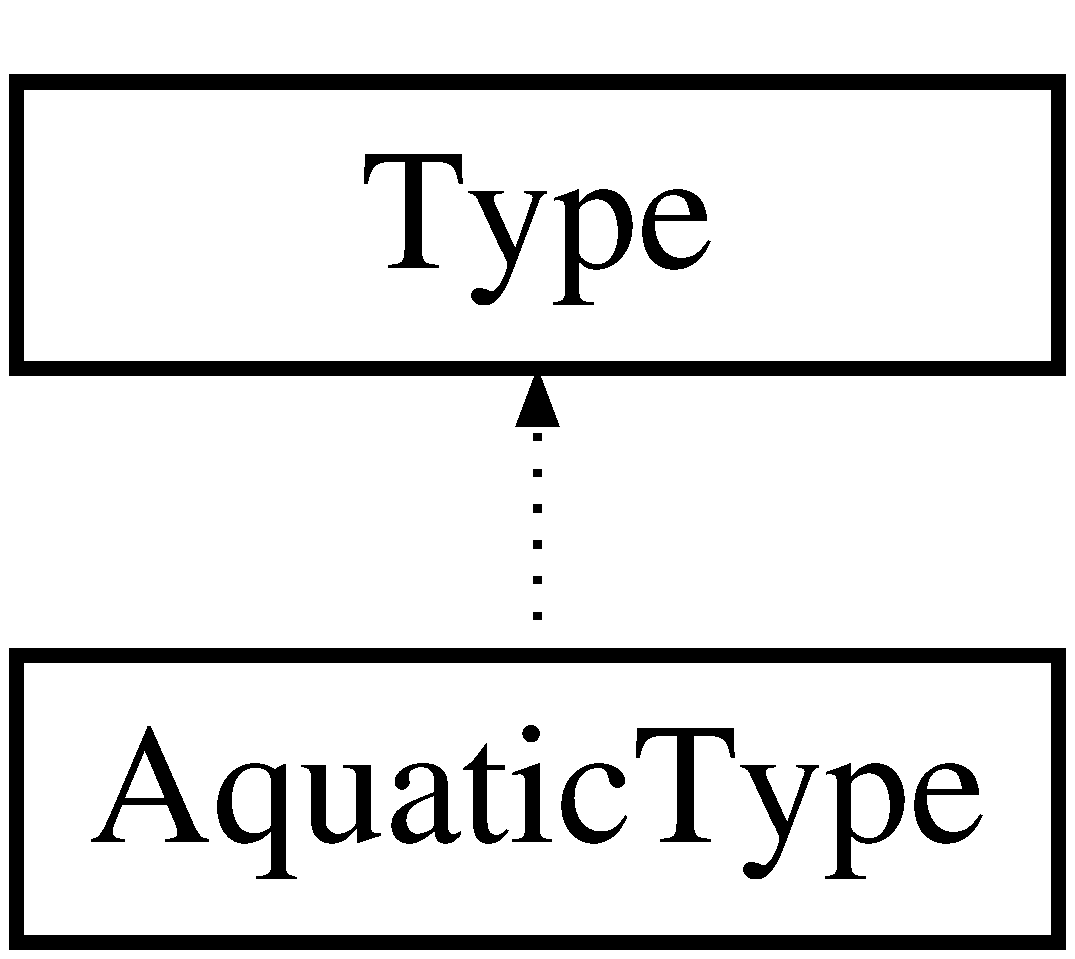
\includegraphics[height=2.000000cm]{classAquaticType}
\end{center}
\end{figure}
\doxysubsection*{Public Member Functions}
\begin{DoxyCompactItemize}
\item 
\mbox{\Hypertarget{classAquaticType_a2e9287ecb48a58ca5d8fd560da4d9d57}\label{classAquaticType_a2e9287ecb48a58ca5d8fd560da4d9d57}} 
\mbox{\hyperlink{classAquaticType_a2e9287ecb48a58ca5d8fd560da4d9d57}{Aquatic\+Type}} ()
\begin{DoxyCompactList}\small\item\em Instantiates the aquatic type. \end{DoxyCompactList}\item 
string \mbox{\hyperlink{classAquaticType_abb1b9ebdb96a352e0287f7a7cb803eab}{get\+Type\+Desc}} ()
\begin{DoxyCompactList}\small\item\em Returns aquatic type description. \end{DoxyCompactList}\end{DoxyCompactItemize}


\doxysubsection{Detailed Description}


Definition at line 4 of file Aquatic\+Type.\+h.



\doxysubsection{Member Function Documentation}
\mbox{\Hypertarget{classAquaticType_abb1b9ebdb96a352e0287f7a7cb803eab}\label{classAquaticType_abb1b9ebdb96a352e0287f7a7cb803eab}} 
\index{AquaticType@{AquaticType}!getTypeDesc@{getTypeDesc}}
\index{getTypeDesc@{getTypeDesc}!AquaticType@{AquaticType}}
\doxysubsubsection{\texorpdfstring{getTypeDesc()}{getTypeDesc()}}
{\footnotesize\ttfamily string Aquatic\+Type\+::get\+Type\+Desc (\begin{DoxyParamCaption}{ }\end{DoxyParamCaption})\hspace{0.3cm}{\ttfamily [virtual]}}



Returns aquatic type description. 

Postconditions\+:
\begin{DoxyItemize}
\item Returns the aquatic type
\end{DoxyItemize}

\begin{DoxyReturn}{Returns}
string The aquatic type string 
\end{DoxyReturn}


Implements \mbox{\hyperlink{classType}{Type}}.



Definition at line 10 of file Aquatic\+Type.\+cpp.


\begin{DoxyCode}{0}
\DoxyCodeLine{10                                 \{}
\DoxyCodeLine{11     \textcolor{comment}{// TODO -\/ implement AquaticType::getTypeDesc}}
\DoxyCodeLine{12     \textcolor{keywordflow}{throw} \textcolor{stringliteral}{"Not yet implemented"};}
\DoxyCodeLine{13 \}}

\end{DoxyCode}


The documentation for this class was generated from the following files\+:\begin{DoxyCompactItemize}
\item 
Aquatic\+Type.\+h\item 
Aquatic\+Type.\+cpp\end{DoxyCompactItemize}

\hypertarget{classArea}{}\doxysection{Area Class Reference}
\label{classArea}\index{Area@{Area}}
Inheritance diagram for Area\+:\begin{figure}[H]
\begin{center}
\leavevmode
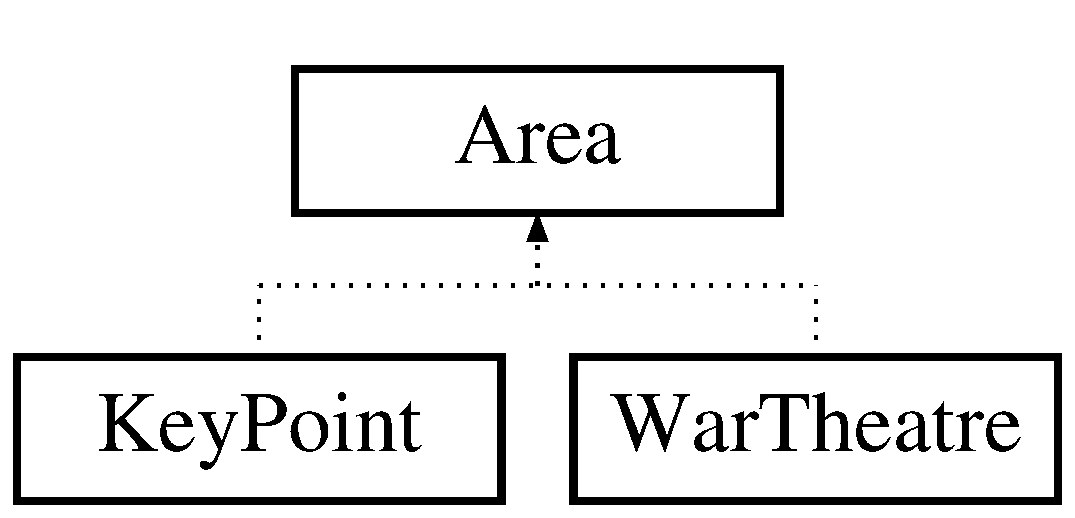
\includegraphics[height=2.000000cm]{classArea}
\end{center}
\end{figure}
\doxysubsection*{Public Member Functions}
\begin{DoxyCompactItemize}
\item 
<<<<<<< HEAD
\mbox{\Hypertarget{classArea_a765c2ee1798421e3079ab77f97abf367}\label{classArea_a765c2ee1798421e3079ab77f97abf367}} 
\hyperlink{classArea_a765c2ee1798421e3079ab77f97abf367}{Area} (std\+::string area\+Name)
\begin{DoxyCompactList}\small\item\em Instantiates the area. \end{DoxyCompactList}\item 
\mbox{\Hypertarget{classArea_ace0975982b61a16746c564a0d43a4cc8}\label{classArea_ace0975982b61a16746c564a0d43a4cc8}} 
virtual \hyperlink{classArea_ace0975982b61a16746c564a0d43a4cc8}{$\sim$\+Area} ()
=======
\mbox{\hyperlink{classArea_a765c2ee1798421e3079ab77f97abf367}{Area}} (std\+::string area\+Name)
\begin{DoxyCompactList}\small\item\em Instantiates the area. \end{DoxyCompactList}\item 
virtual \mbox{\hyperlink{classArea_ace0975982b61a16746c564a0d43a4cc8}{$\sim$\+Area}} ()
>>>>>>> 7be49738cebc0ced3357f2ce74f6fda2ea0b3d5e
\begin{DoxyCompactList}\small\item\em Destroys the area object. \end{DoxyCompactList}\item 
virtual bool \mbox{\hyperlink{classArea_a5572fd57878be1d0d1f243de4be742db}{is\+Key\+Point}} ()=0
\item 
<<<<<<< HEAD
\mbox{\Hypertarget{classArea_a21450849c93621152b13bafcf6e248d5}\label{classArea_a21450849c93621152b13bafcf6e248d5}} 
virtual void {\bfseries simulate\+Battle} (Alliance $\ast$alliance)=0
\item 
std\+::string \hyperlink{classArea_ad67916df281b6b172c4423627b65062a}{get\+Area\+Name} () const
\begin{DoxyCompactList}\small\item\em Get the \hyperlink{classArea}{Area} \hyperlink{classType}{Type} object. \end{DoxyCompactList}\item 
virtual \hyperlink{classArea}{Area} $\ast$ \hyperlink{classArea_a383d61c76b8fac66ef903036d776a3a4}{clone} ()=0
\begin{DoxyCompactList}\small\item\em Instantiates and returns a clone of the current war theatre. \end{DoxyCompactList}\item 
\mbox{\Hypertarget{classArea_ae3e229ab4fb2e5b19fc8cfedf078bc95}\label{classArea_ae3e229ab4fb2e5b19fc8cfedf078bc95}} 
virtual void {\bfseries add\+General} (\hyperlink{classGeneral}{General} $\ast$general)=0
=======
virtual void \mbox{\hyperlink{classArea_a21450849c93621152b13bafcf6e248d5}{simulate\+Battle}} (\mbox{\hyperlink{classAlliance}{Alliance}} $\ast$alliance)=0
\item 
std\+::string \mbox{\hyperlink{classArea_ad67916df281b6b172c4423627b65062a}{get\+Area\+Name}} () const
\begin{DoxyCompactList}\small\item\em Get the \mbox{\hyperlink{classArea}{Area}} \mbox{\hyperlink{classType}{Type}} object. \end{DoxyCompactList}\item 
virtual \mbox{\hyperlink{classArea}{Area}} $\ast$ \mbox{\hyperlink{classArea_a8f95bd4832e9534e645403975435b11d}{clone}} ()=0
<<<<<<< HEAD
\item 
virtual void \mbox{\hyperlink{classArea_ae3e229ab4fb2e5b19fc8cfedf078bc95}{add\+General}} (\mbox{\hyperlink{classGeneral}{General}} $\ast$general)=0
=======
>>>>>>> 7be49738cebc0ced3357f2ce74f6fda2ea0b3d5e
>>>>>>> 033252bd2b51b3f8b7b40b7810d1efb339e193d9
\end{DoxyCompactItemize}


\doxysubsection{Detailed Description}


<<<<<<< HEAD
Definition at line \mbox{\hyperlink{Area_8h_source_l00008}{8}} of file \mbox{\hyperlink{Area_8h_source}{Area.\+h}}.
=======
<<<<<<< HEAD
Definition at line 8 of file Area.\+h.
=======
Definition at line \mbox{\hyperlink{Area_8h_source_l00006}{6}} of file \mbox{\hyperlink{Area_8h_source}{Area.\+h}}.
>>>>>>> 033252bd2b51b3f8b7b40b7810d1efb339e193d9



\doxysubsection{Constructor \& Destructor Documentation}
\mbox{\Hypertarget{classArea_a765c2ee1798421e3079ab77f97abf367}\label{classArea_a765c2ee1798421e3079ab77f97abf367}} 
\index{Area@{Area}!Area@{Area}}
\index{Area@{Area}!Area@{Area}}
\doxysubsubsection{\texorpdfstring{Area()}{Area()}}
{\footnotesize\ttfamily Area\+::\+Area (\begin{DoxyParamCaption}\item[{std\+::string}]{area\+Name }\end{DoxyParamCaption})}



Instantiates the area. 



Definition at line \mbox{\hyperlink{Area_8cpp_source_l00005}{5}} of file \mbox{\hyperlink{Area_8cpp_source}{Area.\+cpp}}.


\begin{DoxyCode}{0}
\DoxyCodeLine{00005                           \{}
\DoxyCodeLine{00006     this-\/>areaName = areaName;}
\DoxyCodeLine{00007 \}}

\end{DoxyCode}
\mbox{\Hypertarget{classArea_ace0975982b61a16746c564a0d43a4cc8}\label{classArea_ace0975982b61a16746c564a0d43a4cc8}} 
\index{Area@{Area}!````~Area@{$\sim$Area}}
\index{````~Area@{$\sim$Area}!Area@{Area}}
\doxysubsubsection{\texorpdfstring{$\sim$Area()}{~Area()}}
{\footnotesize\ttfamily Area\+::$\sim$\+Area (\begin{DoxyParamCaption}{ }\end{DoxyParamCaption})\hspace{0.3cm}{\ttfamily [virtual]}}



Destroys the area object. 



Definition at line \mbox{\hyperlink{Area_8cpp_source_l00009}{9}} of file \mbox{\hyperlink{Area_8cpp_source}{Area.\+cpp}}.


\begin{DoxyCode}{0}
\DoxyCodeLine{00009 \{\}}

\end{DoxyCode}


\doxysubsection{Member Function Documentation}
\mbox{\Hypertarget{classArea_ae3e229ab4fb2e5b19fc8cfedf078bc95}\label{classArea_ae3e229ab4fb2e5b19fc8cfedf078bc95}} 
\index{Area@{Area}!addGeneral@{addGeneral}}
\index{addGeneral@{addGeneral}!Area@{Area}}
\doxysubsubsection{\texorpdfstring{addGeneral()}{addGeneral()}}
{\footnotesize\ttfamily virtual void Area\+::add\+General (\begin{DoxyParamCaption}\item[{\mbox{\hyperlink{classGeneral}{General}} $\ast$}]{general }\end{DoxyParamCaption})\hspace{0.3cm}{\ttfamily [pure virtual]}}



Implemented in \mbox{\hyperlink{classWarTheatre_a1a8640cb110c90f2f2619344fc16a15e}{War\+Theatre}}.

\mbox{\Hypertarget{classArea_a8f95bd4832e9534e645403975435b11d}\label{classArea_a8f95bd4832e9534e645403975435b11d}} 
\index{Area@{Area}!clone@{clone}}
\index{clone@{clone}!Area@{Area}}
\doxysubsubsection{\texorpdfstring{clone()}{clone()}}
{\footnotesize\ttfamily virtual \mbox{\hyperlink{classArea}{Area}} $\ast$ Area\+::clone (\begin{DoxyParamCaption}{ }\end{DoxyParamCaption})\hspace{0.3cm}{\ttfamily [pure virtual]}}



Implemented in \mbox{\hyperlink{classKeyPoint_adc4679ca31d34b0ae3fedded47e27938}{Key\+Point}}, and \mbox{\hyperlink{classWarTheatre_afc32ceef9af26ba4e858c91bf769aef9}{War\+Theatre}}.

\mbox{\Hypertarget{classArea_ad67916df281b6b172c4423627b65062a}\label{classArea_ad67916df281b6b172c4423627b65062a}} 
\index{Area@{Area}!getAreaName@{getAreaName}}
\index{getAreaName@{getAreaName}!Area@{Area}}
\doxysubsubsection{\texorpdfstring{getAreaName()}{getAreaName()}}
{\footnotesize\ttfamily std\+::string Area\+::get\+Area\+Name (\begin{DoxyParamCaption}{ }\end{DoxyParamCaption}) const}



Get the \mbox{\hyperlink{classArea}{Area}} \mbox{\hyperlink{classType}{Type}} object. 

\begin{DoxyReturn}{Returns}
std\+::string reaturns the type 
\end{DoxyReturn}


Definition at line \mbox{\hyperlink{Area_8cpp_source_l00011}{11}} of file \mbox{\hyperlink{Area_8cpp_source}{Area.\+cpp}}.


\begin{DoxyCode}{0}
\DoxyCodeLine{00011                                   \{}
\DoxyCodeLine{00012     \textcolor{keywordflow}{return} areaName;}
\DoxyCodeLine{00013 \}}

\end{DoxyCode}
\mbox{\Hypertarget{classArea_a5572fd57878be1d0d1f243de4be742db}\label{classArea_a5572fd57878be1d0d1f243de4be742db}} 
\index{Area@{Area}!isKeyPoint@{isKeyPoint}}
\index{isKeyPoint@{isKeyPoint}!Area@{Area}}
\doxysubsubsection{\texorpdfstring{isKeyPoint()}{isKeyPoint()}}
{\footnotesize\ttfamily virtual bool Area\+::is\+Key\+Point (\begin{DoxyParamCaption}{ }\end{DoxyParamCaption})\hspace{0.3cm}{\ttfamily [pure virtual]}}



Implemented in \mbox{\hyperlink{classKeyPoint_a1beb436d8efa973f3dc290a722727961}{Key\+Point}}, and \mbox{\hyperlink{classWarTheatre_a01845ca2cc01367101b2884f2902bf88}{War\+Theatre}}.

\mbox{\Hypertarget{classArea_a21450849c93621152b13bafcf6e248d5}\label{classArea_a21450849c93621152b13bafcf6e248d5}} 
\index{Area@{Area}!simulateBattle@{simulateBattle}}
\index{simulateBattle@{simulateBattle}!Area@{Area}}
\doxysubsubsection{\texorpdfstring{simulateBattle()}{simulateBattle()}}
{\footnotesize\ttfamily virtual void Area\+::simulate\+Battle (\begin{DoxyParamCaption}\item[{\mbox{\hyperlink{classAlliance}{Alliance}} $\ast$}]{alliance }\end{DoxyParamCaption})\hspace{0.3cm}{\ttfamily [pure virtual]}}



Implemented in \mbox{\hyperlink{classKeyPoint_a665afb6bb5b840d8101fb9d4d9e96cd7}{Key\+Point}}, and \mbox{\hyperlink{classWarTheatre_a2b3a98ad63087ab1f858ecbb5651253d}{War\+Theatre}}.
>>>>>>> 7be49738cebc0ced3357f2ce74f6fda2ea0b3d5e



\subsection{Member Function Documentation}
\mbox{\Hypertarget{classArea_a383d61c76b8fac66ef903036d776a3a4}\label{classArea_a383d61c76b8fac66ef903036d776a3a4}} 
\index{Area@{Area}!clone@{clone}}
\index{clone@{clone}!Area@{Area}}
\subsubsection{\texorpdfstring{clone()}{clone()}}
{\footnotesize\ttfamily virtual \hyperlink{classArea}{Area}$\ast$ Area\+::clone (\begin{DoxyParamCaption}{ }\end{DoxyParamCaption})\hspace{0.3cm}{\ttfamily [pure virtual]}}



Instantiates and returns a clone of the current war theatre. 

Postconditions\+:
\begin{DoxyItemize}
\item Returns the clone of the current war theatre
\end{DoxyItemize}

\begin{DoxyReturn}{Returns}
War\+Theatre$\ast$ The war theatre clone 
\end{DoxyReturn}


Implemented in \hyperlink{classWarTheatre_afc32ceef9af26ba4e858c91bf769aef9}{War\+Theatre}.

\mbox{\Hypertarget{classArea_ad67916df281b6b172c4423627b65062a}\label{classArea_ad67916df281b6b172c4423627b65062a}} 
\index{Area@{Area}!get\+Area\+Name@{get\+Area\+Name}}
\index{get\+Area\+Name@{get\+Area\+Name}!Area@{Area}}
\subsubsection{\texorpdfstring{get\+Area\+Name()}{getAreaName()}}
{\footnotesize\ttfamily std\+::string Area\+::get\+Area\+Name (\begin{DoxyParamCaption}{ }\end{DoxyParamCaption}) const}



Get the \hyperlink{classArea}{Area} \hyperlink{classType}{Type} object. 

\begin{DoxyReturn}{Returns}
std\+::string reaturns the type 
\end{DoxyReturn}


Definition at line 11 of file Area.\+cpp.


\begin{DoxyCode}
11                                   \{
12     \textcolor{keywordflow}{return} areaName;
13 \}
\end{DoxyCode}


The documentation for this class was generated from the following files\+:\begin{DoxyCompactItemize}
\item 
Area.\+h\item 
Area.\+cpp\end{DoxyCompactItemize}

\hypertarget{classArmour}{}\doxysection{Armour Class Reference}
\label{classArmour}\index{Armour@{Armour}}


\mbox{\hyperlink{classArmour}{Armour}} class.  




{\ttfamily \#include $<$Armour.\+h$>$}

Inheritance diagram for Armour\+:\begin{figure}[H]
\begin{center}
\leavevmode
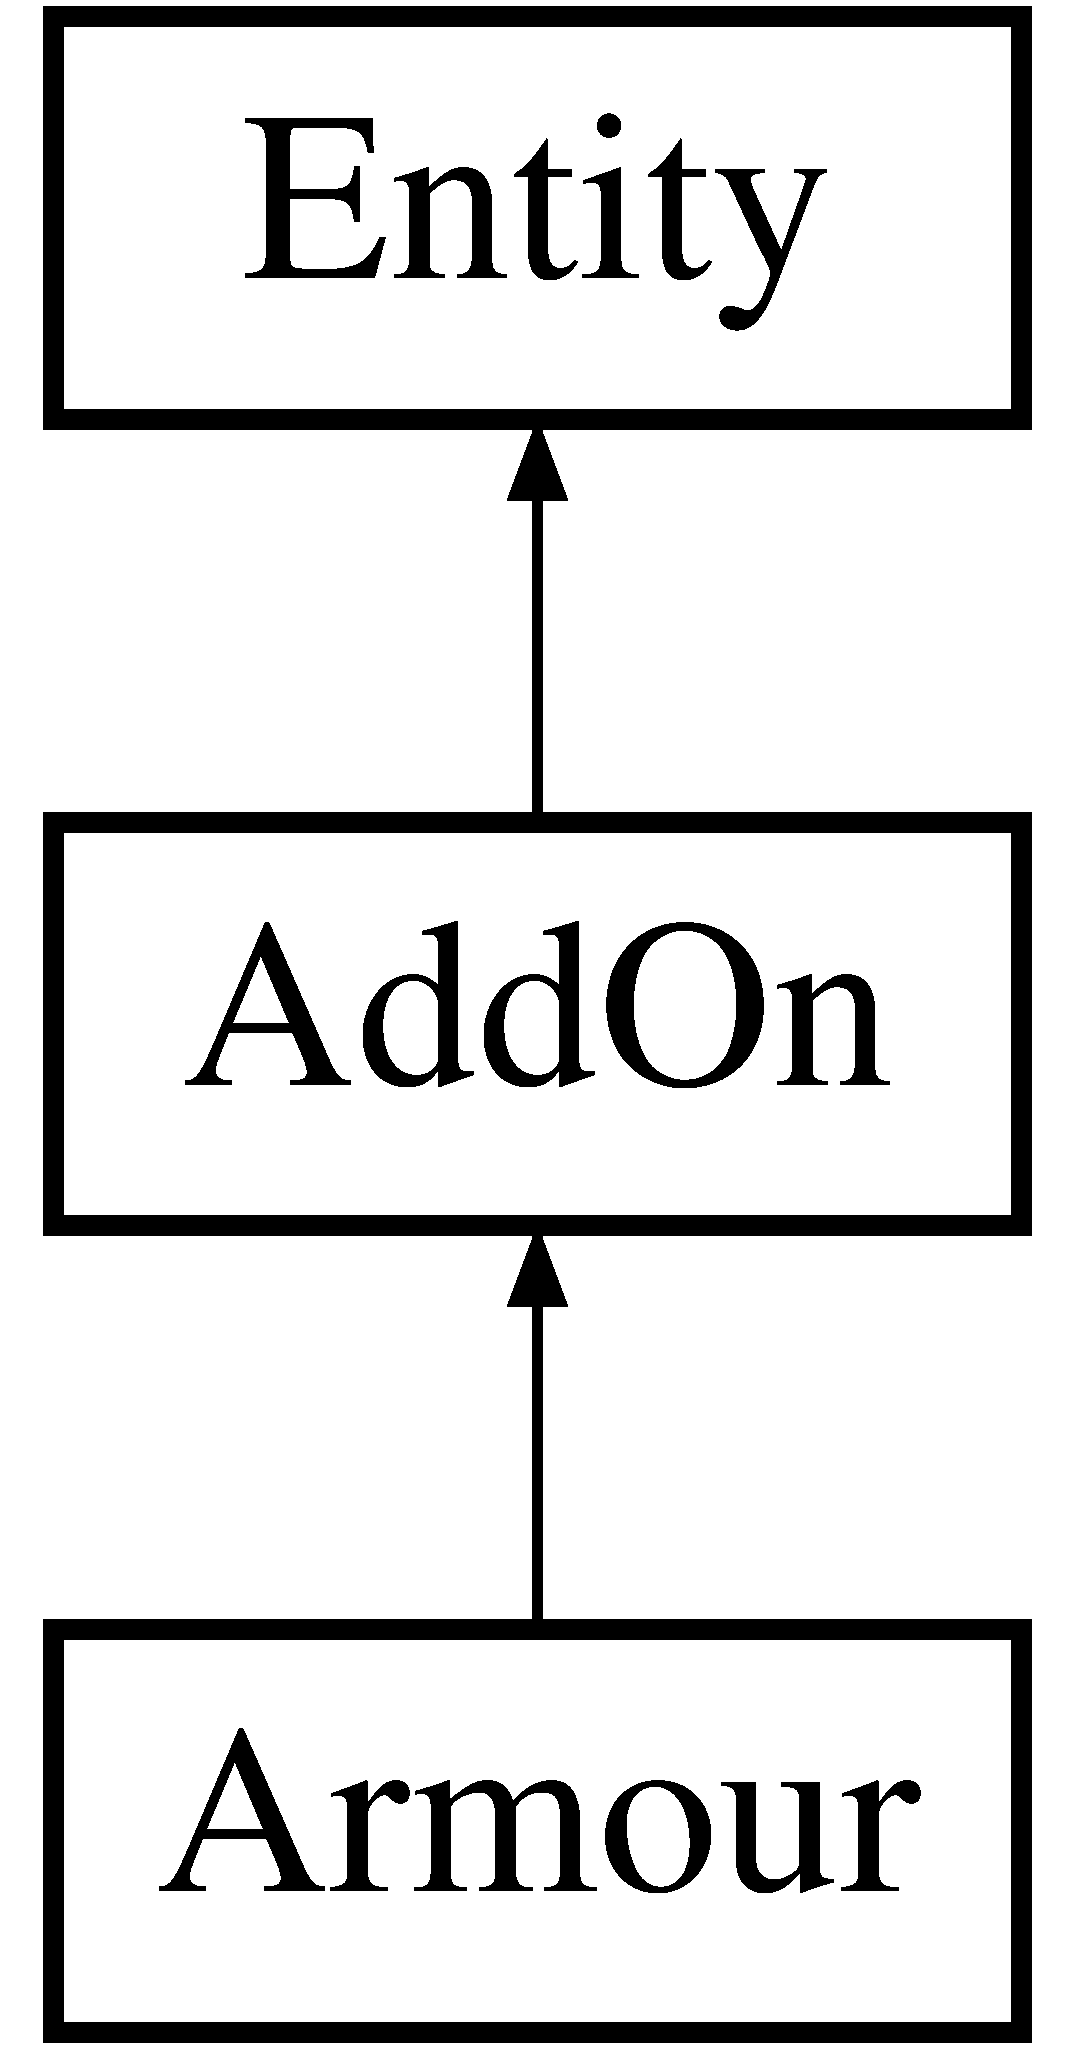
\includegraphics[height=3.000000cm]{classArmour}
\end{center}
\end{figure}
\doxysubsection*{Public Member Functions}
\begin{DoxyCompactItemize}
\item 
\mbox{\hyperlink{classArmour_a5fe1e213870c5eab65baa54bb4a3ef02}{Armour}} (int value)
\begin{DoxyCompactList}\small\item\em Instantiates an \mbox{\hyperlink{classArmour}{Armour}}. \end{DoxyCompactList}\item 
void \mbox{\hyperlink{classArmour_a7a52bd8473173c81a4ba8a6373513581}{take\+Damage}} (int damage)
\begin{DoxyCompactList}\small\item\em Decreases the entities\textquotesingle{} armour value (or health when their armour has depleted) \end{DoxyCompactList}\item 
void \mbox{\hyperlink{classArmour_acce6c768aaebaa559ac063e9d67c53b5}{deal\+Damage}} (\mbox{\hyperlink{classEntity}{Entity}} $\ast$entity)
\begin{DoxyCompactList}\small\item\em Adds to the damage \mbox{\hyperlink{classEntity}{Entity}} objects inflict. \end{DoxyCompactList}\item 
\mbox{\hyperlink{classAddOn}{Add\+On}} $\ast$ \mbox{\hyperlink{classArmour_ab200b02561ecc30c20397913a2bc9511}{clone}} ()
\begin{DoxyCompactList}\small\item\em Instantiates and returns a clone of the current \mbox{\hyperlink{classArmour}{Armour}}. \end{DoxyCompactList}\end{DoxyCompactItemize}
\doxysubsection*{Additional Inherited Members}


\doxysubsection{Detailed Description}
\mbox{\hyperlink{classArmour}{Armour}} class. 

Used to add protective armour to \mbox{\hyperlink{classEntity}{Entity}} objects. 

Definition at line \mbox{\hyperlink{Armour_8h_source_l00011}{11}} of file \mbox{\hyperlink{Armour_8h_source}{Armour.\+h}}.



\doxysubsection{Constructor \& Destructor Documentation}
\mbox{\Hypertarget{classArmour_a5fe1e213870c5eab65baa54bb4a3ef02}\label{classArmour_a5fe1e213870c5eab65baa54bb4a3ef02}} 
\index{Armour@{Armour}!Armour@{Armour}}
\index{Armour@{Armour}!Armour@{Armour}}
\doxysubsubsection{\texorpdfstring{Armour()}{Armour()}}
{\footnotesize\ttfamily Armour\+::\+Armour (\begin{DoxyParamCaption}\item[{int}]{value }\end{DoxyParamCaption})}



Instantiates an \mbox{\hyperlink{classArmour}{Armour}}. 


\begin{DoxyParams}{Parameters}
{\em value} & must be an int \\
\hline
\end{DoxyParams}


Definition at line \mbox{\hyperlink{Armour_8cpp_source_l00003}{3}} of file \mbox{\hyperlink{Armour_8cpp_source}{Armour.\+cpp}}.


\begin{DoxyCode}{0}
\DoxyCodeLine{00003 : \mbox{\hyperlink{classAddOn}{AddOn}}(value) \{\}}

\end{DoxyCode}


\doxysubsection{Member Function Documentation}
\mbox{\Hypertarget{classArmour_ab200b02561ecc30c20397913a2bc9511}\label{classArmour_ab200b02561ecc30c20397913a2bc9511}} 
\index{Armour@{Armour}!clone@{clone}}
\index{clone@{clone}!Armour@{Armour}}
\doxysubsubsection{\texorpdfstring{clone()}{clone()}}
{\footnotesize\ttfamily \mbox{\hyperlink{classAddOn}{Add\+On}} $\ast$ Armour\+::clone (\begin{DoxyParamCaption}{ }\end{DoxyParamCaption})\hspace{0.3cm}{\ttfamily [virtual]}}



Instantiates and returns a clone of the current \mbox{\hyperlink{classArmour}{Armour}}. 

Postconditions\+:
\begin{DoxyItemize}
\item Returns the clone of the current \mbox{\hyperlink{classArmour}{Armour}}
\end{DoxyItemize}

\begin{DoxyReturn}{Returns}
Armour$\ast$ The \mbox{\hyperlink{classArmour}{Armour}} clone 
\end{DoxyReturn}


Implements \mbox{\hyperlink{classAddOn}{Add\+On}}.



Definition at line \mbox{\hyperlink{Armour_8cpp_source_l00017}{17}} of file \mbox{\hyperlink{Armour_8cpp_source}{Armour.\+cpp}}.


\begin{DoxyCode}{0}
\DoxyCodeLine{00017                      \{}
\DoxyCodeLine{00018     \mbox{\hyperlink{classArmour}{Armour}}* armour = \textcolor{keyword}{new} \mbox{\hyperlink{classArmour}{Armour}}(value);}
\DoxyCodeLine{00019     \textcolor{keywordflow}{if} (\mbox{\hyperlink{classAddOn_aaf2f3af4104c7cb69ac67766790ce393}{getEntity}}() != NULL)}
\DoxyCodeLine{00020         armour-\/>\mbox{\hyperlink{classAddOn_ac9f4263e3558015fdad46adefceed197}{setEntity}}(entity-\/>clone());}
\DoxyCodeLine{00021     \textcolor{keywordflow}{return} armour;}
\DoxyCodeLine{00022 \}}

\end{DoxyCode}
\mbox{\Hypertarget{classArmour_acce6c768aaebaa559ac063e9d67c53b5}\label{classArmour_acce6c768aaebaa559ac063e9d67c53b5}} 
\index{Armour@{Armour}!dealDamage@{dealDamage}}
\index{dealDamage@{dealDamage}!Armour@{Armour}}
\doxysubsubsection{\texorpdfstring{dealDamage()}{dealDamage()}}
{\footnotesize\ttfamily void Armour\+::deal\+Damage (\begin{DoxyParamCaption}\item[{\mbox{\hyperlink{classEntity}{Entity}} $\ast$}]{entity }\end{DoxyParamCaption})\hspace{0.3cm}{\ttfamily [virtual]}}



Adds to the damage \mbox{\hyperlink{classEntity}{Entity}} objects inflict. 

Preconditions\+:
\begin{DoxyItemize}
\item entity must be an Entity$\ast$
\end{DoxyItemize}

Postconditions\+:
\begin{DoxyItemize}
\item Does nothing
\end{DoxyItemize}


\begin{DoxyParams}{Parameters}
{\em entity} & must be an Entity$\ast$ \\
\hline
\end{DoxyParams}
\begin{DoxyReturn}{Returns}
void 
\end{DoxyReturn}


Implements \mbox{\hyperlink{classAddOn}{Add\+On}}.



Definition at line \mbox{\hyperlink{Armour_8cpp_source_l00013}{13}} of file \mbox{\hyperlink{Armour_8cpp_source}{Armour.\+cpp}}.


\begin{DoxyCode}{0}
\DoxyCodeLine{00013                                       \{}
\DoxyCodeLine{00014     this-\/>entity-\/>dealDamage(entity);}
\DoxyCodeLine{00015 \}}

\end{DoxyCode}
\mbox{\Hypertarget{classArmour_a7a52bd8473173c81a4ba8a6373513581}\label{classArmour_a7a52bd8473173c81a4ba8a6373513581}} 
\index{Armour@{Armour}!takeDamage@{takeDamage}}
\index{takeDamage@{takeDamage}!Armour@{Armour}}
\doxysubsubsection{\texorpdfstring{takeDamage()}{takeDamage()}}
{\footnotesize\ttfamily void Armour\+::take\+Damage (\begin{DoxyParamCaption}\item[{int}]{damage }\end{DoxyParamCaption})\hspace{0.3cm}{\ttfamily [virtual]}}



Decreases the entities\textquotesingle{} armour value (or health when their armour has depleted) 

Preconditions\+:
\begin{DoxyItemize}
\item damage must be an int
\end{DoxyItemize}

Postconditions\+:
\begin{DoxyItemize}
\item Decreases the entities\textquotesingle{} armour value (or health when their armour has diminished) by the passed in value
\end{DoxyItemize}


\begin{DoxyParams}{Parameters}
{\em damage} & must be an int \\
\hline
\end{DoxyParams}
\begin{DoxyReturn}{Returns}
void 
\end{DoxyReturn}


Implements \mbox{\hyperlink{classAddOn}{Add\+On}}.



Definition at line \mbox{\hyperlink{Armour_8cpp_source_l00005}{5}} of file \mbox{\hyperlink{Armour_8cpp_source}{Armour.\+cpp}}.


\begin{DoxyCode}{0}
\DoxyCodeLine{00005                                   \{}
\DoxyCodeLine{00006     \textcolor{keywordflow}{if} (value > 0) \{}
\DoxyCodeLine{00007         value -\/= damage;}
\DoxyCodeLine{00008     \} \textcolor{keywordflow}{else} \{}
\DoxyCodeLine{00009         entity-\/>takeDamage(damage);}
\DoxyCodeLine{00010     \}}
\DoxyCodeLine{00011 \}}

\end{DoxyCode}


The documentation for this class was generated from the following files\+:\begin{DoxyCompactItemize}
\item 
Armour.\+h\item 
Armour.\+cpp\end{DoxyCompactItemize}

\hypertarget{classCloudy}{}\doxysection{Cloudy Class Reference}
\label{classCloudy}\index{Cloudy@{Cloudy}}
Inheritance diagram for Cloudy\+:\begin{figure}[H]
\begin{center}
\leavevmode
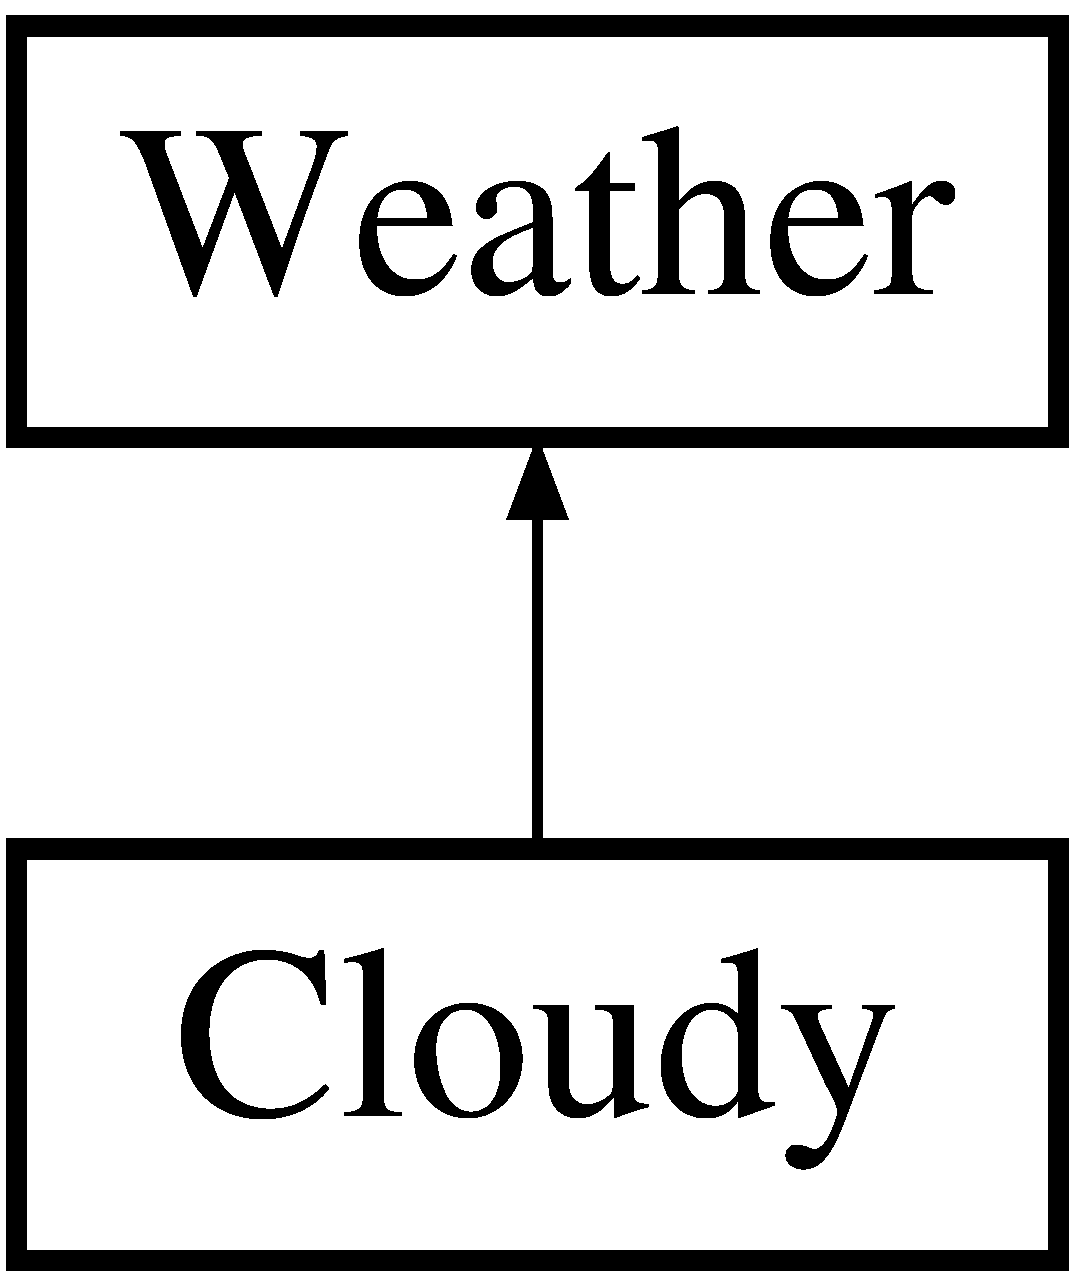
\includegraphics[height=2.000000cm]{classCloudy}
\end{center}
\end{figure}
\doxysubsection*{Public Member Functions}
\begin{DoxyCompactItemize}
\item 
<<<<<<< HEAD
<<<<<<< HEAD
\mbox{\Hypertarget{classCloudy_a343d3f7df85d665400b9c945e1d70e9f}\label{classCloudy_a343d3f7df85d665400b9c945e1d70e9f}} 
\hyperlink{classCloudy_a343d3f7df85d665400b9c945e1d70e9f}{Cloudy} ()
\begin{DoxyCompactList}\small\item\em Instantiates the \hyperlink{classCloudy}{Cloudy} object of the state pattern. \end{DoxyCompactList}\item 
std\+::string \hyperlink{classCloudy_a859714ec61c789dc12ed5447fd3692ac}{get\+Weather} ()
\begin{DoxyCompactList}\small\item\em Returns string which tels us the weather. \end{DoxyCompactList}\item 
void \hyperlink{classCloudy_aa01a409307657c9a7cad11a6f93456fd}{handle\+Change} (\hyperlink{classKeyPoint}{Key\+Point} $\ast$k)
\begin{DoxyCompactList}\small\item\em Will change the current state of the weather inside the specific keypoint. \end{DoxyCompactList}\end{DoxyCompactItemize}
\subsection*{Additional Inherited Members}
=======
\mbox{\hyperlink{classCloudy_a343d3f7df85d665400b9c945e1d70e9f}{Cloudy}} ()
\begin{DoxyCompactList}\small\item\em Instantiates the \mbox{\hyperlink{classCloudy}{Cloudy}} object of the state pattern. \end{DoxyCompactList}\item 
std\+::string \mbox{\hyperlink{classCloudy_a859714ec61c789dc12ed5447fd3692ac}{get\+Weather}} ()
\begin{DoxyCompactList}\small\item\em Returns string which tels us the weather. \end{DoxyCompactList}\item 
=======
\mbox{\hyperlink{classCloudy_a343d3f7df85d665400b9c945e1d70e9f}{Cloudy}} ()
\begin{DoxyCompactList}\small\item\em Instantiates the \mbox{\hyperlink{classCloudy}{Cloudy}} object of the state pattern. \end{DoxyCompactList}\item 
std\+::string \mbox{\hyperlink{classCloudy_a859714ec61c789dc12ed5447fd3692ac}{get\+Weather}} ()
\begin{DoxyCompactList}\small\item\em Returns string which tels us the weather. \end{DoxyCompactList}\item 
>>>>>>> 7be49738cebc0ced3357f2ce74f6fda2ea0b3d5e
void \mbox{\hyperlink{classCloudy_aa01a409307657c9a7cad11a6f93456fd}{handle\+Change}} (\mbox{\hyperlink{classKeyPoint}{Key\+Point}} $\ast$k)
\begin{DoxyCompactList}\small\item\em Will change the current state of the weather inside the specific keypoint. \end{DoxyCompactList}\item 
\mbox{\hyperlink{classWeather}{Weather}} $\ast$ \mbox{\hyperlink{classCloudy_ab55ddd71864e27bb1f02f0af8d44a206}{clone}} ()
\begin{DoxyCompactList}\small\item\em Returns a clone of the \mbox{\hyperlink{classCloudy}{Cloudy}} object. \end{DoxyCompactList}\end{DoxyCompactItemize}
\doxysubsection*{Additional Inherited Members}
<<<<<<< HEAD
>>>>>>> 7be49738cebc0ced3357f2ce74f6fda2ea0b3d5e
=======
>>>>>>> 7be49738cebc0ced3357f2ce74f6fda2ea0b3d5e


\doxysubsection{Detailed Description}


<<<<<<< HEAD
<<<<<<< HEAD
Definition at line 6 of file Cloudy.\+h.



\subsection{Member Function Documentation}
\mbox{\Hypertarget{classCloudy_a859714ec61c789dc12ed5447fd3692ac}\label{classCloudy_a859714ec61c789dc12ed5447fd3692ac}} 
\index{Cloudy@{Cloudy}!get\+Weather@{get\+Weather}}
\index{get\+Weather@{get\+Weather}!Cloudy@{Cloudy}}
\subsubsection{\texorpdfstring{get\+Weather()}{getWeather()}}
=======
Definition at line \mbox{\hyperlink{Cloudy_8h_source_l00006}{6}} of file \mbox{\hyperlink{Cloudy_8h_source}{Cloudy.\+h}}.



=======
Definition at line \mbox{\hyperlink{Cloudy_8h_source_l00006}{6}} of file \mbox{\hyperlink{Cloudy_8h_source}{Cloudy.\+h}}.



>>>>>>> 7be49738cebc0ced3357f2ce74f6fda2ea0b3d5e
\doxysubsection{Constructor \& Destructor Documentation}
\mbox{\Hypertarget{classCloudy_a343d3f7df85d665400b9c945e1d70e9f}\label{classCloudy_a343d3f7df85d665400b9c945e1d70e9f}} 
\index{Cloudy@{Cloudy}!Cloudy@{Cloudy}}
\index{Cloudy@{Cloudy}!Cloudy@{Cloudy}}
\doxysubsubsection{\texorpdfstring{Cloudy()}{Cloudy()}}
{\footnotesize\ttfamily Cloudy\+::\+Cloudy (\begin{DoxyParamCaption}{ }\end{DoxyParamCaption})}



Instantiates the \mbox{\hyperlink{classCloudy}{Cloudy}} object of the state pattern. 



Definition at line \mbox{\hyperlink{Cloudy_8cpp_source_l00004}{4}} of file \mbox{\hyperlink{Cloudy_8cpp_source}{Cloudy.\+cpp}}.


\begin{DoxyCode}{0}
\DoxyCodeLine{00004               : \mbox{\hyperlink{classWeather_aa404c94fec05b825454a7309827767c6}{Weather}}() \{}
\DoxyCodeLine{00005     this-\/>multiplier = 0.75;}
\DoxyCodeLine{00006 \}}

\end{DoxyCode}


\doxysubsection{Member Function Documentation}
\mbox{\Hypertarget{classCloudy_ab55ddd71864e27bb1f02f0af8d44a206}\label{classCloudy_ab55ddd71864e27bb1f02f0af8d44a206}} 
\index{Cloudy@{Cloudy}!clone@{clone}}
\index{clone@{clone}!Cloudy@{Cloudy}}
\doxysubsubsection{\texorpdfstring{clone()}{clone()}}
{\footnotesize\ttfamily \mbox{\hyperlink{classWeather}{Weather}} $\ast$ Cloudy\+::clone (\begin{DoxyParamCaption}{ }\end{DoxyParamCaption})\hspace{0.3cm}{\ttfamily [virtual]}}



Returns a clone of the \mbox{\hyperlink{classCloudy}{Cloudy}} object. 

\begin{DoxyReturn}{Returns}
Weather$\ast$ Clone of cloudy object 
\end{DoxyReturn}


Implements \mbox{\hyperlink{classWeather}{Weather}}.



Definition at line \mbox{\hyperlink{Cloudy_8cpp_source_l00017}{17}} of file \mbox{\hyperlink{Cloudy_8cpp_source}{Cloudy.\+cpp}}.


\begin{DoxyCode}{0}
\DoxyCodeLine{00017                        \{}
\DoxyCodeLine{00018     \textcolor{keywordflow}{return} \textcolor{keyword}{new} \mbox{\hyperlink{classCloudy_a343d3f7df85d665400b9c945e1d70e9f}{Cloudy}}();}
\DoxyCodeLine{00019 \}}

\end{DoxyCode}
\mbox{\Hypertarget{classCloudy_a859714ec61c789dc12ed5447fd3692ac}\label{classCloudy_a859714ec61c789dc12ed5447fd3692ac}} 
\index{Cloudy@{Cloudy}!getWeather@{getWeather}}
\index{getWeather@{getWeather}!Cloudy@{Cloudy}}
\doxysubsubsection{\texorpdfstring{getWeather()}{getWeather()}}
<<<<<<< HEAD
>>>>>>> 7be49738cebc0ced3357f2ce74f6fda2ea0b3d5e
=======
>>>>>>> 7be49738cebc0ced3357f2ce74f6fda2ea0b3d5e
{\footnotesize\ttfamily std\+::string Cloudy\+::get\+Weather (\begin{DoxyParamCaption}{ }\end{DoxyParamCaption})\hspace{0.3cm}{\ttfamily [virtual]}}



Returns string which tels us the weather. 

Postconditions\+:
\begin{DoxyItemize}
\item Returns the wether of ths current state
\end{DoxyItemize}

\begin{DoxyReturn}{Returns}
std\+::string which is the current state 
\end{DoxyReturn}


<<<<<<< HEAD
<<<<<<< HEAD
Implements \hyperlink{classWeather_ad0a29227308b87e98808cdff52232df3}{Weather}.



Definition at line 8 of file Cloudy.\+cpp.


\begin{DoxyCode}
8                              \{
9     \textcolor{keywordflow}{return} \textcolor{stringliteral}{"Cloudy"};
10 \}
\end{DoxyCode}
\mbox{\Hypertarget{classCloudy_aa01a409307657c9a7cad11a6f93456fd}\label{classCloudy_aa01a409307657c9a7cad11a6f93456fd}} 
\index{Cloudy@{Cloudy}!handle\+Change@{handle\+Change}}
\index{handle\+Change@{handle\+Change}!Cloudy@{Cloudy}}
\subsubsection{\texorpdfstring{handle\+Change()}{handleChange()}}
{\footnotesize\ttfamily void Cloudy\+::handle\+Change (\begin{DoxyParamCaption}\item[{\hyperlink{classKeyPoint}{Key\+Point} $\ast$}]{k }\end{DoxyParamCaption})\hspace{0.3cm}{\ttfamily [virtual]}}
=======
Implements \mbox{\hyperlink{classWeather}{Weather}}.



=======
Implements \mbox{\hyperlink{classWeather}{Weather}}.



>>>>>>> 7be49738cebc0ced3357f2ce74f6fda2ea0b3d5e
Definition at line \mbox{\hyperlink{Cloudy_8cpp_source_l00008}{8}} of file \mbox{\hyperlink{Cloudy_8cpp_source}{Cloudy.\+cpp}}.


\begin{DoxyCode}{0}
\DoxyCodeLine{00008                              \{}
\DoxyCodeLine{00009     \textcolor{keywordflow}{return} \textcolor{stringliteral}{"{}Cloudy"{}};}
\DoxyCodeLine{00010 \}}

\end{DoxyCode}
\mbox{\Hypertarget{classCloudy_aa01a409307657c9a7cad11a6f93456fd}\label{classCloudy_aa01a409307657c9a7cad11a6f93456fd}} 
\index{Cloudy@{Cloudy}!handleChange@{handleChange}}
\index{handleChange@{handleChange}!Cloudy@{Cloudy}}
\doxysubsubsection{\texorpdfstring{handleChange()}{handleChange()}}
{\footnotesize\ttfamily void Cloudy\+::handle\+Change (\begin{DoxyParamCaption}\item[{\mbox{\hyperlink{classKeyPoint}{Key\+Point}} $\ast$}]{k }\end{DoxyParamCaption})\hspace{0.3cm}{\ttfamily [virtual]}}
<<<<<<< HEAD
>>>>>>> 7be49738cebc0ced3357f2ce74f6fda2ea0b3d5e
=======
>>>>>>> 7be49738cebc0ced3357f2ce74f6fda2ea0b3d5e



Will change the current state of the weather inside the specific keypoint. 

Preconditions\+:
\begin{DoxyItemize}
\item k must be a Key\+Point$\ast$
\end{DoxyItemize}

Postconditions\+:
\begin{DoxyItemize}
\item Changes the current weather to the next one in the state pattern (\mbox{\hyperlink{classRainy}{Rainy}})
\end{DoxyItemize}


\begin{DoxyParams}{Parameters}
{\em k} & must be a Key\+Point$\ast$ \\
\hline
\end{DoxyParams}
\begin{DoxyReturn}{Returns}
void 
\end{DoxyReturn}


<<<<<<< HEAD
<<<<<<< HEAD
Implements \hyperlink{classWeather_afc84c48c326fc967915833e689bfa40c}{Weather}.



Definition at line 12 of file Cloudy.\+cpp.


\begin{DoxyCode}
12                                      \{
13     \hyperlink{classRainy}{Rainy}* newWeather = \textcolor{keyword}{new} \hyperlink{classRainy}{Rainy}();
14     k->\hyperlink{classKeyPoint_a5c4b9314440a00fca7ab4d82ea4693a5}{setWeather}(newWeather);
15 \}
=======
Implements \mbox{\hyperlink{classWeather}{Weather}}.



=======
Implements \mbox{\hyperlink{classWeather}{Weather}}.



>>>>>>> 7be49738cebc0ced3357f2ce74f6fda2ea0b3d5e
Definition at line \mbox{\hyperlink{Cloudy_8cpp_source_l00012}{12}} of file \mbox{\hyperlink{Cloudy_8cpp_source}{Cloudy.\+cpp}}.


\begin{DoxyCode}{0}
\DoxyCodeLine{00012                                      \{}
\DoxyCodeLine{00013     \mbox{\hyperlink{classRainy}{Rainy}}* newWeather = \textcolor{keyword}{new} \mbox{\hyperlink{classRainy}{Rainy}}();}
\DoxyCodeLine{00014     k-\/>\mbox{\hyperlink{classKeyPoint_a5c4b9314440a00fca7ab4d82ea4693a5}{setWeather}}(newWeather);}
\DoxyCodeLine{00015 \}}

<<<<<<< HEAD
>>>>>>> 7be49738cebc0ced3357f2ce74f6fda2ea0b3d5e
=======
>>>>>>> 7be49738cebc0ced3357f2ce74f6fda2ea0b3d5e
\end{DoxyCode}


The documentation for this class was generated from the following files\+:\begin{DoxyCompactItemize}
\item 
Cloudy.\+h\item 
Cloudy.\+cpp\end{DoxyCompactItemize}

\hypertarget{classCommandCenter}{}\doxysection{Command\+Center Class Reference}
\label{classCommandCenter}\index{CommandCenter@{CommandCenter}}


\mbox{\hyperlink{classCommandCenter}{Command\+Center}} class.  




{\ttfamily \#include $<$Command\+Center.\+h$>$}

\doxysubsection*{Public Member Functions}
\begin{DoxyCompactItemize}
\item 
\mbox{\Hypertarget{classCommandCenter_a3fc4f465f7c24d9c9158baf0e03ac571}\label{classCommandCenter_a3fc4f465f7c24d9c9158baf0e03ac571}} 
\mbox{\hyperlink{classCommandCenter_a3fc4f465f7c24d9c9158baf0e03ac571}{Command\+Center}} ()
\begin{DoxyCompactList}\small\item\em Instantiates the \mbox{\hyperlink{classCommandCenter}{Command\+Center}}. \end{DoxyCompactList}\item 
void \mbox{\hyperlink{classCommandCenter_a1aee52be7351e2e2c78c8d239d31cff0}{update}} (\mbox{\hyperlink{classKeyPoint}{Key\+Point}} $\ast$key\+Point)
\begin{DoxyCompactList}\small\item\em Updates the command center\textquotesingle{}s keypoint state. \end{DoxyCompactList}\item 
\mbox{\Hypertarget{classCommandCenter_aef666a19f24fd089edd089e4b2cb9542}\label{classCommandCenter_aef666a19f24fd089edd089e4b2cb9542}} 
\mbox{\hyperlink{classCommandCenter}{Command\+Center}} $\ast$ {\bfseries clone} ()
\end{DoxyCompactItemize}


\doxysubsection{Detailed Description}
\mbox{\hyperlink{classCommandCenter}{Command\+Center}} class. 

Used to observe the entities and weather at the Keypoint objects. 

Definition at line 9 of file Command\+Center.\+h.



\doxysubsection{Member Function Documentation}
\mbox{\Hypertarget{classCommandCenter_a1aee52be7351e2e2c78c8d239d31cff0}\label{classCommandCenter_a1aee52be7351e2e2c78c8d239d31cff0}} 
\index{CommandCenter@{CommandCenter}!update@{update}}
\index{update@{update}!CommandCenter@{CommandCenter}}
\doxysubsubsection{\texorpdfstring{update()}{update()}}
{\footnotesize\ttfamily void Command\+Center\+::update (\begin{DoxyParamCaption}\item[{\mbox{\hyperlink{classKeyPoint}{Key\+Point}} $\ast$}]{key\+Point }\end{DoxyParamCaption})}



Updates the command center\textquotesingle{}s keypoint state. 

Preconditions\+:
\begin{DoxyItemize}
\item key\+Point must be a Key\+Point$\ast$
\end{DoxyItemize}

Postconditions\+:
\begin{DoxyItemize}
\item Updates the command centers\textquotesingle{} keypoint state with the passed in key\+Point
\end{DoxyItemize}


\begin{DoxyParams}{Parameters}
{\em key\+Point} & must be a Key\+Point$\ast$ \\
\hline
\end{DoxyParams}
\begin{DoxyReturn}{Returns}
void 
\end{DoxyReturn}


Definition at line 8 of file Command\+Center.\+cpp.


\begin{DoxyCode}{0}
\DoxyCodeLine{8                                              \{}
\DoxyCodeLine{9     \textcolor{comment}{// TODO -\/ implement CommandCenter::update}}
\DoxyCodeLine{10     \textcolor{keywordflow}{throw} \textcolor{stringliteral}{"Not yet implemented"};}
\DoxyCodeLine{11 \}}

\end{DoxyCode}


The documentation for this class was generated from the following files\+:\begin{DoxyCompactItemize}
\item 
Command\+Center.\+h\item 
Command\+Center.\+cpp\end{DoxyCompactItemize}

\hypertarget{classCountry}{}\section{Country Class Reference}
\label{classCountry}\index{Country@{Country}}
\subsection*{Public Member Functions}
\begin{DoxyCompactItemize}
\item 
\mbox{\Hypertarget{classCountry_a4cba457856775a13a17dfcb11a77e224}\label{classCountry_a4cba457856775a13a17dfcb11a77e224}} 
\hyperlink{classCountry_a4cba457856775a13a17dfcb11a77e224}{Country} ()
\begin{DoxyCompactList}\small\item\em Instantiates the \hyperlink{classCountry}{Country}. \end{DoxyCompactList}\item 
\hyperlink{classCountry}{Country} $\ast$ \hyperlink{classCountry_a82562b18230bbeceb22b13c0ab046a1c}{clone} ()
\begin{DoxyCompactList}\small\item\em Instantiates and returns a clone of the current \hyperlink{classCountry}{Country}. \end{DoxyCompactList}\item 
void \hyperlink{classCountry_ae4773ebfffe4f9d2d2db1b54181b67ab}{set\+Name} (std\+::string name)
\begin{DoxyCompactList}\small\item\em Set the name of the country. \end{DoxyCompactList}\item 
void \hyperlink{classCountry_a35ecd0419e6a6eaf358889527c280d82}{set\+ID} (int id)
\begin{DoxyCompactList}\small\item\em Set the if of the country. \end{DoxyCompactList}\item 
std\+::string \hyperlink{classCountry_af86e64cecec9c266dbf284329ab072f3}{get\+Name} () const
\begin{DoxyCompactList}\small\item\em Get the name of the country. \end{DoxyCompactList}\item 
int \hyperlink{classCountry_abb770576662c91a71c01cf078b98c0af}{get\+ID} () const
\begin{DoxyCompactList}\small\item\em Get the id of the country. \end{DoxyCompactList}\end{DoxyCompactItemize}


\subsection{Detailed Description}


Definition at line 5 of file Country.\+h.



\subsection{Member Function Documentation}
\mbox{\Hypertarget{classCountry_a82562b18230bbeceb22b13c0ab046a1c}\label{classCountry_a82562b18230bbeceb22b13c0ab046a1c}} 
\index{Country@{Country}!clone@{clone}}
\index{clone@{clone}!Country@{Country}}
\subsubsection{\texorpdfstring{clone()}{clone()}}
{\footnotesize\ttfamily \hyperlink{classCountry}{Country} $\ast$ Country\+::clone (\begin{DoxyParamCaption}{ }\end{DoxyParamCaption})}



Instantiates and returns a clone of the current \hyperlink{classCountry}{Country}. 

Postconditions\+:
\begin{DoxyItemize}
\item Returns the clone of the current \hyperlink{classCountry}{Country}
\end{DoxyItemize}

\begin{DoxyReturn}{Returns}
Country$\ast$ The country clone 
\end{DoxyReturn}


Definition at line 9 of file Country.\+cpp.


\begin{DoxyCode}
9                        \{
10     
11     \hyperlink{classCountry}{Country}* countryClone = \textcolor{keyword}{new} \hyperlink{classCountry_a4cba457856775a13a17dfcb11a77e224}{Country}();
12     countryClone->\hyperlink{classCountry_a35ecd0419e6a6eaf358889527c280d82}{setID}(this->\textcolor{keywordtype}{id});
13     countryClone->\hyperlink{classCountry_ae4773ebfffe4f9d2d2db1b54181b67ab}{setName}(this->name);
14 
15     \textcolor{keywordflow}{return} countryClone;
16 \}
\end{DoxyCode}
\mbox{\Hypertarget{classCountry_abb770576662c91a71c01cf078b98c0af}\label{classCountry_abb770576662c91a71c01cf078b98c0af}} 
\index{Country@{Country}!get\+ID@{get\+ID}}
\index{get\+ID@{get\+ID}!Country@{Country}}
\subsubsection{\texorpdfstring{get\+I\+D()}{getID()}}
{\footnotesize\ttfamily int Country\+::get\+ID (\begin{DoxyParamCaption}{ }\end{DoxyParamCaption}) const}



Get the id of the country. 

Post\+Conditions\+:
\begin{DoxyItemize}
\item return the id the id of the country
\end{DoxyItemize}

\begin{DoxyReturn}{Returns}
int 
\end{DoxyReturn}


Definition at line 30 of file Country.\+cpp.


\begin{DoxyCode}
30                         \{
31     \textcolor{keywordflow}{return} this->id;
32 \}
\end{DoxyCode}
\mbox{\Hypertarget{classCountry_af86e64cecec9c266dbf284329ab072f3}\label{classCountry_af86e64cecec9c266dbf284329ab072f3}} 
\index{Country@{Country}!get\+Name@{get\+Name}}
\index{get\+Name@{get\+Name}!Country@{Country}}
\subsubsection{\texorpdfstring{get\+Name()}{getName()}}
{\footnotesize\ttfamily string Country\+::get\+Name (\begin{DoxyParamCaption}{ }\end{DoxyParamCaption}) const}



Get the name of the country. 

Post\+Conditions\+:
\begin{DoxyItemize}
\item Return the name of the country
\end{DoxyItemize}

\begin{DoxyReturn}{Returns}
string 
\end{DoxyReturn}


Definition at line 26 of file Country.\+cpp.


\begin{DoxyCode}
26                              \{
27     \textcolor{keywordflow}{return} this->name;
28 \}
\end{DoxyCode}
\mbox{\Hypertarget{classCountry_a35ecd0419e6a6eaf358889527c280d82}\label{classCountry_a35ecd0419e6a6eaf358889527c280d82}} 
\index{Country@{Country}!set\+ID@{set\+ID}}
\index{set\+ID@{set\+ID}!Country@{Country}}
\subsubsection{\texorpdfstring{set\+I\+D()}{setID()}}
{\footnotesize\ttfamily void Country\+::set\+ID (\begin{DoxyParamCaption}\item[{int}]{id }\end{DoxyParamCaption})}



Set the if of the country. 

Precondition\+:
\begin{DoxyItemize}
\item The variale if is type of int
\end{DoxyItemize}

Preconditions\+:
\begin{DoxyItemize}
\item The variable id is set the the passed in parameter 
\begin{DoxyParams}{Parameters}
{\em id} & \\
\hline
\end{DoxyParams}

\end{DoxyItemize}

Definition at line 18 of file Country.\+cpp.


\begin{DoxyCode}
18                          \{
19     this->\textcolor{keywordtype}{id} = id;
20 \}
\end{DoxyCode}
\mbox{\Hypertarget{classCountry_ae4773ebfffe4f9d2d2db1b54181b67ab}\label{classCountry_ae4773ebfffe4f9d2d2db1b54181b67ab}} 
\index{Country@{Country}!set\+Name@{set\+Name}}
\index{set\+Name@{set\+Name}!Country@{Country}}
\subsubsection{\texorpdfstring{set\+Name()}{setName()}}
{\footnotesize\ttfamily void Country\+::set\+Name (\begin{DoxyParamCaption}\item[{std\+::string}]{name }\end{DoxyParamCaption})}



Set the name of the country. 

Precondition\+:
\begin{DoxyItemize}
\item The variale name is type of string
\end{DoxyItemize}

Preconditions\+:
\begin{DoxyItemize}
\item The variable name is set the the passed in parameter 
\begin{DoxyParams}{Parameters}
{\em name} & \\
\hline
\end{DoxyParams}

\end{DoxyItemize}

Definition at line 22 of file Country.\+cpp.


\begin{DoxyCode}
22                                 \{
23     this->name = name;
24 \}
\end{DoxyCode}


The documentation for this class was generated from the following files\+:\begin{DoxyCompactItemize}
\item 
Country.\+h\item 
Country.\+cpp\end{DoxyCompactItemize}

\hypertarget{classDefensive}{}\doxysection{Defensive Class Reference}
\label{classDefensive}\index{Defensive@{Defensive}}
Inheritance diagram for Defensive\+:\begin{figure}[H]
\begin{center}
\leavevmode
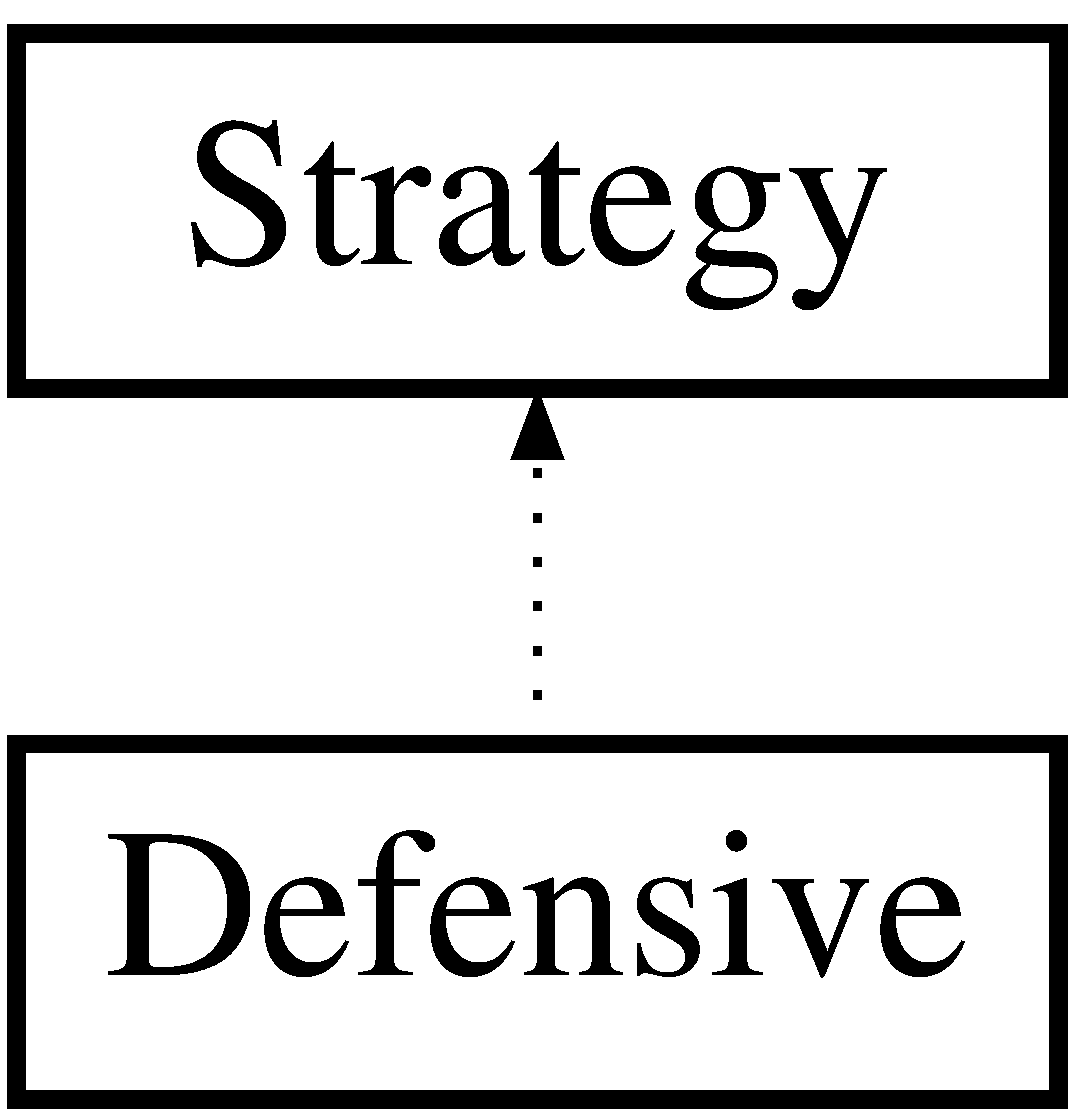
\includegraphics[height=2.000000cm]{classDefensive}
\end{center}
\end{figure}
\doxysubsection*{Public Member Functions}
\begin{DoxyCompactItemize}
\item 
void \mbox{\hyperlink{classDefensive_ad824897b2075d2184612ab6efcdd8367}{perform\+Strat}} (\mbox{\hyperlink{classKeyPoint}{Key\+Point}} $\ast$key\+Point)
\begin{DoxyCompactList}\small\item\em This function will perform an \mbox{\hyperlink{classDefensive}{Defensive}} strategy. \end{DoxyCompactList}\end{DoxyCompactItemize}
\doxysubsection*{Additional Inherited Members}


\doxysubsection{Detailed Description}


Definition at line 6 of file Defensive.\+h.



\doxysubsection{Member Function Documentation}
\mbox{\Hypertarget{classDefensive_ad824897b2075d2184612ab6efcdd8367}\label{classDefensive_ad824897b2075d2184612ab6efcdd8367}} 
\index{Defensive@{Defensive}!performStrat@{performStrat}}
\index{performStrat@{performStrat}!Defensive@{Defensive}}
\doxysubsubsection{\texorpdfstring{performStrat()}{performStrat()}}
{\footnotesize\ttfamily void Defensive\+::perform\+Strat (\begin{DoxyParamCaption}\item[{\mbox{\hyperlink{classKeyPoint}{Key\+Point}} $\ast$}]{key\+Point }\end{DoxyParamCaption})\hspace{0.3cm}{\ttfamily [virtual]}}



This function will perform an \mbox{\hyperlink{classDefensive}{Defensive}} strategy. 

\begin{DoxyAuthor}{Author}
Antwi-\/\+Antwi
\end{DoxyAuthor}

\begin{DoxyParams}{Parameters}
{\em key\+Point} & an \mbox{\hyperlink{classDefensive}{Defensive}} strategy will then be performed at this specific keypoint\\
\hline
\end{DoxyParams}
\begin{DoxyReturn}{Returns}
void The function will return a void 
\end{DoxyReturn}


Implements \mbox{\hyperlink{classStrategy_ada170bd47bc6f11ac02d7df2b366387b}{Strategy}}.



Definition at line 8 of file Defensive.\+cpp.


\begin{DoxyCode}{0}
\DoxyCodeLine{8                                                \{}
\DoxyCodeLine{9     \textcolor{comment}{// TODO -\/ implement Defensive::performStrat}}
\DoxyCodeLine{10     \textcolor{keywordflow}{throw} \textcolor{stringliteral}{"Not yet implemented"};}
\DoxyCodeLine{11 \}}

\end{DoxyCode}


The documentation for this class was generated from the following files\+:\begin{DoxyCompactItemize}
\item 
Defensive.\+h\item 
Defensive.\+cpp\end{DoxyCompactItemize}

\hypertarget{classEntity}{}\doxysection{Entity Class Reference}
\label{classEntity}\index{Entity@{Entity}}


\mbox{\hyperlink{classEntity}{Entity}} class.  




{\ttfamily \#include $<$Entity.\+h$>$}

Inheritance diagram for Entity\+:\begin{figure}[H]
\begin{center}
\leavevmode
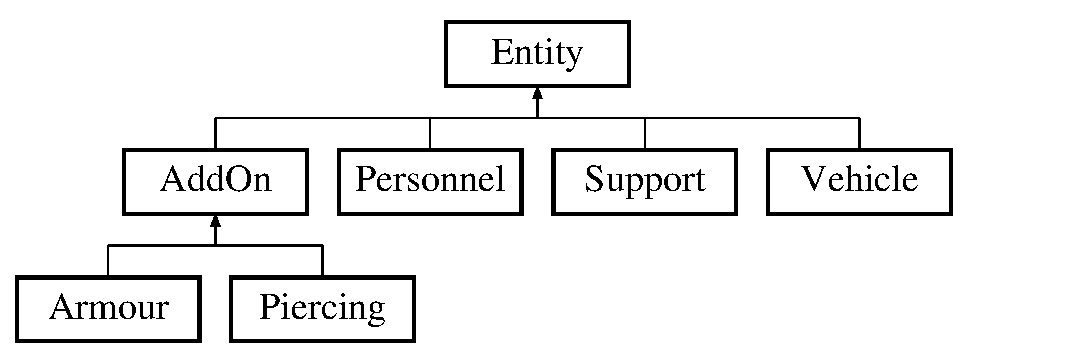
\includegraphics[height=3.000000cm]{classEntity}
\end{center}
\end{figure}
\doxysubsection*{Public Member Functions}
\begin{DoxyCompactItemize}
\item 
\mbox{\hyperlink{classEntity_a980f368aa07ce358583982821533a54a}{Entity}} ()
\begin{DoxyCompactList}\small\item\em Instantiates the entity. \end{DoxyCompactList}\item 
\mbox{\hyperlink{classEntity_a68e832f69650ee80b83228a038eb66f0}{Entity}} (\mbox{\hyperlink{classType}{Type}} $\ast$type, int health, int damage)
\begin{DoxyCompactList}\small\item\em Instantiates the entity. \end{DoxyCompactList}\item 
\mbox{\hyperlink{classType}{Type}} $\ast$ \mbox{\hyperlink{classEntity_a3a9c9e298bfc47b726a2d9ce44dd7464}{get\+Type}} ()
\begin{DoxyCompactList}\small\item\em Returns entities type state. \end{DoxyCompactList}\item 
void \mbox{\hyperlink{classEntity_a5d04ce64c9ca214900422865e298e36c}{set\+Type}} (\mbox{\hyperlink{classType}{Type}} $\ast$type)
\begin{DoxyCompactList}\small\item\em Sets the entities type state. \end{DoxyCompactList}\item 
\mbox{\hyperlink{classAlliance}{Alliance}} $\ast$ \mbox{\hyperlink{classEntity_aa101047a4bc312b697b65b4c3a39ffc5}{get\+Alliance}} ()
\begin{DoxyCompactList}\small\item\em Returns entities alliance. \end{DoxyCompactList}\item 
void \mbox{\hyperlink{classEntity_af804dcaa600e770cf0e2b4537f6fba23}{set\+Alliance}} (\mbox{\hyperlink{classAlliance}{Alliance}} $\ast$alliance)
\begin{DoxyCompactList}\small\item\em Sets the entities alliance. \end{DoxyCompactList}\item 
int \mbox{\hyperlink{classEntity_a2b0140ae8c77c0e3654b070ee3c7fe57}{get\+Health}} ()
\begin{DoxyCompactList}\small\item\em Returns entities health. \end{DoxyCompactList}\item 
void \mbox{\hyperlink{classEntity_a7dae281ff92be9bc98672cafe05c77ab}{set\+Health}} (int health)
\begin{DoxyCompactList}\small\item\em Sets the entities health. \end{DoxyCompactList}\item 
int \mbox{\hyperlink{classEntity_ad38d4384aa0adef43443666a33f06508}{get\+Damage}} ()
\begin{DoxyCompactList}\small\item\em Returns entities damage. \end{DoxyCompactList}\item 
void \mbox{\hyperlink{classEntity_aae05f62767eb7438c846300704f9579b}{set\+Damage}} (int damage)
\begin{DoxyCompactList}\small\item\em Sets the entities damage. \end{DoxyCompactList}\item 
virtual void \mbox{\hyperlink{classEntity_a9cc5a2246a5580ceed0f081c18211e53}{take\+Damage}} (int damage)=0
\item 
virtual void \mbox{\hyperlink{classEntity_aff881f545fc88b2c328ff559a99c7fba}{deal\+Damage}} (\mbox{\hyperlink{classEntity}{Entity}} $\ast$entity)=0
\item 
virtual \mbox{\hyperlink{classEntity}{Entity}} $\ast$ \mbox{\hyperlink{classEntity_af6107392c2c813bedbc7994618b395db}{clone}} ()=0
\end{DoxyCompactItemize}


\doxysubsection{Detailed Description}
\mbox{\hyperlink{classEntity}{Entity}} class. 

Used to simulate war entity objects. 

Definition at line \mbox{\hyperlink{Entity_8h_source_l00013}{13}} of file \mbox{\hyperlink{Entity_8h_source}{Entity.\+h}}.



\doxysubsection{Constructor \& Destructor Documentation}
\mbox{\Hypertarget{classEntity_a980f368aa07ce358583982821533a54a}\label{classEntity_a980f368aa07ce358583982821533a54a}} 
\index{Entity@{Entity}!Entity@{Entity}}
\index{Entity@{Entity}!Entity@{Entity}}
\doxysubsubsection{\texorpdfstring{Entity()}{Entity()}\hspace{0.1cm}{\footnotesize\ttfamily [1/2]}}
{\footnotesize\ttfamily Entity\+::\+Entity (\begin{DoxyParamCaption}{ }\end{DoxyParamCaption})}



Instantiates the entity. 



Definition at line \mbox{\hyperlink{Entity_8cpp_source_l00005}{5}} of file \mbox{\hyperlink{Entity_8cpp_source}{Entity.\+cpp}}.


\begin{DoxyCode}{0}
\DoxyCodeLine{00005                \{}
\DoxyCodeLine{00006     health = 0;}
\DoxyCodeLine{00007     damage = 0;}
\DoxyCodeLine{00008     type = NULL;}
\DoxyCodeLine{00009 \}}

\end{DoxyCode}
\mbox{\Hypertarget{classEntity_a68e832f69650ee80b83228a038eb66f0}\label{classEntity_a68e832f69650ee80b83228a038eb66f0}} 
\index{Entity@{Entity}!Entity@{Entity}}
\index{Entity@{Entity}!Entity@{Entity}}
\doxysubsubsection{\texorpdfstring{Entity()}{Entity()}\hspace{0.1cm}{\footnotesize\ttfamily [2/2]}}
{\footnotesize\ttfamily Entity\+::\+Entity (\begin{DoxyParamCaption}\item[{\mbox{\hyperlink{classType}{Type}} $\ast$}]{type,  }\item[{int}]{health,  }\item[{int}]{damage }\end{DoxyParamCaption})}



Instantiates the entity. 


\begin{DoxyParams}{Parameters}
{\em type} & must be a Type$\ast$ \\
\hline
\end{DoxyParams}


Definition at line \mbox{\hyperlink{Entity_8cpp_source_l00011}{11}} of file \mbox{\hyperlink{Entity_8cpp_source}{Entity.\+cpp}}.


\begin{DoxyCode}{0}
\DoxyCodeLine{00011                                                  \{}
\DoxyCodeLine{00012     this-\/>health = health;}
\DoxyCodeLine{00013     this-\/>damage = damage;}
\DoxyCodeLine{00014     this-\/>type = type;}
\DoxyCodeLine{00015 \}}

\end{DoxyCode}


\doxysubsection{Member Function Documentation}
\mbox{\Hypertarget{classEntity_af6107392c2c813bedbc7994618b395db}\label{classEntity_af6107392c2c813bedbc7994618b395db}} 
\index{Entity@{Entity}!clone@{clone}}
\index{clone@{clone}!Entity@{Entity}}
\doxysubsubsection{\texorpdfstring{clone()}{clone()}}
{\footnotesize\ttfamily virtual \mbox{\hyperlink{classEntity}{Entity}} $\ast$ Entity\+::clone (\begin{DoxyParamCaption}{ }\end{DoxyParamCaption})\hspace{0.3cm}{\ttfamily [pure virtual]}}



Implemented in \mbox{\hyperlink{classArmour_ab200b02561ecc30c20397913a2bc9511}{Armour}}, \mbox{\hyperlink{classPersonnel_a5eea18b5b6bbe0794956e53db316bd34}{Personnel}}, \mbox{\hyperlink{classPiercing_aeb41b04515f5aad4d9f153b0de332849}{Piercing}}, \mbox{\hyperlink{classSupport_aa54197d3679118ba6c2dfaf7f15ac5de}{Support}}, and \mbox{\hyperlink{classVehicle_a705081c9b479d76cd6113a661d9c8770}{Vehicle}}.

\mbox{\Hypertarget{classEntity_aff881f545fc88b2c328ff559a99c7fba}\label{classEntity_aff881f545fc88b2c328ff559a99c7fba}} 
\index{Entity@{Entity}!dealDamage@{dealDamage}}
\index{dealDamage@{dealDamage}!Entity@{Entity}}
\doxysubsubsection{\texorpdfstring{dealDamage()}{dealDamage()}}
{\footnotesize\ttfamily virtual void Entity\+::deal\+Damage (\begin{DoxyParamCaption}\item[{\mbox{\hyperlink{classEntity}{Entity}} $\ast$}]{entity }\end{DoxyParamCaption})\hspace{0.3cm}{\ttfamily [pure virtual]}}



Implemented in \mbox{\hyperlink{classArmour_acce6c768aaebaa559ac063e9d67c53b5}{Armour}}, \mbox{\hyperlink{classPersonnel_af688c3cc32f413b1d17fe423f25aa50b}{Personnel}}, \mbox{\hyperlink{classPiercing_a2dbd4a497f9abbebbbd2ceb2909f6163}{Piercing}}, \mbox{\hyperlink{classSupport_a5f2cb243e746adea36b3c78548029ce3}{Support}}, and \mbox{\hyperlink{classVehicle_a8a89569fb092d60bbb172ecd0d4ef4d1}{Vehicle}}.

\mbox{\Hypertarget{classEntity_aa101047a4bc312b697b65b4c3a39ffc5}\label{classEntity_aa101047a4bc312b697b65b4c3a39ffc5}} 
\index{Entity@{Entity}!getAlliance@{getAlliance}}
\index{getAlliance@{getAlliance}!Entity@{Entity}}
\doxysubsubsection{\texorpdfstring{getAlliance()}{getAlliance()}}
{\footnotesize\ttfamily \mbox{\hyperlink{classAlliance}{Alliance}} $\ast$ Entity\+::get\+Alliance (\begin{DoxyParamCaption}{ }\end{DoxyParamCaption})}



Returns entities alliance. 

Postconditions\+:
\begin{DoxyItemize}
\item Returns the alliance
\end{DoxyItemize}

\begin{DoxyReturn}{Returns}
Type$\ast$ The alliance of the entity object 
\end{DoxyReturn}


Definition at line \mbox{\hyperlink{Entity_8cpp_source_l00025}{25}} of file \mbox{\hyperlink{Entity_8cpp_source}{Entity.\+cpp}}.


\begin{DoxyCode}{0}
\DoxyCodeLine{00025                               \{}
\DoxyCodeLine{00026     \textcolor{keywordflow}{return} this-\/>alliance;}
\DoxyCodeLine{00027 \}}

\end{DoxyCode}
\mbox{\Hypertarget{classEntity_ad38d4384aa0adef43443666a33f06508}\label{classEntity_ad38d4384aa0adef43443666a33f06508}} 
\index{Entity@{Entity}!getDamage@{getDamage}}
\index{getDamage@{getDamage}!Entity@{Entity}}
\doxysubsubsection{\texorpdfstring{getDamage()}{getDamage()}}
{\footnotesize\ttfamily int Entity\+::get\+Damage (\begin{DoxyParamCaption}{ }\end{DoxyParamCaption})}



Returns entities damage. 

Postconditions\+:
\begin{DoxyItemize}
\item Returns the damage
\end{DoxyItemize}

\begin{DoxyReturn}{Returns}
int The damage of the entity object 
\end{DoxyReturn}


Definition at line \mbox{\hyperlink{Entity_8cpp_source_l00041}{41}} of file \mbox{\hyperlink{Entity_8cpp_source}{Entity.\+cpp}}.


\begin{DoxyCode}{0}
\DoxyCodeLine{00041                       \{}
\DoxyCodeLine{00042     \textcolor{keywordflow}{return} this-\/>damage;}
\DoxyCodeLine{00043 \}}

\end{DoxyCode}
\mbox{\Hypertarget{classEntity_a2b0140ae8c77c0e3654b070ee3c7fe57}\label{classEntity_a2b0140ae8c77c0e3654b070ee3c7fe57}} 
\index{Entity@{Entity}!getHealth@{getHealth}}
\index{getHealth@{getHealth}!Entity@{Entity}}
\doxysubsubsection{\texorpdfstring{getHealth()}{getHealth()}}
{\footnotesize\ttfamily int Entity\+::get\+Health (\begin{DoxyParamCaption}{ }\end{DoxyParamCaption})}



Returns entities health. 

Postconditions\+:
\begin{DoxyItemize}
\item Returns the health
\end{DoxyItemize}

\begin{DoxyReturn}{Returns}
int The health of the entity object 
\end{DoxyReturn}


Definition at line \mbox{\hyperlink{Entity_8cpp_source_l00033}{33}} of file \mbox{\hyperlink{Entity_8cpp_source}{Entity.\+cpp}}.


\begin{DoxyCode}{0}
\DoxyCodeLine{00033                       \{}
\DoxyCodeLine{00034     \textcolor{keywordflow}{return} this-\/>health;}
\DoxyCodeLine{00035 \}}

\end{DoxyCode}
\mbox{\Hypertarget{classEntity_a3a9c9e298bfc47b726a2d9ce44dd7464}\label{classEntity_a3a9c9e298bfc47b726a2d9ce44dd7464}} 
\index{Entity@{Entity}!getType@{getType}}
\index{getType@{getType}!Entity@{Entity}}
\doxysubsubsection{\texorpdfstring{getType()}{getType()}}
{\footnotesize\ttfamily \mbox{\hyperlink{classType}{Type}} $\ast$ Entity\+::get\+Type (\begin{DoxyParamCaption}{ }\end{DoxyParamCaption})}



Returns entities type state. 

Postconditions\+:
\begin{DoxyItemize}
\item Returns the type
\end{DoxyItemize}

\begin{DoxyReturn}{Returns}
Type$\ast$ The type state of the entity object 
\end{DoxyReturn}


Definition at line \mbox{\hyperlink{Entity_8cpp_source_l00017}{17}} of file \mbox{\hyperlink{Entity_8cpp_source}{Entity.\+cpp}}.


\begin{DoxyCode}{0}
\DoxyCodeLine{00017                       \{}
\DoxyCodeLine{00018     \textcolor{keywordflow}{return} this-\/>type;}
\DoxyCodeLine{00019 \}}

\end{DoxyCode}
\mbox{\Hypertarget{classEntity_af804dcaa600e770cf0e2b4537f6fba23}\label{classEntity_af804dcaa600e770cf0e2b4537f6fba23}} 
\index{Entity@{Entity}!setAlliance@{setAlliance}}
\index{setAlliance@{setAlliance}!Entity@{Entity}}
\doxysubsubsection{\texorpdfstring{setAlliance()}{setAlliance()}}
{\footnotesize\ttfamily void Entity\+::set\+Alliance (\begin{DoxyParamCaption}\item[{\mbox{\hyperlink{classAlliance}{Alliance}} $\ast$}]{alliance }\end{DoxyParamCaption})}



Sets the entities alliance. 

Preconditions\+:
\begin{DoxyItemize}
\item alliance must be an Alliance$\ast$
\end{DoxyItemize}

Postconditions\+:
\begin{DoxyItemize}
\item Sets the alliance of the entity object
\end{DoxyItemize}


\begin{DoxyParams}{Parameters}
{\em alliance} & must be a Alliance$\ast$ \\
\hline
\end{DoxyParams}
\begin{DoxyReturn}{Returns}
void 
\end{DoxyReturn}


Definition at line \mbox{\hyperlink{Entity_8cpp_source_l00029}{29}} of file \mbox{\hyperlink{Entity_8cpp_source}{Entity.\+cpp}}.


\begin{DoxyCode}{0}
\DoxyCodeLine{00029                                            \{}
\DoxyCodeLine{00030     this-\/>alliance = alliance;}
\DoxyCodeLine{00031 \}}

\end{DoxyCode}
\mbox{\Hypertarget{classEntity_aae05f62767eb7438c846300704f9579b}\label{classEntity_aae05f62767eb7438c846300704f9579b}} 
\index{Entity@{Entity}!setDamage@{setDamage}}
\index{setDamage@{setDamage}!Entity@{Entity}}
\doxysubsubsection{\texorpdfstring{setDamage()}{setDamage()}}
{\footnotesize\ttfamily void Entity\+::set\+Damage (\begin{DoxyParamCaption}\item[{int}]{damage }\end{DoxyParamCaption})}



Sets the entities damage. 

Preconditions\+:
\begin{DoxyItemize}
\item damage must be an int
\end{DoxyItemize}

Postconditions\+:
\begin{DoxyItemize}
\item Sets the damage of the entity object
\end{DoxyItemize}


\begin{DoxyParams}{Parameters}
{\em damage} & must be an int \\
\hline
\end{DoxyParams}
\begin{DoxyReturn}{Returns}
void 
\end{DoxyReturn}


Definition at line \mbox{\hyperlink{Entity_8cpp_source_l00045}{45}} of file \mbox{\hyperlink{Entity_8cpp_source}{Entity.\+cpp}}.


\begin{DoxyCode}{0}
\DoxyCodeLine{00045                                  \{}
\DoxyCodeLine{00046     this-\/>damage = damage;}
\DoxyCodeLine{00047 \}}

\end{DoxyCode}
\mbox{\Hypertarget{classEntity_a7dae281ff92be9bc98672cafe05c77ab}\label{classEntity_a7dae281ff92be9bc98672cafe05c77ab}} 
\index{Entity@{Entity}!setHealth@{setHealth}}
\index{setHealth@{setHealth}!Entity@{Entity}}
\doxysubsubsection{\texorpdfstring{setHealth()}{setHealth()}}
{\footnotesize\ttfamily void Entity\+::set\+Health (\begin{DoxyParamCaption}\item[{int}]{health }\end{DoxyParamCaption})}



Sets the entities health. 

Preconditions\+:
\begin{DoxyItemize}
\item health must be an int
\end{DoxyItemize}

Postconditions\+:
\begin{DoxyItemize}
\item Sets the health of the entity object
\end{DoxyItemize}


\begin{DoxyParams}{Parameters}
{\em health} & must be an int \\
\hline
\end{DoxyParams}
\begin{DoxyReturn}{Returns}
void 
\end{DoxyReturn}


Definition at line \mbox{\hyperlink{Entity_8cpp_source_l00037}{37}} of file \mbox{\hyperlink{Entity_8cpp_source}{Entity.\+cpp}}.


\begin{DoxyCode}{0}
\DoxyCodeLine{00037                                  \{}
\DoxyCodeLine{00038     this-\/>health = health;}
\DoxyCodeLine{00039 \}}

\end{DoxyCode}
\mbox{\Hypertarget{classEntity_a5d04ce64c9ca214900422865e298e36c}\label{classEntity_a5d04ce64c9ca214900422865e298e36c}} 
\index{Entity@{Entity}!setType@{setType}}
\index{setType@{setType}!Entity@{Entity}}
\doxysubsubsection{\texorpdfstring{setType()}{setType()}}
{\footnotesize\ttfamily void Entity\+::set\+Type (\begin{DoxyParamCaption}\item[{\mbox{\hyperlink{classType}{Type}} $\ast$}]{type }\end{DoxyParamCaption})}



Sets the entities type state. 

Preconditions\+:
\begin{DoxyItemize}
\item type must be an Type$\ast$
\end{DoxyItemize}

Postconditions\+:
\begin{DoxyItemize}
\item Sets the type state of the entity object
\end{DoxyItemize}


\begin{DoxyParams}{Parameters}
{\em type} & must be a Type$\ast$ \\
\hline
\end{DoxyParams}
\begin{DoxyReturn}{Returns}
void 
\end{DoxyReturn}


Definition at line \mbox{\hyperlink{Entity_8cpp_source_l00021}{21}} of file \mbox{\hyperlink{Entity_8cpp_source}{Entity.\+cpp}}.


\begin{DoxyCode}{0}
\DoxyCodeLine{00021                                \{}
\DoxyCodeLine{00022     this-\/>type = type;}
\DoxyCodeLine{00023 \}}

\end{DoxyCode}
\mbox{\Hypertarget{classEntity_a9cc5a2246a5580ceed0f081c18211e53}\label{classEntity_a9cc5a2246a5580ceed0f081c18211e53}} 
\index{Entity@{Entity}!takeDamage@{takeDamage}}
\index{takeDamage@{takeDamage}!Entity@{Entity}}
\doxysubsubsection{\texorpdfstring{takeDamage()}{takeDamage()}}
{\footnotesize\ttfamily virtual void Entity\+::take\+Damage (\begin{DoxyParamCaption}\item[{int}]{damage }\end{DoxyParamCaption})\hspace{0.3cm}{\ttfamily [pure virtual]}}



Implemented in \mbox{\hyperlink{classArmour_a7a52bd8473173c81a4ba8a6373513581}{Armour}}, \mbox{\hyperlink{classPersonnel_aeb670c84c0168f872346c55f7fc8383f}{Personnel}}, \mbox{\hyperlink{classPiercing_a103634469a43e1662bd5e07e66901667}{Piercing}}, \mbox{\hyperlink{classSupport_afb159bd8c474ec67ad5d03fa24c38564}{Support}}, and \mbox{\hyperlink{classVehicle_ae30a3d13e4d254993acf808a94fdff8d}{Vehicle}}.



The documentation for this class was generated from the following files\+:\begin{DoxyCompactItemize}
\item 
Entity.\+h\item 
Entity.\+cpp\end{DoxyCompactItemize}

\hypertarget{classFactory}{}\doxysection{Factory Class Reference}
\label{classFactory}\index{Factory@{Factory}}


\mbox{\hyperlink{classFactory}{Factory}} class.  




{\ttfamily \#include $<$Factory.\+h$>$}

Inheritance diagram for Factory\+:\begin{figure}[H]
\begin{center}
\leavevmode
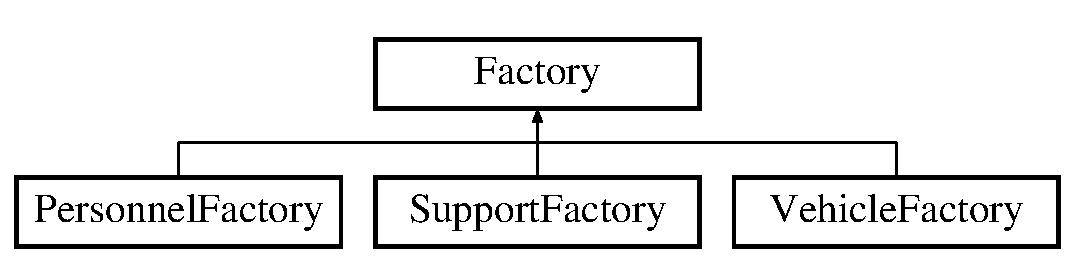
\includegraphics[height=2.000000cm]{classFactory}
\end{center}
\end{figure}
\doxysubsection*{Public Member Functions}
\begin{DoxyCompactItemize}
\item 
\mbox{\Hypertarget{classFactory_ac792bf88cfb7b6804b479529da5308cc}\label{classFactory_ac792bf88cfb7b6804b479529da5308cc}} 
\mbox{\hyperlink{classFactory_ac792bf88cfb7b6804b479529da5308cc}{Factory}} ()
\begin{DoxyCompactList}\small\item\em Instantiates the factory. \end{DoxyCompactList}\item 
void \mbox{\hyperlink{classFactory_a203d43ed769c39bac5dbe74e452a4222}{$\sim$\+Factory}} ()
\begin{DoxyCompactList}\small\item\em Destroys the factory object. \end{DoxyCompactList}\item 
\mbox{\Hypertarget{classFactory_a80da95da98b407948dc815f2bca6a283}\label{classFactory_a80da95da98b407948dc815f2bca6a283}} 
virtual \mbox{\hyperlink{classEntity}{Entity}} $\ast$ {\bfseries create\+Entity} (\mbox{\hyperlink{classAlliance}{Alliance}} $\ast$alliance)=0
\item 
\mbox{\hyperlink{classType}{Type}} $\ast$ \mbox{\hyperlink{classFactory_ac91051006ace7ec5bb6ecf0fe6d02d58}{get\+Type}} ()
\begin{DoxyCompactList}\small\item\em Returns factories type state. \end{DoxyCompactList}\item 
void \mbox{\hyperlink{classFactory_a7484d514b094114231dbeb3df70e9d0b}{set\+Type}} (\mbox{\hyperlink{classType}{Type}} $\ast$type)
\begin{DoxyCompactList}\small\item\em Sets the factories type state. \end{DoxyCompactList}\item 
\mbox{\hyperlink{classAddOn}{Add\+On}} $\ast$ \mbox{\hyperlink{classFactory_a46f89194541b0246a017f1eaf51ab654}{get\+Add\+Ons}} ()
\begin{DoxyCompactList}\small\item\em Returns factories add ons. \end{DoxyCompactList}\item 
void \mbox{\hyperlink{classFactory_a958217b0bc29ce69ace69ade5e701984}{set\+Add\+Ons}} (\mbox{\hyperlink{classAddOn}{Add\+On}} $\ast$add\+Ons)
\begin{DoxyCompactList}\small\item\em Sets the factories add ons. \end{DoxyCompactList}\item 
\mbox{\Hypertarget{classFactory_a00881ec5050751e4b747db5dfd266192}\label{classFactory_a00881ec5050751e4b747db5dfd266192}} 
virtual \mbox{\hyperlink{classFactory}{Factory}} $\ast$ {\bfseries clone} ()=0
\end{DoxyCompactItemize}


\doxysubsection{Detailed Description}
\mbox{\hyperlink{classFactory}{Factory}} class. 

Used to instantiate \mbox{\hyperlink{classEntity}{Entity}} objects. 

Definition at line 9 of file Factory.\+h.



\doxysubsection{Constructor \& Destructor Documentation}
\mbox{\Hypertarget{classFactory_a203d43ed769c39bac5dbe74e452a4222}\label{classFactory_a203d43ed769c39bac5dbe74e452a4222}} 
\index{Factory@{Factory}!````~Factory@{$\sim$Factory}}
\index{````~Factory@{$\sim$Factory}!Factory@{Factory}}
\doxysubsubsection{\texorpdfstring{$\sim$Factory()}{~Factory()}}
{\footnotesize\ttfamily void Factory\+::$\sim$\+Factory (\begin{DoxyParamCaption}{ }\end{DoxyParamCaption})}



Destroys the factory object. 

Postconditions\+:
\begin{DoxyItemize}
\item All dynamic memory should be deallocated from the factory object 
\end{DoxyItemize}

\doxysubsection{Member Function Documentation}
\mbox{\Hypertarget{classFactory_a46f89194541b0246a017f1eaf51ab654}\label{classFactory_a46f89194541b0246a017f1eaf51ab654}} 
\index{Factory@{Factory}!getAddOns@{getAddOns}}
\index{getAddOns@{getAddOns}!Factory@{Factory}}
\doxysubsubsection{\texorpdfstring{getAddOns()}{getAddOns()}}
{\footnotesize\ttfamily add\+On $\ast$ Factory\+::get\+Add\+Ons (\begin{DoxyParamCaption}{ }\end{DoxyParamCaption})}



Returns factories add ons. 

Postconditions\+:
\begin{DoxyItemize}
\item Returns the add ons of the factory
\end{DoxyItemize}

\begin{DoxyReturn}{Returns}
Add\+On$\ast$ The decorators for the factory object 
\end{DoxyReturn}


Definition at line 16 of file Factory.\+cpp.


\begin{DoxyCode}{0}
\DoxyCodeLine{16                           \{}
\DoxyCodeLine{17     \textcolor{keywordflow}{return} this-\/>addOns;}
\DoxyCodeLine{18 \}}

\end{DoxyCode}
\mbox{\Hypertarget{classFactory_ac91051006ace7ec5bb6ecf0fe6d02d58}\label{classFactory_ac91051006ace7ec5bb6ecf0fe6d02d58}} 
\index{Factory@{Factory}!getType@{getType}}
\index{getType@{getType}!Factory@{Factory}}
\doxysubsubsection{\texorpdfstring{getType()}{getType()}}
{\footnotesize\ttfamily \mbox{\hyperlink{classType}{Type}} $\ast$ Factory\+::get\+Type (\begin{DoxyParamCaption}{ }\end{DoxyParamCaption})}



Returns factories type state. 

Postconditions\+:
\begin{DoxyItemize}
\item Returns the type
\end{DoxyItemize}

\begin{DoxyReturn}{Returns}
Type$\ast$ The type state of the factory object 
\end{DoxyReturn}


Definition at line 8 of file Factory.\+cpp.


\begin{DoxyCode}{0}
\DoxyCodeLine{8                        \{}
\DoxyCodeLine{9     \textcolor{keywordflow}{return} this-\/>type;}
\DoxyCodeLine{10 \}}

\end{DoxyCode}
\mbox{\Hypertarget{classFactory_a958217b0bc29ce69ace69ade5e701984}\label{classFactory_a958217b0bc29ce69ace69ade5e701984}} 
\index{Factory@{Factory}!setAddOns@{setAddOns}}
\index{setAddOns@{setAddOns}!Factory@{Factory}}
\doxysubsubsection{\texorpdfstring{setAddOns()}{setAddOns()}}
{\footnotesize\ttfamily void Factory\+::set\+Add\+Ons (\begin{DoxyParamCaption}\item[{\mbox{\hyperlink{classAddOn}{Add\+On}} $\ast$}]{add\+Ons }\end{DoxyParamCaption})}



Sets the factories add ons. 

Preconditions\+:
\begin{DoxyItemize}
\item add\+Ons must be an Add\+On$\ast$
\end{DoxyItemize}

Postconditions\+:
\begin{DoxyItemize}
\item Sets the add ons of the factory object
\end{DoxyItemize}


\begin{DoxyParams}{Parameters}
{\em add\+Ons} & must be a Add\+On$\ast$ \\
\hline
\end{DoxyParams}
\begin{DoxyReturn}{Returns}
void 
\end{DoxyReturn}


Definition at line 20 of file Factory.\+cpp.


\begin{DoxyCode}{0}
\DoxyCodeLine{20                                      \{}
\DoxyCodeLine{21     this-\/>addOns = addOns;}
\DoxyCodeLine{22 \}}

\end{DoxyCode}
\mbox{\Hypertarget{classFactory_a7484d514b094114231dbeb3df70e9d0b}\label{classFactory_a7484d514b094114231dbeb3df70e9d0b}} 
\index{Factory@{Factory}!setType@{setType}}
\index{setType@{setType}!Factory@{Factory}}
\doxysubsubsection{\texorpdfstring{setType()}{setType()}}
{\footnotesize\ttfamily void Factory\+::set\+Type (\begin{DoxyParamCaption}\item[{\mbox{\hyperlink{classType}{Type}} $\ast$}]{type }\end{DoxyParamCaption})}



Sets the factories type state. 

Preconditions\+:
\begin{DoxyItemize}
\item type must be an Type$\ast$
\end{DoxyItemize}

Postconditions\+:
\begin{DoxyItemize}
\item Sets the type state of the factory object
\end{DoxyItemize}


\begin{DoxyParams}{Parameters}
{\em type} & must be a Type$\ast$ \\
\hline
\end{DoxyParams}
\begin{DoxyReturn}{Returns}
void 
\end{DoxyReturn}


Definition at line 12 of file Factory.\+cpp.


\begin{DoxyCode}{0}
\DoxyCodeLine{12                                 \{}
\DoxyCodeLine{13     this-\/>type = type;}
\DoxyCodeLine{14 \}}

\end{DoxyCode}


The documentation for this class was generated from the following files\+:\begin{DoxyCompactItemize}
\item 
Factory.\+h\item 
Factory.\+cpp\end{DoxyCompactItemize}

\hypertarget{classGeneral}{}\doxysection{General Class Reference}
\label{classGeneral}\index{General@{General}}
Inheritance diagram for General\+:\begin{figure}[H]
\begin{center}
\leavevmode
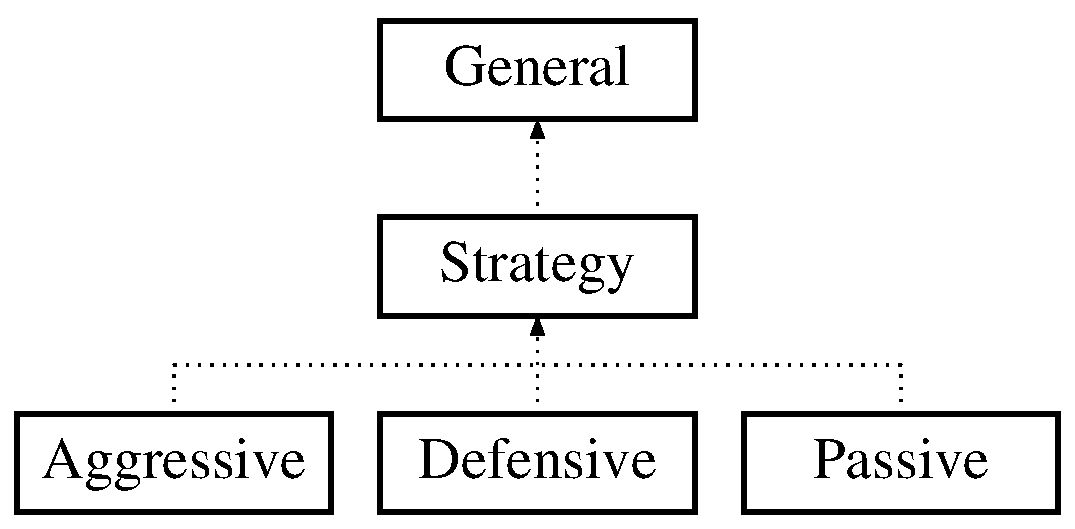
\includegraphics[height=3.000000cm]{classGeneral}
\end{center}
\end{figure}
\doxysubsection*{Public Member Functions}
\begin{DoxyCompactItemize}
\item 
\mbox{\Hypertarget{classGeneral_af4bee805ca5f7756c6d1f1c3fcde862a}\label{classGeneral_af4bee805ca5f7756c6d1f1c3fcde862a}} 
void {\bfseries evaluate\+Strategy} ()
\item 
\mbox{\Hypertarget{classGeneral_a449172bcf1b4bf8b9a47af6b4e435d7e}\label{classGeneral_a449172bcf1b4bf8b9a47af6b4e435d7e}} 
void {\bfseries initiate\+Strategy} ()
\item 
\mbox{\Hypertarget{classGeneral_a6c73103d464cf8f3ed95deea76d788d5}\label{classGeneral_a6c73103d464cf8f3ed95deea76d788d5}} 
\mbox{\hyperlink{classGeneral}{General}} $\ast$ {\bfseries clone} ()
\end{DoxyCompactItemize}


\doxysubsection{Detailed Description}


Definition at line 4 of file General.\+h.



The documentation for this class was generated from the following files\+:\begin{DoxyCompactItemize}
\item 
General.\+h\item 
General.\+cpp\end{DoxyCompactItemize}

\hypertarget{classKeyPoint}{}\doxysection{Key\+Point Class Reference}
\label{classKeyPoint}\index{KeyPoint@{KeyPoint}}


Keypoint class.  




{\ttfamily \#include $<$Key\+Point.\+h$>$}

Inheritance diagram for Key\+Point\+:\begin{figure}[H]
\begin{center}
\leavevmode
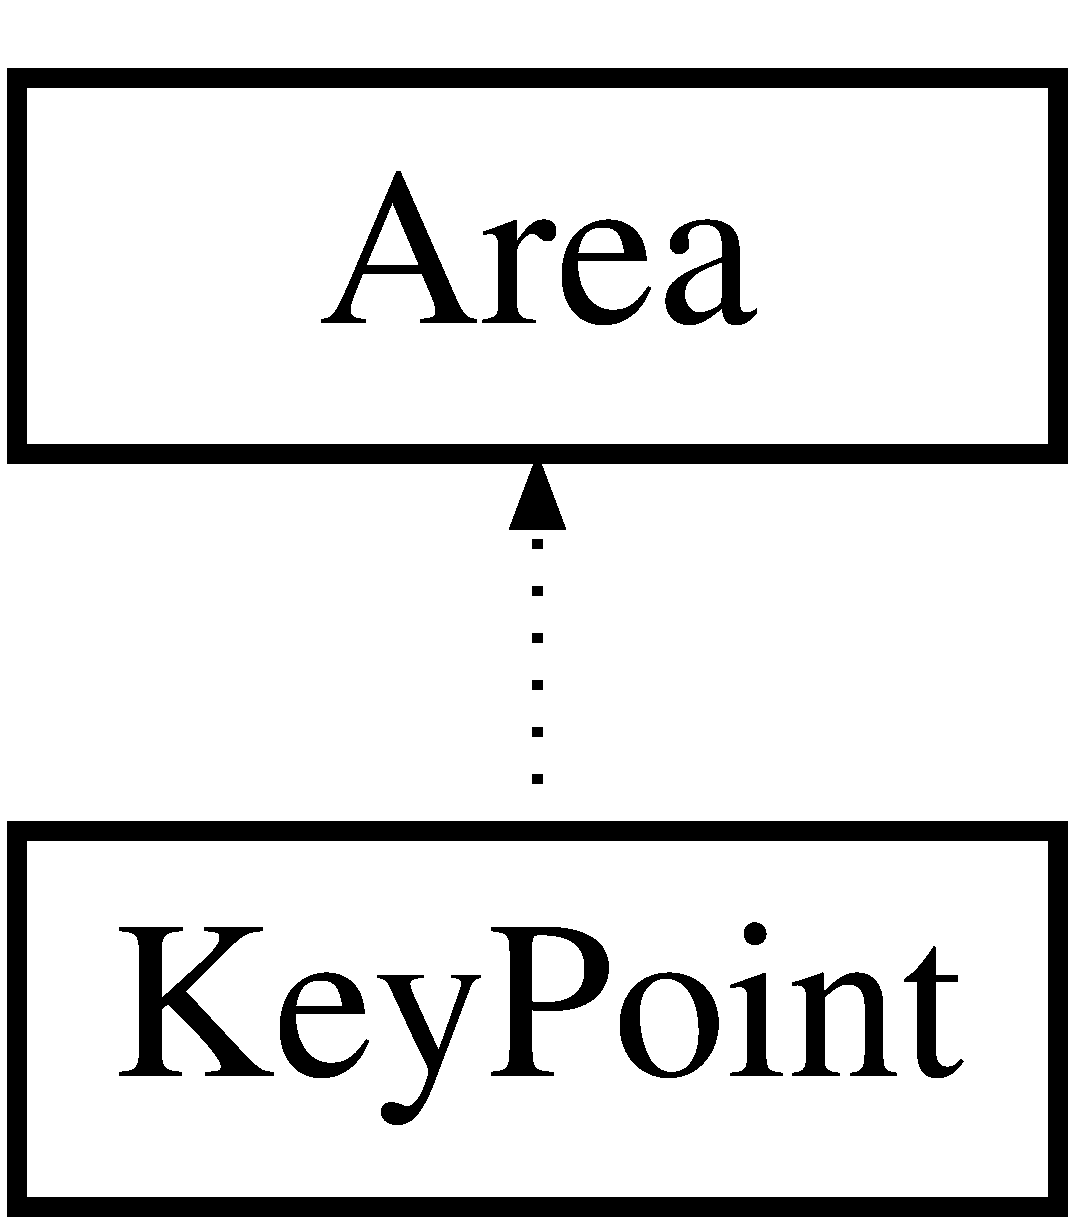
\includegraphics[height=2.000000cm]{classKeyPoint}
\end{center}
\end{figure}
\doxysubsection*{Public Member Functions}
\begin{DoxyCompactItemize}
\item 
\mbox{\hyperlink{classKeyPoint_a1e99a22c40a570c89b2d04cf67e98dd4}{Key\+Point}} (std\+::string area\+Name)
\begin{DoxyCompactList}\small\item\em Instantiates the key point. \end{DoxyCompactList}\item 
bool \mbox{\hyperlink{classKeyPoint_a1beb436d8efa973f3dc290a722727961}{is\+Key\+Point}} ()
\begin{DoxyCompactList}\small\item\em Returns area type. \end{DoxyCompactList}\item 
void \mbox{\hyperlink{classKeyPoint_a665afb6bb5b840d8101fb9d4d9e96cd7}{simulate\+Battle}} (\mbox{\hyperlink{classAlliance}{Alliance}} $\ast$alliance)
\begin{DoxyCompactList}\small\item\em Simulate Battle with troops from the alliance passed in. \end{DoxyCompactList}\item 
void \mbox{\hyperlink{classKeyPoint_aa43cf43a4d0272f8511f3a79d2dc143b}{clear\+Battlefield}} ()
\begin{DoxyCompactList}\small\item\em Clears the battlefield of all deceased troops. \end{DoxyCompactList}\item 
void \mbox{\hyperlink{classKeyPoint_a4d98646584dffb8e4d59c600e693cfe6}{move\+Entities\+Into}} (\mbox{\hyperlink{classAlliance}{Alliance}} $\ast$alliance, int num\+Troops)
\begin{DoxyCompactList}\small\item\em Moves a specific alliances troops into this keypoint. \end{DoxyCompactList}\item 
void \mbox{\hyperlink{classKeyPoint_aa5bb6fa677e0b560adfb95e0ff30aa8a}{move\+Entities\+Out\+Of}} (\mbox{\hyperlink{classAlliance}{Alliance}} $\ast$alliance, int num\+Troops)
\begin{DoxyCompactList}\small\item\em Moves a specific alliances troops out of the keypoint. \end{DoxyCompactList}\item 
void \mbox{\hyperlink{classKeyPoint_aad6d7102c8e3d11fe5f29b163f50dbc3}{add\+Entity}} (\mbox{\hyperlink{classEntity}{Entity}} $\ast$entity)
\begin{DoxyCompactList}\small\item\em Adds an enitity to the key point object. \end{DoxyCompactList}\item 
void \mbox{\hyperlink{classKeyPoint_adef7a6b2e761e720e9b08890106ae257}{add\+General}} (\mbox{\hyperlink{classGeneral}{General}} $\ast$general)
\item 
void \mbox{\hyperlink{classKeyPoint_abe2ba3c8d36eb45711f396ff295fa32e}{remove\+General}} (\mbox{\hyperlink{classGeneral}{General}} $\ast$general)
\item 
\mbox{\hyperlink{classArea}{Area}} $\ast$ \mbox{\hyperlink{classKeyPoint_adc4679ca31d34b0ae3fedded47e27938}{clone}} ()
\begin{DoxyCompactList}\small\item\em Instantiates and returns a clone of the current Keypoint. \end{DoxyCompactList}\item 
void \mbox{\hyperlink{classKeyPoint_a1906ddf2b2b5d1bf81e82605b3eb63a0}{change\+Weather}} ()
\begin{DoxyCompactList}\small\item\em Switches the \mbox{\hyperlink{classWeather}{Weather}} object to the next state. \end{DoxyCompactList}\item 
void \mbox{\hyperlink{classKeyPoint_a5c4b9314440a00fca7ab4d82ea4693a5}{set\+Weather}} (\mbox{\hyperlink{classWeather}{Weather}} $\ast$weather)
\begin{DoxyCompactList}\small\item\em Set the \mbox{\hyperlink{classWeather}{Weather}} object. \end{DoxyCompactList}\item 
std\+::string \mbox{\hyperlink{classKeyPoint_a8e5315f1f4dd2427206e13709eed48e2}{get\+Weather}} () const
\begin{DoxyCompactList}\small\item\em The weather at the current state is returned. \end{DoxyCompactList}\end{DoxyCompactItemize}


\doxysubsection{Detailed Description}
Keypoint class. 

Used to emulate strategic positions. 

Definition at line \mbox{\hyperlink{KeyPoint_8h_source_l00017}{17}} of file \mbox{\hyperlink{KeyPoint_8h_source}{Key\+Point.\+h}}.



\doxysubsection{Constructor \& Destructor Documentation}
\mbox{\Hypertarget{classKeyPoint_a1e99a22c40a570c89b2d04cf67e98dd4}\label{classKeyPoint_a1e99a22c40a570c89b2d04cf67e98dd4}} 
\index{KeyPoint@{KeyPoint}!KeyPoint@{KeyPoint}}
\index{KeyPoint@{KeyPoint}!KeyPoint@{KeyPoint}}
\doxysubsubsection{\texorpdfstring{KeyPoint()}{KeyPoint()}}
{\footnotesize\ttfamily Key\+Point\+::\+Key\+Point (\begin{DoxyParamCaption}\item[{std\+::string}]{area\+Name }\end{DoxyParamCaption})}



Instantiates the key point. 



Definition at line \mbox{\hyperlink{KeyPoint_8cpp_source_l00008}{8}} of file \mbox{\hyperlink{KeyPoint_8cpp_source}{Key\+Point.\+cpp}}.


\begin{DoxyCode}{0}
\DoxyCodeLine{00008 : \mbox{\hyperlink{classArea}{Area}}(areaName) \{\}}

\end{DoxyCode}
\mbox{\Hypertarget{classKeyPoint_a6bf5e6613c329a8f2afeb8c66aa116bd}\label{classKeyPoint_a6bf5e6613c329a8f2afeb8c66aa116bd}} 
\index{KeyPoint@{KeyPoint}!````~KeyPoint@{$\sim$KeyPoint}}
\index{````~KeyPoint@{$\sim$KeyPoint}!KeyPoint@{KeyPoint}}
\doxysubsubsection{\texorpdfstring{$\sim$KeyPoint()}{~KeyPoint()}}
{\footnotesize\ttfamily Key\+Point\+::$\sim$\+Key\+Point (\begin{DoxyParamCaption}{ }\end{DoxyParamCaption})}



Definition at line \mbox{\hyperlink{KeyPoint_8cpp_source_l00010}{10}} of file \mbox{\hyperlink{KeyPoint_8cpp_source}{Key\+Point.\+cpp}}.


\begin{DoxyCode}{0}
\DoxyCodeLine{00010                     \{}
\DoxyCodeLine{00011     \textcolor{keywordflow}{for} (\textcolor{keywordtype}{int} i = 0; i < entities.size(); i++)}
\DoxyCodeLine{00012         \textcolor{keyword}{delete} entities[i];}
\DoxyCodeLine{00013 }
\DoxyCodeLine{00014     \textcolor{keywordflow}{for} (\textcolor{keywordtype}{int} i = 0; i < generals.size(); i++)}
\DoxyCodeLine{00015         \textcolor{keyword}{delete} generals[i];}
\DoxyCodeLine{00016 }
\DoxyCodeLine{00017     \textcolor{keyword}{delete} weather;}
\DoxyCodeLine{00018 \}}

\end{DoxyCode}


\doxysubsection{Member Function Documentation}
\mbox{\Hypertarget{classKeyPoint_aad6d7102c8e3d11fe5f29b163f50dbc3}\label{classKeyPoint_aad6d7102c8e3d11fe5f29b163f50dbc3}} 
\index{KeyPoint@{KeyPoint}!addEntity@{addEntity}}
\index{addEntity@{addEntity}!KeyPoint@{KeyPoint}}
\doxysubsubsection{\texorpdfstring{addEntity()}{addEntity()}}
{\footnotesize\ttfamily void Key\+Point\+::add\+Entity (\begin{DoxyParamCaption}\item[{\mbox{\hyperlink{classEntity}{Entity}} $\ast$}]{entity }\end{DoxyParamCaption})}



Adds an enitity to the key point object. 

Preconditions\+:
\begin{DoxyItemize}
\item entity must be an Entity$\ast$
\end{DoxyItemize}

Postconditions\+:
\begin{DoxyItemize}
\item Add entity to key point
\end{DoxyItemize}


\begin{DoxyParams}{Parameters}
{\em entity} & must be an Entity$\ast$ \\
\hline
\end{DoxyParams}
\begin{DoxyReturn}{Returns}
void 
\end{DoxyReturn}


Definition at line \mbox{\hyperlink{KeyPoint_8cpp_source_l00070}{70}} of file \mbox{\hyperlink{KeyPoint_8cpp_source}{Key\+Point.\+cpp}}.


\begin{DoxyCode}{0}
\DoxyCodeLine{00070                                        \{}
\DoxyCodeLine{00071     entities.push\_back(entity);}
\DoxyCodeLine{00072 \}}

\end{DoxyCode}
\mbox{\Hypertarget{classKeyPoint_adef7a6b2e761e720e9b08890106ae257}\label{classKeyPoint_adef7a6b2e761e720e9b08890106ae257}} 
\index{KeyPoint@{KeyPoint}!addGeneral@{addGeneral}}
\index{addGeneral@{addGeneral}!KeyPoint@{KeyPoint}}
\doxysubsubsection{\texorpdfstring{addGeneral()}{addGeneral()}}
{\footnotesize\ttfamily void Key\+Point\+::add\+General (\begin{DoxyParamCaption}\item[{\mbox{\hyperlink{classGeneral}{General}} $\ast$}]{general }\end{DoxyParamCaption})}



Definition at line \mbox{\hyperlink{KeyPoint_8cpp_source_l00074}{74}} of file \mbox{\hyperlink{KeyPoint_8cpp_source}{Key\+Point.\+cpp}}.


\begin{DoxyCode}{0}
\DoxyCodeLine{00074                                           \{}
\DoxyCodeLine{00075     generals.push\_back(general);}
\DoxyCodeLine{00076 \}}

\end{DoxyCode}
\mbox{\Hypertarget{classKeyPoint_a1906ddf2b2b5d1bf81e82605b3eb63a0}\label{classKeyPoint_a1906ddf2b2b5d1bf81e82605b3eb63a0}} 
\index{KeyPoint@{KeyPoint}!changeWeather@{changeWeather}}
\index{changeWeather@{changeWeather}!KeyPoint@{KeyPoint}}
\doxysubsubsection{\texorpdfstring{changeWeather()}{changeWeather()}}
{\footnotesize\ttfamily void Key\+Point\+::change\+Weather (\begin{DoxyParamCaption}{ }\end{DoxyParamCaption})}



Switches the \mbox{\hyperlink{classWeather}{Weather}} object to the next state. 



Definition at line \mbox{\hyperlink{KeyPoint_8cpp_source_l00098}{98}} of file \mbox{\hyperlink{KeyPoint_8cpp_source}{Key\+Point.\+cpp}}.


\begin{DoxyCode}{0}
\DoxyCodeLine{00098                              \{}
\DoxyCodeLine{00099 }
\DoxyCodeLine{00100     srand(time(0));}
\DoxyCodeLine{00101 }
\DoxyCodeLine{00102     \textcolor{keywordtype}{int} randomNum = 1 + (rand() \% 10);}
\DoxyCodeLine{00103     std::string currWeather = this-\/>weather-\/>getWeather();}
\DoxyCodeLine{00104 }
\DoxyCodeLine{00105     \textcolor{keywordflow}{if} (currWeather == \textcolor{stringliteral}{"{}Sunny"{}} \&\& randomNum > 6) \textcolor{comment}{// 60\% chance of not changing weather from Sunny and staying}}
\DoxyCodeLine{00106         this-\/>weather-\/>handleChange(\textcolor{keyword}{this});}
\DoxyCodeLine{00107     \textcolor{keywordflow}{else} \textcolor{keywordflow}{if} (currWeather == \textcolor{stringliteral}{"{}Cloudy"{}} \&\& randomNum > 3) \textcolor{comment}{// 30\% chance of not changing weather from Cloudy and staying}}
\DoxyCodeLine{00108         this-\/>weather-\/>handleChange(\textcolor{keyword}{this});}
\DoxyCodeLine{00109     \textcolor{keywordflow}{else} \textcolor{keywordflow}{if} (currWeather == \textcolor{stringliteral}{"{}Rainy"{}} \&\& randomNum > 1) \textcolor{comment}{// 10\% chance of not changing weather from Rainy and staying}}
\DoxyCodeLine{00110         this-\/>weather-\/>handleChange(\textcolor{keyword}{this});}
\DoxyCodeLine{00111     }
\DoxyCodeLine{00112 }
\DoxyCodeLine{00113 \}}

\end{DoxyCode}
\mbox{\Hypertarget{classKeyPoint_aa43cf43a4d0272f8511f3a79d2dc143b}\label{classKeyPoint_aa43cf43a4d0272f8511f3a79d2dc143b}} 
\index{KeyPoint@{KeyPoint}!clearBattlefield@{clearBattlefield}}
\index{clearBattlefield@{clearBattlefield}!KeyPoint@{KeyPoint}}
\doxysubsubsection{\texorpdfstring{clearBattlefield()}{clearBattlefield()}}
{\footnotesize\ttfamily void Key\+Point\+::clear\+Battlefield (\begin{DoxyParamCaption}{ }\end{DoxyParamCaption})}



Clears the battlefield of all deceased troops. 

Postconditions\+:
\begin{DoxyItemize}
\item Notify command centers of each troop who is killed
\end{DoxyItemize}

\begin{DoxyReturn}{Returns}
void 
\end{DoxyReturn}


Definition at line \mbox{\hyperlink{KeyPoint_8cpp_source_l00038}{38}} of file \mbox{\hyperlink{KeyPoint_8cpp_source}{Key\+Point.\+cpp}}.


\begin{DoxyCode}{0}
\DoxyCodeLine{00038                                 \{}
\DoxyCodeLine{00039     \textcolor{keywordflow}{for} (vector<Entity*>::iterator it = entities.begin();  it != entities.end(); ++it) \{}
\DoxyCodeLine{00040         \textcolor{keywordflow}{if} ((*it)-\/>getHealth() <= 0) \{}
\DoxyCodeLine{00041             \textcolor{keywordflow}{for} (\textcolor{keywordtype}{int} i = 0; i < generals.size(); i++) \{}
\DoxyCodeLine{00042                 \textcolor{keywordflow}{if} (generals[i]-\/>getAlliance() == (*it)-\/>getAlliance()) \{}
\DoxyCodeLine{00043                     generals[i]-\/>initiateStrategy(\textcolor{keyword}{this});}
\DoxyCodeLine{00044                     \textcolor{keyword}{delete} *it;}
\DoxyCodeLine{00045                     entities.erase(it);}
\DoxyCodeLine{00046                 \}}
\DoxyCodeLine{00047             \}}
\DoxyCodeLine{00048         \}}
\DoxyCodeLine{00049     \}}
\DoxyCodeLine{00050 \}}

\end{DoxyCode}
\mbox{\Hypertarget{classKeyPoint_adc4679ca31d34b0ae3fedded47e27938}\label{classKeyPoint_adc4679ca31d34b0ae3fedded47e27938}} 
\index{KeyPoint@{KeyPoint}!clone@{clone}}
\index{clone@{clone}!KeyPoint@{KeyPoint}}
\doxysubsubsection{\texorpdfstring{clone()}{clone()}}
{\footnotesize\ttfamily \mbox{\hyperlink{classArea}{Area}} $\ast$ Key\+Point\+::clone (\begin{DoxyParamCaption}{ }\end{DoxyParamCaption})\hspace{0.3cm}{\ttfamily [virtual]}}



Instantiates and returns a clone of the current Keypoint. 

Postconditions\+:
\begin{DoxyItemize}
\item Returns the clone of the current Keypoint
\end{DoxyItemize}

\begin{DoxyReturn}{Returns}
Area$\ast$ The Keypoint clone 
\end{DoxyReturn}


Implements \mbox{\hyperlink{classArea}{Area}}.



Definition at line \mbox{\hyperlink{KeyPoint_8cpp_source_l00088}{88}} of file \mbox{\hyperlink{KeyPoint_8cpp_source}{Key\+Point.\+cpp}}.


\begin{DoxyCode}{0}
\DoxyCodeLine{00088                       \{}
\DoxyCodeLine{00089     \textcolor{comment}{// TODO -\/ implement KeyPoint::clone}}
\DoxyCodeLine{00090     \textcolor{keywordflow}{throw} \textcolor{stringliteral}{"{}Not yet implemented"{}};}
\DoxyCodeLine{00091 \}}

\end{DoxyCode}
\mbox{\Hypertarget{classKeyPoint_a8e5315f1f4dd2427206e13709eed48e2}\label{classKeyPoint_a8e5315f1f4dd2427206e13709eed48e2}} 
\index{KeyPoint@{KeyPoint}!getWeather@{getWeather}}
\index{getWeather@{getWeather}!KeyPoint@{KeyPoint}}
\doxysubsubsection{\texorpdfstring{getWeather()}{getWeather()}}
{\footnotesize\ttfamily std\+::string Key\+Point\+::get\+Weather (\begin{DoxyParamCaption}{ }\end{DoxyParamCaption}) const}



The weather at the current state is returned. 

\begin{DoxyReturn}{Returns}
string The weather state 
\end{DoxyReturn}


Definition at line \mbox{\hyperlink{KeyPoint_8cpp_source_l00115}{115}} of file \mbox{\hyperlink{KeyPoint_8cpp_source}{Key\+Point.\+cpp}}.


\begin{DoxyCode}{0}
\DoxyCodeLine{00115                                      \{}
\DoxyCodeLine{00116     \textcolor{keywordflow}{return} this-\/>weather-\/>getWeather();}
\DoxyCodeLine{00117 \}}

\end{DoxyCode}
\mbox{\Hypertarget{classKeyPoint_a1beb436d8efa973f3dc290a722727961}\label{classKeyPoint_a1beb436d8efa973f3dc290a722727961}} 
\index{KeyPoint@{KeyPoint}!isKeyPoint@{isKeyPoint}}
\index{isKeyPoint@{isKeyPoint}!KeyPoint@{KeyPoint}}
\doxysubsubsection{\texorpdfstring{isKeyPoint()}{isKeyPoint()}}
{\footnotesize\ttfamily bool Key\+Point\+::is\+Key\+Point (\begin{DoxyParamCaption}{ }\end{DoxyParamCaption})\hspace{0.3cm}{\ttfamily [virtual]}}



Returns area type. 

Postconditions\+:
\begin{DoxyItemize}
\item Returns true
\end{DoxyItemize}

\begin{DoxyReturn}{Returns}
bool The area type 
\end{DoxyReturn}


Implements \mbox{\hyperlink{classArea}{Area}}.



Definition at line \mbox{\hyperlink{KeyPoint_8cpp_source_l00020}{20}} of file \mbox{\hyperlink{KeyPoint_8cpp_source}{Key\+Point.\+cpp}}.


\begin{DoxyCode}{0}
\DoxyCodeLine{00020                           \{}
\DoxyCodeLine{00021     \textcolor{keywordflow}{return} \textcolor{keyword}{true};}
\DoxyCodeLine{00022 \}}

\end{DoxyCode}
\mbox{\Hypertarget{classKeyPoint_a4d98646584dffb8e4d59c600e693cfe6}\label{classKeyPoint_a4d98646584dffb8e4d59c600e693cfe6}} 
\index{KeyPoint@{KeyPoint}!moveEntitiesInto@{moveEntitiesInto}}
\index{moveEntitiesInto@{moveEntitiesInto}!KeyPoint@{KeyPoint}}
\doxysubsubsection{\texorpdfstring{moveEntitiesInto()}{moveEntitiesInto()}}
{\footnotesize\ttfamily void Key\+Point\+::move\+Entities\+Into (\begin{DoxyParamCaption}\item[{\mbox{\hyperlink{classAlliance}{Alliance}} $\ast$}]{alliance,  }\item[{int}]{num\+Troops }\end{DoxyParamCaption})}



Moves a specific alliances troops into this keypoint. 

Preconditions\+:
\begin{DoxyItemize}
\item alliance must be an Alliance$\ast$
\item num\+Troops must be an int
\end{DoxyItemize}

Postconditions\+:
\begin{DoxyItemize}
\item Move troops to into this keypoint
\end{DoxyItemize}


\begin{DoxyParams}{Parameters}
{\em alliance} & must be an Alliance$\ast$ \\
\hline
{\em num\+Troops} & must be an int \\
\hline
\end{DoxyParams}
\begin{DoxyReturn}{Returns}
void 
\end{DoxyReturn}


Definition at line \mbox{\hyperlink{KeyPoint_8cpp_source_l00052}{52}} of file \mbox{\hyperlink{KeyPoint_8cpp_source}{Key\+Point.\+cpp}}.


\begin{DoxyCode}{0}
\DoxyCodeLine{00052                                                                  \{}
\DoxyCodeLine{00053     vector<Entity*> troops = alliance-\/>\mbox{\hyperlink{classAlliance_a8c93c88d5624a3445814b86496ad68d7}{getReserveEntities}}(numTroops);}
\DoxyCodeLine{00054     \textcolor{keywordflow}{for} (\textcolor{keywordtype}{int} i = 0; i < troops.size(); i++)}
\DoxyCodeLine{00055         entities.push\_back(troops[i]);}
\DoxyCodeLine{00056 \}}

\end{DoxyCode}
\mbox{\Hypertarget{classKeyPoint_aa5bb6fa677e0b560adfb95e0ff30aa8a}\label{classKeyPoint_aa5bb6fa677e0b560adfb95e0ff30aa8a}} 
\index{KeyPoint@{KeyPoint}!moveEntitiesOutOf@{moveEntitiesOutOf}}
\index{moveEntitiesOutOf@{moveEntitiesOutOf}!KeyPoint@{KeyPoint}}
\doxysubsubsection{\texorpdfstring{moveEntitiesOutOf()}{moveEntitiesOutOf()}}
{\footnotesize\ttfamily void Key\+Point\+::move\+Entities\+Out\+Of (\begin{DoxyParamCaption}\item[{\mbox{\hyperlink{classAlliance}{Alliance}} $\ast$}]{alliance,  }\item[{int}]{num\+Troops }\end{DoxyParamCaption})}



Moves a specific alliances troops out of the keypoint. 

Preconditions\+:
\begin{DoxyItemize}
\item alliance must be an Alliance$\ast$
\item num\+Troops must be an int
\end{DoxyItemize}

Postconditions\+:
\begin{DoxyItemize}
\item Move troops to reserve
\end{DoxyItemize}


\begin{DoxyParams}{Parameters}
{\em alliance} & must be an Alliance$\ast$ \\
\hline
{\em num\+Troops} & must be an int \\
\hline
\end{DoxyParams}
\begin{DoxyReturn}{Returns}
void 
\end{DoxyReturn}


Definition at line \mbox{\hyperlink{KeyPoint_8cpp_source_l00058}{58}} of file \mbox{\hyperlink{KeyPoint_8cpp_source}{Key\+Point.\+cpp}}.


\begin{DoxyCode}{0}
\DoxyCodeLine{00058                                                                   \{}
\DoxyCodeLine{00059     vector<Entity*>::iterator it = entities.begin();}
\DoxyCodeLine{00060     \textcolor{keywordflow}{for} (\textcolor{keywordtype}{int} i = 0; i < numTroops \&\& it != entities.end(); i++) \{}
\DoxyCodeLine{00061         \textcolor{keywordflow}{for} (; it != entities.end(); ++it) \{}
\DoxyCodeLine{00062             \textcolor{keywordflow}{if} ((*it)-\/>getAlliance() == alliance) \{}
\DoxyCodeLine{00063                 alliance-\/>\mbox{\hyperlink{classAlliance_a37c4045fb37caf729d1f8f266f5f1bf0}{addReserveEntity}}(*it);}
\DoxyCodeLine{00064                 entities.erase(it);}
\DoxyCodeLine{00065             \}}
\DoxyCodeLine{00066         \}}
\DoxyCodeLine{00067     \}}
\DoxyCodeLine{00068 \}}

\end{DoxyCode}
\mbox{\Hypertarget{classKeyPoint_abe2ba3c8d36eb45711f396ff295fa32e}\label{classKeyPoint_abe2ba3c8d36eb45711f396ff295fa32e}} 
\index{KeyPoint@{KeyPoint}!removeGeneral@{removeGeneral}}
\index{removeGeneral@{removeGeneral}!KeyPoint@{KeyPoint}}
\doxysubsubsection{\texorpdfstring{removeGeneral()}{removeGeneral()}}
{\footnotesize\ttfamily void Key\+Point\+::remove\+General (\begin{DoxyParamCaption}\item[{\mbox{\hyperlink{classGeneral}{General}} $\ast$}]{general }\end{DoxyParamCaption})}



Definition at line \mbox{\hyperlink{KeyPoint_8cpp_source_l00078}{78}} of file \mbox{\hyperlink{KeyPoint_8cpp_source}{Key\+Point.\+cpp}}.


\begin{DoxyCode}{0}
\DoxyCodeLine{00078                                              \{}
\DoxyCodeLine{00079     \textcolor{keywordflow}{for} (vector<General*>::iterator it = generals.begin();  it != generals.end(); ++it) \{}
\DoxyCodeLine{00080         \textcolor{keywordflow}{if} (*it == general) \{}
\DoxyCodeLine{00081             \textcolor{keyword}{delete} *it;}
\DoxyCodeLine{00082             generals.erase(it);}
\DoxyCodeLine{00083             \textcolor{keywordflow}{return};}
\DoxyCodeLine{00084         \}}
\DoxyCodeLine{00085     \}}
\DoxyCodeLine{00086 \}}

\end{DoxyCode}
\mbox{\Hypertarget{classKeyPoint_a5c4b9314440a00fca7ab4d82ea4693a5}\label{classKeyPoint_a5c4b9314440a00fca7ab4d82ea4693a5}} 
\index{KeyPoint@{KeyPoint}!setWeather@{setWeather}}
\index{setWeather@{setWeather}!KeyPoint@{KeyPoint}}
\doxysubsubsection{\texorpdfstring{setWeather()}{setWeather()}}
{\footnotesize\ttfamily void Key\+Point\+::set\+Weather (\begin{DoxyParamCaption}\item[{\mbox{\hyperlink{classWeather}{Weather}} $\ast$}]{weather }\end{DoxyParamCaption})}



Set the \mbox{\hyperlink{classWeather}{Weather}} object. 

Preconditions\+:
\begin{DoxyItemize}
\item weather must be a Weather$\ast$
\end{DoxyItemize}

Postconditions\+:
\begin{DoxyItemize}
\item must set the key\+Points weather state
\end{DoxyItemize}


\begin{DoxyParams}{Parameters}
{\em weather} & must be a Weather$\ast$ \\
\hline
\end{DoxyParams}
\begin{DoxyReturn}{Returns}
void 
\end{DoxyReturn}


Definition at line \mbox{\hyperlink{KeyPoint_8cpp_source_l00093}{93}} of file \mbox{\hyperlink{KeyPoint_8cpp_source}{Key\+Point.\+cpp}}.


\begin{DoxyCode}{0}
\DoxyCodeLine{00093                                           \{}
\DoxyCodeLine{00094     \textcolor{keyword}{delete} this-\/>weather;}
\DoxyCodeLine{00095     this-\/>weather = weather;}
\DoxyCodeLine{00096 \}}

\end{DoxyCode}
\mbox{\Hypertarget{classKeyPoint_a665afb6bb5b840d8101fb9d4d9e96cd7}\label{classKeyPoint_a665afb6bb5b840d8101fb9d4d9e96cd7}} 
\index{KeyPoint@{KeyPoint}!simulateBattle@{simulateBattle}}
\index{simulateBattle@{simulateBattle}!KeyPoint@{KeyPoint}}
\doxysubsubsection{\texorpdfstring{simulateBattle()}{simulateBattle()}}
{\footnotesize\ttfamily void Key\+Point\+::simulate\+Battle (\begin{DoxyParamCaption}\item[{\mbox{\hyperlink{classAlliance}{Alliance}} $\ast$}]{alliance }\end{DoxyParamCaption})\hspace{0.3cm}{\ttfamily [virtual]}}



Simulate Battle with troops from the alliance passed in. 

Preconditions\+:
\begin{DoxyItemize}
\item alliance must be an Alliance$\ast$
\end{DoxyItemize}

Postconditions\+:
\begin{DoxyItemize}
\item Perform attacks on other alliance troops
\end{DoxyItemize}


\begin{DoxyParams}{Parameters}
{\em alliance} & must be an Alliance$\ast$ \\
\hline
\end{DoxyParams}
\begin{DoxyReturn}{Returns}
void 
\end{DoxyReturn}


Implements \mbox{\hyperlink{classArea}{Area}}.



Definition at line \mbox{\hyperlink{KeyPoint_8cpp_source_l00024}{24}} of file \mbox{\hyperlink{KeyPoint_8cpp_source}{Key\+Point.\+cpp}}.


\begin{DoxyCode}{0}
\DoxyCodeLine{00024                                                 \{}
\DoxyCodeLine{00025     \textcolor{keywordflow}{for} (\textcolor{keywordtype}{int} i = 0; i < entities.size(); i++) \{}
\DoxyCodeLine{00026         \textcolor{keywordflow}{if} (entities[i]-\/>getAlliance() == alliance) \{}
\DoxyCodeLine{00027             \textcolor{keywordtype}{int} random;}
\DoxyCodeLine{00028             \textcolor{keywordflow}{do} \{}
\DoxyCodeLine{00029                 random = rand() \% entities.size();}
\DoxyCodeLine{00030             \} \textcolor{keywordflow}{while} (entities[random]-\/>getAlliance() == alliance);}
\DoxyCodeLine{00031 }
\DoxyCodeLine{00032             \textcolor{keywordflow}{if} (rand() \% (\textcolor{keywordtype}{int})(weather-\/>\mbox{\hyperlink{classWeather_a608d4dbf5437b576d131fe92bf8b81d7}{getMultiplier}}() * 100) <= (\textcolor{keywordtype}{int})(weather-\/>\mbox{\hyperlink{classWeather_a608d4dbf5437b576d131fe92bf8b81d7}{getMultiplier}}() * 100))}
\DoxyCodeLine{00033                 entities[i]-\/>dealDamage(entities[random]);}
\DoxyCodeLine{00034         \}}
\DoxyCodeLine{00035     \}}
\DoxyCodeLine{00036 \}}

\end{DoxyCode}


The documentation for this class was generated from the following files\+:\begin{DoxyCompactItemize}
\item 
Key\+Point.\+h\item 
Key\+Point.\+cpp\end{DoxyCompactItemize}

\hypertarget{classNegotiator}{}\doxysection{Negotiator Class Reference}
\label{classNegotiator}\index{Negotiator@{Negotiator}}
\doxysubsection*{Public Member Functions}
\begin{DoxyCompactItemize}
\item 
\mbox{\hyperlink{classNegotiator_aa667cc5e0bca1109e2eae6d84e8ba3d9}{Negotiator}} ()
\begin{DoxyCompactList}\small\item\em Instantiates the \mbox{\hyperlink{classNegotiator}{Negotiator}}. \end{DoxyCompactList}\item 
\mbox{\hyperlink{classNegotiator_add27a41f80fee92e8471b8ee9d9905f6}{$\sim$\+Negotiator}} ()
\begin{DoxyCompactList}\small\item\em Destructor for the \mbox{\hyperlink{classNegotiator}{Negotiator}} object. \end{DoxyCompactList}\item 
bool \mbox{\hyperlink{classNegotiator_aa95e7f447a76c6d5ef84b92731ccb00d}{send\+Peace}} (\mbox{\hyperlink{classAlliance}{Alliance}} $\ast$offer\+Alliance)
\begin{DoxyCompactList}\small\item\em Tries to offer peace to all the alliances in vector. \end{DoxyCompactList}\item 
void \mbox{\hyperlink{classNegotiator_ac6ec48dbce55bf196c299342695054ef}{remove\+Alliance}} (\mbox{\hyperlink{classAlliance}{Alliance}} $\ast$old\+Alliance)
\begin{DoxyCompactList}\small\item\em Removes an alliance from the alliance vector. \end{DoxyCompactList}\item 
void \mbox{\hyperlink{classNegotiator_acff1b9b66c8c7761d687b47a1a75883a}{add\+Alliance}} (\mbox{\hyperlink{classAlliance}{Alliance}} $\ast$new\+Alliance)
\begin{DoxyCompactList}\small\item\em Adds an alliance to the alliance vector. \end{DoxyCompactList}\item 
int \mbox{\hyperlink{classNegotiator_a20af02012820a0296ac14f75e0b87282}{get\+Num\+Alliances}} ()
\item 
\mbox{\hyperlink{classNegotiator}{Negotiator}} $\ast$ \mbox{\hyperlink{classNegotiator_adafefed500d3f36649696b3d2fc92be7}{clone}} ()
\begin{DoxyCompactList}\small\item\em Instantiates and returns a clone of the current \mbox{\hyperlink{classNegotiator}{Negotiator}}. \end{DoxyCompactList}\end{DoxyCompactItemize}


\doxysubsection{Detailed Description}


Definition at line \mbox{\hyperlink{Negotiator_8h_source_l00006}{6}} of file \mbox{\hyperlink{Negotiator_8h_source}{Negotiator.\+h}}.



\doxysubsection{Constructor \& Destructor Documentation}
\mbox{\Hypertarget{classNegotiator_aa667cc5e0bca1109e2eae6d84e8ba3d9}\label{classNegotiator_aa667cc5e0bca1109e2eae6d84e8ba3d9}} 
\index{Negotiator@{Negotiator}!Negotiator@{Negotiator}}
\index{Negotiator@{Negotiator}!Negotiator@{Negotiator}}
\doxysubsubsection{\texorpdfstring{Negotiator()}{Negotiator()}}
{\footnotesize\ttfamily Negotiator\+::\+Negotiator (\begin{DoxyParamCaption}{ }\end{DoxyParamCaption})}



Instantiates the \mbox{\hyperlink{classNegotiator}{Negotiator}}. 



Definition at line \mbox{\hyperlink{Negotiator_8cpp_source_l00004}{4}} of file \mbox{\hyperlink{Negotiator_8cpp_source}{Negotiator.\+cpp}}.


\begin{DoxyCode}{0}
\DoxyCodeLine{00004 \{\}}

\end{DoxyCode}
\mbox{\Hypertarget{classNegotiator_add27a41f80fee92e8471b8ee9d9905f6}\label{classNegotiator_add27a41f80fee92e8471b8ee9d9905f6}} 
\index{Negotiator@{Negotiator}!````~Negotiator@{$\sim$Negotiator}}
\index{````~Negotiator@{$\sim$Negotiator}!Negotiator@{Negotiator}}
\doxysubsubsection{\texorpdfstring{$\sim$Negotiator()}{~Negotiator()}}
{\footnotesize\ttfamily Negotiator\+::$\sim$\+Negotiator (\begin{DoxyParamCaption}{ }\end{DoxyParamCaption})}



Destructor for the \mbox{\hyperlink{classNegotiator}{Negotiator}} object. 



Definition at line \mbox{\hyperlink{Negotiator_8cpp_source_l00006}{6}} of file \mbox{\hyperlink{Negotiator_8cpp_source}{Negotiator.\+cpp}}.


\begin{DoxyCode}{0}
\DoxyCodeLine{00006                         \{}
\DoxyCodeLine{00007     alliances.clear();}
\DoxyCodeLine{00008 \}}

\end{DoxyCode}


\doxysubsection{Member Function Documentation}
\mbox{\Hypertarget{classNegotiator_acff1b9b66c8c7761d687b47a1a75883a}\label{classNegotiator_acff1b9b66c8c7761d687b47a1a75883a}} 
\index{Negotiator@{Negotiator}!addAlliance@{addAlliance}}
\index{addAlliance@{addAlliance}!Negotiator@{Negotiator}}
\doxysubsubsection{\texorpdfstring{addAlliance()}{addAlliance()}}
{\footnotesize\ttfamily void Negotiator\+::add\+Alliance (\begin{DoxyParamCaption}\item[{\mbox{\hyperlink{classAlliance}{Alliance}} $\ast$}]{new\+Alliance }\end{DoxyParamCaption})}



Adds an alliance to the alliance vector. 

Preconditions\+:
\begin{DoxyItemize}
\item new\+Alliance must be an \mbox{\hyperlink{classAlliance}{Alliance}} pointer
\end{DoxyItemize}

Postconditions\+:
\begin{DoxyItemize}
\item \mbox{\hyperlink{classAlliance}{Alliance}} is added to the vector
\end{DoxyItemize}

\begin{DoxyReturn}{Returns}
void 
\end{DoxyReturn}


Definition at line \mbox{\hyperlink{Negotiator_8cpp_source_l00034}{34}} of file \mbox{\hyperlink{Negotiator_8cpp_source}{Negotiator.\+cpp}}.


\begin{DoxyCode}{0}
\DoxyCodeLine{00034                                                   \{}
\DoxyCodeLine{00035     }
\DoxyCodeLine{00036     \textcolor{keywordflow}{if} (std::find(alliances.begin(), alliances.end(), newAlliance) != alliances.end()) }
\DoxyCodeLine{00037         alliances.push\_back(newAlliance);}
\DoxyCodeLine{00038     }
\DoxyCodeLine{00039 \}}

\end{DoxyCode}
\mbox{\Hypertarget{classNegotiator_adafefed500d3f36649696b3d2fc92be7}\label{classNegotiator_adafefed500d3f36649696b3d2fc92be7}} 
\index{Negotiator@{Negotiator}!clone@{clone}}
\index{clone@{clone}!Negotiator@{Negotiator}}
\doxysubsubsection{\texorpdfstring{clone()}{clone()}}
{\footnotesize\ttfamily \mbox{\hyperlink{classNegotiator}{Negotiator}} $\ast$ Negotiator\+::clone (\begin{DoxyParamCaption}{ }\end{DoxyParamCaption})}



Instantiates and returns a clone of the current \mbox{\hyperlink{classNegotiator}{Negotiator}}. 

Postconditions\+:
\begin{DoxyItemize}
\item Returns the clone of the current \mbox{\hyperlink{classNegotiator}{Negotiator}}
\end{DoxyItemize}

\begin{DoxyReturn}{Returns}
Negotiator$\ast$ The negotiator clone 
\end{DoxyReturn}


Definition at line \mbox{\hyperlink{Negotiator_8cpp_source_l00045}{45}} of file \mbox{\hyperlink{Negotiator_8cpp_source}{Negotiator.\+cpp}}.


\begin{DoxyCode}{0}
\DoxyCodeLine{00045                               \{}
\DoxyCodeLine{00046     }
\DoxyCodeLine{00047     \textcolor{keywordflow}{throw} \textcolor{stringliteral}{"{}Not yet implemented"{}};}
\DoxyCodeLine{00048 \}}

\end{DoxyCode}
\mbox{\Hypertarget{classNegotiator_a20af02012820a0296ac14f75e0b87282}\label{classNegotiator_a20af02012820a0296ac14f75e0b87282}} 
\index{Negotiator@{Negotiator}!getNumAlliances@{getNumAlliances}}
\index{getNumAlliances@{getNumAlliances}!Negotiator@{Negotiator}}
\doxysubsubsection{\texorpdfstring{getNumAlliances()}{getNumAlliances()}}
{\footnotesize\ttfamily int Negotiator\+::get\+Num\+Alliances (\begin{DoxyParamCaption}{ }\end{DoxyParamCaption})}



Definition at line \mbox{\hyperlink{Negotiator_8cpp_source_l00041}{41}} of file \mbox{\hyperlink{Negotiator_8cpp_source}{Negotiator.\+cpp}}.


\begin{DoxyCode}{0}
\DoxyCodeLine{00041                                 \{}
\DoxyCodeLine{00042     \textcolor{keywordflow}{return} this-\/>alliances.size();}
\DoxyCodeLine{00043 \}}

\end{DoxyCode}
\mbox{\Hypertarget{classNegotiator_ac6ec48dbce55bf196c299342695054ef}\label{classNegotiator_ac6ec48dbce55bf196c299342695054ef}} 
\index{Negotiator@{Negotiator}!removeAlliance@{removeAlliance}}
\index{removeAlliance@{removeAlliance}!Negotiator@{Negotiator}}
\doxysubsubsection{\texorpdfstring{removeAlliance()}{removeAlliance()}}
{\footnotesize\ttfamily void Negotiator\+::remove\+Alliance (\begin{DoxyParamCaption}\item[{\mbox{\hyperlink{classAlliance}{Alliance}} $\ast$}]{old\+Alliance }\end{DoxyParamCaption})}



Removes an alliance from the alliance vector. 

Preconditions\+:
\begin{DoxyItemize}
\item old\+Alliance must be an \mbox{\hyperlink{classAlliance}{Alliance}} pointer
\end{DoxyItemize}

Postconditions\+:
\begin{DoxyItemize}
\item \mbox{\hyperlink{classAlliance}{Alliance}} is removed from vector
\end{DoxyItemize}

\begin{DoxyReturn}{Returns}
void 
\end{DoxyReturn}


Definition at line \mbox{\hyperlink{Negotiator_8cpp_source_l00024}{24}} of file \mbox{\hyperlink{Negotiator_8cpp_source}{Negotiator.\+cpp}}.


\begin{DoxyCode}{0}
\DoxyCodeLine{00024                                                      \{}
\DoxyCodeLine{00025     }
\DoxyCodeLine{00026     \textcolor{keywordflow}{for} (\textcolor{keywordtype}{int} xx = 0; xx < alliances.size(); xx++)}
\DoxyCodeLine{00027     \{}
\DoxyCodeLine{00028         \textcolor{keywordflow}{if} (alliances[xx]-\/>getID() == oldAlliance-\/>\mbox{\hyperlink{classAlliance_a7f23330454f02b0056eb92bd2072359d}{getID}}())}
\DoxyCodeLine{00029             alliances.erase( alliances.begin() + xx ); \textcolor{comment}{// Removes the specific alliances from this negotiator}}
\DoxyCodeLine{00030     \}}
\DoxyCodeLine{00031     }
\DoxyCodeLine{00032 \}}

\end{DoxyCode}
\mbox{\Hypertarget{classNegotiator_aa95e7f447a76c6d5ef84b92731ccb00d}\label{classNegotiator_aa95e7f447a76c6d5ef84b92731ccb00d}} 
\index{Negotiator@{Negotiator}!sendPeace@{sendPeace}}
\index{sendPeace@{sendPeace}!Negotiator@{Negotiator}}
\doxysubsubsection{\texorpdfstring{sendPeace()}{sendPeace()}}
{\footnotesize\ttfamily bool Negotiator\+::send\+Peace (\begin{DoxyParamCaption}\item[{\mbox{\hyperlink{classAlliance}{Alliance}} $\ast$}]{offer\+Alliance }\end{DoxyParamCaption})}



Tries to offer peace to all the alliances in vector. 

Preconditions\+:
\begin{DoxyItemize}
\item offer\+Alliance must be an \mbox{\hyperlink{classAlliance}{Alliance}} pointer
\end{DoxyItemize}

Postconditions\+:
\begin{DoxyItemize}
\item Iterates through alliance vector and calls consider\+Peace for the enemies
\end{DoxyItemize}


\begin{DoxyParams}{Parameters}
{\em id} & must be an int \\
\hline
\end{DoxyParams}
\begin{DoxyReturn}{Returns}
bool 
\end{DoxyReturn}


Definition at line \mbox{\hyperlink{Negotiator_8cpp_source_l00010}{10}} of file \mbox{\hyperlink{Negotiator_8cpp_source}{Negotiator.\+cpp}}.


\begin{DoxyCode}{0}
\DoxyCodeLine{00010                                                   \{}
\DoxyCodeLine{00011     }
\DoxyCodeLine{00012     \textcolor{keywordflow}{for} (\textcolor{keywordtype}{int} yy = 0; yy < alliances.size(); yy++)}
\DoxyCodeLine{00013     \{}
\DoxyCodeLine{00014         \textcolor{keywordflow}{if} (alliances[yy] != offerAlliance) \{}
\DoxyCodeLine{00015             \textcolor{keywordflow}{if} (alliances[yy]-\/>considerPeace() == \textcolor{keyword}{false})}
\DoxyCodeLine{00016                 \textcolor{keywordflow}{return} \textcolor{keyword}{false}; \textcolor{comment}{// There is at least one enemy alliances that does not want the peace deal}}
\DoxyCodeLine{00017         \}}
\DoxyCodeLine{00018     }
\DoxyCodeLine{00019     \}}
\DoxyCodeLine{00020 }
\DoxyCodeLine{00021     \textcolor{keywordflow}{return} \textcolor{keyword}{true}; \textcolor{comment}{// All the alliances being fought against agreed to the peace deal}}
\DoxyCodeLine{00022 \}}

\end{DoxyCode}


The documentation for this class was generated from the following files\+:\begin{DoxyCompactItemize}
\item 
Negotiator.\+h\item 
Negotiator.\+cpp\end{DoxyCompactItemize}

\hypertarget{classPassive}{}\doxysection{Passive Class Reference}
\label{classPassive}\index{Passive@{Passive}}
Inheritance diagram for Passive\+:\begin{figure}[H]
\begin{center}
\leavevmode
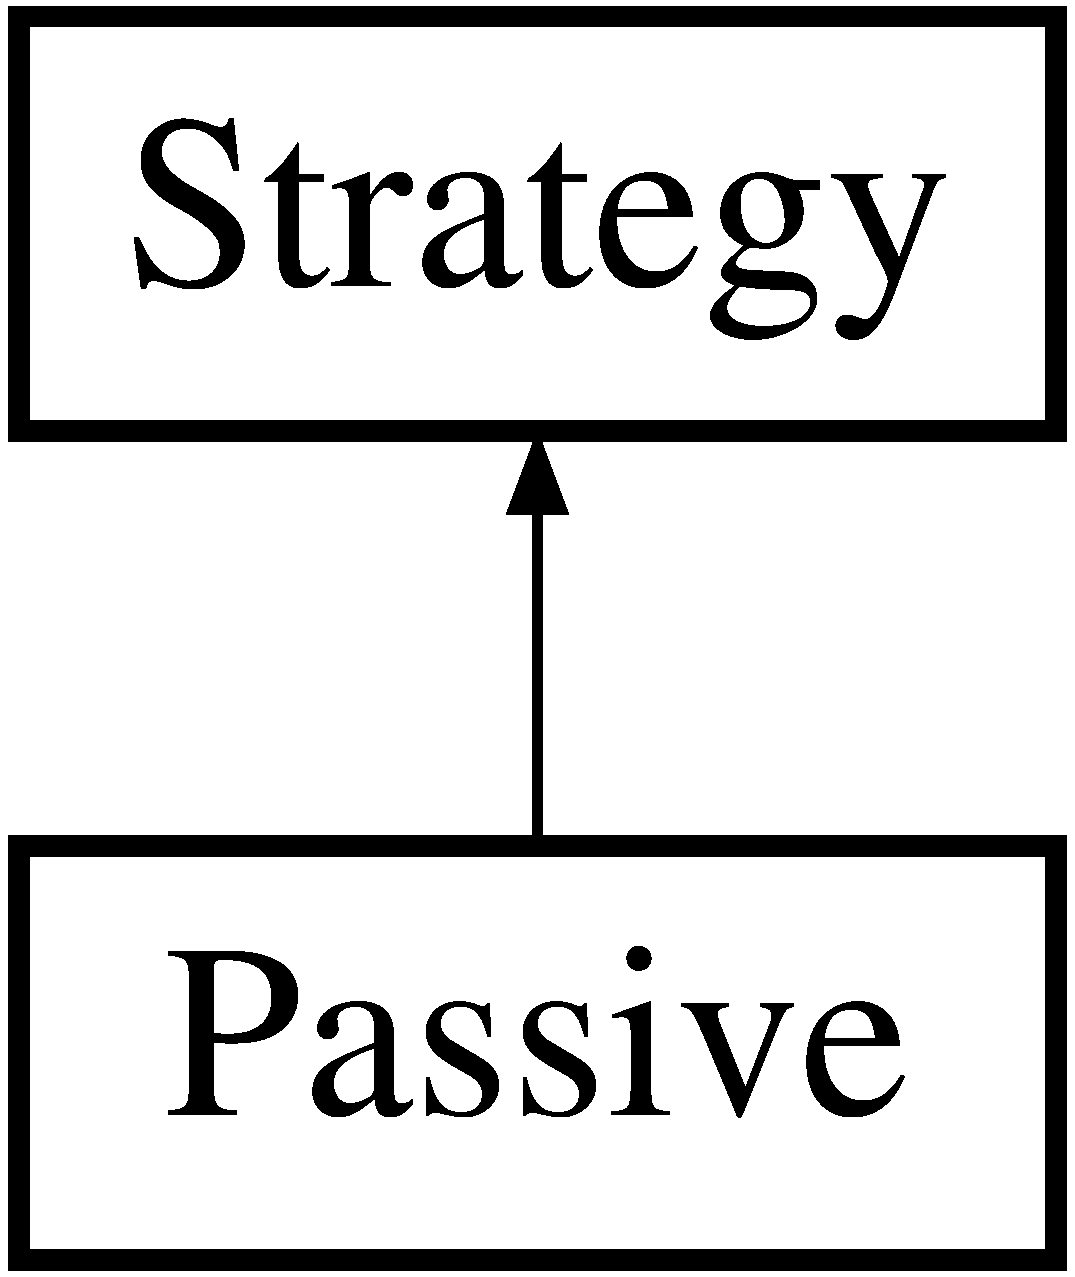
\includegraphics[height=2.000000cm]{classPassive}
\end{center}
\end{figure}
\doxysubsection*{Public Member Functions}
\begin{DoxyCompactItemize}
\item 
\mbox{\Hypertarget{classPassive_a0c79f8054b32733fd6d1f7fac663170c}\label{classPassive_a0c79f8054b32733fd6d1f7fac663170c}} 
void {\bfseries perform\+Strat} (Keypoint $\ast$key\+Point)
\end{DoxyCompactItemize}


\doxysubsection{Detailed Description}


Definition at line 4 of file Passive.\+h.



The documentation for this class was generated from the following files\+:\begin{DoxyCompactItemize}
\item 
Passive.\+h\item 
Passive.\+cpp\end{DoxyCompactItemize}

\hypertarget{classPersonnel}{}\doxysection{Personnel Class Reference}
\label{classPersonnel}\index{Personnel@{Personnel}}
Inheritance diagram for Personnel\+:\begin{figure}[H]
\begin{center}
\leavevmode
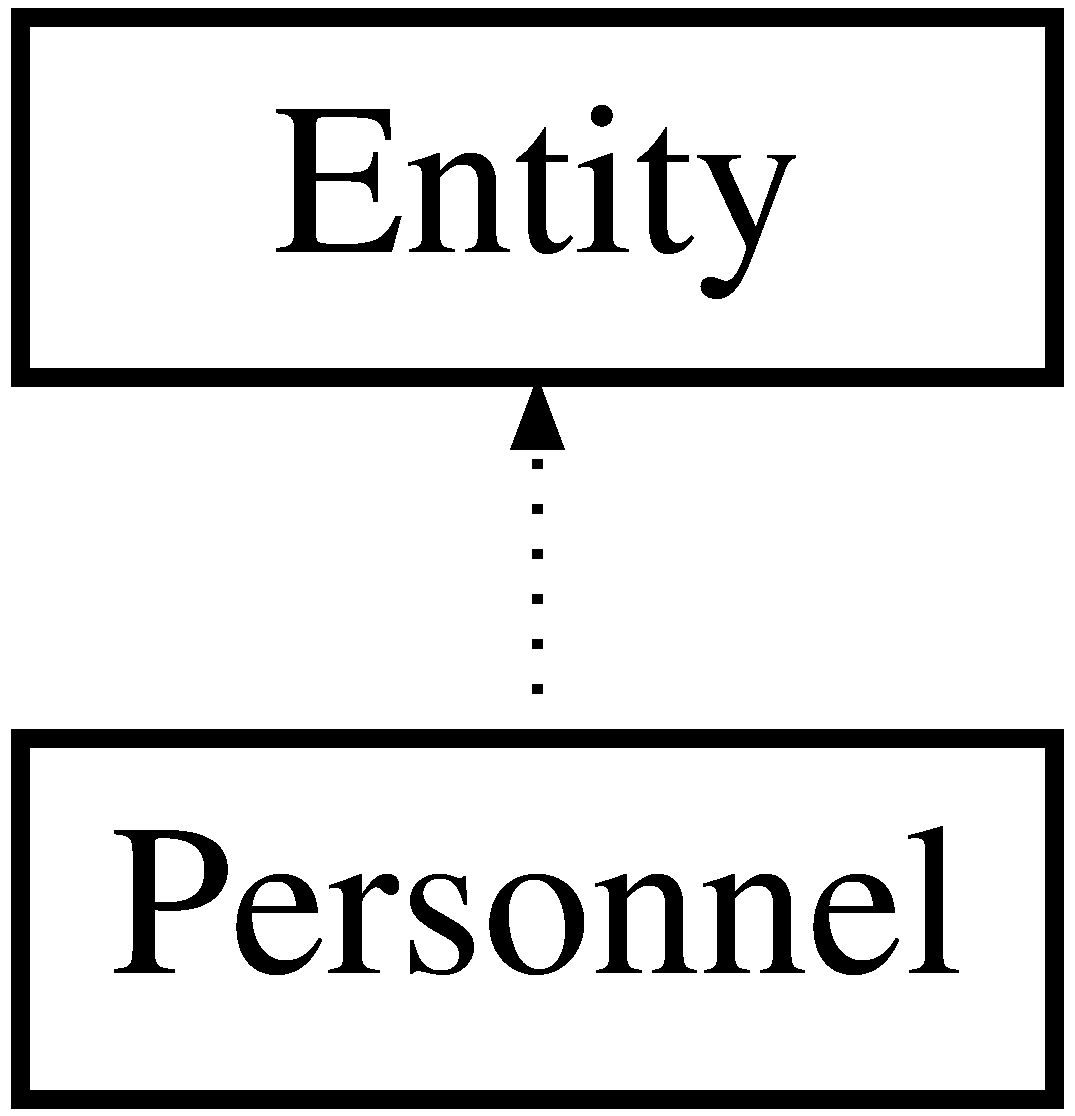
\includegraphics[height=2.000000cm]{classPersonnel}
\end{center}
\end{figure}
\doxysubsection*{Public Member Functions}
\begin{DoxyCompactItemize}
\item 
\mbox{\hyperlink{classPersonnel_a96840b35bd30d6010480a32cd296068b}{Personnel}} ()
\begin{DoxyCompactList}\small\item\em Instantiates the \mbox{\hyperlink{classPersonnel}{Personnel}}. \end{DoxyCompactList}\item 
void \mbox{\hyperlink{classPersonnel_aeb670c84c0168f872346c55f7fc8383f}{take\+Damage}} (int damage)
\begin{DoxyCompactList}\small\item\em Removes health from the \mbox{\hyperlink{classPersonnel}{Personnel}} object. \end{DoxyCompactList}\item 
void \mbox{\hyperlink{classPersonnel_af688c3cc32f413b1d17fe423f25aa50b}{deal\+Damage}} (\mbox{\hyperlink{classEntity}{Entity}} $\ast$entity)
\begin{DoxyCompactList}\small\item\em Inflicts damage onto another entity. \end{DoxyCompactList}\end{DoxyCompactItemize}


\doxysubsection{Detailed Description}


Definition at line 4 of file Personnel.\+h.



\doxysubsection{Constructor \& Destructor Documentation}
\mbox{\Hypertarget{classPersonnel_a96840b35bd30d6010480a32cd296068b}\label{classPersonnel_a96840b35bd30d6010480a32cd296068b}} 
\index{Personnel@{Personnel}!Personnel@{Personnel}}
\index{Personnel@{Personnel}!Personnel@{Personnel}}
\doxysubsubsection{\texorpdfstring{Personnel()}{Personnel()}}
{\footnotesize\ttfamily Personnel\+::\+Personnel (\begin{DoxyParamCaption}{ }\end{DoxyParamCaption})}



Instantiates the \mbox{\hyperlink{classPersonnel}{Personnel}}. 


\begin{DoxyParams}{Parameters}
{\em type} & must be a Type$\ast$ \\
\hline
\end{DoxyParams}


\doxysubsection{Member Function Documentation}
\mbox{\Hypertarget{classPersonnel_af688c3cc32f413b1d17fe423f25aa50b}\label{classPersonnel_af688c3cc32f413b1d17fe423f25aa50b}} 
\index{Personnel@{Personnel}!dealDamage@{dealDamage}}
\index{dealDamage@{dealDamage}!Personnel@{Personnel}}
\doxysubsubsection{\texorpdfstring{dealDamage()}{dealDamage()}}
{\footnotesize\ttfamily void Personnel\+::deal\+Damage (\begin{DoxyParamCaption}\item[{\mbox{\hyperlink{classEntity}{Entity}} $\ast$}]{entity }\end{DoxyParamCaption})\hspace{0.3cm}{\ttfamily [virtual]}}



Inflicts damage onto another entity. 

Preconditions\+:
\begin{DoxyItemize}
\item entity must be an Entity$\ast$
\end{DoxyItemize}

Postconditions\+:
\begin{DoxyItemize}
\item Reduces the health of the entity
\end{DoxyItemize}


\begin{DoxyParams}{Parameters}
{\em entity} & must be an Entity$\ast$ \\
\hline
\end{DoxyParams}
\begin{DoxyReturn}{Returns}
void 
\end{DoxyReturn}


Implements \mbox{\hyperlink{classEntity}{Entity}}.

\mbox{\Hypertarget{classPersonnel_aeb670c84c0168f872346c55f7fc8383f}\label{classPersonnel_aeb670c84c0168f872346c55f7fc8383f}} 
\index{Personnel@{Personnel}!takeDamage@{takeDamage}}
\index{takeDamage@{takeDamage}!Personnel@{Personnel}}
\doxysubsubsection{\texorpdfstring{takeDamage()}{takeDamage()}}
{\footnotesize\ttfamily void Personnel\+::take\+Damage (\begin{DoxyParamCaption}\item[{int}]{damage }\end{DoxyParamCaption})\hspace{0.3cm}{\ttfamily [virtual]}}



Removes health from the \mbox{\hyperlink{classPersonnel}{Personnel}} object. 

Preconditions\+:
\begin{DoxyItemize}
\item damage must be an int
\end{DoxyItemize}

Postconditions\+:
\begin{DoxyItemize}
\item Reduces the health of the \mbox{\hyperlink{classPersonnel}{Personnel}} object
\end{DoxyItemize}


\begin{DoxyParams}{Parameters}
{\em damage} & must be an int \\
\hline
\end{DoxyParams}
\begin{DoxyReturn}{Returns}
void 
\end{DoxyReturn}


Implements \mbox{\hyperlink{classEntity}{Entity}}.



The documentation for this class was generated from the following file\+:\begin{DoxyCompactItemize}
\item 
Personnel.\+h\end{DoxyCompactItemize}

\hypertarget{classPersonnelFactory}{}\section{Personnel\+Factory Class Reference}
\label{classPersonnelFactory}\index{Personnel\+Factory@{Personnel\+Factory}}


\hyperlink{classPersonnelFactory}{Personnel\+Factory} class.  




{\ttfamily \#include $<$Personnel\+Factory.\+h$>$}

Inheritance diagram for Personnel\+Factory\+:\begin{figure}[H]
\begin{center}
\leavevmode
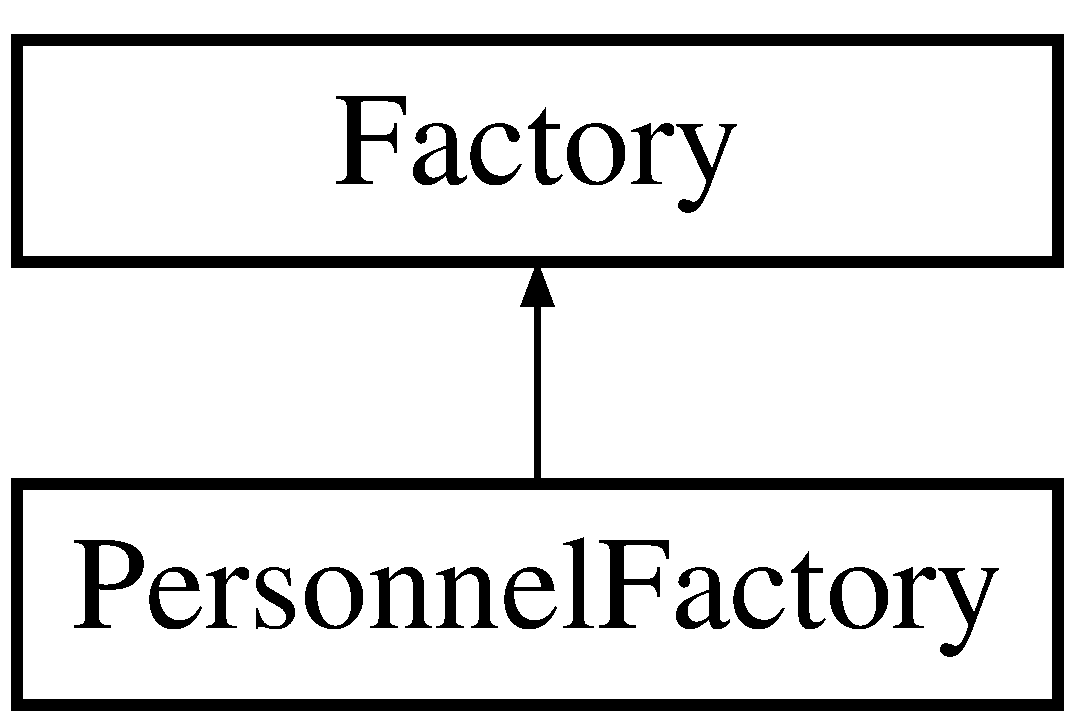
\includegraphics[height=2.000000cm]{classPersonnelFactory}
\end{center}
\end{figure}
\subsection*{Public Member Functions}
\begin{DoxyCompactItemize}
\item 
\hyperlink{classPersonnelFactory_a71cd406976230cacebfcfd723d2a2615}{Personnel\+Factory} (\hyperlink{classType}{Type} $\ast$type, \hyperlink{classAddOn}{Add\+On} $\ast$add\+On)
\begin{DoxyCompactList}\small\item\em Instantiates the \hyperlink{classPersonnel}{Personnel} factory. \end{DoxyCompactList}\item 
\hyperlink{classEntity}{Entity} $\ast$ \hyperlink{classPersonnelFactory_ae8684c246d5dfb1f469f368525867394}{create\+Entity} (\hyperlink{classAlliance}{Alliance} $\ast$alliance)
\begin{DoxyCompactList}\small\item\em Instantiates and returns a \hyperlink{classPersonnel}{Personnel} for the given alliance. \end{DoxyCompactList}\item 
\hyperlink{classFactory}{Factory} $\ast$ \hyperlink{classPersonnelFactory_ad60e8371e52153294112b16a7a97cc2d}{clone} ()
\begin{DoxyCompactList}\small\item\em Instantiates and returns a clone of the current \hyperlink{classPersonnel}{Personnel} factory. \end{DoxyCompactList}\end{DoxyCompactItemize}


\subsection{Detailed Description}
\hyperlink{classPersonnelFactory}{Personnel\+Factory} class. 

Used to instantiate \hyperlink{classPersonnel}{Personnel} objects. 

Definition at line 11 of file Personnel\+Factory.\+h.



\subsection{Constructor \& Destructor Documentation}
\mbox{\Hypertarget{classPersonnelFactory_a71cd406976230cacebfcfd723d2a2615}\label{classPersonnelFactory_a71cd406976230cacebfcfd723d2a2615}} 
\index{Personnel\+Factory@{Personnel\+Factory}!Personnel\+Factory@{Personnel\+Factory}}
\index{Personnel\+Factory@{Personnel\+Factory}!Personnel\+Factory@{Personnel\+Factory}}
\subsubsection{\texorpdfstring{Personnel\+Factory()}{PersonnelFactory()}}
{\footnotesize\ttfamily Personnel\+Factory\+::\+Personnel\+Factory (\begin{DoxyParamCaption}\item[{\hyperlink{classType}{Type} $\ast$}]{type,  }\item[{\hyperlink{classAddOn}{Add\+On} $\ast$}]{add\+On }\end{DoxyParamCaption})}



Instantiates the \hyperlink{classPersonnel}{Personnel} factory. 


\begin{DoxyParams}{Parameters}
{\em type} & must be a Type$\ast$ \\
\hline
{\em add\+On} & must be a Add\+On$\ast$ \\
\hline
\end{DoxyParams}


Definition at line 4 of file Personnel\+Factory.\+cpp.


\begin{DoxyCode}
4 : \hyperlink{classFactory_aca946f8877efb5b5bae700f74537d99d}{Factory}(type, addOn) \{\}
\end{DoxyCode}


\subsection{Member Function Documentation}
\mbox{\Hypertarget{classPersonnelFactory_ad60e8371e52153294112b16a7a97cc2d}\label{classPersonnelFactory_ad60e8371e52153294112b16a7a97cc2d}} 
\index{Personnel\+Factory@{Personnel\+Factory}!clone@{clone}}
\index{clone@{clone}!Personnel\+Factory@{Personnel\+Factory}}
\subsubsection{\texorpdfstring{clone()}{clone()}}
{\footnotesize\ttfamily \hyperlink{classFactory}{Factory} $\ast$ Personnel\+Factory\+::clone (\begin{DoxyParamCaption}{ }\end{DoxyParamCaption})\hspace{0.3cm}{\ttfamily [virtual]}}



Instantiates and returns a clone of the current \hyperlink{classPersonnel}{Personnel} factory. 

Postconditions\+:
\begin{DoxyItemize}
\item Returns the clone of the current \hyperlink{classPersonnel}{Personnel} factory
\end{DoxyItemize}

\begin{DoxyReturn}{Returns}
Factory$\ast$ The \hyperlink{classPersonnel}{Personnel} factory clone 
\end{DoxyReturn}


Implements \hyperlink{classFactory}{Factory}.



Definition at line 17 of file Personnel\+Factory.\+cpp.


\begin{DoxyCode}
17                                  \{
18     \textcolor{keywordflow}{return} \textcolor{keyword}{new} \hyperlink{classPersonnelFactory_a71cd406976230cacebfcfd723d2a2615}{PersonnelFactory}(\hyperlink{classFactory_ac91051006ace7ec5bb6ecf0fe6d02d58}{getType}(), \hyperlink{classFactory_a994153930f59cafb280e91d5b100b5aa}{getAddOn}());
19 \}
\end{DoxyCode}
\mbox{\Hypertarget{classPersonnelFactory_ae8684c246d5dfb1f469f368525867394}\label{classPersonnelFactory_ae8684c246d5dfb1f469f368525867394}} 
\index{Personnel\+Factory@{Personnel\+Factory}!create\+Entity@{create\+Entity}}
\index{create\+Entity@{create\+Entity}!Personnel\+Factory@{Personnel\+Factory}}
\subsubsection{\texorpdfstring{create\+Entity()}{createEntity()}}
{\footnotesize\ttfamily \hyperlink{classEntity}{Entity} $\ast$ Personnel\+Factory\+::create\+Entity (\begin{DoxyParamCaption}\item[{\hyperlink{classAlliance}{Alliance} $\ast$}]{alliance }\end{DoxyParamCaption})\hspace{0.3cm}{\ttfamily [virtual]}}



Instantiates and returns a \hyperlink{classPersonnel}{Personnel} for the given alliance. 

Preconditions\+:
\begin{DoxyItemize}
\item alliance must be an Alliance$\ast$
\end{DoxyItemize}

Postconditions\+:
\begin{DoxyItemize}
\item Returns the instantiated \hyperlink{classPersonnel}{Personnel} object with specific state
\end{DoxyItemize}


\begin{DoxyParams}{Parameters}
{\em alliance} & must be a Alliance$\ast$ \\
\hline
\end{DoxyParams}
\begin{DoxyReturn}{Returns}
Entity$\ast$ The instatiated personnel 
\end{DoxyReturn}


Implements \hyperlink{classFactory}{Factory}.



Definition at line 6 of file Personnel\+Factory.\+cpp.


\begin{DoxyCode}
6                                                          \{
7     \hyperlink{classPersonnel}{Personnel}* p = \textcolor{keyword}{new} \hyperlink{classPersonnel}{Personnel}(\hyperlink{classFactory_ac91051006ace7ec5bb6ecf0fe6d02d58}{getType}()->\hyperlink{classPersonnelFactory_ad60e8371e52153294112b16a7a97cc2d}{clone}());
8     \textcolor{keywordflow}{if} (\hyperlink{classFactory_a994153930f59cafb280e91d5b100b5aa}{getAddOn}() != NULL) \{
9         \hyperlink{classAddOn}{AddOn}* personnelAddOn = \hyperlink{classFactory_a994153930f59cafb280e91d5b100b5aa}{getAddOn}()->clone();
10         personnelAddOn->connectEntity(p);
11         \textcolor{keywordflow}{return} personnelAddOn;
12     \} \textcolor{keywordflow}{else} \{
13         \textcolor{keywordflow}{return} p;
14     \}
15 \}
\end{DoxyCode}


The documentation for this class was generated from the following files\+:\begin{DoxyCompactItemize}
\item 
Personnel\+Factory.\+h\item 
Personnel\+Factory.\+cpp\end{DoxyCompactItemize}

\hypertarget{classPiercing}{}\section{Piercing Class Reference}
\label{classPiercing}\index{Piercing@{Piercing}}


\hyperlink{classPiercing}{Piercing} class.  




{\ttfamily \#include $<$Piercing.\+h$>$}

Inheritance diagram for Piercing\+:\begin{figure}[H]
\begin{center}
\leavevmode
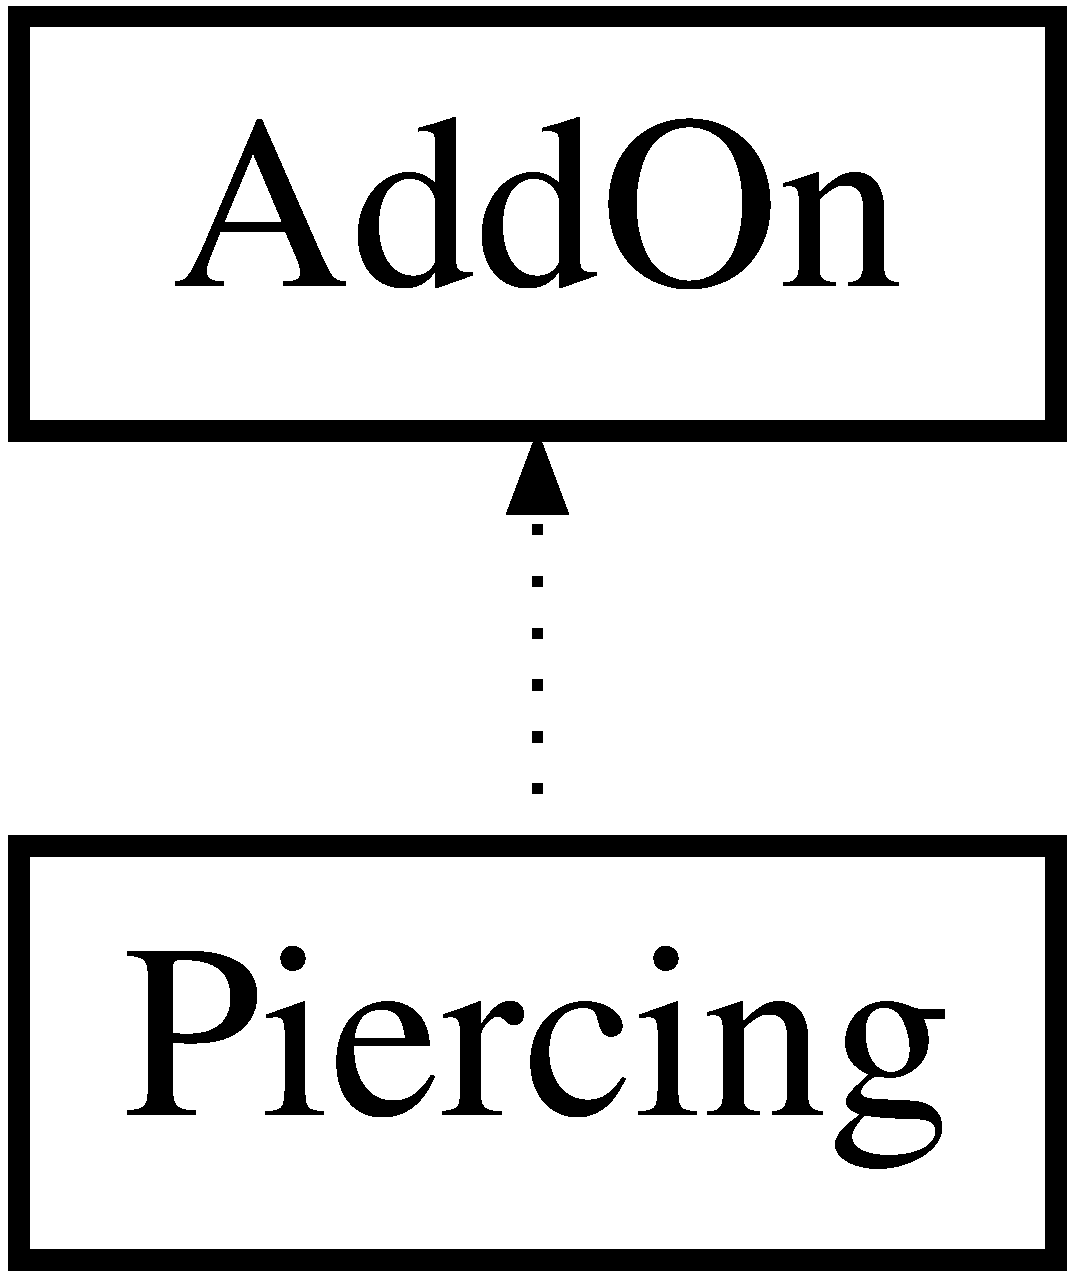
\includegraphics[height=2.000000cm]{classPiercing}
\end{center}
\end{figure}
\subsection*{Public Member Functions}
\begin{DoxyCompactItemize}
\item 
\hyperlink{classPiercing_a45a6d5d3b6e7ac24ebba63e56246d887}{Piercing} (\hyperlink{classEntity}{Entity} $\ast$entity, int value)
\begin{DoxyCompactList}\small\item\em Instantiates an \hyperlink{classPiercing}{Piercing}. \end{DoxyCompactList}\item 
void \hyperlink{classPiercing_a103634469a43e1662bd5e07e66901667}{take\+Damage} (int damage)
\begin{DoxyCompactList}\small\item\em Decreases the entities\textquotesingle{} armour value (or health when their armour has depleted) \end{DoxyCompactList}\item 
void \hyperlink{classPiercing_a2dbd4a497f9abbebbbd2ceb2909f6163}{deal\+Damage} (\hyperlink{classEntity}{Entity} $\ast$entity)
\begin{DoxyCompactList}\small\item\em Adds to the damage \hyperlink{classEntity}{Entity} objects inflict. \end{DoxyCompactList}\end{DoxyCompactItemize}


\subsection{Detailed Description}
\hyperlink{classPiercing}{Piercing} class. 

Used to add to the damage \hyperlink{classEntity}{Entity} objects inflict. 

Definition at line 9 of file Piercing.\+h.



\subsection{Constructor \& Destructor Documentation}
\mbox{\Hypertarget{classPiercing_a45a6d5d3b6e7ac24ebba63e56246d887}\label{classPiercing_a45a6d5d3b6e7ac24ebba63e56246d887}} 
\index{Piercing@{Piercing}!Piercing@{Piercing}}
\index{Piercing@{Piercing}!Piercing@{Piercing}}
\subsubsection{\texorpdfstring{Piercing()}{Piercing()}}
{\footnotesize\ttfamily Piercing\+::\+Piercing (\begin{DoxyParamCaption}\item[{\hyperlink{classEntity}{Entity} $\ast$}]{entity,  }\item[{int}]{value }\end{DoxyParamCaption})}



Instantiates an \hyperlink{classPiercing}{Piercing}. 


\begin{DoxyParams}{Parameters}
{\em entity} & must be a Entity$\ast$ \\
\hline
{\em value} & must be a int \\
\hline
\end{DoxyParams}


Definition at line 4 of file Piercing.\+cpp.


\begin{DoxyCode}
4                                             \{
5     \textcolor{comment}{// TODO - implement Piercing::Piercing}
6     \textcolor{keywordflow}{throw} \textcolor{stringliteral}{"Not yet implemented"};
7 \}
\end{DoxyCode}


\subsection{Member Function Documentation}
\mbox{\Hypertarget{classPiercing_a2dbd4a497f9abbebbbd2ceb2909f6163}\label{classPiercing_a2dbd4a497f9abbebbbd2ceb2909f6163}} 
\index{Piercing@{Piercing}!deal\+Damage@{deal\+Damage}}
\index{deal\+Damage@{deal\+Damage}!Piercing@{Piercing}}
\subsubsection{\texorpdfstring{deal\+Damage()}{dealDamage()}}
{\footnotesize\ttfamily void Piercing\+::deal\+Damage (\begin{DoxyParamCaption}\item[{\hyperlink{classEntity}{Entity} $\ast$}]{entity }\end{DoxyParamCaption})\hspace{0.3cm}{\ttfamily [virtual]}}



Adds to the damage \hyperlink{classEntity}{Entity} objects inflict. 

Preconditions\+:
\begin{DoxyItemize}
\item entity must be an Entity$\ast$
\end{DoxyItemize}

Postconditions\+:
\begin{DoxyItemize}
\item Inflicts damage to passed in \hyperlink{classEntity}{Entity} objects using the sum of it\textquotesingle{}s value and the entity onto which it has been added\textquotesingle{}s value
\end{DoxyItemize}


\begin{DoxyParams}{Parameters}
{\em entity} & must be an Entity$\ast$ \\
\hline
\end{DoxyParams}
\begin{DoxyReturn}{Returns}
void 
\end{DoxyReturn}


Implements \hyperlink{classAddOn}{Add\+On}.



Definition at line 14 of file Piercing.\+cpp.


\begin{DoxyCode}
14                                         \{
15     \textcolor{comment}{// TODO - implement Piercing::dealDamage}
16     \textcolor{keywordflow}{throw} \textcolor{stringliteral}{"Not yet implemented"};
17 \}
\end{DoxyCode}
\mbox{\Hypertarget{classPiercing_a103634469a43e1662bd5e07e66901667}\label{classPiercing_a103634469a43e1662bd5e07e66901667}} 
\index{Piercing@{Piercing}!take\+Damage@{take\+Damage}}
\index{take\+Damage@{take\+Damage}!Piercing@{Piercing}}
\subsubsection{\texorpdfstring{take\+Damage()}{takeDamage()}}
{\footnotesize\ttfamily void Piercing\+::take\+Damage (\begin{DoxyParamCaption}\item[{int}]{damage }\end{DoxyParamCaption})\hspace{0.3cm}{\ttfamily [virtual]}}



Decreases the entities\textquotesingle{} armour value (or health when their armour has depleted) 

Preconditions\+:
\begin{DoxyItemize}
\item damage must be an int
\end{DoxyItemize}

Postconditions\+:
\begin{DoxyItemize}
\item Does nothing
\end{DoxyItemize}


\begin{DoxyParams}{Parameters}
{\em damage} & must be an int \\
\hline
\end{DoxyParams}
\begin{DoxyReturn}{Returns}
void 
\end{DoxyReturn}


Implements \hyperlink{classAddOn}{Add\+On}.



Definition at line 9 of file Piercing.\+cpp.


\begin{DoxyCode}
9                                     \{
10     \textcolor{comment}{// TODO - implement Piercing::takeDamage}
11     \textcolor{keywordflow}{throw} \textcolor{stringliteral}{"Not yet implemented"};
12 \}
\end{DoxyCode}


The documentation for this class was generated from the following files\+:\begin{DoxyCompactItemize}
\item 
Piercing.\+h\item 
Piercing.\+cpp\end{DoxyCompactItemize}

\hypertarget{classRainy}{}\doxysection{Rainy Class Reference}
\label{classRainy}\index{Rainy@{Rainy}}
Inheritance diagram for Rainy\+:\begin{figure}[H]
\begin{center}
\leavevmode
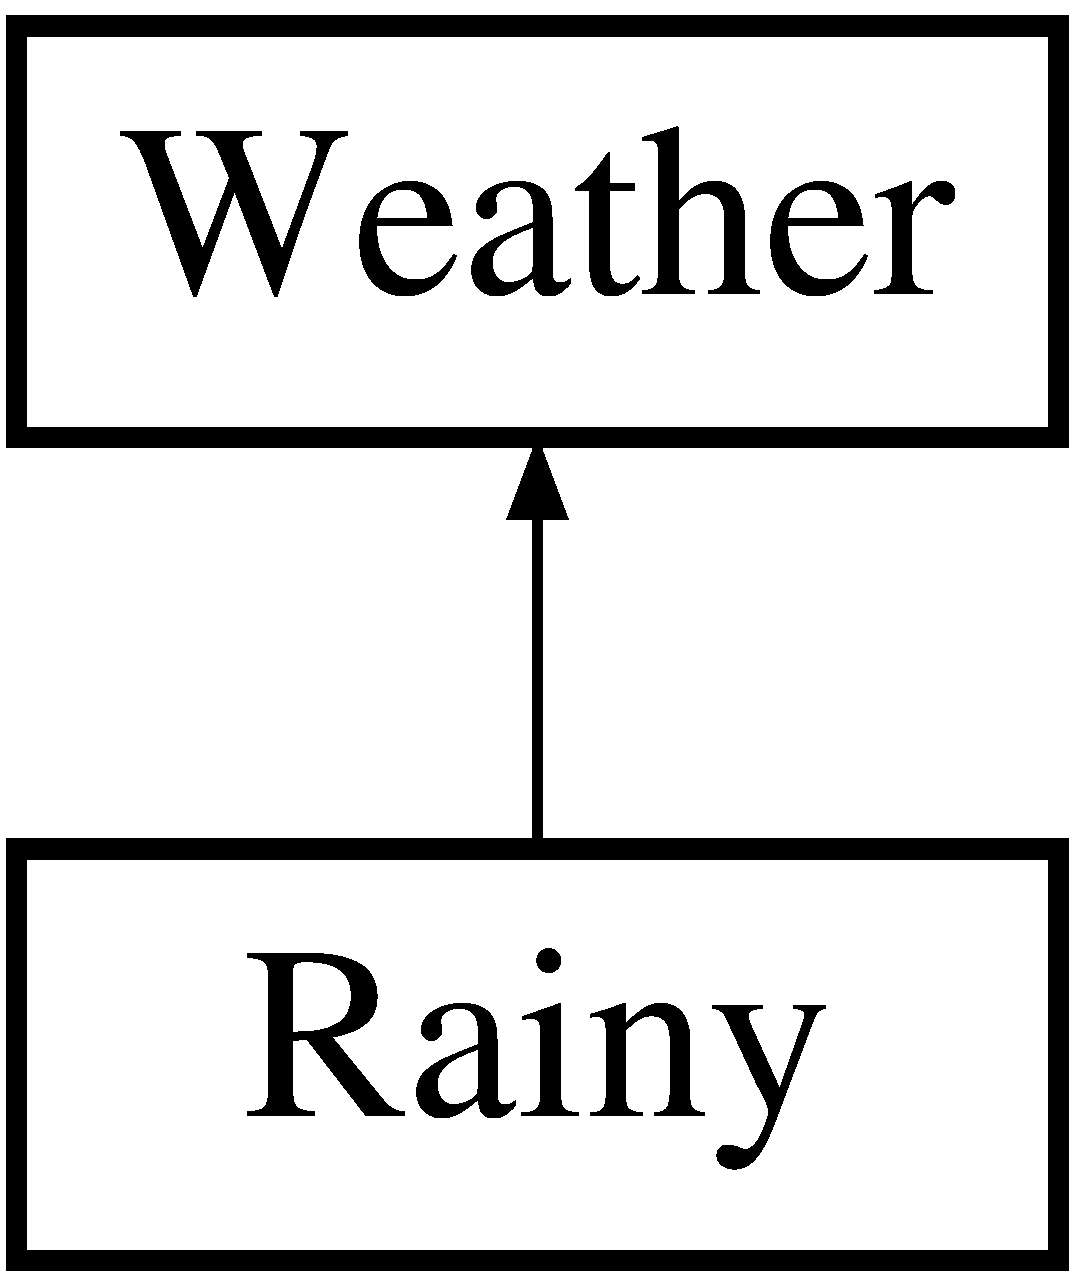
\includegraphics[height=2.000000cm]{classRainy}
\end{center}
\end{figure}
\doxysubsection*{Public Member Functions}
\begin{DoxyCompactItemize}
\item 
\mbox{\hyperlink{classRainy_aae3bc68f19aacf2a863e9524b0b3e302}{Rainy}} ()
\begin{DoxyCompactList}\small\item\em Instantiates the Runny object of the state pattern. \end{DoxyCompactList}\item 
<<<<<<< HEAD
<<<<<<< HEAD
<<<<<<< HEAD
std\+::string \hyperlink{classRainy_adc4d5851d1e9efd45b153ae0d5ead832}{get\+Weather} ()
\begin{DoxyCompactList}\small\item\em Returns string which tels us the weather. \end{DoxyCompactList}\item 
void \hyperlink{classRainy_ac0ed80bde42f58ff16a9ee4941b85ef9}{handle\+Change} (\hyperlink{classKeyPoint}{Key\+Point} $\ast$keypoint)
\begin{DoxyCompactList}\small\item\em Will change the current state of the weather inside the specific keypoint. \end{DoxyCompactList}\end{DoxyCompactItemize}
\subsection*{Additional Inherited Members}
=======
std\+::string \mbox{\hyperlink{classRainy_adc4d5851d1e9efd45b153ae0d5ead832}{get\+Weather}} ()
\begin{DoxyCompactList}\small\item\em Returns string which tels us the weather. \end{DoxyCompactList}\item 
=======
std\+::string \mbox{\hyperlink{classRainy_adc4d5851d1e9efd45b153ae0d5ead832}{get\+Weather}} ()
\begin{DoxyCompactList}\small\item\em Returns string which tels us the weather. \end{DoxyCompactList}\item 
>>>>>>> 7be49738cebc0ced3357f2ce74f6fda2ea0b3d5e
=======
std\+::string \mbox{\hyperlink{classRainy_adc4d5851d1e9efd45b153ae0d5ead832}{get\+Weather}} ()
\begin{DoxyCompactList}\small\item\em Returns string which tels us the weather. \end{DoxyCompactList}\item 
>>>>>>> 7be49738cebc0ced3357f2ce74f6fda2ea0b3d5e
void \mbox{\hyperlink{classRainy_a723a0dce680b6de43aaf6569a2e2a4d8}{handle\+Change}} (\mbox{\hyperlink{classKeyPoint}{Key\+Point}} $\ast$k)
\begin{DoxyCompactList}\small\item\em Will change the current state of the weather inside the specific keypoint. \end{DoxyCompactList}\item 
\mbox{\hyperlink{classWeather}{Weather}} $\ast$ \mbox{\hyperlink{classRainy_a30adf6c86ad1dab6089e90a16b5d0753}{clone}} ()
\begin{DoxyCompactList}\small\item\em Returns a clone of the \mbox{\hyperlink{classRainy}{Rainy}} object. \end{DoxyCompactList}\end{DoxyCompactItemize}
\doxysubsection*{Additional Inherited Members}
<<<<<<< HEAD
<<<<<<< HEAD
>>>>>>> 7be49738cebc0ced3357f2ce74f6fda2ea0b3d5e
=======
>>>>>>> 7be49738cebc0ced3357f2ce74f6fda2ea0b3d5e
=======
>>>>>>> 7be49738cebc0ced3357f2ce74f6fda2ea0b3d5e


\doxysubsection{Detailed Description}


Definition at line \mbox{\hyperlink{Rainy_8h_source_l00006}{6}} of file \mbox{\hyperlink{Rainy_8h_source}{Rainy.\+h}}.



<<<<<<< HEAD
<<<<<<< HEAD
<<<<<<< HEAD
\subsection{Member Function Documentation}
\mbox{\Hypertarget{classRainy_adc4d5851d1e9efd45b153ae0d5ead832}\label{classRainy_adc4d5851d1e9efd45b153ae0d5ead832}} 
\index{Rainy@{Rainy}!get\+Weather@{get\+Weather}}
\index{get\+Weather@{get\+Weather}!Rainy@{Rainy}}
\subsubsection{\texorpdfstring{get\+Weather()}{getWeather()}}
=======
=======
>>>>>>> 7be49738cebc0ced3357f2ce74f6fda2ea0b3d5e
=======
>>>>>>> 7be49738cebc0ced3357f2ce74f6fda2ea0b3d5e
\doxysubsection{Constructor \& Destructor Documentation}
\mbox{\Hypertarget{classRainy_aae3bc68f19aacf2a863e9524b0b3e302}\label{classRainy_aae3bc68f19aacf2a863e9524b0b3e302}} 
\index{Rainy@{Rainy}!Rainy@{Rainy}}
\index{Rainy@{Rainy}!Rainy@{Rainy}}
\doxysubsubsection{\texorpdfstring{Rainy()}{Rainy()}}
{\footnotesize\ttfamily Rainy\+::\+Rainy (\begin{DoxyParamCaption}{ }\end{DoxyParamCaption})}



Instantiates the Runny object of the state pattern. 



Definition at line \mbox{\hyperlink{Rainy_8cpp_source_l00004}{4}} of file \mbox{\hyperlink{Rainy_8cpp_source}{Rainy.\+cpp}}.


\begin{DoxyCode}{0}
\DoxyCodeLine{00004             : \mbox{\hyperlink{classWeather_aa404c94fec05b825454a7309827767c6}{Weather}}() \{}
\DoxyCodeLine{00005     this-\/>multiplier = 0.5;}
\DoxyCodeLine{00006 \}}

\end{DoxyCode}


\doxysubsection{Member Function Documentation}
\mbox{\Hypertarget{classRainy_a30adf6c86ad1dab6089e90a16b5d0753}\label{classRainy_a30adf6c86ad1dab6089e90a16b5d0753}} 
\index{Rainy@{Rainy}!clone@{clone}}
\index{clone@{clone}!Rainy@{Rainy}}
\doxysubsubsection{\texorpdfstring{clone()}{clone()}}
{\footnotesize\ttfamily \mbox{\hyperlink{classWeather}{Weather}} $\ast$ Rainy\+::clone (\begin{DoxyParamCaption}{ }\end{DoxyParamCaption})\hspace{0.3cm}{\ttfamily [virtual]}}



Returns a clone of the \mbox{\hyperlink{classRainy}{Rainy}} object. 

\begin{DoxyReturn}{Returns}
Weather$\ast$ The clone of the rainy object 
\end{DoxyReturn}


Implements \mbox{\hyperlink{classWeather}{Weather}}.



Definition at line \mbox{\hyperlink{Rainy_8cpp_source_l00017}{17}} of file \mbox{\hyperlink{Rainy_8cpp_source}{Rainy.\+cpp}}.


\begin{DoxyCode}{0}
\DoxyCodeLine{00017                       \{}
\DoxyCodeLine{00018     \textcolor{keywordflow}{return} \textcolor{keyword}{new} \mbox{\hyperlink{classRainy_aae3bc68f19aacf2a863e9524b0b3e302}{Rainy}}();}
\DoxyCodeLine{00019 \}}

\end{DoxyCode}
\mbox{\Hypertarget{classRainy_adc4d5851d1e9efd45b153ae0d5ead832}\label{classRainy_adc4d5851d1e9efd45b153ae0d5ead832}} 
\index{Rainy@{Rainy}!getWeather@{getWeather}}
\index{getWeather@{getWeather}!Rainy@{Rainy}}
\doxysubsubsection{\texorpdfstring{getWeather()}{getWeather()}}
<<<<<<< HEAD
<<<<<<< HEAD
>>>>>>> 7be49738cebc0ced3357f2ce74f6fda2ea0b3d5e
=======
>>>>>>> 7be49738cebc0ced3357f2ce74f6fda2ea0b3d5e
=======
>>>>>>> 7be49738cebc0ced3357f2ce74f6fda2ea0b3d5e
{\footnotesize\ttfamily std\+::string Rainy\+::get\+Weather (\begin{DoxyParamCaption}{ }\end{DoxyParamCaption})\hspace{0.3cm}{\ttfamily [virtual]}}



Returns string which tels us the weather. 

Postconditions\+:
\begin{DoxyItemize}
\item Returns the wether of ths current state
\end{DoxyItemize}

\begin{DoxyReturn}{Returns}
std\+::string which is the current state 
\end{DoxyReturn}


<<<<<<< HEAD
<<<<<<< HEAD
<<<<<<< HEAD
Implements \hyperlink{classWeather_ad0a29227308b87e98808cdff52232df3}{Weather}.



Definition at line 8 of file Rainy.\+cpp.


\begin{DoxyCode}
8                             \{
9     \textcolor{keywordflow}{return} \textcolor{stringliteral}{"Rainy"};
10 \}
\end{DoxyCode}
\mbox{\Hypertarget{classRainy_ac0ed80bde42f58ff16a9ee4941b85ef9}\label{classRainy_ac0ed80bde42f58ff16a9ee4941b85ef9}} 
\index{Rainy@{Rainy}!handle\+Change@{handle\+Change}}
\index{handle\+Change@{handle\+Change}!Rainy@{Rainy}}
\subsubsection{\texorpdfstring{handle\+Change()}{handleChange()}}
{\footnotesize\ttfamily void Rainy\+::handle\+Change (\begin{DoxyParamCaption}\item[{\hyperlink{classKeyPoint}{Key\+Point} $\ast$}]{keypoint }\end{DoxyParamCaption})\hspace{0.3cm}{\ttfamily [virtual]}}
=======
Implements \mbox{\hyperlink{classWeather}{Weather}}.



=======
Implements \mbox{\hyperlink{classWeather}{Weather}}.



>>>>>>> 7be49738cebc0ced3357f2ce74f6fda2ea0b3d5e
=======
Implements \mbox{\hyperlink{classWeather}{Weather}}.



>>>>>>> 7be49738cebc0ced3357f2ce74f6fda2ea0b3d5e
Definition at line \mbox{\hyperlink{Rainy_8cpp_source_l00008}{8}} of file \mbox{\hyperlink{Rainy_8cpp_source}{Rainy.\+cpp}}.


\begin{DoxyCode}{0}
\DoxyCodeLine{00008                             \{}
\DoxyCodeLine{00009     \textcolor{keywordflow}{return} \textcolor{stringliteral}{"{}Rainy"{}};}
\DoxyCodeLine{00010 \}}

\end{DoxyCode}
\mbox{\Hypertarget{classRainy_a723a0dce680b6de43aaf6569a2e2a4d8}\label{classRainy_a723a0dce680b6de43aaf6569a2e2a4d8}} 
\index{Rainy@{Rainy}!handleChange@{handleChange}}
\index{handleChange@{handleChange}!Rainy@{Rainy}}
\doxysubsubsection{\texorpdfstring{handleChange()}{handleChange()}}
{\footnotesize\ttfamily void Rainy\+::handle\+Change (\begin{DoxyParamCaption}\item[{\mbox{\hyperlink{classKeyPoint}{Key\+Point}} $\ast$}]{k }\end{DoxyParamCaption})\hspace{0.3cm}{\ttfamily [virtual]}}
<<<<<<< HEAD
<<<<<<< HEAD
>>>>>>> 7be49738cebc0ced3357f2ce74f6fda2ea0b3d5e
=======
>>>>>>> 7be49738cebc0ced3357f2ce74f6fda2ea0b3d5e
=======
>>>>>>> 7be49738cebc0ced3357f2ce74f6fda2ea0b3d5e



Will change the current state of the weather inside the specific keypoint. 

Preconditions\+:
\begin{DoxyItemize}
\item keypoint must be a Key\+Point$\ast$
\end{DoxyItemize}

Postconditions\+:
\begin{DoxyItemize}
\item Changes the current weather to the next one in the state pattern (\mbox{\hyperlink{classSunny}{Sunny}})
\end{DoxyItemize}


\begin{DoxyParams}{Parameters}
{\em keypoint} & must be a Key\+Point$\ast$ \\
\hline
\end{DoxyParams}
\begin{DoxyReturn}{Returns}
void 
\end{DoxyReturn}


<<<<<<< HEAD
<<<<<<< HEAD
<<<<<<< HEAD
Implements \hyperlink{classWeather_afc84c48c326fc967915833e689bfa40c}{Weather}.



Definition at line 12 of file Rainy.\+cpp.


\begin{DoxyCode}
12                                            \{
13     \hyperlink{classSunny}{Sunny}* newWeather = \textcolor{keyword}{new} \hyperlink{classSunny}{Sunny}();
14     keypoint->\hyperlink{classKeyPoint_a5c4b9314440a00fca7ab4d82ea4693a5}{setWeather}(newWeather);
15 \}
=======
Implements \mbox{\hyperlink{classWeather}{Weather}}.



=======
Implements \mbox{\hyperlink{classWeather}{Weather}}.



>>>>>>> 7be49738cebc0ced3357f2ce74f6fda2ea0b3d5e
=======
Implements \mbox{\hyperlink{classWeather}{Weather}}.



>>>>>>> 7be49738cebc0ced3357f2ce74f6fda2ea0b3d5e
Definition at line \mbox{\hyperlink{Rainy_8cpp_source_l00012}{12}} of file \mbox{\hyperlink{Rainy_8cpp_source}{Rainy.\+cpp}}.


\begin{DoxyCode}{0}
\DoxyCodeLine{00012                                     \{}
\DoxyCodeLine{00013     \mbox{\hyperlink{classSunny}{Sunny}}* newWeather = \textcolor{keyword}{new} \mbox{\hyperlink{classSunny}{Sunny}}();}
\DoxyCodeLine{00014     k-\/>\mbox{\hyperlink{classKeyPoint_a5c4b9314440a00fca7ab4d82ea4693a5}{setWeather}}(newWeather);}
\DoxyCodeLine{00015 \}}

<<<<<<< HEAD
<<<<<<< HEAD
>>>>>>> 7be49738cebc0ced3357f2ce74f6fda2ea0b3d5e
=======
>>>>>>> 7be49738cebc0ced3357f2ce74f6fda2ea0b3d5e
=======
>>>>>>> 7be49738cebc0ced3357f2ce74f6fda2ea0b3d5e
\end{DoxyCode}


The documentation for this class was generated from the following files\+:\begin{DoxyCompactItemize}
\item 
Rainy.\+h\item 
Rainy.\+cpp\end{DoxyCompactItemize}

<<<<<<< HEAD
\hypertarget{classSaveArchive}{}\section{Save\+Archive Class Reference}
\label{classSaveArchive}\index{Save\+Archive@{Save\+Archive}}
=======
\hypertarget{classSaveArchive}{}\doxysection{Save\+Archive Class Reference}
\label{classSaveArchive}\index{SaveArchive@{SaveArchive}}
>>>>>>> 7be49738cebc0ced3357f2ce74f6fda2ea0b3d5e


Stores a list of mementos containing simulation state.  




{\ttfamily \#include $<$Save\+Archive.\+h$>$}

<<<<<<< HEAD
\subsection*{Public Member Functions}
\begin{DoxyCompactItemize}
\item 
\mbox{\Hypertarget{classSaveArchive_a676252cf830fbe7b2a2b37ce2371a859}\label{classSaveArchive_a676252cf830fbe7b2a2b37ce2371a859}} 
\hyperlink{classSaveArchive_a676252cf830fbe7b2a2b37ce2371a859}{Save\+Archive} ()
\begin{DoxyCompactList}\small\item\em Instantiates the \hyperlink{classSaveArchive}{Save\+Archive} class. \end{DoxyCompactList}\item 
void \hyperlink{classSaveArchive_ab6927785f5b7f07b079a424773796d49}{add\+New\+Save} (std\+::string new\+Save\+Name, \hyperlink{classWarEngineMemento}{War\+Engine\+Memento} $\ast$new\+Save)
\begin{DoxyCompactList}\small\item\em Adds a new save to the list of stored mementos. \end{DoxyCompactList}\item 
\hyperlink{classWarEngineMemento}{War\+Engine\+Memento} $\ast$ \hyperlink{classSaveArchive_a144c8a27272d190164ad1f0e9dbdcc01}{get\+Last\+Save} ()
\begin{DoxyCompactList}\small\item\em Returns the last saved memento. \end{DoxyCompactList}\item 
\hyperlink{classWarEngineMemento}{War\+Engine\+Memento} $\ast$ \hyperlink{classSaveArchive_ad65ce77b8a9027b4e4a5d67ca1f06877}{get\+Save} (std\+::string name)
\begin{DoxyCompactList}\small\item\em Returns the last saved memento. Preconditions\+: \end{DoxyCompactList}\item 
void \hyperlink{classSaveArchive_a70c8ccaf0ac543dd8d4474f2f6383b35}{clear\+Save\+List} ()
\begin{DoxyCompactList}\small\item\em Erases all saved mementos from the list of saves. Postconditions\+: \end{DoxyCompactList}\item 
void \hyperlink{classSaveArchive_a416beb211cd59fed04df7347ebe41f36}{delete\+Save} (std\+::string name)
\begin{DoxyCompactList}\small\item\em Deletes a memento with the matching given name from the list of saved mementos. Preconditions\+: \end{DoxyCompactList}\end{DoxyCompactItemize}


\subsection{Detailed Description}
Stores a list of mementos containing simulation state. 

Definition at line 11 of file Save\+Archive.\+h.


=======
\doxysubsection*{Public Member Functions}
\begin{DoxyCompactItemize}
\item 
\mbox{\hyperlink{classSaveArchive_a676252cf830fbe7b2a2b37ce2371a859}{Save\+Archive}} ()
\begin{DoxyCompactList}\small\item\em Instantiates the \mbox{\hyperlink{classSaveArchive}{Save\+Archive}} class. \end{DoxyCompactList}\item 
void \mbox{\hyperlink{classSaveArchive_ab6927785f5b7f07b079a424773796d49}{add\+New\+Save}} (std\+::string new\+Save\+Name, \mbox{\hyperlink{classWarEngineMemento}{War\+Engine\+Memento}} $\ast$new\+Save)
\begin{DoxyCompactList}\small\item\em Adds a new save to the list of stored mementos. \end{DoxyCompactList}\item 
\mbox{\hyperlink{classWarEngineMemento}{War\+Engine\+Memento}} $\ast$ \mbox{\hyperlink{classSaveArchive_a144c8a27272d190164ad1f0e9dbdcc01}{get\+Last\+Save}} ()
\begin{DoxyCompactList}\small\item\em Returns the last saved memento. \end{DoxyCompactList}\item 
\mbox{\hyperlink{classWarEngineMemento}{War\+Engine\+Memento}} $\ast$ \mbox{\hyperlink{classSaveArchive_ad65ce77b8a9027b4e4a5d67ca1f06877}{get\+Save}} (std\+::string name)
\begin{DoxyCompactList}\small\item\em Returns the last saved memento. Preconditions\+: \end{DoxyCompactList}\item 
void \mbox{\hyperlink{classSaveArchive_a70c8ccaf0ac543dd8d4474f2f6383b35}{clear\+Save\+List}} ()
\begin{DoxyCompactList}\small\item\em Erases all saved mementos from the list of saves. Postconditions\+: \end{DoxyCompactList}\item 
void \mbox{\hyperlink{classSaveArchive_a416beb211cd59fed04df7347ebe41f36}{delete\+Save}} (std\+::string name)
\begin{DoxyCompactList}\small\item\em Deletes a memento with the matching given name from the list of saved mementos. Preconditions\+: \end{DoxyCompactList}\end{DoxyCompactItemize}


\doxysubsection{Detailed Description}
Stores a list of mementos containing simulation state. 

Definition at line \mbox{\hyperlink{SaveArchive_8h_source_l00011}{11}} of file \mbox{\hyperlink{SaveArchive_8h_source}{Save\+Archive.\+h}}.



\doxysubsection{Constructor \& Destructor Documentation}
\mbox{\Hypertarget{classSaveArchive_a676252cf830fbe7b2a2b37ce2371a859}\label{classSaveArchive_a676252cf830fbe7b2a2b37ce2371a859}} 
\index{SaveArchive@{SaveArchive}!SaveArchive@{SaveArchive}}
\index{SaveArchive@{SaveArchive}!SaveArchive@{SaveArchive}}
\doxysubsubsection{\texorpdfstring{SaveArchive()}{SaveArchive()}}
{\footnotesize\ttfamily Save\+Archive\+::\+Save\+Archive (\begin{DoxyParamCaption}{ }\end{DoxyParamCaption})}



Instantiates the \mbox{\hyperlink{classSaveArchive}{Save\+Archive}} class. 



Definition at line \mbox{\hyperlink{SaveArchive_8cpp_source_l00003}{3}} of file \mbox{\hyperlink{SaveArchive_8cpp_source}{Save\+Archive.\+cpp}}.


\begin{DoxyCode}{0}
\DoxyCodeLine{00003 \{\}}

\end{DoxyCode}


\doxysubsection{Member Function Documentation}
\mbox{\Hypertarget{classSaveArchive_ab6927785f5b7f07b079a424773796d49}\label{classSaveArchive_ab6927785f5b7f07b079a424773796d49}} 
\index{SaveArchive@{SaveArchive}!addNewSave@{addNewSave}}
\index{addNewSave@{addNewSave}!SaveArchive@{SaveArchive}}
\doxysubsubsection{\texorpdfstring{addNewSave()}{addNewSave()}}
{\footnotesize\ttfamily void Save\+Archive\+::add\+New\+Save (\begin{DoxyParamCaption}\item[{std\+::string}]{new\+Save\+Name,  }\item[{\mbox{\hyperlink{classWarEngineMemento}{War\+Engine\+Memento}} $\ast$}]{new\+Save }\end{DoxyParamCaption})}



Adds a new save to the list of stored mementos. 

Preconditions\+:
\begin{DoxyItemize}
\item new\+Save must be a War\+Engine\+Memento$\ast$
\item new\+Save\+Name must be a string
\end{DoxyItemize}

Postconditions\+:
\begin{DoxyItemize}
\item Adds a new memento to list of saves 
\begin{DoxyParams}{Parameters}
{\em new\+Save} & must be a War\+Engine\+Memento$\ast$ \\
\hline
{\em new\+Save\+Name} & must be a string \\
\hline
\end{DoxyParams}
\begin{DoxyReturn}{Returns}
void 
\end{DoxyReturn}

\end{DoxyItemize}

Definition at line \mbox{\hyperlink{SaveArchive_8cpp_source_l00005}{5}} of file \mbox{\hyperlink{SaveArchive_8cpp_source}{Save\+Archive.\+cpp}}.


\begin{DoxyCode}{0}
\DoxyCodeLine{00005                                                                              \{}
\DoxyCodeLine{00006     saveList.insert(\{newSaveName, newSave\});}
\DoxyCodeLine{00007 \}}

\end{DoxyCode}
\mbox{\Hypertarget{classSaveArchive_a70c8ccaf0ac543dd8d4474f2f6383b35}\label{classSaveArchive_a70c8ccaf0ac543dd8d4474f2f6383b35}} 
\index{SaveArchive@{SaveArchive}!clearSaveList@{clearSaveList}}
\index{clearSaveList@{clearSaveList}!SaveArchive@{SaveArchive}}
\doxysubsubsection{\texorpdfstring{clearSaveList()}{clearSaveList()}}
{\footnotesize\ttfamily void Save\+Archive\+::clear\+Save\+List (\begin{DoxyParamCaption}{ }\end{DoxyParamCaption})}



Erases all saved mementos from the list of saves. Postconditions\+: 


\begin{DoxyItemize}
\item Clears all elements in the save\+List vector
\end{DoxyItemize}

\begin{DoxyReturn}{Returns}
void 
\end{DoxyReturn}


Definition at line \mbox{\hyperlink{SaveArchive_8cpp_source_l00035}{35}} of file \mbox{\hyperlink{SaveArchive_8cpp_source}{Save\+Archive.\+cpp}}.


\begin{DoxyCode}{0}
\DoxyCodeLine{00035                                 \{}
\DoxyCodeLine{00036     saveList.clear();}
\DoxyCodeLine{00037 \}}

\end{DoxyCode}
\mbox{\Hypertarget{classSaveArchive_a416beb211cd59fed04df7347ebe41f36}\label{classSaveArchive_a416beb211cd59fed04df7347ebe41f36}} 
\index{SaveArchive@{SaveArchive}!deleteSave@{deleteSave}}
\index{deleteSave@{deleteSave}!SaveArchive@{SaveArchive}}
\doxysubsubsection{\texorpdfstring{deleteSave()}{deleteSave()}}
{\footnotesize\ttfamily void Save\+Archive\+::delete\+Save (\begin{DoxyParamCaption}\item[{std\+::string}]{name }\end{DoxyParamCaption})}



Deletes a memento with the matching given name from the list of saved mementos. Preconditions\+: 


\begin{DoxyItemize}
\item name must be a string in date/time format
\end{DoxyItemize}

Postconditions\+:
\begin{DoxyItemize}
\item Removes the element in the save\+List vector with a name matching that of the parameter
\end{DoxyItemize}


\begin{DoxyParams}{Parameters}
{\em name} & a string\\
\hline
\end{DoxyParams}
\begin{DoxyReturn}{Returns}
void 
\end{DoxyReturn}

\begin{DoxyExceptions}{Exceptions}
{\em std\+::out\+\_\+of\+\_\+range} & save archive is empty \\
\hline
\end{DoxyExceptions}


Definition at line \mbox{\hyperlink{SaveArchive_8cpp_source_l00039}{39}} of file \mbox{\hyperlink{SaveArchive_8cpp_source}{Save\+Archive.\+cpp}}.


\begin{DoxyCode}{0}
\DoxyCodeLine{00039                                            \{}
\DoxyCodeLine{00040     \textcolor{keywordflow}{if}(saveList.size() == 0)\{}
\DoxyCodeLine{00041         std::\_\_throw\_out\_of\_range(\textcolor{stringliteral}{"{}Save archive is empty"{}});}
\DoxyCodeLine{00042     \}}
\DoxyCodeLine{00043 }
\DoxyCodeLine{00044     \textcolor{keyword}{auto} iter = saveList.find(name) ;}
\DoxyCodeLine{00045 }
\DoxyCodeLine{00046     \textcolor{keywordflow}{if}(iter == saveList.end())}
\DoxyCodeLine{00047         \textcolor{keywordflow}{return};}
\DoxyCodeLine{00048 }
\DoxyCodeLine{00049     saveList.erase( iter );}
\DoxyCodeLine{00050 \}}

\end{DoxyCode}
\mbox{\Hypertarget{classSaveArchive_a144c8a27272d190164ad1f0e9dbdcc01}\label{classSaveArchive_a144c8a27272d190164ad1f0e9dbdcc01}} 
\index{SaveArchive@{SaveArchive}!getLastSave@{getLastSave}}
\index{getLastSave@{getLastSave}!SaveArchive@{SaveArchive}}
\doxysubsubsection{\texorpdfstring{getLastSave()}{getLastSave()}}
{\footnotesize\ttfamily \mbox{\hyperlink{classWarEngineMemento}{War\+Engine\+Memento}} $\ast$ Save\+Archive\+::get\+Last\+Save (\begin{DoxyParamCaption}{ }\end{DoxyParamCaption})}



Returns the last saved memento. 

Postconditions\+:
\begin{DoxyItemize}
\item Returns the last element in the save\+List vector
\end{DoxyItemize}

\begin{DoxyReturn}{Returns}
War\+Engine\+Memento$\ast$ 
\end{DoxyReturn}

\begin{DoxyExceptions}{Exceptions}
{\em std\+::out\+\_\+of\+\_\+range} & save archive is empty \\
\hline
{\em std\+::invalid\+\_\+argument} & memento with given name is not found in memento list. \\
\hline
\end{DoxyExceptions}


Definition at line \mbox{\hyperlink{SaveArchive_8cpp_source_l00009}{9}} of file \mbox{\hyperlink{SaveArchive_8cpp_source}{Save\+Archive.\+cpp}}.
>>>>>>> 7be49738cebc0ced3357f2ce74f6fda2ea0b3d5e

\subsection{Member Function Documentation}
\mbox{\Hypertarget{classSaveArchive_ab6927785f5b7f07b079a424773796d49}\label{classSaveArchive_ab6927785f5b7f07b079a424773796d49}} 
\index{Save\+Archive@{Save\+Archive}!add\+New\+Save@{add\+New\+Save}}
\index{add\+New\+Save@{add\+New\+Save}!Save\+Archive@{Save\+Archive}}
\subsubsection{\texorpdfstring{add\+New\+Save()}{addNewSave()}}
{\footnotesize\ttfamily void Save\+Archive\+::add\+New\+Save (\begin{DoxyParamCaption}\item[{std\+::string}]{new\+Save\+Name,  }\item[{\hyperlink{classWarEngineMemento}{War\+Engine\+Memento} $\ast$}]{new\+Save }\end{DoxyParamCaption})}



Adds a new save to the list of stored mementos. 

Preconditions\+:
\begin{DoxyItemize}
\item new\+Save must be a War\+Engine\+Memento$\ast$
\item new\+Save\+Name must be a string
\end{DoxyItemize}

Postconditions\+:
\begin{DoxyItemize}
\item Adds a new memento to list of saves 
\begin{DoxyParams}{Parameters}
{\em new\+Save} & must be a War\+Engine\+Memento$\ast$ \\
\hline
{\em new\+Save\+Name} & must be a string \\
\hline
\end{DoxyParams}
\begin{DoxyReturn}{Returns}
void 
\end{DoxyReturn}

\end{DoxyItemize}

Definition at line 5 of file Save\+Archive.\+cpp.


\begin{DoxyCode}
5                                                                              \{
6     saveList.insert(\{newSaveName, newSave\});
7 \}
\end{DoxyCode}
\mbox{\Hypertarget{classSaveArchive_a70c8ccaf0ac543dd8d4474f2f6383b35}\label{classSaveArchive_a70c8ccaf0ac543dd8d4474f2f6383b35}} 
\index{Save\+Archive@{Save\+Archive}!clear\+Save\+List@{clear\+Save\+List}}
\index{clear\+Save\+List@{clear\+Save\+List}!Save\+Archive@{Save\+Archive}}
\subsubsection{\texorpdfstring{clear\+Save\+List()}{clearSaveList()}}
{\footnotesize\ttfamily void Save\+Archive\+::clear\+Save\+List (\begin{DoxyParamCaption}{ }\end{DoxyParamCaption})}



Erases all saved mementos from the list of saves. Postconditions\+: 


\begin{DoxyItemize}
\item Clears all elements in the save\+List vector
\end{DoxyItemize}

\begin{DoxyReturn}{Returns}
void 
\end{DoxyReturn}


Definition at line 35 of file Save\+Archive.\+cpp.


\begin{DoxyCode}
35                                 \{
36     saveList.clear();
37 \}
\end{DoxyCode}
\mbox{\Hypertarget{classSaveArchive_a416beb211cd59fed04df7347ebe41f36}\label{classSaveArchive_a416beb211cd59fed04df7347ebe41f36}} 
\index{Save\+Archive@{Save\+Archive}!delete\+Save@{delete\+Save}}
\index{delete\+Save@{delete\+Save}!Save\+Archive@{Save\+Archive}}
\subsubsection{\texorpdfstring{delete\+Save()}{deleteSave()}}
{\footnotesize\ttfamily void Save\+Archive\+::delete\+Save (\begin{DoxyParamCaption}\item[{std\+::string}]{name }\end{DoxyParamCaption})}



Deletes a memento with the matching given name from the list of saved mementos. Preconditions\+: 


\begin{DoxyItemize}
\item name must be a string in date/time format
\end{DoxyItemize}

Postconditions\+:
\begin{DoxyItemize}
\item Removes the element in the save\+List vector with a name matching that of the parameter
\end{DoxyItemize}


\begin{DoxyParams}{Parameters}
{\em name} & a string\\
\hline
\end{DoxyParams}
\begin{DoxyReturn}{Returns}
void 
\end{DoxyReturn}

\begin{DoxyExceptions}{Exceptions}
{\em std\+::out\+\_\+of\+\_\+range} & save archive is empty \\
\hline
\end{DoxyExceptions}


Definition at line 39 of file Save\+Archive.\+cpp.


\begin{DoxyCode}
39                                            \{
40     \textcolor{keywordflow}{if}(saveList.size() == 0)\{
41         std::\_\_throw\_out\_of\_range(\textcolor{stringliteral}{"Save archive is empty"});
42     \}
43 
44     \textcolor{keyword}{auto} iter = saveList.find(name) ;
45 
46     \textcolor{keywordflow}{if}(iter == saveList.end())
47         \textcolor{keywordflow}{return};
48 
49     saveList.erase( iter );
50 \}
\end{DoxyCode}
\mbox{\Hypertarget{classSaveArchive_a144c8a27272d190164ad1f0e9dbdcc01}\label{classSaveArchive_a144c8a27272d190164ad1f0e9dbdcc01}} 
\index{Save\+Archive@{Save\+Archive}!get\+Last\+Save@{get\+Last\+Save}}
\index{get\+Last\+Save@{get\+Last\+Save}!Save\+Archive@{Save\+Archive}}
\subsubsection{\texorpdfstring{get\+Last\+Save()}{getLastSave()}}
{\footnotesize\ttfamily \hyperlink{classWarEngineMemento}{War\+Engine\+Memento} $\ast$ Save\+Archive\+::get\+Last\+Save (\begin{DoxyParamCaption}{ }\end{DoxyParamCaption})}



Returns the last saved memento. 

Postconditions\+:
\begin{DoxyItemize}
\item Returns the last element in the save\+List vector
\end{DoxyItemize}

\begin{DoxyReturn}{Returns}
War\+Engine\+Memento$\ast$ 
\end{DoxyReturn}

\begin{DoxyExceptions}{Exceptions}
{\em std\+::out\+\_\+of\+\_\+range} & save archive is empty \\
\hline
{\em std\+::invalid\+\_\+argument} & memento with given name is not found in memento list. \\
\hline
\end{DoxyExceptions}


Definition at line 9 of file Save\+Archive.\+cpp.


\begin{DoxyCode}
9                                            \{
10     
11     \textcolor{keywordflow}{if}(saveList.size() == 0)\{
12         \textcolor{keywordflow}{throw} \textcolor{stringliteral}{"Save archive is empty."};
13     \}
14 
15     \hyperlink{classWarEngineMemento}{WarEngineMemento}* lastSave = saveList.begin()->second;
16 
17     saveList.erase( saveList.begin() );
18 
19     \textcolor{keywordflow}{return} lastSave;
20 \}
\end{DoxyCode}
\mbox{\Hypertarget{classSaveArchive_ad65ce77b8a9027b4e4a5d67ca1f06877}\label{classSaveArchive_ad65ce77b8a9027b4e4a5d67ca1f06877}} 
\index{Save\+Archive@{Save\+Archive}!get\+Save@{get\+Save}}
\index{get\+Save@{get\+Save}!Save\+Archive@{Save\+Archive}}
\subsubsection{\texorpdfstring{get\+Save()}{getSave()}}
{\footnotesize\ttfamily \hyperlink{classWarEngineMemento}{War\+Engine\+Memento} $\ast$ Save\+Archive\+::get\+Save (\begin{DoxyParamCaption}\item[{std\+::string}]{name }\end{DoxyParamCaption})}



Returns the last saved memento. Preconditions\+: 


\begin{DoxyItemize}
\item name must be a string
\end{DoxyItemize}

Postconditions\+:
\begin{DoxyItemize}
\item Returns the last element in the save\+List vector
\end{DoxyItemize}


\begin{DoxyParams}{Parameters}
{\em name} & a string\\
\hline
\end{DoxyParams}
\begin{DoxyReturn}{Returns}
War\+Engine\+Memento$\ast$
\end{DoxyReturn}

\begin{DoxyExceptions}{Exceptions}
{\em std\+::out\+\_\+of\+\_\+range} & save archive is empty \\
\hline
\end{DoxyExceptions}


Definition at line 22 of file Save\+Archive.\+cpp.


\begin{DoxyCode}
22                                                      \{
23     \textcolor{keywordflow}{if}(saveList.size() == 0)\{
24         std::\_\_throw\_out\_of\_range(\textcolor{stringliteral}{"Save archive is empty"});
25     \}
26     
27     \textcolor{keyword}{auto} iter = saveList.find(name);
28 
29     \textcolor{keywordflow}{if}(iter == saveList.end())
30         std::\_\_throw\_invalid\_argument(\textcolor{stringliteral}{"No save with given name exists"});
31 
32     \textcolor{keywordflow}{return} iter->second;
33 \}
\end{DoxyCode}

\begin{DoxyCode}{0}
\DoxyCodeLine{00009                                            \{}
\DoxyCodeLine{00010     }
\DoxyCodeLine{00011     \textcolor{keywordflow}{if}(saveList.size() == 0)\{}
\DoxyCodeLine{00012         \textcolor{keywordflow}{throw} \textcolor{stringliteral}{"{}Save archive is empty."{}};}
\DoxyCodeLine{00013     \}}
\DoxyCodeLine{00014 }
\DoxyCodeLine{00015     \mbox{\hyperlink{classWarEngineMemento}{WarEngineMemento}}* lastSave = saveList.begin()-\/>second;}
\DoxyCodeLine{00016 }
\DoxyCodeLine{00017     saveList.erase( saveList.begin() );}
\DoxyCodeLine{00018 }
\DoxyCodeLine{00019     \textcolor{keywordflow}{return} lastSave;}
\DoxyCodeLine{00020 \}}

\end{DoxyCode}
\mbox{\Hypertarget{classSaveArchive_ad65ce77b8a9027b4e4a5d67ca1f06877}\label{classSaveArchive_ad65ce77b8a9027b4e4a5d67ca1f06877}} 
\index{SaveArchive@{SaveArchive}!getSave@{getSave}}
\index{getSave@{getSave}!SaveArchive@{SaveArchive}}
\doxysubsubsection{\texorpdfstring{getSave()}{getSave()}}
{\footnotesize\ttfamily \mbox{\hyperlink{classWarEngineMemento}{War\+Engine\+Memento}} $\ast$ Save\+Archive\+::get\+Save (\begin{DoxyParamCaption}\item[{std\+::string}]{name }\end{DoxyParamCaption})}



Returns the last saved memento. Preconditions\+: 


\begin{DoxyItemize}
\item name must be a string
\end{DoxyItemize}

Postconditions\+:
\begin{DoxyItemize}
\item Returns the last element in the save\+List vector
\end{DoxyItemize}


\begin{DoxyParams}{Parameters}
{\em name} & a string\\
\hline
\end{DoxyParams}
\begin{DoxyReturn}{Returns}
War\+Engine\+Memento$\ast$
\end{DoxyReturn}

\begin{DoxyExceptions}{Exceptions}
{\em std\+::out\+\_\+of\+\_\+range} & save archive is empty \\
\hline
\end{DoxyExceptions}


Definition at line \mbox{\hyperlink{SaveArchive_8cpp_source_l00022}{22}} of file \mbox{\hyperlink{SaveArchive_8cpp_source}{Save\+Archive.\+cpp}}.


\begin{DoxyCode}{0}
\DoxyCodeLine{00022                                                      \{}
\DoxyCodeLine{00023     \textcolor{keywordflow}{if}(saveList.size() == 0)\{}
\DoxyCodeLine{00024         std::\_\_throw\_out\_of\_range(\textcolor{stringliteral}{"{}Save archive is empty"{}});}
\DoxyCodeLine{00025     \}}
\DoxyCodeLine{00026     }
\DoxyCodeLine{00027     \textcolor{keyword}{auto} iter = saveList.find(name);}
\DoxyCodeLine{00028 }
\DoxyCodeLine{00029     \textcolor{keywordflow}{if}(iter == saveList.end())}
\DoxyCodeLine{00030         std::\_\_throw\_invalid\_argument(\textcolor{stringliteral}{"{}No save with given name exists"{}});}
\DoxyCodeLine{00031 }
\DoxyCodeLine{00032     \textcolor{keywordflow}{return} iter-\/>second;}
\DoxyCodeLine{00033 \}}

\end{DoxyCode}


The documentation for this class was generated from the following files\+:\begin{DoxyCompactItemize}
\item 
Save\+Archive.\+h\item 
Save\+Archive.\+cpp\end{DoxyCompactItemize}

\hypertarget{classStrategy}{}\doxysection{Strategy Class Reference}
\label{classStrategy}\index{Strategy@{Strategy}}
Inheritance diagram for Strategy\+:\begin{figure}[H]
\begin{center}
\leavevmode
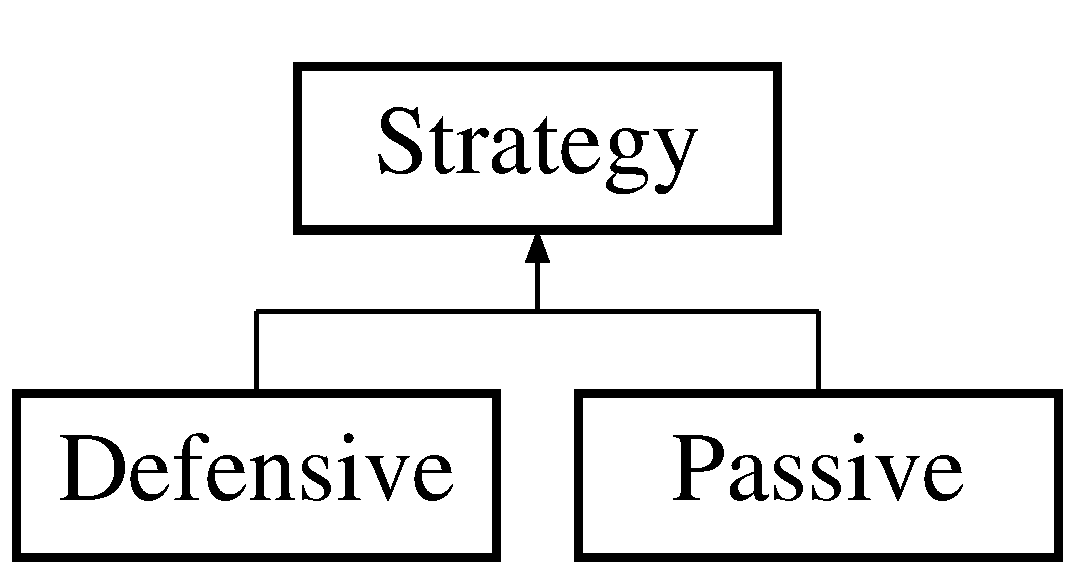
\includegraphics[height=2.000000cm]{classStrategy}
\end{center}
\end{figure}
\doxysubsection*{Public Member Functions}
\begin{DoxyCompactItemize}
\item 
<<<<<<< HEAD
\mbox{\Hypertarget{classStrategy_a2021a15bbc4f0d13f7b92f8933db2235}\label{classStrategy_a2021a15bbc4f0d13f7b92f8933db2235}} 
\hyperlink{classStrategy_a2021a15bbc4f0d13f7b92f8933db2235}{Strategy} ()
\begin{DoxyCompactList}\small\item\em Construct a new \hyperlink{classStrategy}{Strategy} object. \end{DoxyCompactList}\item 
\mbox{\Hypertarget{classStrategy_a37c0bbdd64fd7dfcdd91578784a64775}\label{classStrategy_a37c0bbdd64fd7dfcdd91578784a64775}} 
\hyperlink{classStrategy_a37c0bbdd64fd7dfcdd91578784a64775}{$\sim$\+Strategy} ()
\begin{DoxyCompactList}\small\item\em Destroy the \hyperlink{classStrategy}{Strategy} object. \end{DoxyCompactList}\item 
\mbox{\Hypertarget{classStrategy_aa0692005cb67d0ee2441046f6b302e7d}\label{classStrategy_aa0692005cb67d0ee2441046f6b302e7d}} 
virtual void {\bfseries perform\+Strat} (Key\+Point $\ast$key\+Point, Alliance $\ast$alliance)=0
\item 
virtual \hyperlink{classStrategy}{Strategy} $\ast$ \hyperlink{classStrategy_aaed20ba057db079ae2bc41b19b009211}{clone} ()=0
\begin{DoxyCompactList}\small\item\em Returns the cloned \hyperlink{classStrategy}{Strategy} object. \end{DoxyCompactList}\end{DoxyCompactItemize}
\subsection*{Protected Attributes}
=======
\mbox{\hyperlink{classStrategy_a2021a15bbc4f0d13f7b92f8933db2235}{Strategy}} ()
\begin{DoxyCompactList}\small\item\em Construct a new \mbox{\hyperlink{classStrategy}{Strategy}} object. \end{DoxyCompactList}\item 
\mbox{\hyperlink{classStrategy_a37c0bbdd64fd7dfcdd91578784a64775}{$\sim$\+Strategy}} ()
\begin{DoxyCompactList}\small\item\em Destroy the \mbox{\hyperlink{classStrategy}{Strategy}} object. \end{DoxyCompactList}\item 
virtual void \mbox{\hyperlink{classStrategy_aa0692005cb67d0ee2441046f6b302e7d}{perform\+Strat}} (\mbox{\hyperlink{classKeyPoint}{Key\+Point}} $\ast$key\+Point, \mbox{\hyperlink{classAlliance}{Alliance}} $\ast$alliance)=0
\item 
virtual \mbox{\hyperlink{classStrategy}{Strategy}} $\ast$ \mbox{\hyperlink{classStrategy_a552c2eba68a51d04aab5795508dcb075}{clone}} ()=0
\end{DoxyCompactItemize}
\doxysubsection*{Protected Attributes}
>>>>>>> 7be49738cebc0ced3357f2ce74f6fda2ea0b3d5e
\begin{DoxyCompactItemize}
\item 
std\+::string \mbox{\hyperlink{classStrategy_ab27bc814cf1804ca3b5fdbfb99d4a2cb}{strategy}}
\end{DoxyCompactItemize}


\doxysubsection{Detailed Description}


<<<<<<< HEAD
Definition at line 10 of file Strategy.\+h.



\subsection{Member Function Documentation}
\mbox{\Hypertarget{classStrategy_aaed20ba057db079ae2bc41b19b009211}\label{classStrategy_aaed20ba057db079ae2bc41b19b009211}} 
\index{Strategy@{Strategy}!clone@{clone}}
\index{clone@{clone}!Strategy@{Strategy}}
\subsubsection{\texorpdfstring{clone()}{clone()}}
{\footnotesize\ttfamily virtual \hyperlink{classStrategy}{Strategy}$\ast$ Strategy\+::clone (\begin{DoxyParamCaption}{ }\end{DoxyParamCaption})\hspace{0.3cm}{\ttfamily [pure virtual]}}



Returns the cloned \hyperlink{classStrategy}{Strategy} object. 

Post\+Conditions\+:
\begin{DoxyItemize}
\item Returns the clone of the current \hyperlink{classStrategy}{Strategy}
\end{DoxyItemize}

\begin{DoxyReturn}{Returns}
Strategy$\ast$ The cloned object 
\end{DoxyReturn}


Implemented in \hyperlink{classDefensive_afad21efc8bf51879f85f9d02e695cfa6}{Defensive}, and \hyperlink{classPassive_a576243ca77e794959cfcb33e772856a4}{Passive}.
=======
Definition at line \mbox{\hyperlink{Strategy_8h_source_l00010}{10}} of file \mbox{\hyperlink{Strategy_8h_source}{Strategy.\+h}}.



\doxysubsection{Constructor \& Destructor Documentation}
\mbox{\Hypertarget{classStrategy_a2021a15bbc4f0d13f7b92f8933db2235}\label{classStrategy_a2021a15bbc4f0d13f7b92f8933db2235}} 
\index{Strategy@{Strategy}!Strategy@{Strategy}}
\index{Strategy@{Strategy}!Strategy@{Strategy}}
\doxysubsubsection{\texorpdfstring{Strategy()}{Strategy()}}
{\footnotesize\ttfamily Strategy\+::\+Strategy (\begin{DoxyParamCaption}{ }\end{DoxyParamCaption})}



Construct a new \mbox{\hyperlink{classStrategy}{Strategy}} object. 



Definition at line \mbox{\hyperlink{Strategy_8cpp_source_l00007}{7}} of file \mbox{\hyperlink{Strategy_8cpp_source}{Strategy.\+cpp}}.


\begin{DoxyCode}{0}
\DoxyCodeLine{00007 \{\}}

\end{DoxyCode}
\mbox{\Hypertarget{classStrategy_a37c0bbdd64fd7dfcdd91578784a64775}\label{classStrategy_a37c0bbdd64fd7dfcdd91578784a64775}} 
\index{Strategy@{Strategy}!````~Strategy@{$\sim$Strategy}}
\index{````~Strategy@{$\sim$Strategy}!Strategy@{Strategy}}
\doxysubsubsection{\texorpdfstring{$\sim$Strategy()}{~Strategy()}}
{\footnotesize\ttfamily Strategy\+::$\sim$\+Strategy (\begin{DoxyParamCaption}{ }\end{DoxyParamCaption})}



Destroy the \mbox{\hyperlink{classStrategy}{Strategy}} object. 



Definition at line \mbox{\hyperlink{Strategy_8cpp_source_l00009}{9}} of file \mbox{\hyperlink{Strategy_8cpp_source}{Strategy.\+cpp}}.


\begin{DoxyCode}{0}
\DoxyCodeLine{00009 \{\}}

\end{DoxyCode}


\doxysubsection{Member Function Documentation}
\mbox{\Hypertarget{classStrategy_a552c2eba68a51d04aab5795508dcb075}\label{classStrategy_a552c2eba68a51d04aab5795508dcb075}} 
\index{Strategy@{Strategy}!clone@{clone}}
\index{clone@{clone}!Strategy@{Strategy}}
\doxysubsubsection{\texorpdfstring{clone()}{clone()}}
{\footnotesize\ttfamily virtual \mbox{\hyperlink{classStrategy}{Strategy}} $\ast$ Strategy\+::clone (\begin{DoxyParamCaption}{ }\end{DoxyParamCaption})\hspace{0.3cm}{\ttfamily [pure virtual]}}



Implemented in \mbox{\hyperlink{classAggressive_a43a336fbcafb3a36545dad09de1c2eea}{Aggressive}}, \mbox{\hyperlink{classDefensive_afad21efc8bf51879f85f9d02e695cfa6}{Defensive}}, and \mbox{\hyperlink{classPassive_a576243ca77e794959cfcb33e772856a4}{Passive}}.

\mbox{\Hypertarget{classStrategy_aa0692005cb67d0ee2441046f6b302e7d}\label{classStrategy_aa0692005cb67d0ee2441046f6b302e7d}} 
\index{Strategy@{Strategy}!performStrat@{performStrat}}
\index{performStrat@{performStrat}!Strategy@{Strategy}}
\doxysubsubsection{\texorpdfstring{performStrat()}{performStrat()}}
{\footnotesize\ttfamily virtual void Strategy\+::perform\+Strat (\begin{DoxyParamCaption}\item[{\mbox{\hyperlink{classKeyPoint}{Key\+Point}} $\ast$}]{key\+Point,  }\item[{\mbox{\hyperlink{classAlliance}{Alliance}} $\ast$}]{alliance }\end{DoxyParamCaption})\hspace{0.3cm}{\ttfamily [pure virtual]}}



Implemented in \mbox{\hyperlink{classAggressive_a84122a24be95be256f9992c21127b0d1}{Aggressive}}, \mbox{\hyperlink{classDefensive_a4cc4f2f71160bcade2cf2be8ade39903}{Defensive}}, and \mbox{\hyperlink{classPassive_ab296d4f8ba8ad68dacef1f80e3041aa7}{Passive}}.



\doxysubsection{Member Data Documentation}
\mbox{\Hypertarget{classStrategy_ab27bc814cf1804ca3b5fdbfb99d4a2cb}\label{classStrategy_ab27bc814cf1804ca3b5fdbfb99d4a2cb}} 
\index{Strategy@{Strategy}!strategy@{strategy}}
\index{strategy@{strategy}!Strategy@{Strategy}}
\doxysubsubsection{\texorpdfstring{strategy}{strategy}}
{\footnotesize\ttfamily std\+::string Strategy\+::strategy\hspace{0.3cm}{\ttfamily [protected]}}



Definition at line \mbox{\hyperlink{Strategy_8h_source_l00013}{13}} of file \mbox{\hyperlink{Strategy_8h_source}{Strategy.\+h}}.
>>>>>>> 7be49738cebc0ced3357f2ce74f6fda2ea0b3d5e



The documentation for this class was generated from the following files\+:\begin{DoxyCompactItemize}
\item 
Strategy.\+h\item 
Strategy.\+cpp\end{DoxyCompactItemize}

\hypertarget{classSunny}{}\doxysection{Sunny Class Reference}
\label{classSunny}\index{Sunny@{Sunny}}
Inheritance diagram for Sunny\+:\begin{figure}[H]
\begin{center}
\leavevmode
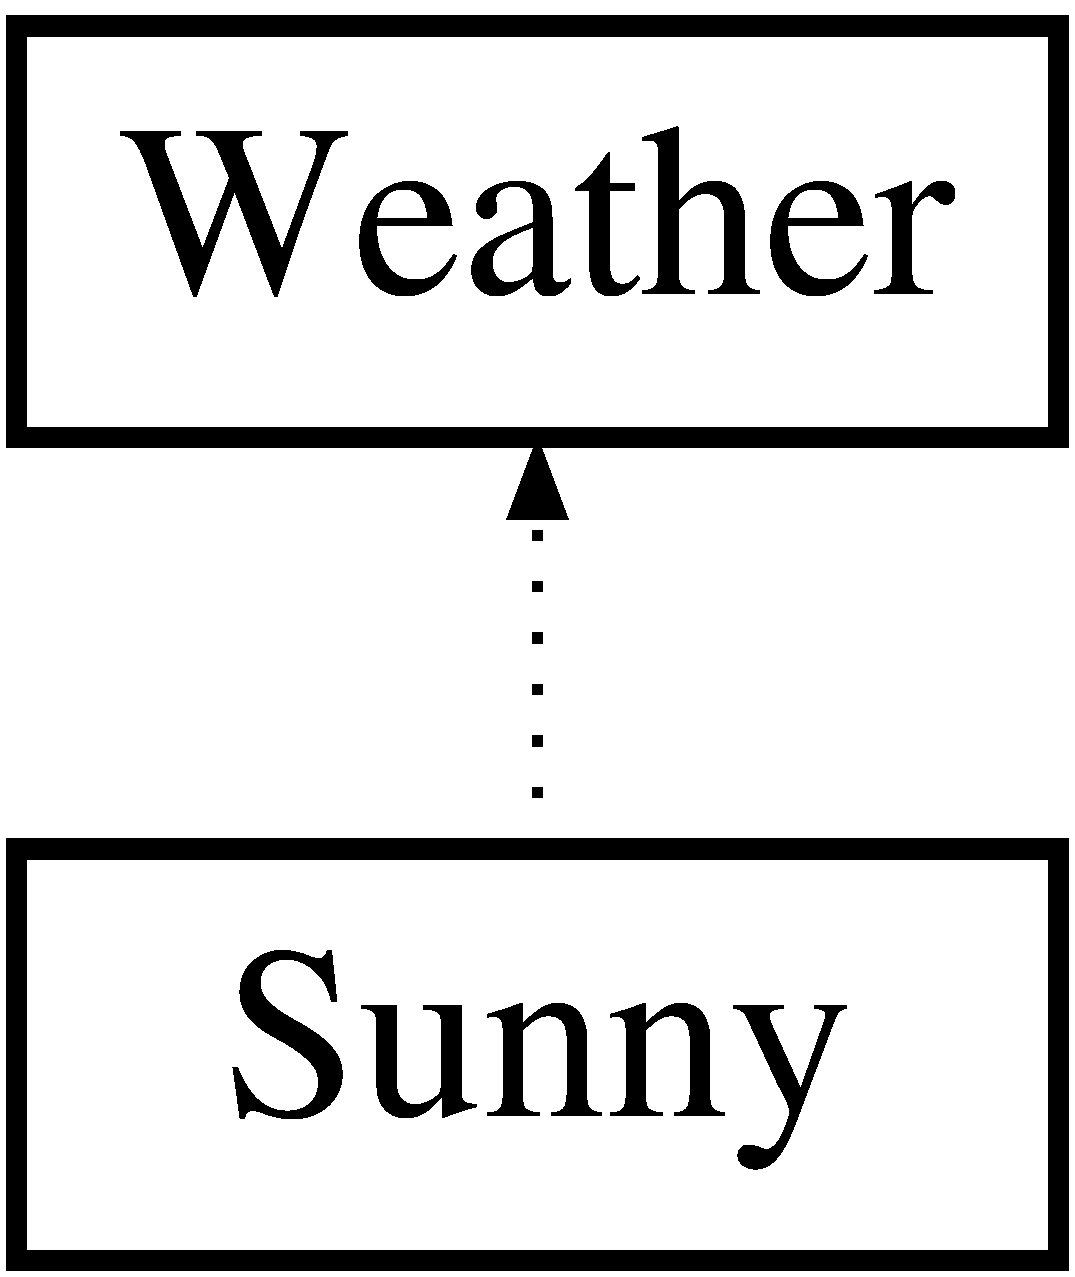
\includegraphics[height=2.000000cm]{classSunny}
\end{center}
\end{figure}
\doxysubsection*{Public Member Functions}
\begin{DoxyCompactItemize}
\item 
\mbox{\hyperlink{classSunny_a7f849e14ad8e3da056638135729f293d}{Sunny}} ()
\begin{DoxyCompactList}\small\item\em Instantiates the \mbox{\hyperlink{classSunny}{Sunny}} object of the state pattern. \end{DoxyCompactList}\item 
virtual std\+::string \mbox{\hyperlink{classSunny_a46747aed1564621c150127532b0d84f5}{get\+Weather}} ()
\begin{DoxyCompactList}\small\item\em Returns string which tells us the weather. \end{DoxyCompactList}\item 
virtual void \mbox{\hyperlink{classSunny_a940d045e5bfef4e92233f0269a194815}{handle\+Change}} (\mbox{\hyperlink{classKeyPoint}{Key\+Point}} $\ast$k)
\begin{DoxyCompactList}\small\item\em Will change the current state of the weather inside the specific keypoint. \end{DoxyCompactList}\end{DoxyCompactItemize}
\doxysubsection*{Additional Inherited Members}


\doxysubsection{Detailed Description}


Definition at line \mbox{\hyperlink{Sunny_8h_source_l00008}{8}} of file \mbox{\hyperlink{Sunny_8h_source}{Sunny.\+h}}.



\doxysubsection{Constructor \& Destructor Documentation}
\mbox{\Hypertarget{classSunny_a7f849e14ad8e3da056638135729f293d}\label{classSunny_a7f849e14ad8e3da056638135729f293d}} 
\index{Sunny@{Sunny}!Sunny@{Sunny}}
\index{Sunny@{Sunny}!Sunny@{Sunny}}
\doxysubsubsection{\texorpdfstring{Sunny()}{Sunny()}}
{\footnotesize\ttfamily Sunny\+::\+Sunny (\begin{DoxyParamCaption}{ }\end{DoxyParamCaption})}



Instantiates the \mbox{\hyperlink{classSunny}{Sunny}} object of the state pattern. 



Definition at line \mbox{\hyperlink{Sunny_8cpp_source_l00004}{4}} of file \mbox{\hyperlink{Sunny_8cpp_source}{Sunny.\+cpp}}.


\begin{DoxyCode}{0}
\DoxyCodeLine{00004              \{}
\DoxyCodeLine{00005     this-\/>multiplier = 1.0;}
\DoxyCodeLine{00006 \}}

\end{DoxyCode}


\doxysubsection{Member Function Documentation}
\mbox{\Hypertarget{classSunny_a46747aed1564621c150127532b0d84f5}\label{classSunny_a46747aed1564621c150127532b0d84f5}} 
\index{Sunny@{Sunny}!getWeather@{getWeather}}
\index{getWeather@{getWeather}!Sunny@{Sunny}}
\doxysubsubsection{\texorpdfstring{getWeather()}{getWeather()}}
{\footnotesize\ttfamily std\+::string Sunny\+::get\+Weather (\begin{DoxyParamCaption}{ }\end{DoxyParamCaption})\hspace{0.3cm}{\ttfamily [virtual]}}



Returns string which tells us the weather. 

Postconditions\+:
\begin{DoxyItemize}
\item Returns the wether of ths current state
\end{DoxyItemize}

\begin{DoxyReturn}{Returns}
std\+::string which is the current state 
\end{DoxyReturn}


Implements \mbox{\hyperlink{classWeather}{Weather}}.



Definition at line \mbox{\hyperlink{Sunny_8cpp_source_l00008}{8}} of file \mbox{\hyperlink{Sunny_8cpp_source}{Sunny.\+cpp}}.


\begin{DoxyCode}{0}
\DoxyCodeLine{00008                             \{}
\DoxyCodeLine{00009     \textcolor{keywordflow}{return} \textcolor{stringliteral}{"{}Sunny"{}};}
\DoxyCodeLine{00010 \}}

\end{DoxyCode}
\mbox{\Hypertarget{classSunny_a940d045e5bfef4e92233f0269a194815}\label{classSunny_a940d045e5bfef4e92233f0269a194815}} 
\index{Sunny@{Sunny}!handleChange@{handleChange}}
\index{handleChange@{handleChange}!Sunny@{Sunny}}
\doxysubsubsection{\texorpdfstring{handleChange()}{handleChange()}}
{\footnotesize\ttfamily void Sunny\+::handle\+Change (\begin{DoxyParamCaption}\item[{\mbox{\hyperlink{classKeyPoint}{Key\+Point}} $\ast$}]{k }\end{DoxyParamCaption})\hspace{0.3cm}{\ttfamily [virtual]}}



Will change the current state of the weather inside the specific keypoint. 

Preconditions\+:
\begin{DoxyItemize}
\item k must be a Key\+Point$\ast$
\end{DoxyItemize}

Postconditions\+:
\begin{DoxyItemize}
\item Changes the current weather to the next one in the state pattern (\mbox{\hyperlink{classCloudy}{Cloudy}})
\end{DoxyItemize}


\begin{DoxyParams}{Parameters}
{\em k} & must be a Key\+Point$\ast$ \\
\hline
\end{DoxyParams}
\begin{DoxyReturn}{Returns}
void 
\end{DoxyReturn}


Implements \mbox{\hyperlink{classWeather}{Weather}}.



Definition at line \mbox{\hyperlink{Sunny_8cpp_source_l00012}{12}} of file \mbox{\hyperlink{Sunny_8cpp_source}{Sunny.\+cpp}}.


\begin{DoxyCode}{0}
\DoxyCodeLine{00012                                     \{}
\DoxyCodeLine{00013     \mbox{\hyperlink{classCloudy}{Cloudy}}* newWeather = \textcolor{keyword}{new} \mbox{\hyperlink{classCloudy}{Cloudy}}();}
\DoxyCodeLine{00014     k-\/>\mbox{\hyperlink{classKeyPoint_a5c4b9314440a00fca7ab4d82ea4693a5}{setWeather}}(newWeather);}
\DoxyCodeLine{00015 \}}

\end{DoxyCode}


The documentation for this class was generated from the following files\+:\begin{DoxyCompactItemize}
\item 
Sunny.\+h\item 
Sunny.\+cpp\end{DoxyCompactItemize}

\hypertarget{classSupport}{}\doxysection{Support Class Reference}
\label{classSupport}\index{Support@{Support}}


\mbox{\hyperlink{classSupport}{Support}} class.  




{\ttfamily \#include $<$Support.\+h$>$}

Inheritance diagram for Support\+:\begin{figure}[H]
\begin{center}
\leavevmode
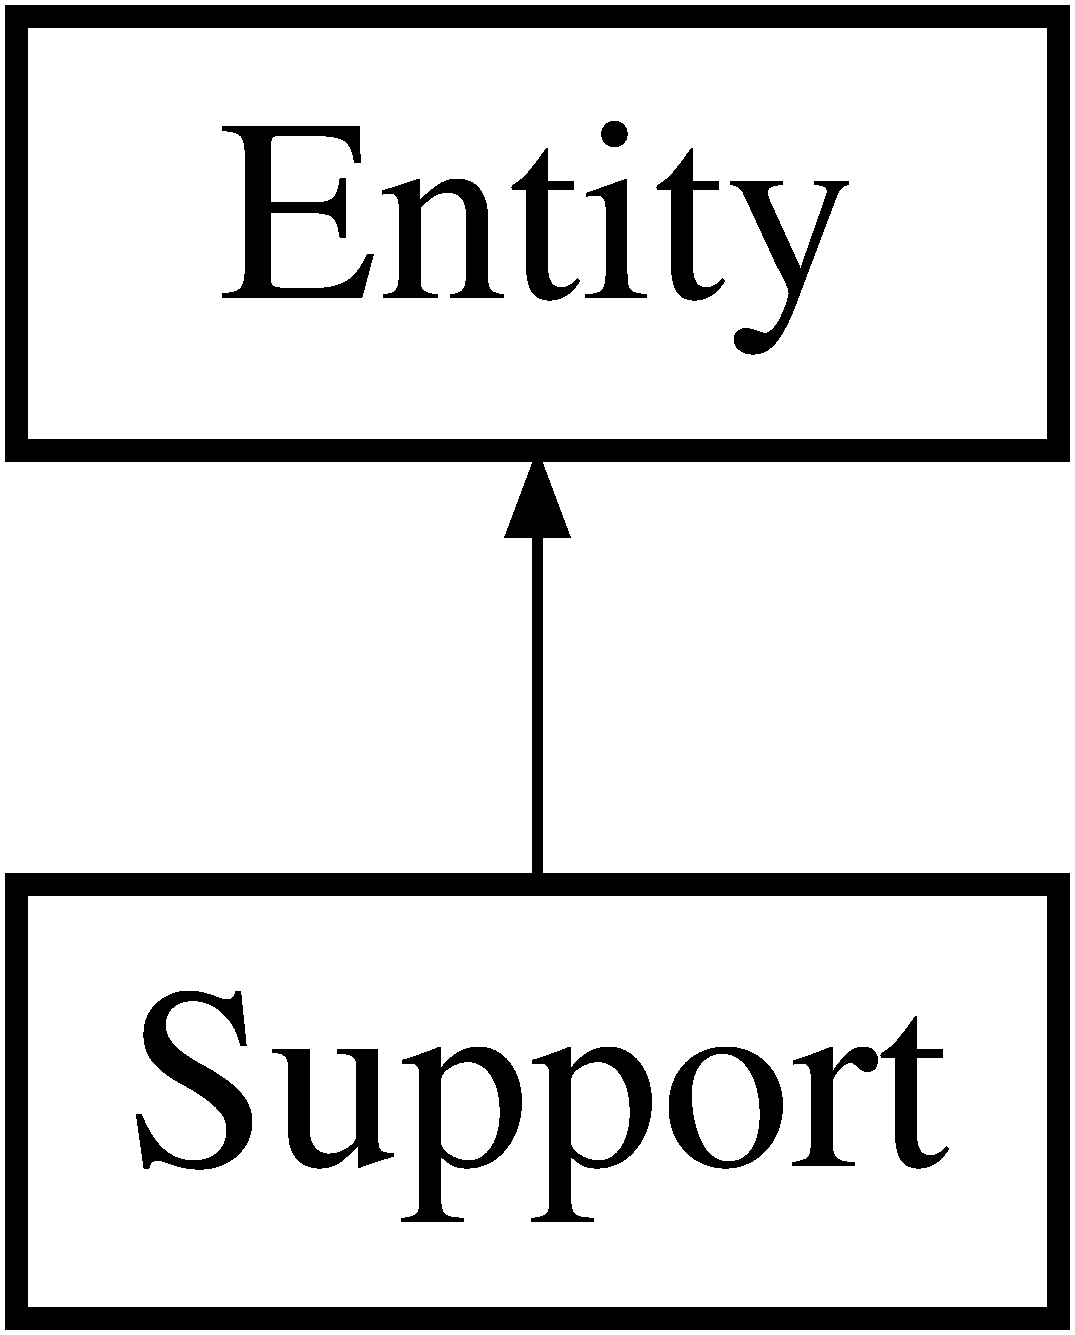
\includegraphics[height=2.000000cm]{classSupport}
\end{center}
\end{figure}
\doxysubsection*{Public Member Functions}
\begin{DoxyCompactItemize}
\item 
\mbox{\hyperlink{classSupport_a8b4c631dcfd81be50ee86f3ed01d5c1e}{Support}} (\mbox{\hyperlink{classType}{Type}} $\ast$type, int health=1000, int damage=30)
\begin{DoxyCompactList}\small\item\em Instantiates the support. \end{DoxyCompactList}\item 
void \mbox{\hyperlink{classSupport_afb159bd8c474ec67ad5d03fa24c38564}{take\+Damage}} (int damage)
\begin{DoxyCompactList}\small\item\em Removes health from the support object. \end{DoxyCompactList}\item 
void \mbox{\hyperlink{classSupport_a5f2cb243e746adea36b3c78548029ce3}{deal\+Damage}} (\mbox{\hyperlink{classEntity}{Entity}} $\ast$entity)
\begin{DoxyCompactList}\small\item\em Inflicts damage onto another entity. \end{DoxyCompactList}\end{DoxyCompactItemize}


\doxysubsection{Detailed Description}
\mbox{\hyperlink{classSupport}{Support}} class. 

Used to add addtional functionality to \mbox{\hyperlink{classEntity}{Entity}} objects. 

Definition at line \mbox{\hyperlink{Support_8h_source_l00011}{11}} of file \mbox{\hyperlink{Support_8h_source}{Support.\+h}}.



\doxysubsection{Constructor \& Destructor Documentation}
\mbox{\Hypertarget{classSupport_a8b4c631dcfd81be50ee86f3ed01d5c1e}\label{classSupport_a8b4c631dcfd81be50ee86f3ed01d5c1e}} 
\index{Support@{Support}!Support@{Support}}
\index{Support@{Support}!Support@{Support}}
\doxysubsubsection{\texorpdfstring{Support()}{Support()}}
{\footnotesize\ttfamily Support\+::\+Support (\begin{DoxyParamCaption}\item[{\mbox{\hyperlink{classType}{Type}} $\ast$}]{type,  }\item[{int}]{health = {\ttfamily 1000},  }\item[{int}]{damage = {\ttfamily 30} }\end{DoxyParamCaption})}



Instantiates the support. 


\begin{DoxyParams}{Parameters}
{\em health} & must be an int \\
\hline
{\em damage} & must be an int \\
\hline
{\em type} & must be a Type$\ast$ \\
\hline
\end{DoxyParams}


Definition at line \mbox{\hyperlink{Support_8cpp_source_l00003}{3}} of file \mbox{\hyperlink{Support_8cpp_source}{Support.\+cpp}}.


\begin{DoxyCode}{0}
\DoxyCodeLine{00003 : \mbox{\hyperlink{classEntity}{Entity}}(type, health, damage) \{\}}

\end{DoxyCode}


\doxysubsection{Member Function Documentation}
\mbox{\Hypertarget{classSupport_a5f2cb243e746adea36b3c78548029ce3}\label{classSupport_a5f2cb243e746adea36b3c78548029ce3}} 
\index{Support@{Support}!dealDamage@{dealDamage}}
\index{dealDamage@{dealDamage}!Support@{Support}}
\doxysubsubsection{\texorpdfstring{dealDamage()}{dealDamage()}}
{\footnotesize\ttfamily void Support\+::deal\+Damage (\begin{DoxyParamCaption}\item[{\mbox{\hyperlink{classEntity}{Entity}} $\ast$}]{entity }\end{DoxyParamCaption})\hspace{0.3cm}{\ttfamily [virtual]}}



Inflicts damage onto another entity. 

Preconditions\+:
\begin{DoxyItemize}
\item entity must be an Entity$\ast$
\end{DoxyItemize}

Postconditions\+:
\begin{DoxyItemize}
\item Reduces the health of the entity
\end{DoxyItemize}


\begin{DoxyParams}{Parameters}
{\em entity} & must be an Entity$\ast$ \\
\hline
\end{DoxyParams}
\begin{DoxyReturn}{Returns}
void 
\end{DoxyReturn}


Implements \mbox{\hyperlink{classEntity}{Entity}}.



Definition at line \mbox{\hyperlink{Support_8cpp_source_l00005}{5}} of file \mbox{\hyperlink{Support_8cpp_source}{Support.\+cpp}}.


\begin{DoxyCode}{0}
\DoxyCodeLine{00005                                        \{}
\DoxyCodeLine{00006     entity-\/>takeDamage(\mbox{\hyperlink{classEntity_ad38d4384aa0adef43443666a33f06508}{getDamage}}());}
\DoxyCodeLine{00007 \}}

\end{DoxyCode}
\mbox{\Hypertarget{classSupport_afb159bd8c474ec67ad5d03fa24c38564}\label{classSupport_afb159bd8c474ec67ad5d03fa24c38564}} 
\index{Support@{Support}!takeDamage@{takeDamage}}
\index{takeDamage@{takeDamage}!Support@{Support}}
\doxysubsubsection{\texorpdfstring{takeDamage()}{takeDamage()}}
{\footnotesize\ttfamily void Support\+::take\+Damage (\begin{DoxyParamCaption}\item[{int}]{damage }\end{DoxyParamCaption})\hspace{0.3cm}{\ttfamily [virtual]}}



Removes health from the support object. 

Preconditions\+:
\begin{DoxyItemize}
\item damage must be an int
\end{DoxyItemize}

Postconditions\+:
\begin{DoxyItemize}
\item Reduces the health of the support object
\end{DoxyItemize}


\begin{DoxyParams}{Parameters}
{\em damage} & must be an int \\
\hline
\end{DoxyParams}
\begin{DoxyReturn}{Returns}
void 
\end{DoxyReturn}


Implements \mbox{\hyperlink{classEntity}{Entity}}.



Definition at line \mbox{\hyperlink{Support_8cpp_source_l00009}{9}} of file \mbox{\hyperlink{Support_8cpp_source}{Support.\+cpp}}.


\begin{DoxyCode}{0}
\DoxyCodeLine{00009                                    \{}
\DoxyCodeLine{00010     this-\/>\mbox{\hyperlink{classEntity_a7dae281ff92be9bc98672cafe05c77ab}{setHealth}}(this-\/>\mbox{\hyperlink{classEntity_a2b0140ae8c77c0e3654b070ee3c7fe57}{getHealth}}() -\/ damage);}
\DoxyCodeLine{00011 \}}

\end{DoxyCode}


The documentation for this class was generated from the following files\+:\begin{DoxyCompactItemize}
\item 
Support.\+h\item 
Support.\+cpp\end{DoxyCompactItemize}

\hypertarget{classSupportFactory}{}\doxysection{Support\+Factory Class Reference}
\label{classSupportFactory}\index{SupportFactory@{SupportFactory}}


\mbox{\hyperlink{classSupportFactory}{Support\+Factory}} class.  




{\ttfamily \#include $<$Support\+Factory.\+h$>$}

Inheritance diagram for Support\+Factory\+:\begin{figure}[H]
\begin{center}
\leavevmode
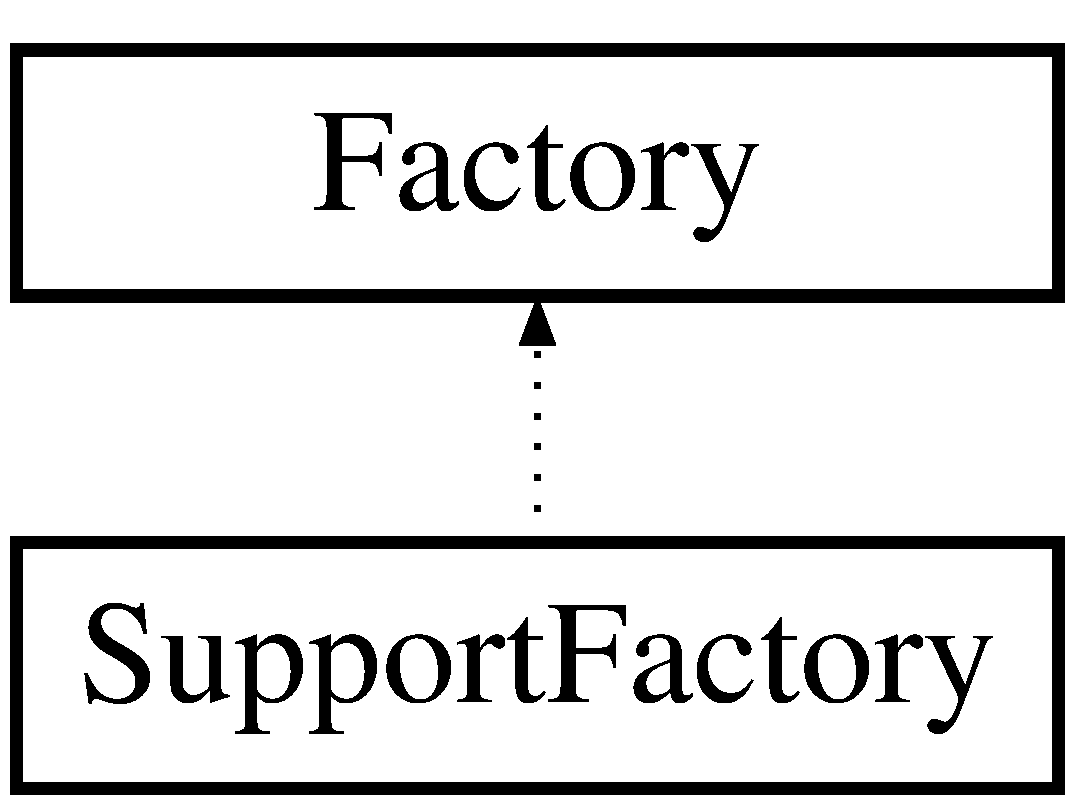
\includegraphics[height=2.000000cm]{classSupportFactory}
\end{center}
\end{figure}
\doxysubsection*{Public Member Functions}
\begin{DoxyCompactItemize}
\item 
\mbox{\hyperlink{classSupportFactory_a8e0b10fb625f7d4a93cec9989bef45c4}{Support\+Factory}} (\mbox{\hyperlink{classType}{Type}} $\ast$type, \mbox{\hyperlink{classAddOn}{Add\+On}} $\ast$add\+On)
\begin{DoxyCompactList}\small\item\em Instantiates the support factory. \end{DoxyCompactList}\item 
\mbox{\hyperlink{classEntity}{Entity}} $\ast$ \mbox{\hyperlink{classSupportFactory_ad2ebc8fdf1335e423a766fa0c5573cf8}{create\+Entity}} (\mbox{\hyperlink{classAlliance}{Alliance}} $\ast$alliance)
\begin{DoxyCompactList}\small\item\em Instantiates and returns a support for the given alliance. \end{DoxyCompactList}\item 
\mbox{\hyperlink{classFactory}{Factory}} $\ast$ \mbox{\hyperlink{classSupportFactory_a802c25e901b479656ea95a5678a1ad26}{clone}} ()
\begin{DoxyCompactList}\small\item\em Instantiates and returns a clone of the current support factory. \end{DoxyCompactList}\end{DoxyCompactItemize}


\doxysubsection{Detailed Description}
\mbox{\hyperlink{classSupportFactory}{Support\+Factory}} class. 

Used to instantiate \mbox{\hyperlink{classSupport}{Support}} objects. 

Definition at line \mbox{\hyperlink{SupportFactory_8h_source_l00011}{11}} of file \mbox{\hyperlink{SupportFactory_8h_source}{Support\+Factory.\+h}}.



\doxysubsection{Constructor \& Destructor Documentation}
\mbox{\Hypertarget{classSupportFactory_a8e0b10fb625f7d4a93cec9989bef45c4}\label{classSupportFactory_a8e0b10fb625f7d4a93cec9989bef45c4}} 
\index{SupportFactory@{SupportFactory}!SupportFactory@{SupportFactory}}
\index{SupportFactory@{SupportFactory}!SupportFactory@{SupportFactory}}
\doxysubsubsection{\texorpdfstring{SupportFactory()}{SupportFactory()}}
{\footnotesize\ttfamily Support\+Factory\+::\+Support\+Factory (\begin{DoxyParamCaption}\item[{\mbox{\hyperlink{classType}{Type}} $\ast$}]{type,  }\item[{\mbox{\hyperlink{classAddOn}{Add\+On}} $\ast$}]{add\+On }\end{DoxyParamCaption})}



Instantiates the support factory. 


\begin{DoxyParams}{Parameters}
{\em type} & must be a Type$\ast$ \\
\hline
{\em add\+On} & must be a Add\+On$\ast$ \\
\hline
\end{DoxyParams}


Definition at line \mbox{\hyperlink{SupportFactory_8cpp_source_l00004}{4}} of file \mbox{\hyperlink{SupportFactory_8cpp_source}{Support\+Factory.\+cpp}}.


\begin{DoxyCode}{0}
\DoxyCodeLine{00004 : \mbox{\hyperlink{classFactory}{Factory}}(type, addOn) \{\}}

\end{DoxyCode}


\doxysubsection{Member Function Documentation}
\mbox{\Hypertarget{classSupportFactory_a802c25e901b479656ea95a5678a1ad26}\label{classSupportFactory_a802c25e901b479656ea95a5678a1ad26}} 
\index{SupportFactory@{SupportFactory}!clone@{clone}}
\index{clone@{clone}!SupportFactory@{SupportFactory}}
\doxysubsubsection{\texorpdfstring{clone()}{clone()}}
{\footnotesize\ttfamily \mbox{\hyperlink{classFactory}{Factory}} $\ast$ Support\+Factory\+::clone (\begin{DoxyParamCaption}{ }\end{DoxyParamCaption})\hspace{0.3cm}{\ttfamily [virtual]}}



Instantiates and returns a clone of the current support factory. 

Postconditions\+:
\begin{DoxyItemize}
\item Returns the clone of the current support factory
\end{DoxyItemize}

\begin{DoxyReturn}{Returns}
Factory$\ast$ The support factory clone 
\end{DoxyReturn}


Implements \mbox{\hyperlink{classFactory}{Factory}}.



Definition at line \mbox{\hyperlink{SupportFactory_8cpp_source_l00018}{18}} of file \mbox{\hyperlink{SupportFactory_8cpp_source}{Support\+Factory.\+cpp}}.


\begin{DoxyCode}{0}
\DoxyCodeLine{00018                                \{}
\DoxyCodeLine{00019     \textcolor{keywordflow}{return} \textcolor{keyword}{new} \mbox{\hyperlink{classSupportFactory}{SupportFactory}}(\mbox{\hyperlink{classFactory_ac91051006ace7ec5bb6ecf0fe6d02d58}{getType}}()-\/>\mbox{\hyperlink{classSupportFactory_a802c25e901b479656ea95a5678a1ad26}{clone}}(), \mbox{\hyperlink{classFactory_a994153930f59cafb280e91d5b100b5aa}{getAddOn}}()-\/>\mbox{\hyperlink{classSupportFactory_a802c25e901b479656ea95a5678a1ad26}{clone}}());}
\DoxyCodeLine{00020 \}}

\end{DoxyCode}
\mbox{\Hypertarget{classSupportFactory_ad2ebc8fdf1335e423a766fa0c5573cf8}\label{classSupportFactory_ad2ebc8fdf1335e423a766fa0c5573cf8}} 
\index{SupportFactory@{SupportFactory}!createEntity@{createEntity}}
\index{createEntity@{createEntity}!SupportFactory@{SupportFactory}}
\doxysubsubsection{\texorpdfstring{createEntity()}{createEntity()}}
{\footnotesize\ttfamily \mbox{\hyperlink{classEntity}{Entity}} $\ast$ Support\+Factory\+::create\+Entity (\begin{DoxyParamCaption}\item[{\mbox{\hyperlink{classAlliance}{Alliance}} $\ast$}]{alliance }\end{DoxyParamCaption})\hspace{0.3cm}{\ttfamily [virtual]}}



Instantiates and returns a support for the given alliance. 

Preconditions\+:
\begin{DoxyItemize}
\item alliance must be an Alliance$\ast$
\end{DoxyItemize}

Postconditions\+:
\begin{DoxyItemize}
\item Returns the instantiated support object with specific state
\end{DoxyItemize}


\begin{DoxyParams}{Parameters}
{\em alliance} & must be a Alliance$\ast$ \\
\hline
\end{DoxyParams}
\begin{DoxyReturn}{Returns}
Entity$\ast$ The instatiated support 
\end{DoxyReturn}


Implements \mbox{\hyperlink{classFactory}{Factory}}.



Definition at line \mbox{\hyperlink{SupportFactory_8cpp_source_l00006}{6}} of file \mbox{\hyperlink{SupportFactory_8cpp_source}{Support\+Factory.\+cpp}}.


\begin{DoxyCode}{0}
\DoxyCodeLine{00006                                                        \{}
\DoxyCodeLine{00007     \mbox{\hyperlink{classSupport}{Support}}* s = \textcolor{keyword}{new} \mbox{\hyperlink{classSupport}{Support}}(\mbox{\hyperlink{classFactory_ac91051006ace7ec5bb6ecf0fe6d02d58}{getType}}()-\/>\mbox{\hyperlink{classSupportFactory_a802c25e901b479656ea95a5678a1ad26}{clone}}());}
\DoxyCodeLine{00008     s-\/>\mbox{\hyperlink{classEntity_af804dcaa600e770cf0e2b4537f6fba23}{setAlliance}}(alliance);}
\DoxyCodeLine{00009     \textcolor{keywordflow}{if} (\mbox{\hyperlink{classFactory_a994153930f59cafb280e91d5b100b5aa}{getAddOn}}() != NULL) \{}
\DoxyCodeLine{00010         \mbox{\hyperlink{classAddOn}{AddOn}}* personnelAddOn = \mbox{\hyperlink{classFactory_a994153930f59cafb280e91d5b100b5aa}{getAddOn}}()-\/>clone();}
\DoxyCodeLine{00011         personnelAddOn-\/>\mbox{\hyperlink{classAddOn_ac9f4263e3558015fdad46adefceed197}{setEntity}}(s);}
\DoxyCodeLine{00012         \textcolor{keywordflow}{return} personnelAddOn;}
\DoxyCodeLine{00013     \} \textcolor{keywordflow}{else} \{}
\DoxyCodeLine{00014         \textcolor{keywordflow}{return} s;}
\DoxyCodeLine{00015     \}}
\DoxyCodeLine{00016 \}}

\end{DoxyCode}


The documentation for this class was generated from the following files\+:\begin{DoxyCompactItemize}
\item 
Support\+Factory.\+h\item 
Support\+Factory.\+cpp\end{DoxyCompactItemize}

\hypertarget{classTerrainType}{}\section{Terrain\+Type Class Reference}
\label{classTerrainType}\index{Terrain\+Type@{Terrain\+Type}}


\hyperlink{classTerrainType}{Terrain\+Type} class.  




{\ttfamily \#include $<$Terrain\+Type.\+h$>$}

Inheritance diagram for Terrain\+Type\+:\begin{figure}[H]
\begin{center}
\leavevmode
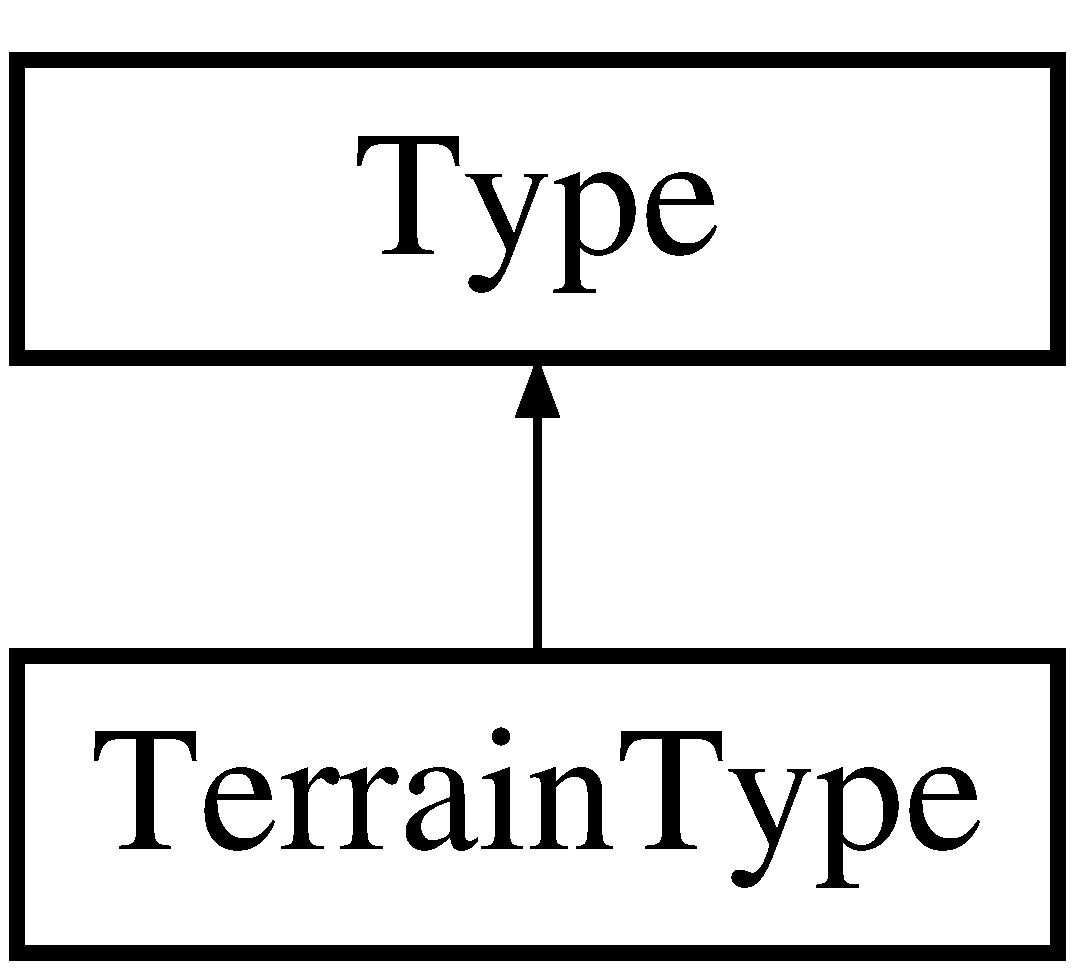
\includegraphics[height=2.000000cm]{classTerrainType}
\end{center}
\end{figure}
\subsection*{Public Member Functions}
\begin{DoxyCompactItemize}
\item 
\mbox{\Hypertarget{classTerrainType_aea114fb5e125b58bf9d9c9ab964749c7}\label{classTerrainType_aea114fb5e125b58bf9d9c9ab964749c7}} 
\hyperlink{classTerrainType_aea114fb5e125b58bf9d9c9ab964749c7}{Terrain\+Type} ()
\begin{DoxyCompactList}\small\item\em Instantiates the terrain type. \end{DoxyCompactList}\item 
string \hyperlink{classTerrainType_af24f4291676b6862c90b0d29598fcb11}{get\+Type\+Desc} ()
\begin{DoxyCompactList}\small\item\em Returns terrain type description. \end{DoxyCompactList}\item 
\hyperlink{classType}{Type} $\ast$ \hyperlink{classTerrainType_aa2c54fdc07981dab3941f28221e22655}{clone} ()
\begin{DoxyCompactList}\small\item\em returns the the cloned object of \hyperlink{classType}{Type} \end{DoxyCompactList}\end{DoxyCompactItemize}


\subsection{Detailed Description}
\hyperlink{classTerrainType}{Terrain\+Type} class. 

Used to define Entity objects as terrain type. 

Definition at line 11 of file Terrain\+Type.\+h.



\subsection{Member Function Documentation}
\mbox{\Hypertarget{classTerrainType_aa2c54fdc07981dab3941f28221e22655}\label{classTerrainType_aa2c54fdc07981dab3941f28221e22655}} 
\index{Terrain\+Type@{Terrain\+Type}!clone@{clone}}
\index{clone@{clone}!Terrain\+Type@{Terrain\+Type}}
\subsubsection{\texorpdfstring{clone()}{clone()}}
{\footnotesize\ttfamily \hyperlink{classType}{Type} $\ast$ Terrain\+Type\+::clone (\begin{DoxyParamCaption}{ }\end{DoxyParamCaption})\hspace{0.3cm}{\ttfamily [virtual]}}



returns the the cloned object of \hyperlink{classType}{Type} 

Post\+Conditions\+:
\begin{DoxyItemize}
\item returns Type$\ast$ type
\end{DoxyItemize}

\begin{DoxyReturn}{Returns}
Type$\ast$ The cloned \hyperlink{classType}{Type} object 
\end{DoxyReturn}


Implements \hyperlink{classType_a7b79d264e2cbac9c091cdb41ffb112c9}{Type}.



Definition at line 9 of file Terrain\+Type.\+cpp.


\begin{DoxyCode}
9                          \{
10     \textcolor{keywordflow}{return} \textcolor{keyword}{new} \hyperlink{classTerrainType_aea114fb5e125b58bf9d9c9ab964749c7}{TerrainType}();
11 \}
\end{DoxyCode}
\mbox{\Hypertarget{classTerrainType_af24f4291676b6862c90b0d29598fcb11}\label{classTerrainType_af24f4291676b6862c90b0d29598fcb11}} 
\index{Terrain\+Type@{Terrain\+Type}!get\+Type\+Desc@{get\+Type\+Desc}}
\index{get\+Type\+Desc@{get\+Type\+Desc}!Terrain\+Type@{Terrain\+Type}}
\subsubsection{\texorpdfstring{get\+Type\+Desc()}{getTypeDesc()}}
{\footnotesize\ttfamily string Terrain\+Type\+::get\+Type\+Desc (\begin{DoxyParamCaption}{ }\end{DoxyParamCaption})\hspace{0.3cm}{\ttfamily [virtual]}}



Returns terrain type description. 

Postconditions\+:
\begin{DoxyItemize}
\item Returns the terrain type
\end{DoxyItemize}

\begin{DoxyReturn}{Returns}
string The terrain type string 
\end{DoxyReturn}


Implements \hyperlink{classType_a5c453300dc060252c30534110bd2f78c}{Type}.



Definition at line 5 of file Terrain\+Type.\+cpp.


\begin{DoxyCode}
5                                 \{
6     \textcolor{keywordflow}{return} \textcolor{stringliteral}{"Terrain"};
7 \}
\end{DoxyCode}


The documentation for this class was generated from the following files\+:\begin{DoxyCompactItemize}
\item 
Terrain\+Type.\+h\item 
Terrain\+Type.\+cpp\end{DoxyCompactItemize}

\hypertarget{classType}{}\section{Type Class Reference}
\label{classType}\index{Type@{Type}}


\hyperlink{classType}{Type} class.  




{\ttfamily \#include $<$Type.\+h$>$}

Inheritance diagram for Type\+:\begin{figure}[H]
\begin{center}
\leavevmode
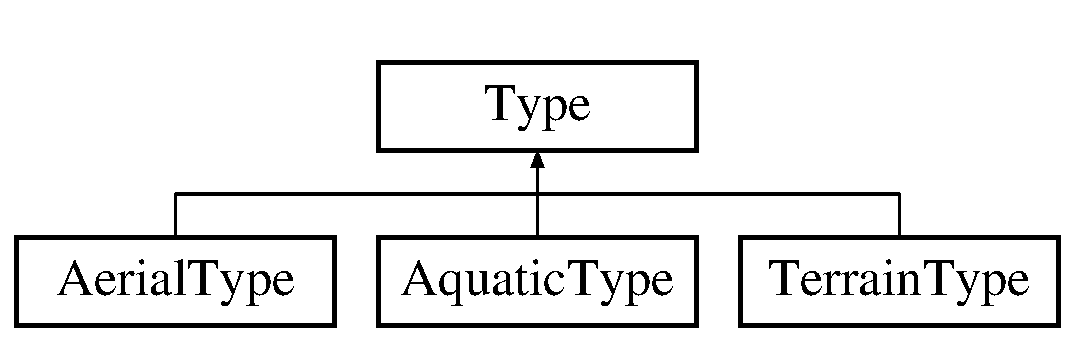
\includegraphics[height=2.000000cm]{classType}
\end{center}
\end{figure}
\subsection*{Public Member Functions}
\begin{DoxyCompactItemize}
\item 
\mbox{\Hypertarget{classType_a78339313d36891f18427c431ea84e306}\label{classType_a78339313d36891f18427c431ea84e306}} 
\hyperlink{classType_a78339313d36891f18427c431ea84e306}{Type} ()
\begin{DoxyCompactList}\small\item\em Instantiates the type. \end{DoxyCompactList}\item 
virtual string \hyperlink{classType_a5c453300dc060252c30534110bd2f78c}{get\+Type\+Desc} ()=0
\begin{DoxyCompactList}\small\item\em Returns terrain type description. \end{DoxyCompactList}\item 
virtual \hyperlink{classType}{Type} $\ast$ \hyperlink{classType_a7b79d264e2cbac9c091cdb41ffb112c9}{clone} ()=0
\begin{DoxyCompactList}\small\item\em returns the the cloned object of \hyperlink{classType}{Type} \end{DoxyCompactList}\end{DoxyCompactItemize}


\subsection{Detailed Description}
\hyperlink{classType}{Type} class. 

Used to define Entity objects type. 

Definition at line 13 of file Type.\+h.



\subsection{Member Function Documentation}
\mbox{\Hypertarget{classType_a7b79d264e2cbac9c091cdb41ffb112c9}\label{classType_a7b79d264e2cbac9c091cdb41ffb112c9}} 
\index{Type@{Type}!clone@{clone}}
\index{clone@{clone}!Type@{Type}}
\subsubsection{\texorpdfstring{clone()}{clone()}}
{\footnotesize\ttfamily virtual \hyperlink{classType}{Type}$\ast$ Type\+::clone (\begin{DoxyParamCaption}{ }\end{DoxyParamCaption})\hspace{0.3cm}{\ttfamily [pure virtual]}}



returns the the cloned object of \hyperlink{classType}{Type} 

Post\+Conditions\+:
\begin{DoxyItemize}
\item returns Type$\ast$ type
\end{DoxyItemize}

\begin{DoxyReturn}{Returns}
Type$\ast$ The cloned \hyperlink{classType}{Type} object 
\end{DoxyReturn}


Implemented in \hyperlink{classAerialType_a8e7184b0b9e184142144df65f3da7fb1}{Aerial\+Type}, \hyperlink{classAquaticType_afbcc6f679b6108c7ed286ab0aa91bdd5}{Aquatic\+Type}, and \hyperlink{classTerrainType_aa2c54fdc07981dab3941f28221e22655}{Terrain\+Type}.

\mbox{\Hypertarget{classType_a5c453300dc060252c30534110bd2f78c}\label{classType_a5c453300dc060252c30534110bd2f78c}} 
\index{Type@{Type}!get\+Type\+Desc@{get\+Type\+Desc}}
\index{get\+Type\+Desc@{get\+Type\+Desc}!Type@{Type}}
\subsubsection{\texorpdfstring{get\+Type\+Desc()}{getTypeDesc()}}
{\footnotesize\ttfamily virtual string Type\+::get\+Type\+Desc (\begin{DoxyParamCaption}{ }\end{DoxyParamCaption})\hspace{0.3cm}{\ttfamily [pure virtual]}}



Returns terrain type description. 

Postconditions\+:
\begin{DoxyItemize}
\item Returns the terrain type
\end{DoxyItemize}

\begin{DoxyReturn}{Returns}
string The terrain type string 
\end{DoxyReturn}


Implemented in \hyperlink{classAerialType_a66dd43f2688de9a5eab9c6de0396e9cc}{Aerial\+Type}, \hyperlink{classAquaticType_abb1b9ebdb96a352e0287f7a7cb803eab}{Aquatic\+Type}, and \hyperlink{classTerrainType_af24f4291676b6862c90b0d29598fcb11}{Terrain\+Type}.



The documentation for this class was generated from the following files\+:\begin{DoxyCompactItemize}
\item 
Type.\+h\item 
Type.\+cpp\end{DoxyCompactItemize}

\hypertarget{classVehicle}{}\doxysection{Vehicle Class Reference}
\label{classVehicle}\index{Vehicle@{Vehicle}}
Inheritance diagram for Vehicle\+:\begin{figure}[H]
\begin{center}
\leavevmode
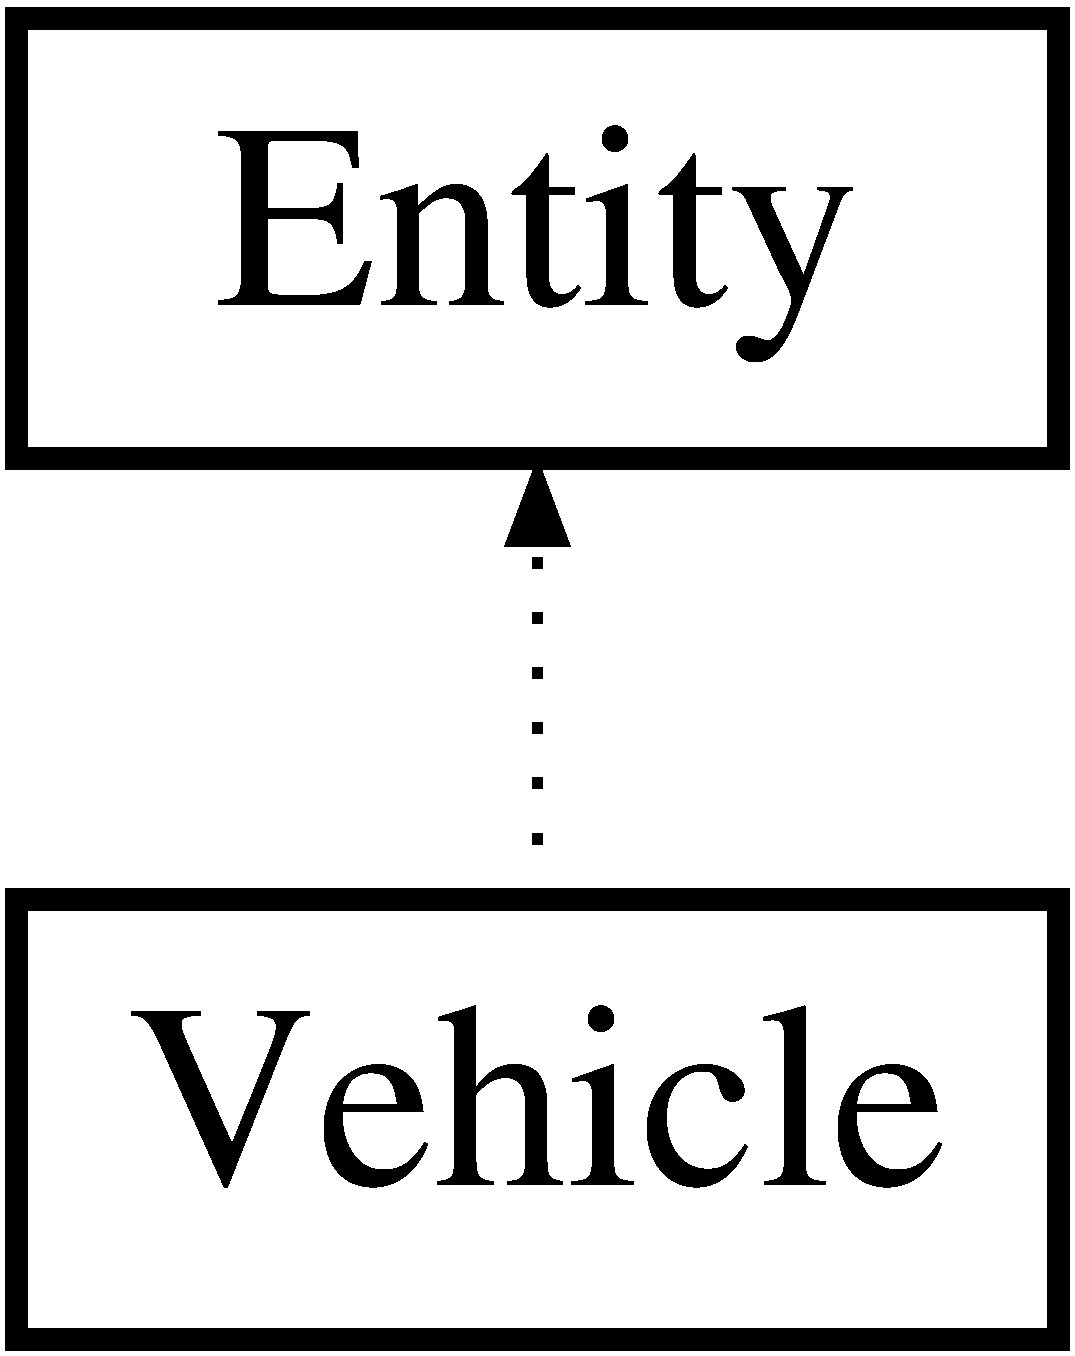
\includegraphics[height=2.000000cm]{classVehicle}
\end{center}
\end{figure}
\doxysubsection*{Public Member Functions}
\begin{DoxyCompactItemize}
\item 
\mbox{\hyperlink{classVehicle_abaad8187d9f2ede4fb8ea18de0a6764c}{Vehicle}} ()
\begin{DoxyCompactList}\small\item\em Instantiates the vehicle. \end{DoxyCompactList}\item 
void \mbox{\hyperlink{classVehicle_ae30a3d13e4d254993acf808a94fdff8d}{take\+Damage}} (int damage)
\begin{DoxyCompactList}\small\item\em Removes health from the vehicle object. \end{DoxyCompactList}\item 
void \mbox{\hyperlink{classVehicle_a8a89569fb092d60bbb172ecd0d4ef4d1}{deal\+Damage}} (\mbox{\hyperlink{classEntity}{Entity}} $\ast$entity)
\begin{DoxyCompactList}\small\item\em Inflicts damage onto another entity. \end{DoxyCompactList}\end{DoxyCompactItemize}


\doxysubsection{Detailed Description}


Definition at line 4 of file Vehicle.\+h.



\doxysubsection{Constructor \& Destructor Documentation}
\mbox{\Hypertarget{classVehicle_abaad8187d9f2ede4fb8ea18de0a6764c}\label{classVehicle_abaad8187d9f2ede4fb8ea18de0a6764c}} 
\index{Vehicle@{Vehicle}!Vehicle@{Vehicle}}
\index{Vehicle@{Vehicle}!Vehicle@{Vehicle}}
\doxysubsubsection{\texorpdfstring{Vehicle()}{Vehicle()}}
{\footnotesize\ttfamily Vehicle\+::\+Vehicle (\begin{DoxyParamCaption}{ }\end{DoxyParamCaption})}



Instantiates the vehicle. 


\begin{DoxyParams}{Parameters}
{\em type} & must be a Type$\ast$ \\
\hline
\end{DoxyParams}


Definition at line 3 of file Vehicle.\+cpp.


\begin{DoxyCode}{0}
\DoxyCodeLine{3                  \{}
\DoxyCodeLine{4     \textcolor{comment}{// TODO -\/ implement Vehicle::Vehicle}}
\DoxyCodeLine{5     \textcolor{keywordflow}{throw} \textcolor{stringliteral}{"Not yet implemented"};}
\DoxyCodeLine{6 \}}

\end{DoxyCode}


\doxysubsection{Member Function Documentation}
\mbox{\Hypertarget{classVehicle_a8a89569fb092d60bbb172ecd0d4ef4d1}\label{classVehicle_a8a89569fb092d60bbb172ecd0d4ef4d1}} 
\index{Vehicle@{Vehicle}!dealDamage@{dealDamage}}
\index{dealDamage@{dealDamage}!Vehicle@{Vehicle}}
\doxysubsubsection{\texorpdfstring{dealDamage()}{dealDamage()}}
{\footnotesize\ttfamily void Vehicle\+::deal\+Damage (\begin{DoxyParamCaption}\item[{\mbox{\hyperlink{classEntity}{Entity}} $\ast$}]{entity }\end{DoxyParamCaption})\hspace{0.3cm}{\ttfamily [virtual]}}



Inflicts damage onto another entity. 

Preconditions\+:
\begin{DoxyItemize}
\item entity must be an Entity$\ast$
\end{DoxyItemize}

Postconditions\+:
\begin{DoxyItemize}
\item Reduces the health of the entity
\end{DoxyItemize}


\begin{DoxyParams}{Parameters}
{\em entity} & must be an Entity$\ast$ \\
\hline
\end{DoxyParams}
\begin{DoxyReturn}{Returns}
void 
\end{DoxyReturn}


Implements \mbox{\hyperlink{classEntity}{Entity}}.



Definition at line 13 of file Vehicle.\+cpp.


\begin{DoxyCode}{0}
\DoxyCodeLine{13                                        \{}
\DoxyCodeLine{14     \textcolor{comment}{// TODO -\/ implement Vehicle::dealDamage}}
\DoxyCodeLine{15     \textcolor{keywordflow}{throw} \textcolor{stringliteral}{"Not yet implemented"};}
\DoxyCodeLine{16 \}}

\end{DoxyCode}
\mbox{\Hypertarget{classVehicle_ae30a3d13e4d254993acf808a94fdff8d}\label{classVehicle_ae30a3d13e4d254993acf808a94fdff8d}} 
\index{Vehicle@{Vehicle}!takeDamage@{takeDamage}}
\index{takeDamage@{takeDamage}!Vehicle@{Vehicle}}
\doxysubsubsection{\texorpdfstring{takeDamage()}{takeDamage()}}
{\footnotesize\ttfamily void Vehicle\+::take\+Damage (\begin{DoxyParamCaption}\item[{int}]{damage }\end{DoxyParamCaption})\hspace{0.3cm}{\ttfamily [virtual]}}



Removes health from the vehicle object. 

Preconditions\+:
\begin{DoxyItemize}
\item damage must be an int
\end{DoxyItemize}

Postconditions\+:
\begin{DoxyItemize}
\item Reduces the health of the vehicle object
\end{DoxyItemize}


\begin{DoxyParams}{Parameters}
{\em damage} & must be an int \\
\hline
\end{DoxyParams}
\begin{DoxyReturn}{Returns}
void 
\end{DoxyReturn}


Implements \mbox{\hyperlink{classEntity}{Entity}}.



Definition at line 8 of file Vehicle.\+cpp.


\begin{DoxyCode}{0}
\DoxyCodeLine{8                                    \{}
\DoxyCodeLine{9     \textcolor{comment}{// TODO -\/ implement Vehicle::takeDamage}}
\DoxyCodeLine{10     \textcolor{keywordflow}{throw} \textcolor{stringliteral}{"Not yet implemented"};}
\DoxyCodeLine{11 \}}

\end{DoxyCode}


The documentation for this class was generated from the following files\+:\begin{DoxyCompactItemize}
\item 
Vehicle.\+h\item 
Vehicle.\+cpp\end{DoxyCompactItemize}

\hypertarget{classVehicleFactory}{}\doxysection{Vehicle\+Factory Class Reference}
\label{classVehicleFactory}\index{VehicleFactory@{VehicleFactory}}


\mbox{\hyperlink{classVehicleFactory}{Vehicle\+Factory}} class.  




{\ttfamily \#include $<$Vehicle\+Factory.\+h$>$}

Inheritance diagram for Vehicle\+Factory\+:\begin{figure}[H]
\begin{center}
\leavevmode
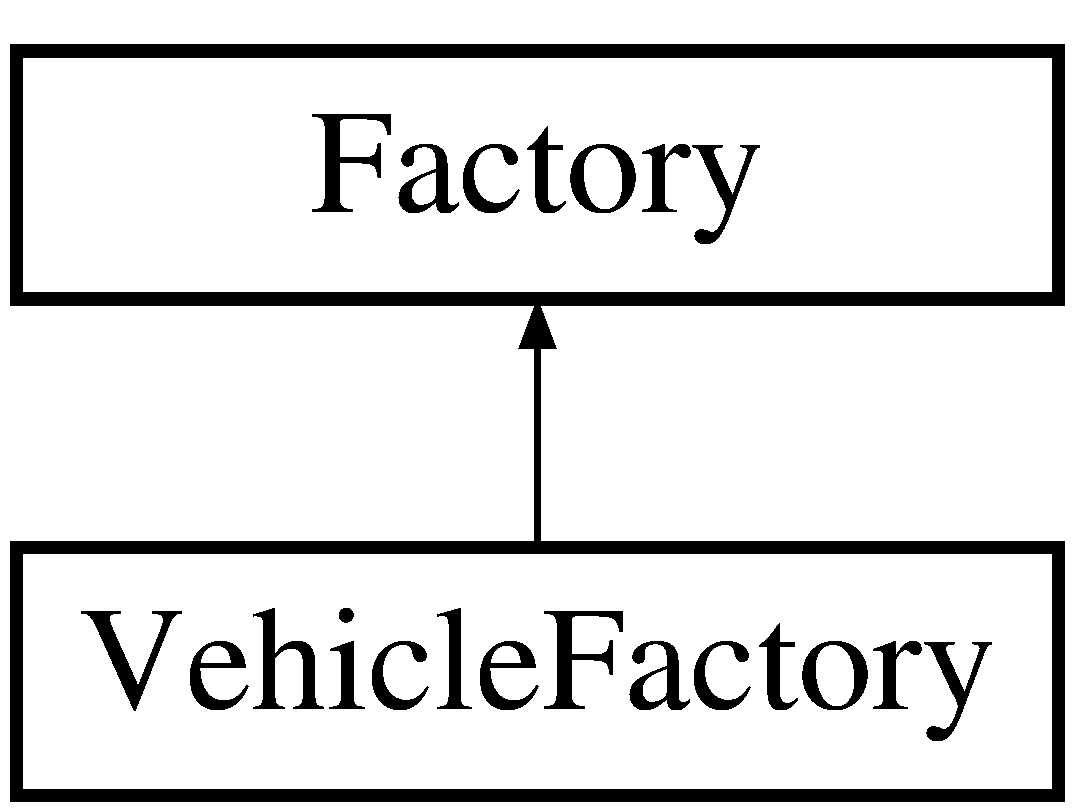
\includegraphics[height=2.000000cm]{classVehicleFactory}
\end{center}
\end{figure}
\doxysubsection*{Public Member Functions}
\begin{DoxyCompactItemize}
\item 
\mbox{\hyperlink{classVehicleFactory_a9bc9faf52aef1ad02193b3640b661f59}{Vehicle\+Factory}} (\mbox{\hyperlink{classType}{Type}} $\ast$type, \mbox{\hyperlink{classAddOn}{Add\+On}} $\ast$add\+On)
\begin{DoxyCompactList}\small\item\em Instantiates the vehicle factory. \end{DoxyCompactList}\item 
\mbox{\hyperlink{classEntity}{Entity}} $\ast$ \mbox{\hyperlink{classVehicleFactory_a3f34221921fd58cf83fd9bc8e3d8798f}{create\+Entity}} (\mbox{\hyperlink{classAlliance}{Alliance}} $\ast$alliance)
\begin{DoxyCompactList}\small\item\em Instantiates and returns a vehicle for the given alliance. \end{DoxyCompactList}\item 
\mbox{\hyperlink{classFactory}{Factory}} $\ast$ \mbox{\hyperlink{classVehicleFactory_a6d874e37b573b491a49e303209ac42cd}{clone}} ()
\begin{DoxyCompactList}\small\item\em Instantiates and returns a clone of the current vehicle factory. \end{DoxyCompactList}\end{DoxyCompactItemize}


\doxysubsection{Detailed Description}
\mbox{\hyperlink{classVehicleFactory}{Vehicle\+Factory}} class. 

Used to instantiate \mbox{\hyperlink{classVehicle}{Vehicle}} objects. 

Definition at line \mbox{\hyperlink{VehicleFactory_8h_source_l00010}{10}} of file \mbox{\hyperlink{VehicleFactory_8h_source}{Vehicle\+Factory.\+h}}.



\doxysubsection{Constructor \& Destructor Documentation}
\mbox{\Hypertarget{classVehicleFactory_a9bc9faf52aef1ad02193b3640b661f59}\label{classVehicleFactory_a9bc9faf52aef1ad02193b3640b661f59}} 
\index{VehicleFactory@{VehicleFactory}!VehicleFactory@{VehicleFactory}}
\index{VehicleFactory@{VehicleFactory}!VehicleFactory@{VehicleFactory}}
\doxysubsubsection{\texorpdfstring{VehicleFactory()}{VehicleFactory()}}
{\footnotesize\ttfamily Vehicle\+Factory\+::\+Vehicle\+Factory (\begin{DoxyParamCaption}\item[{\mbox{\hyperlink{classType}{Type}} $\ast$}]{type,  }\item[{\mbox{\hyperlink{classAddOn}{Add\+On}} $\ast$}]{add\+On }\end{DoxyParamCaption})}



Instantiates the vehicle factory. 


\begin{DoxyParams}{Parameters}
{\em type} & must be a Type$\ast$ \\
\hline
{\em add\+On} & must be a Add\+On$\ast$ \\
\hline
\end{DoxyParams}


Definition at line \mbox{\hyperlink{VehicleFactory_8cpp_source_l00004}{4}} of file \mbox{\hyperlink{VehicleFactory_8cpp_source}{Vehicle\+Factory.\+cpp}}.


\begin{DoxyCode}{0}
\DoxyCodeLine{00004 : \mbox{\hyperlink{classFactory}{Factory}}(type, addOn) \{\}}

\end{DoxyCode}


\doxysubsection{Member Function Documentation}
\mbox{\Hypertarget{classVehicleFactory_a6d874e37b573b491a49e303209ac42cd}\label{classVehicleFactory_a6d874e37b573b491a49e303209ac42cd}} 
\index{VehicleFactory@{VehicleFactory}!clone@{clone}}
\index{clone@{clone}!VehicleFactory@{VehicleFactory}}
\doxysubsubsection{\texorpdfstring{clone()}{clone()}}
{\footnotesize\ttfamily \mbox{\hyperlink{classFactory}{Factory}} $\ast$ Vehicle\+Factory\+::clone (\begin{DoxyParamCaption}{ }\end{DoxyParamCaption})\hspace{0.3cm}{\ttfamily [virtual]}}



Instantiates and returns a clone of the current vehicle factory. 

Postconditions\+:
\begin{DoxyItemize}
\item Returns the clone of the current vehicle factory
\end{DoxyItemize}

\begin{DoxyReturn}{Returns}
Factory$\ast$ The vehicle factory clone 
\end{DoxyReturn}


Implements \mbox{\hyperlink{classFactory}{Factory}}.



Definition at line \mbox{\hyperlink{VehicleFactory_8cpp_source_l00018}{18}} of file \mbox{\hyperlink{VehicleFactory_8cpp_source}{Vehicle\+Factory.\+cpp}}.


\begin{DoxyCode}{0}
\DoxyCodeLine{00018                                \{}
\DoxyCodeLine{00019     \textcolor{keywordflow}{return} \textcolor{keyword}{new} \mbox{\hyperlink{classVehicleFactory}{VehicleFactory}}(\mbox{\hyperlink{classFactory_ac91051006ace7ec5bb6ecf0fe6d02d58}{getType}}()-\/>\mbox{\hyperlink{classVehicleFactory_a6d874e37b573b491a49e303209ac42cd}{clone}}(), \mbox{\hyperlink{classFactory_a994153930f59cafb280e91d5b100b5aa}{getAddOn}}()-\/>\mbox{\hyperlink{classVehicleFactory_a6d874e37b573b491a49e303209ac42cd}{clone}}());}
\DoxyCodeLine{00020 \}}

\end{DoxyCode}
\mbox{\Hypertarget{classVehicleFactory_a3f34221921fd58cf83fd9bc8e3d8798f}\label{classVehicleFactory_a3f34221921fd58cf83fd9bc8e3d8798f}} 
\index{VehicleFactory@{VehicleFactory}!createEntity@{createEntity}}
\index{createEntity@{createEntity}!VehicleFactory@{VehicleFactory}}
\doxysubsubsection{\texorpdfstring{createEntity()}{createEntity()}}
{\footnotesize\ttfamily \mbox{\hyperlink{classEntity}{Entity}} $\ast$ Vehicle\+Factory\+::create\+Entity (\begin{DoxyParamCaption}\item[{\mbox{\hyperlink{classAlliance}{Alliance}} $\ast$}]{alliance }\end{DoxyParamCaption})\hspace{0.3cm}{\ttfamily [virtual]}}



Instantiates and returns a vehicle for the given alliance. 

Preconditions\+:
\begin{DoxyItemize}
\item alliance must be an Alliance$\ast$
\end{DoxyItemize}

Postconditions\+:
\begin{DoxyItemize}
\item Returns the instantiated vehicle object with specific state
\end{DoxyItemize}


\begin{DoxyParams}{Parameters}
{\em alliance} & must be a Alliance$\ast$ \\
\hline
\end{DoxyParams}
\begin{DoxyReturn}{Returns}
Vehicle$\ast$ The instatiated vehicle 
\end{DoxyReturn}


Implements \mbox{\hyperlink{classFactory}{Factory}}.



Definition at line \mbox{\hyperlink{VehicleFactory_8cpp_source_l00006}{6}} of file \mbox{\hyperlink{VehicleFactory_8cpp_source}{Vehicle\+Factory.\+cpp}}.


\begin{DoxyCode}{0}
\DoxyCodeLine{00006                                                        \{}
\DoxyCodeLine{00007     \mbox{\hyperlink{classVehicle}{Vehicle}}* v = \textcolor{keyword}{new} \mbox{\hyperlink{classVehicle}{Vehicle}}(\mbox{\hyperlink{classFactory_ac91051006ace7ec5bb6ecf0fe6d02d58}{getType}}()-\/>\mbox{\hyperlink{classVehicleFactory_a6d874e37b573b491a49e303209ac42cd}{clone}}());}
\DoxyCodeLine{00008     v-\/>\mbox{\hyperlink{classEntity_af804dcaa600e770cf0e2b4537f6fba23}{setAlliance}}(alliance);}
\DoxyCodeLine{00009     \textcolor{keywordflow}{if} (\mbox{\hyperlink{classFactory_a994153930f59cafb280e91d5b100b5aa}{getAddOn}}() != NULL) \{}
\DoxyCodeLine{00010         \mbox{\hyperlink{classAddOn}{AddOn}}* personnelAddOn = \mbox{\hyperlink{classFactory_a994153930f59cafb280e91d5b100b5aa}{getAddOn}}()-\/>clone();}
\DoxyCodeLine{00011         personnelAddOn-\/>\mbox{\hyperlink{classAddOn_ac9f4263e3558015fdad46adefceed197}{setEntity}}(v);}
\DoxyCodeLine{00012         \textcolor{keywordflow}{return} personnelAddOn;}
\DoxyCodeLine{00013     \} \textcolor{keywordflow}{else} \{}
\DoxyCodeLine{00014         \textcolor{keywordflow}{return} v;}
\DoxyCodeLine{00015     \}}
\DoxyCodeLine{00016 \}}

\end{DoxyCode}


The documentation for this class was generated from the following files\+:\begin{DoxyCompactItemize}
\item 
Vehicle\+Factory.\+h\item 
Vehicle\+Factory.\+cpp\end{DoxyCompactItemize}

\hypertarget{classWarEngine}{}\doxysection{War\+Engine Class Reference}
\label{classWarEngine}\index{WarEngine@{WarEngine}}
\doxysubsection*{Public Member Functions}
\begin{DoxyCompactItemize}
\item 
\mbox{\hyperlink{classWarEngineMemento}{War\+Engine\+Memento}} \mbox{\hyperlink{classWarEngine_a3ce98b4a76487348a712a4ffb54a71f2}{save\+State}} ()
\item 
void \mbox{\hyperlink{classWarEngine_a76994dd9d009fff3dd272a87710bfae5}{load\+State}} (\mbox{\hyperlink{classWarEngineState}{War\+Engine\+State}} save)
\end{DoxyCompactItemize}
\doxysubsection*{Protected Member Functions}
\begin{DoxyCompactItemize}
\item 
\mbox{\hyperlink{classWarEngine_a0c3e8e1ca61c1e85ffcbbaa26b9a749c}{War\+Engine}} (int \&war\+Engine)
\end{DoxyCompactItemize}


\doxysubsection{Detailed Description}


Definition at line \mbox{\hyperlink{WarEngine_8h_source_l00004}{4}} of file \mbox{\hyperlink{WarEngine_8h_source}{War\+Engine.\+h}}.



\doxysubsection{Constructor \& Destructor Documentation}
\mbox{\Hypertarget{classWarEngine_a3c95a6990a6eabd99f1ea0ade30f85f2}\label{classWarEngine_a3c95a6990a6eabd99f1ea0ade30f85f2}} 
\index{WarEngine@{WarEngine}!WarEngine@{WarEngine}}
\index{WarEngine@{WarEngine}!WarEngine@{WarEngine}}
\doxysubsubsection{\texorpdfstring{WarEngine()}{WarEngine()}\hspace{0.1cm}{\footnotesize\ttfamily [1/2]}}
{\footnotesize\ttfamily War\+Engine\+::\+War\+Engine (\begin{DoxyParamCaption}{ }\end{DoxyParamCaption})\hspace{0.3cm}{\ttfamily [protected]}}



Definition at line \mbox{\hyperlink{WarEngine_8cpp_source_l00003}{3}} of file \mbox{\hyperlink{WarEngine_8cpp_source}{War\+Engine.\+cpp}}.


\begin{DoxyCode}{0}
\DoxyCodeLine{00003                      \{}
\DoxyCodeLine{00004     \textcolor{comment}{// TODO -\/ implement WarEngine::WarEngine}}
\DoxyCodeLine{00005     \textcolor{keywordflow}{throw} \textcolor{stringliteral}{"{}Not yet implemented"{}};}
\DoxyCodeLine{00006 \}}

\end{DoxyCode}
\mbox{\Hypertarget{classWarEngine_a0c3e8e1ca61c1e85ffcbbaa26b9a749c}\label{classWarEngine_a0c3e8e1ca61c1e85ffcbbaa26b9a749c}} 
\index{WarEngine@{WarEngine}!WarEngine@{WarEngine}}
\index{WarEngine@{WarEngine}!WarEngine@{WarEngine}}
\doxysubsubsection{\texorpdfstring{WarEngine()}{WarEngine()}\hspace{0.1cm}{\footnotesize\ttfamily [2/2]}}
{\footnotesize\ttfamily War\+Engine\+::\+War\+Engine (\begin{DoxyParamCaption}\item[{int \&}]{war\+Engine }\end{DoxyParamCaption})\hspace{0.3cm}{\ttfamily [protected]}}



Definition at line \mbox{\hyperlink{WarEngine_8cpp_source_l00008}{8}} of file \mbox{\hyperlink{WarEngine_8cpp_source}{War\+Engine.\+cpp}}.


\begin{DoxyCode}{0}
\DoxyCodeLine{00008                                    \{}
\DoxyCodeLine{00009     \textcolor{comment}{// TODO -\/ implement WarEngine::WarEngine}}
\DoxyCodeLine{00010     \textcolor{keywordflow}{throw} \textcolor{stringliteral}{"{}Not yet implemented"{}};}
\DoxyCodeLine{00011 \}}

\end{DoxyCode}


\doxysubsection{Member Function Documentation}
\mbox{\Hypertarget{classWarEngine_a76994dd9d009fff3dd272a87710bfae5}\label{classWarEngine_a76994dd9d009fff3dd272a87710bfae5}} 
\index{WarEngine@{WarEngine}!loadState@{loadState}}
\index{loadState@{loadState}!WarEngine@{WarEngine}}
\doxysubsubsection{\texorpdfstring{loadState()}{loadState()}}
{\footnotesize\ttfamily void War\+Engine\+::load\+State (\begin{DoxyParamCaption}\item[{\mbox{\hyperlink{classWarEngineState}{War\+Engine\+State}}}]{save }\end{DoxyParamCaption})}



Definition at line \mbox{\hyperlink{WarEngine_8cpp_source_l00018}{18}} of file \mbox{\hyperlink{WarEngine_8cpp_source}{War\+Engine.\+cpp}}.


\begin{DoxyCode}{0}
\DoxyCodeLine{00018                                              \{}
\DoxyCodeLine{00019     \textcolor{comment}{// TODO -\/ implement WarEngine::loadState}}
\DoxyCodeLine{00020     \textcolor{keywordflow}{throw} \textcolor{stringliteral}{"{}Not yet implemented"{}};}
\DoxyCodeLine{00021 \}}

\end{DoxyCode}
\mbox{\Hypertarget{classWarEngine_a3ce98b4a76487348a712a4ffb54a71f2}\label{classWarEngine_a3ce98b4a76487348a712a4ffb54a71f2}} 
\index{WarEngine@{WarEngine}!saveState@{saveState}}
\index{saveState@{saveState}!WarEngine@{WarEngine}}
\doxysubsubsection{\texorpdfstring{saveState()}{saveState()}}
{\footnotesize\ttfamily \mbox{\hyperlink{classWarEngineMemento}{War\+Engine\+Memento}} War\+Engine\+::save\+State (\begin{DoxyParamCaption}{ }\end{DoxyParamCaption})}



Definition at line \mbox{\hyperlink{WarEngine_8cpp_source_l00013}{13}} of file \mbox{\hyperlink{WarEngine_8cpp_source}{War\+Engine.\+cpp}}.


\begin{DoxyCode}{0}
\DoxyCodeLine{00013                                       \{}
\DoxyCodeLine{00014     \textcolor{comment}{// TODO -\/ implement WarEngine::saveState}}
\DoxyCodeLine{00015     \textcolor{keywordflow}{throw} \textcolor{stringliteral}{"{}Not yet implemented"{}};}
\DoxyCodeLine{00016 \}}

\end{DoxyCode}


The documentation for this class was generated from the following files\+:\begin{DoxyCompactItemize}
\item 
War\+Engine.\+h\item 
War\+Engine.\+cpp\end{DoxyCompactItemize}

<<<<<<< HEAD
\hypertarget{classWarEngineMemento}{}\section{War\+Engine\+Memento Class Reference}
\label{classWarEngineMemento}\index{War\+Engine\+Memento@{War\+Engine\+Memento}}
=======
\hypertarget{classWarEngineMemento}{}\doxysection{War\+Engine\+Memento Class Reference}
\label{classWarEngineMemento}\index{WarEngineMemento@{WarEngineMemento}}
>>>>>>> 7be49738cebc0ced3357f2ce74f6fda2ea0b3d5e


{\ttfamily \#include $<$War\+Engine\+Memento.\+h$>$}

<<<<<<< HEAD
\subsection*{Friends}
\begin{DoxyCompactItemize}
\item 
\mbox{\Hypertarget{classWarEngineMemento_abc1564d646c3fdc348c5320f301d01ff}\label{classWarEngineMemento_abc1564d646c3fdc348c5320f301d01ff}} 
class {\bfseries War\+Engine}
=======
\doxysubsection*{Friends}
\begin{DoxyCompactItemize}
\item 
class \mbox{\hyperlink{classWarEngineMemento_abc1564d646c3fdc348c5320f301d01ff}{War\+Engine}}
>>>>>>> 7be49738cebc0ced3357f2ce74f6fda2ea0b3d5e
\end{DoxyCompactItemize}


\doxysubsection{Detailed Description}
Class that encapsulates and externalises \mbox{\hyperlink{classWarEngine}{War\+Engine}} State. 

<<<<<<< HEAD
Definition at line 15 of file War\+Engine\+Memento.\+h.



=======
Definition at line \mbox{\hyperlink{WarEngineMemento_8h_source_l00015}{15}} of file \mbox{\hyperlink{WarEngineMemento_8h_source}{War\+Engine\+Memento.\+h}}.



\doxysubsection{Friends And Related Function Documentation}
\mbox{\Hypertarget{classWarEngineMemento_abc1564d646c3fdc348c5320f301d01ff}\label{classWarEngineMemento_abc1564d646c3fdc348c5320f301d01ff}} 
\index{WarEngineMemento@{WarEngineMemento}!WarEngine@{WarEngine}}
\index{WarEngine@{WarEngine}!WarEngineMemento@{WarEngineMemento}}
\doxysubsubsection{\texorpdfstring{WarEngine}{WarEngine}}
{\footnotesize\ttfamily friend class \mbox{\hyperlink{classWarEngine}{War\+Engine}}\hspace{0.3cm}{\ttfamily [friend]}}



Definition at line \mbox{\hyperlink{WarEngineMemento_8h_source_l00017}{17}} of file \mbox{\hyperlink{WarEngineMemento_8h_source}{War\+Engine\+Memento.\+h}}.



>>>>>>> 7be49738cebc0ced3357f2ce74f6fda2ea0b3d5e
The documentation for this class was generated from the following files\+:\begin{DoxyCompactItemize}
\item 
War\+Engine\+Memento.\+h\item 
War\+Engine\+Memento.\+cpp\end{DoxyCompactItemize}

\hypertarget{classWarEngineState}{}\doxysection{War\+Engine\+State Class Reference}
\label{classWarEngineState}\index{WarEngineState@{WarEngineState}}


Class for storing current state of entire simulation.  




{\ttfamily \#include $<$War\+Engine\+State.\+h$>$}

\doxysubsection*{Public Member Functions}
\begin{DoxyCompactItemize}
\item 
\mbox{\hyperlink{classWarEngineState_a7cad5162c75ba597dfd8f4691e6049aa}{$\sim$\+War\+Engine\+State}} ()
\begin{DoxyCompactList}\small\item\em Destructor for class. \end{DoxyCompactList}\end{DoxyCompactItemize}
\doxysubsection*{Protected Member Functions}
\begin{DoxyCompactItemize}
\item 
\mbox{\hyperlink{classWarEngineState_a78b3ab46445c7abc7797531004cd6d67}{War\+Engine\+State}} ()
\begin{DoxyCompactList}\small\item\em Initializes an instance of the \mbox{\hyperlink{classWarEngineState}{War\+Engine\+State}} class. \end{DoxyCompactList}\item 
void \mbox{\hyperlink{classWarEngineState_af79cacdce276b52be3bedfe1a22c5f48}{set\+Area}} (\mbox{\hyperlink{classArea}{Area}} $\ast$area)
\begin{DoxyCompactList}\small\item\em Takes in a vector of \mbox{\hyperlink{classArea}{Area}} and sets it to the areas member of the \mbox{\hyperlink{classWarEngineState}{War\+Engine\+State}} instance. \end{DoxyCompactList}\item 
\mbox{\hyperlink{classArea}{Area}} $\ast$ \mbox{\hyperlink{classWarEngineState_a9c1fe3cc21780d0a8e1d82ce76fe7430}{get\+Area}} ()
\begin{DoxyCompactList}\small\item\em Returns the member variable area. \end{DoxyCompactList}\item 
void \mbox{\hyperlink{classWarEngineState_a262f8e5974144a644a24ca4edc949562}{set\+Alliances}} (vector$<$ \mbox{\hyperlink{classAlliance}{Alliance}} $\ast$ $>$ alliances)
\begin{DoxyCompactList}\small\item\em Sets the given vector of \mbox{\hyperlink{classAlliance}{Alliance}} object pointers to the alliances member variable. \end{DoxyCompactList}\item 
vector$<$ \mbox{\hyperlink{classAlliance}{Alliance}} $\ast$ $>$ \mbox{\hyperlink{classWarEngineState_aa88851d165886c80521e93c2d74338d5}{get\+Alliances}} ()
\begin{DoxyCompactList}\small\item\em Returns the alliances member variable. \end{DoxyCompactList}\item 
\mbox{\hyperlink{classWarEngineState}{War\+Engine\+State}} $\ast$ \mbox{\hyperlink{classWarEngineState_a89508b034ce4006ed830f671b525f745}{clone}} ()
\begin{DoxyCompactList}\small\item\em Returns a clone of the current \mbox{\hyperlink{classWarEngineMemento}{War\+Engine\+Memento}} object. \end{DoxyCompactList}\end{DoxyCompactItemize}
\doxysubsection*{Friends}
\begin{DoxyCompactItemize}
\item 
class \mbox{\hyperlink{classWarEngineState_abc1564d646c3fdc348c5320f301d01ff}{War\+Engine}}
\end{DoxyCompactItemize}


\doxysubsection{Detailed Description}
Class for storing current state of entire simulation. 

Class contains member variables areas which stores a vector of all war theatres and keypoints as well as a vector of all alliances in current simulation. 

Definition at line \mbox{\hyperlink{WarEngineState_8h_source_l00017}{17}} of file \mbox{\hyperlink{WarEngineState_8h_source}{War\+Engine\+State.\+h}}.



\doxysubsection{Constructor \& Destructor Documentation}
\mbox{\Hypertarget{classWarEngineState_a78b3ab46445c7abc7797531004cd6d67}\label{classWarEngineState_a78b3ab46445c7abc7797531004cd6d67}} 
\index{WarEngineState@{WarEngineState}!WarEngineState@{WarEngineState}}
\index{WarEngineState@{WarEngineState}!WarEngineState@{WarEngineState}}
\doxysubsubsection{\texorpdfstring{WarEngineState()}{WarEngineState()}}
{\footnotesize\ttfamily War\+Engine\+State\+::\+War\+Engine\+State (\begin{DoxyParamCaption}{ }\end{DoxyParamCaption})\hspace{0.3cm}{\ttfamily [protected]}}



Initializes an instance of the \mbox{\hyperlink{classWarEngineState}{War\+Engine\+State}} class. 



Definition at line \mbox{\hyperlink{WarEngineState_8cpp_source_l00003}{3}} of file \mbox{\hyperlink{WarEngineState_8cpp_source}{War\+Engine\+State.\+cpp}}.


\begin{DoxyCode}{0}
\DoxyCodeLine{00003                                \{}
\DoxyCodeLine{00004     area = \textcolor{keyword}{nullptr};}
\DoxyCodeLine{00005 \}}

\end{DoxyCode}
\mbox{\Hypertarget{classWarEngineState_a7cad5162c75ba597dfd8f4691e6049aa}\label{classWarEngineState_a7cad5162c75ba597dfd8f4691e6049aa}} 
\index{WarEngineState@{WarEngineState}!````~WarEngineState@{$\sim$WarEngineState}}
\index{````~WarEngineState@{$\sim$WarEngineState}!WarEngineState@{WarEngineState}}
\doxysubsubsection{\texorpdfstring{$\sim$WarEngineState()}{~WarEngineState()}}
{\footnotesize\ttfamily War\+Engine\+State\+::$\sim$\+War\+Engine\+State (\begin{DoxyParamCaption}{ }\end{DoxyParamCaption})}



Destructor for class. 



Definition at line \mbox{\hyperlink{WarEngineState_8cpp_source_l00048}{48}} of file \mbox{\hyperlink{WarEngineState_8cpp_source}{War\+Engine\+State.\+cpp}}.


\begin{DoxyCode}{0}
\DoxyCodeLine{00048                                \{}
\DoxyCodeLine{00049 }
\DoxyCodeLine{00050     \textcolor{keywordflow}{for}(\mbox{\hyperlink{classAlliance}{Alliance}}* alliance : this-\/>alliances)\{}
\DoxyCodeLine{00051         \textcolor{keyword}{delete} alliance;}
\DoxyCodeLine{00052     \}}
\DoxyCodeLine{00053 }
\DoxyCodeLine{00054     \textcolor{keyword}{delete} this-\/>area;}
\DoxyCodeLine{00055 \}}

\end{DoxyCode}


\doxysubsection{Member Function Documentation}
\mbox{\Hypertarget{classWarEngineState_a89508b034ce4006ed830f671b525f745}\label{classWarEngineState_a89508b034ce4006ed830f671b525f745}} 
\index{WarEngineState@{WarEngineState}!clone@{clone}}
\index{clone@{clone}!WarEngineState@{WarEngineState}}
\doxysubsubsection{\texorpdfstring{clone()}{clone()}}
{\footnotesize\ttfamily \mbox{\hyperlink{classWarEngineState}{War\+Engine\+State}} $\ast$ War\+Engine\+State\+::clone (\begin{DoxyParamCaption}{ }\end{DoxyParamCaption})\hspace{0.3cm}{\ttfamily [protected]}}



Returns a clone of the current \mbox{\hyperlink{classWarEngineMemento}{War\+Engine\+Memento}} object. 

\begin{DoxyReturn}{Returns}
War\+Engine\+State$\ast$ 
\end{DoxyReturn}


Definition at line \mbox{\hyperlink{WarEngineState_8cpp_source_l00031}{31}} of file \mbox{\hyperlink{WarEngineState_8cpp_source}{War\+Engine\+State.\+cpp}}.


\begin{DoxyCode}{0}
\DoxyCodeLine{00031                                      \{}
\DoxyCodeLine{00032 }
\DoxyCodeLine{00033     \mbox{\hyperlink{classWarEngineState}{WarEngineState}}* clonedState = \textcolor{keyword}{new} \mbox{\hyperlink{classWarEngineState_a78b3ab46445c7abc7797531004cd6d67}{WarEngineState}}();}
\DoxyCodeLine{00034 }
\DoxyCodeLine{00035     clonedState-\/>\mbox{\hyperlink{classWarEngineState_af79cacdce276b52be3bedfe1a22c5f48}{setArea}}( this-\/>area-\/>\mbox{\hyperlink{classArea_a8f95bd4832e9534e645403975435b11d}{clone}}() );}
\DoxyCodeLine{00036 }
\DoxyCodeLine{00037     \textcolor{keywordflow}{for}(\mbox{\hyperlink{classAlliance}{Alliance}}* alliance : this-\/>alliances)\{}
\DoxyCodeLine{00038         }
\DoxyCodeLine{00039         \mbox{\hyperlink{classAlliance}{Alliance}}* clonedAlliance = alliance-\/>\mbox{\hyperlink{classAlliance_adc67a41223565105889493f9cfd350d0}{clone}}();}
\DoxyCodeLine{00040 }
\DoxyCodeLine{00041         clonedState-\/>alliances.push\_back(alliance);}
\DoxyCodeLine{00042 }
\DoxyCodeLine{00043     \}}
\DoxyCodeLine{00044 }
\DoxyCodeLine{00045         \textcolor{keywordflow}{return} clonedState;}
\DoxyCodeLine{00046     \}}

\end{DoxyCode}
\mbox{\Hypertarget{classWarEngineState_aa88851d165886c80521e93c2d74338d5}\label{classWarEngineState_aa88851d165886c80521e93c2d74338d5}} 
\index{WarEngineState@{WarEngineState}!getAlliances@{getAlliances}}
\index{getAlliances@{getAlliances}!WarEngineState@{WarEngineState}}
\doxysubsubsection{\texorpdfstring{getAlliances()}{getAlliances()}}
{\footnotesize\ttfamily vector$<$ \mbox{\hyperlink{classAlliance}{Alliance}} $\ast$ $>$ War\+Engine\+State\+::get\+Alliances (\begin{DoxyParamCaption}{ }\end{DoxyParamCaption})\hspace{0.3cm}{\ttfamily [protected]}}



Returns the alliances member variable. 

\begin{DoxyReturn}{Returns}
vector \texorpdfstring{$<$}{<}Alliance$\ast$\texorpdfstring{$>$}{>}
\end{DoxyReturn}

\begin{DoxyExceptions}{Exceptions}
{\em out\+\_\+of\+\_\+range} & save archive is empty \\
\hline
\end{DoxyExceptions}


Definition at line \mbox{\hyperlink{WarEngineState_8cpp_source_l00023}{23}} of file \mbox{\hyperlink{WarEngineState_8cpp_source}{War\+Engine\+State.\+cpp}}.


\begin{DoxyCode}{0}
\DoxyCodeLine{00023                                                \{}
\DoxyCodeLine{00024 }
\DoxyCodeLine{00025     \textcolor{keywordflow}{if}(alliances.size() == 0)}
\DoxyCodeLine{00026         std::\_\_throw\_out\_of\_range(\textcolor{stringliteral}{"{}No Alliances stored."{}});}
\DoxyCodeLine{00027 }
\DoxyCodeLine{00028     \textcolor{keywordflow}{return} alliances;}
\DoxyCodeLine{00029 \}}

\end{DoxyCode}
\mbox{\Hypertarget{classWarEngineState_a9c1fe3cc21780d0a8e1d82ce76fe7430}\label{classWarEngineState_a9c1fe3cc21780d0a8e1d82ce76fe7430}} 
\index{WarEngineState@{WarEngineState}!getArea@{getArea}}
\index{getArea@{getArea}!WarEngineState@{WarEngineState}}
\doxysubsubsection{\texorpdfstring{getArea()}{getArea()}}
{\footnotesize\ttfamily \mbox{\hyperlink{classArea}{Area}} $\ast$ War\+Engine\+State\+::get\+Area (\begin{DoxyParamCaption}{ }\end{DoxyParamCaption})\hspace{0.3cm}{\ttfamily [protected]}}



Returns the member variable area. 

Postconditions\+:
\begin{DoxyItemize}
\item Retruns the area stored in the state
\end{DoxyItemize}

\begin{DoxyReturn}{Returns}
Area$\ast$ 
\end{DoxyReturn}


Definition at line \mbox{\hyperlink{WarEngineState_8cpp_source_l00011}{11}} of file \mbox{\hyperlink{WarEngineState_8cpp_source}{War\+Engine\+State.\+cpp}}.


\begin{DoxyCode}{0}
\DoxyCodeLine{00011                               \{}
\DoxyCodeLine{00012 }
\DoxyCodeLine{00013     \textcolor{keywordflow}{if}(area == \textcolor{keyword}{nullptr})}
\DoxyCodeLine{00014         \textcolor{keywordflow}{throw} \textcolor{stringliteral}{"{}No Areas Stored."{}};}
\DoxyCodeLine{00015 }
\DoxyCodeLine{00016     \textcolor{keywordflow}{return} this-\/>area;}
\DoxyCodeLine{00017 \}}

\end{DoxyCode}
\mbox{\Hypertarget{classWarEngineState_a262f8e5974144a644a24ca4edc949562}\label{classWarEngineState_a262f8e5974144a644a24ca4edc949562}} 
\index{WarEngineState@{WarEngineState}!setAlliances@{setAlliances}}
\index{setAlliances@{setAlliances}!WarEngineState@{WarEngineState}}
\doxysubsubsection{\texorpdfstring{setAlliances()}{setAlliances()}}
{\footnotesize\ttfamily void War\+Engine\+State\+::set\+Alliances (\begin{DoxyParamCaption}\item[{vector$<$ \mbox{\hyperlink{classAlliance}{Alliance}} $\ast$ $>$}]{alliances }\end{DoxyParamCaption})\hspace{0.3cm}{\ttfamily [protected]}}



Sets the given vector of \mbox{\hyperlink{classAlliance}{Alliance}} object pointers to the alliances member variable. 


\begin{DoxyParams}{Parameters}
{\em vector$<$\+Alliance$\ast$$>$} & alliances\\
\hline
\end{DoxyParams}
Preconditions\+:
\begin{DoxyItemize}
\item alliances must be a vector of Alliance$\ast$
\end{DoxyItemize}

Postconditions\+:
\begin{DoxyItemize}
\item Sets the instance\textquotesingle{}s alliances member variable to the passed in parameter.
\end{DoxyItemize}

\begin{DoxyReturn}{Returns}
void 
\end{DoxyReturn}


Definition at line \mbox{\hyperlink{WarEngineState_8cpp_source_l00019}{19}} of file \mbox{\hyperlink{WarEngineState_8cpp_source}{War\+Engine\+State.\+cpp}}.


\begin{DoxyCode}{0}
\DoxyCodeLine{00019                                                              \{}
\DoxyCodeLine{00020     this-\/>alliances = alliances;}
\DoxyCodeLine{00021 \}}

\end{DoxyCode}
\mbox{\Hypertarget{classWarEngineState_af79cacdce276b52be3bedfe1a22c5f48}\label{classWarEngineState_af79cacdce276b52be3bedfe1a22c5f48}} 
\index{WarEngineState@{WarEngineState}!setArea@{setArea}}
\index{setArea@{setArea}!WarEngineState@{WarEngineState}}
\doxysubsubsection{\texorpdfstring{setArea()}{setArea()}}
{\footnotesize\ttfamily void War\+Engine\+State\+::set\+Area (\begin{DoxyParamCaption}\item[{\mbox{\hyperlink{classArea}{Area}} $\ast$}]{area }\end{DoxyParamCaption})\hspace{0.3cm}{\ttfamily [protected]}}



Takes in a vector of \mbox{\hyperlink{classArea}{Area}} and sets it to the areas member of the \mbox{\hyperlink{classWarEngineState}{War\+Engine\+State}} instance. 

Preconditions\+:
\begin{DoxyItemize}
\item area must be of type Area$\ast$
\end{DoxyItemize}

Postconditions\+:
\begin{DoxyItemize}
\item Sets the \mbox{\hyperlink{classWarEngineState}{War\+Engine\+State}} area member variable to the passed in parameter.
\end{DoxyItemize}


\begin{DoxyParams}{Parameters}
{\em area} & must be an Area$\ast$ \\
\hline
\end{DoxyParams}
\begin{DoxyReturn}{Returns}
void 
\end{DoxyReturn}


Definition at line \mbox{\hyperlink{WarEngineState_8cpp_source_l00007}{7}} of file \mbox{\hyperlink{WarEngineState_8cpp_source}{War\+Engine\+State.\+cpp}}.


\begin{DoxyCode}{0}
\DoxyCodeLine{00007                                        \{}
\DoxyCodeLine{00008     this-\/>area = area;}
\DoxyCodeLine{00009 \}}

\end{DoxyCode}


\doxysubsection{Friends And Related Function Documentation}
\mbox{\Hypertarget{classWarEngineState_abc1564d646c3fdc348c5320f301d01ff}\label{classWarEngineState_abc1564d646c3fdc348c5320f301d01ff}} 
\index{WarEngineState@{WarEngineState}!WarEngine@{WarEngine}}
\index{WarEngine@{WarEngine}!WarEngineState@{WarEngineState}}
\doxysubsubsection{\texorpdfstring{WarEngine}{WarEngine}}
{\footnotesize\ttfamily friend class \mbox{\hyperlink{classWarEngine}{War\+Engine}}\hspace{0.3cm}{\ttfamily [friend]}}



Definition at line \mbox{\hyperlink{WarEngineState_8h_source_l00018}{18}} of file \mbox{\hyperlink{WarEngineState_8h_source}{War\+Engine\+State.\+h}}.



The documentation for this class was generated from the following files\+:\begin{DoxyCompactItemize}
\item 
War\+Engine\+State.\+h\item 
War\+Engine\+State.\+cpp\end{DoxyCompactItemize}

\hypertarget{classWarTheatre}{}\doxysection{War\+Theatre Class Reference}
\label{classWarTheatre}\index{WarTheatre@{WarTheatre}}
Inheritance diagram for War\+Theatre\+:\begin{figure}[H]
\begin{center}
\leavevmode
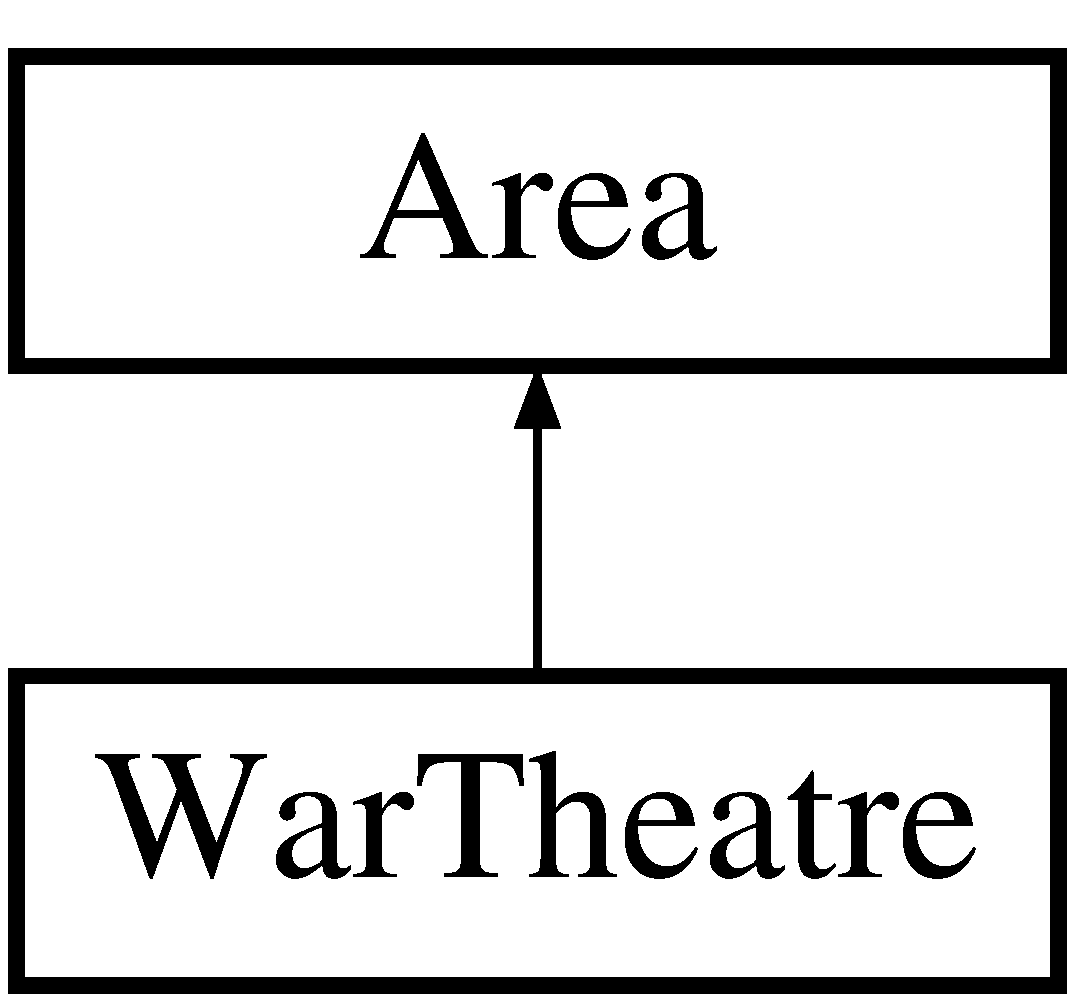
\includegraphics[height=2.000000cm]{classWarTheatre}
\end{center}
\end{figure}
\doxysubsection*{Public Member Functions}
\begin{DoxyCompactItemize}
\item 
\mbox{\hyperlink{classWarTheatre_aeac00db856afa4a7223d265093c7eca2}{War\+Theatre}} ()
\begin{DoxyCompactList}\small\item\em Instantiates the war theatre. \end{DoxyCompactList}\item 
void \mbox{\hyperlink{classWarTheatre_a4be07a7321747894bd035ec130a06c56}{$\sim$\+War\+Theatre}} ()
\begin{DoxyCompactList}\small\item\em Destroys the war theatre object. \end{DoxyCompactList}\item 
bool \mbox{\hyperlink{classWarTheatre_a01845ca2cc01367101b2884f2902bf88}{is\+Key\+Point}} ()
\begin{DoxyCompactList}\small\item\em Returns area type. \end{DoxyCompactList}\item 
void \mbox{\hyperlink{classWarTheatre_a9c1a612347b0da87a0421e37f6b7b12b}{attack}} (\mbox{\hyperlink{classAlliance}{Alliance}} $\ast$alliance)
\begin{DoxyCompactList}\small\item\em Attack with troops from the alliance passed in. \end{DoxyCompactList}\item 
void \mbox{\hyperlink{classWarTheatre_ab26cd475022390aefc1e4c6475e194ac}{move\+Entities}} (\mbox{\hyperlink{classArea}{Area}} $\ast$area, \mbox{\hyperlink{classAlliance}{Alliance}} $\ast$alliance)
\begin{DoxyCompactList}\small\item\em Moves a specific alliances troops from one area to another. \end{DoxyCompactList}\item 
void \mbox{\hyperlink{classWarTheatre_adc871336a6bf1263216b0f87da04cc57}{add\+Area}} (\mbox{\hyperlink{classArea}{Area}} $\ast$area)
\begin{DoxyCompactList}\small\item\em Adds an area to the war theatre object. \end{DoxyCompactList}\item 
\mbox{\hyperlink{classArea}{Area}} $\ast$ \mbox{\hyperlink{classWarTheatre_a501f851edf6f5ad00770414e50505175}{clone}} ()
\end{DoxyCompactItemize}


\doxysubsection{Detailed Description}


Definition at line \mbox{\hyperlink{WarTheatre_8h_source_l00004}{4}} of file \mbox{\hyperlink{WarTheatre_8h_source}{War\+Theatre.\+h}}.



\doxysubsection{Constructor \& Destructor Documentation}
\mbox{\Hypertarget{classWarTheatre_aeac00db856afa4a7223d265093c7eca2}\label{classWarTheatre_aeac00db856afa4a7223d265093c7eca2}} 
\index{WarTheatre@{WarTheatre}!WarTheatre@{WarTheatre}}
\index{WarTheatre@{WarTheatre}!WarTheatre@{WarTheatre}}
\doxysubsubsection{\texorpdfstring{WarTheatre()}{WarTheatre()}}
{\footnotesize\ttfamily War\+Theatre\+::\+War\+Theatre (\begin{DoxyParamCaption}{ }\end{DoxyParamCaption})}



Instantiates the war theatre. 



Definition at line \mbox{\hyperlink{WarTheatre_8cpp_source_l00003}{3}} of file \mbox{\hyperlink{WarTheatre_8cpp_source}{War\+Theatre.\+cpp}}.


\begin{DoxyCode}{0}
\DoxyCodeLine{00003                        \{}
\DoxyCodeLine{00004     \textcolor{comment}{// TODO -\/ implement WarTheatre::WarTheatre}}
\DoxyCodeLine{00005     \textcolor{keywordflow}{throw} \textcolor{stringliteral}{"{}Not yet implemented"{}};}
\DoxyCodeLine{00006 \}}

\end{DoxyCode}
\mbox{\Hypertarget{classWarTheatre_a4be07a7321747894bd035ec130a06c56}\label{classWarTheatre_a4be07a7321747894bd035ec130a06c56}} 
\index{WarTheatre@{WarTheatre}!````~WarTheatre@{$\sim$WarTheatre}}
\index{````~WarTheatre@{$\sim$WarTheatre}!WarTheatre@{WarTheatre}}
\doxysubsubsection{\texorpdfstring{$\sim$WarTheatre()}{~WarTheatre()}}
{\footnotesize\ttfamily void War\+Theatre\+::$\sim$\+War\+Theatre (\begin{DoxyParamCaption}{ }\end{DoxyParamCaption})}



Destroys the war theatre object. 

Postconditions\+:
\begin{DoxyItemize}
\item All dynamic memory should be deallocated from the war theatre object 
\end{DoxyItemize}

\doxysubsection{Member Function Documentation}
\mbox{\Hypertarget{classWarTheatre_adc871336a6bf1263216b0f87da04cc57}\label{classWarTheatre_adc871336a6bf1263216b0f87da04cc57}} 
\index{WarTheatre@{WarTheatre}!addArea@{addArea}}
\index{addArea@{addArea}!WarTheatre@{WarTheatre}}
\doxysubsubsection{\texorpdfstring{addArea()}{addArea()}}
{\footnotesize\ttfamily void War\+Theatre\+::add\+Area (\begin{DoxyParamCaption}\item[{\mbox{\hyperlink{classArea}{Area}} $\ast$}]{area }\end{DoxyParamCaption})}



Adds an area to the war theatre object. 

Preconditions\+:
\begin{DoxyItemize}
\item area must be an Area$\ast$
\end{DoxyItemize}

Postconditions\+:
\begin{DoxyItemize}
\item Add area to war theatre object
\end{DoxyItemize}


\begin{DoxyParams}{Parameters}
{\em area} & must be an Area$\ast$ \\
\hline
\end{DoxyParams}
\begin{DoxyReturn}{Returns}
void 
\end{DoxyReturn}


Definition at line \mbox{\hyperlink{WarTheatre_8cpp_source_l00023}{23}} of file \mbox{\hyperlink{WarTheatre_8cpp_source}{War\+Theatre.\+cpp}}.


\begin{DoxyCode}{0}
\DoxyCodeLine{00023                                    \{}
\DoxyCodeLine{00024     \textcolor{comment}{// TODO -\/ implement WarTheatre::addArea}}
\DoxyCodeLine{00025     \textcolor{keywordflow}{throw} \textcolor{stringliteral}{"{}Not yet implemented"{}};}
\DoxyCodeLine{00026 \}}

\end{DoxyCode}
\mbox{\Hypertarget{classWarTheatre_a9c1a612347b0da87a0421e37f6b7b12b}\label{classWarTheatre_a9c1a612347b0da87a0421e37f6b7b12b}} 
\index{WarTheatre@{WarTheatre}!attack@{attack}}
\index{attack@{attack}!WarTheatre@{WarTheatre}}
\doxysubsubsection{\texorpdfstring{attack()}{attack()}}
{\footnotesize\ttfamily void War\+Theatre\+::attack (\begin{DoxyParamCaption}\item[{\mbox{\hyperlink{classAlliance}{Alliance}} $\ast$}]{alliance }\end{DoxyParamCaption})\hspace{0.3cm}{\ttfamily [virtual]}}



Attack with troops from the alliance passed in. 

Preconditions\+:
\begin{DoxyItemize}
\item alliance must be an Alliance$\ast$
\end{DoxyItemize}

Postconditions\+:
\begin{DoxyItemize}
\item Call attacks function of areas
\end{DoxyItemize}


\begin{DoxyParams}{Parameters}
{\em alliance} & must be an Alliance$\ast$ \\
\hline
\end{DoxyParams}
\begin{DoxyReturn}{Returns}
void 
\end{DoxyReturn}


Implements \mbox{\hyperlink{classArea}{Area}}.



Definition at line \mbox{\hyperlink{WarTheatre_8cpp_source_l00013}{13}} of file \mbox{\hyperlink{WarTheatre_8cpp_source}{War\+Theatre.\+cpp}}.


\begin{DoxyCode}{0}
\DoxyCodeLine{00013                                           \{}
\DoxyCodeLine{00014     \textcolor{comment}{// TODO -\/ implement WarTheatre::attack}}
\DoxyCodeLine{00015     \textcolor{keywordflow}{throw} \textcolor{stringliteral}{"{}Not yet implemented"{}};}
\DoxyCodeLine{00016 \}}

\end{DoxyCode}
\mbox{\Hypertarget{classWarTheatre_a501f851edf6f5ad00770414e50505175}\label{classWarTheatre_a501f851edf6f5ad00770414e50505175}} 
\index{WarTheatre@{WarTheatre}!clone@{clone}}
\index{clone@{clone}!WarTheatre@{WarTheatre}}
\doxysubsubsection{\texorpdfstring{clone()}{clone()}}
{\footnotesize\ttfamily \mbox{\hyperlink{classArea}{Area}} $\ast$ War\+Theatre\+::clone (\begin{DoxyParamCaption}{ }\end{DoxyParamCaption})\hspace{0.3cm}{\ttfamily [virtual]}}



Implements \mbox{\hyperlink{classArea}{Area}}.



Definition at line \mbox{\hyperlink{WarTheatre_8cpp_source_l00028}{28}} of file \mbox{\hyperlink{WarTheatre_8cpp_source}{War\+Theatre.\+cpp}}.


\begin{DoxyCode}{0}
\DoxyCodeLine{00028                         \{}
\DoxyCodeLine{00029     \textcolor{comment}{// TODO -\/ implement WarTheatre::clone}}
\DoxyCodeLine{00030     \textcolor{keywordflow}{throw} \textcolor{stringliteral}{"{}Not yet implemented"{}};}
\DoxyCodeLine{00031 \}}

\end{DoxyCode}
\mbox{\Hypertarget{classWarTheatre_a01845ca2cc01367101b2884f2902bf88}\label{classWarTheatre_a01845ca2cc01367101b2884f2902bf88}} 
\index{WarTheatre@{WarTheatre}!isKeyPoint@{isKeyPoint}}
\index{isKeyPoint@{isKeyPoint}!WarTheatre@{WarTheatre}}
\doxysubsubsection{\texorpdfstring{isKeyPoint()}{isKeyPoint()}}
{\footnotesize\ttfamily bool War\+Theatre\+::is\+Key\+Point (\begin{DoxyParamCaption}{ }\end{DoxyParamCaption})\hspace{0.3cm}{\ttfamily [virtual]}}



Returns area type. 

Postconditions\+:
\begin{DoxyItemize}
\item Returns false
\end{DoxyItemize}

\begin{DoxyReturn}{Returns}
bool The area type 
\end{DoxyReturn}


Implements \mbox{\hyperlink{classArea}{Area}}.



Definition at line \mbox{\hyperlink{WarTheatre_8cpp_source_l00008}{8}} of file \mbox{\hyperlink{WarTheatre_8cpp_source}{War\+Theatre.\+cpp}}.


\begin{DoxyCode}{0}
\DoxyCodeLine{00008                             \{}
\DoxyCodeLine{00009     \textcolor{comment}{// TODO -\/ implement WarTheatre::isKeyPoint}}
\DoxyCodeLine{00010     \textcolor{keywordflow}{throw} \textcolor{stringliteral}{"{}Not yet implemented"{}};}
\DoxyCodeLine{00011 \}}

\end{DoxyCode}
\mbox{\Hypertarget{classWarTheatre_ab26cd475022390aefc1e4c6475e194ac}\label{classWarTheatre_ab26cd475022390aefc1e4c6475e194ac}} 
\index{WarTheatre@{WarTheatre}!moveEntities@{moveEntities}}
\index{moveEntities@{moveEntities}!WarTheatre@{WarTheatre}}
\doxysubsubsection{\texorpdfstring{moveEntities()}{moveEntities()}}
{\footnotesize\ttfamily void War\+Theatre\+::move\+Entities (\begin{DoxyParamCaption}\item[{\mbox{\hyperlink{classArea}{Area}} $\ast$}]{area,  }\item[{\mbox{\hyperlink{classAlliance}{Alliance}} $\ast$}]{alliance }\end{DoxyParamCaption})\hspace{0.3cm}{\ttfamily [virtual]}}



Moves a specific alliances troops from one area to another. 

Preconditions\+:
\begin{DoxyItemize}
\item area must be an Area$\ast$
\end{DoxyItemize}

alliance must be an Alliance$\ast$

Postconditions\+:
\begin{DoxyItemize}
\item Call move troops function on correct area
\end{DoxyItemize}


\begin{DoxyParams}{Parameters}
{\em area} & musy be an Area$\ast$ \\
\hline
{\em alliance} & must be an Alliance$\ast$ \\
\hline
\end{DoxyParams}
\begin{DoxyReturn}{Returns}
void 
\end{DoxyReturn}


Implements \mbox{\hyperlink{classArea}{Area}}.



Definition at line \mbox{\hyperlink{WarTheatre_8cpp_source_l00018}{18}} of file \mbox{\hyperlink{WarTheatre_8cpp_source}{War\+Theatre.\+cpp}}.


\begin{DoxyCode}{0}
\DoxyCodeLine{00018                                                             \{}
\DoxyCodeLine{00019     \textcolor{comment}{// TODO -\/ implement WarTheatre::moveEntities}}
\DoxyCodeLine{00020     \textcolor{keywordflow}{throw} \textcolor{stringliteral}{"{}Not yet implemented"{}};}
\DoxyCodeLine{00021 \}}

\end{DoxyCode}


The documentation for this class was generated from the following files\+:\begin{DoxyCompactItemize}
\item 
War\+Theatre.\+h\item 
War\+Theatre.\+cpp\end{DoxyCompactItemize}

\hypertarget{classWeather}{}\section{Weather Class Reference}
\label{classWeather}\index{Weather@{Weather}}
Inheritance diagram for Weather\+:\begin{figure}[H]
\begin{center}
\leavevmode
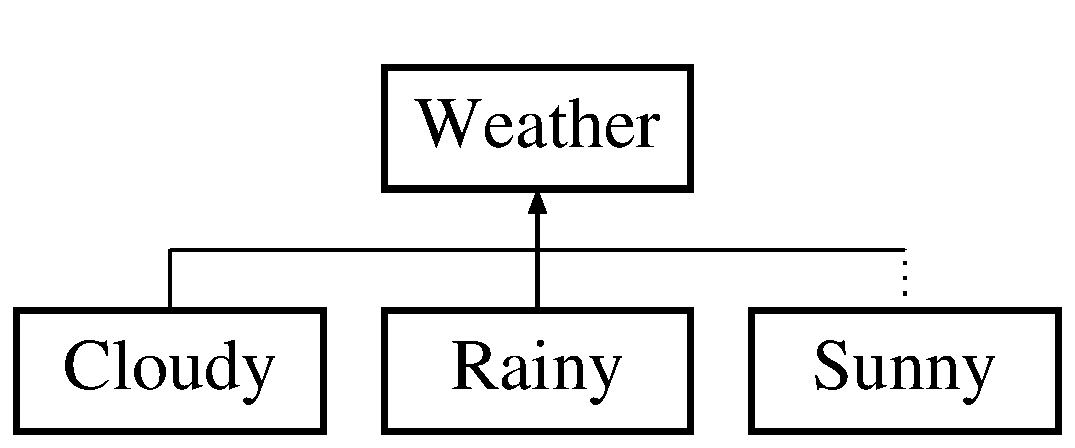
\includegraphics[height=2.000000cm]{classWeather}
\end{center}
\end{figure}
\subsection*{Public Member Functions}
\begin{DoxyCompactItemize}
\item 
\mbox{\Hypertarget{classWeather_af697ebc3ce0db3c7c6bc9b45854114e7}\label{classWeather_af697ebc3ce0db3c7c6bc9b45854114e7}} 
virtual void {\bfseries handle\+Change} (\hyperlink{classKeyPoint}{Key\+Point} $\ast$k)=0
\item 
\mbox{\Hypertarget{classWeather_ad7209dc331c4acdcdf7f17a94212eccb}\label{classWeather_ad7209dc331c4acdcdf7f17a94212eccb}} 
virtual string {\bfseries get\+Weather} ()=0
\end{DoxyCompactItemize}


\subsection{Detailed Description}


Definition at line 4 of file Weather.\+h.



The documentation for this class was generated from the following files\+:\begin{DoxyCompactItemize}
\item 
Weather.\+h\item 
Weather.\+cpp\end{DoxyCompactItemize}

%--- End generated contents ---

% Index
\backmatter
\newpage
\phantomsection
\clearemptydoublepage
\addcontentsline{toc}{chapter}{Index}
\printindex

\end{document}
